% Options for packages loaded elsewhere
\PassOptionsToPackage{unicode}{hyperref}
\PassOptionsToPackage{hyphens}{url}
\PassOptionsToPackage{dvipsnames,svgnames,x11names}{xcolor}
%
\documentclass[
]{article}
\title{Trading social status for genetics in marriage markets: evidence from UK Biobank}
\author{Abdel Abdellaoui\thanks{Department of Psychiatry, Amsterdam UMC, University 
of Amsterdam, Amsterdam, The Netherlands. Email: a.abdellaoui@amsterdamumc.nl},
Oana Borcan\thanks{School of Economics, University of East Anglia, Norwich, 
UK. Email: O.Borcan@uea.ac.uk} \&
David Hugh-Jones\thanks{Corresponding author. School of Economics, 
University of East Anglia, Norwich, UK. Email: D.Hugh-Jones@uea.ac.uk}}
\date{2021-11-17}

\usepackage{amsmath,amssymb}
\usepackage{lmodern}
\usepackage{iftex}
\ifPDFTeX
  \usepackage[T1]{fontenc}
  \usepackage[utf8]{inputenc}
  \usepackage{textcomp} % provide euro and other symbols
\else % if luatex or xetex
  \usepackage{unicode-math}
  \defaultfontfeatures{Scale=MatchLowercase}
  \defaultfontfeatures[\rmfamily]{Ligatures=TeX,Scale=1}
  \setmainfont[]{Times}
\fi
% Use upquote if available, for straight quotes in verbatim environments
\IfFileExists{upquote.sty}{\usepackage{upquote}}{}
\IfFileExists{microtype.sty}{% use microtype if available
  \usepackage[]{microtype}
  \UseMicrotypeSet[protrusion]{basicmath} % disable protrusion for tt fonts
}{}
\makeatletter
\@ifundefined{KOMAClassName}{% if non-KOMA class
  \IfFileExists{parskip.sty}{%
    \usepackage{parskip}
  }{% else
    \setlength{\parindent}{0pt}
    \setlength{\parskip}{6pt plus 2pt minus 1pt}}
}{% if KOMA class
  \KOMAoptions{parskip=half}}
\makeatother
\usepackage{xcolor}
\IfFileExists{xurl.sty}{\usepackage{xurl}}{} % add URL line breaks if available
\IfFileExists{bookmark.sty}{\usepackage{bookmark}}{\usepackage{hyperref}}
\hypersetup{
  pdftitle={Trading social status for genetics in marriage markets: evidence from UK Biobank},
  colorlinks=true,
  linkcolor={blue},
  filecolor={Maroon},
  citecolor={Blue},
  urlcolor={Blue},
  pdfcreator={LaTeX via pandoc}}
\urlstyle{same} % disable monospaced font for URLs
\usepackage[margin=1in]{geometry}
\usepackage{longtable,booktabs,array}
\usepackage{calc} % for calculating minipage widths
% Correct order of tables after \paragraph or \subparagraph
\usepackage{etoolbox}
\makeatletter
\patchcmd\longtable{\par}{\if@noskipsec\mbox{}\fi\par}{}{}
\makeatother
% Allow footnotes in longtable head/foot
\IfFileExists{footnotehyper.sty}{\usepackage{footnotehyper}}{\usepackage{footnote}}
\makesavenoteenv{longtable}
\usepackage{graphicx}
\makeatletter
\def\maxwidth{\ifdim\Gin@nat@width>\linewidth\linewidth\else\Gin@nat@width\fi}
\def\maxheight{\ifdim\Gin@nat@height>\textheight\textheight\else\Gin@nat@height\fi}
\makeatother
% Scale images if necessary, so that they will not overflow the page
% margins by default, and it is still possible to overwrite the defaults
% using explicit options in \includegraphics[width, height, ...]{}
\setkeys{Gin}{width=\maxwidth,height=\maxheight,keepaspectratio}
% Set default figure placement to htbp
\makeatletter
\def\fps@figure{htbp}
\makeatother
\setlength{\emergencystretch}{3em} % prevent overfull lines
\providecommand{\tightlist}{%
  \setlength{\itemsep}{0pt}\setlength{\parskip}{0pt}}
\setcounter{secnumdepth}{-\maxdimen} % remove section numbering
\newlength{\cslhangindent}
\setlength{\cslhangindent}{1.5em}
\newlength{\csllabelwidth}
\setlength{\csllabelwidth}{3em}
\newlength{\cslentryspacingunit} % times entry-spacing
\setlength{\cslentryspacingunit}{\parskip}
\newenvironment{CSLReferences}[2] % #1 hanging-ident, #2 entry spacing
 {% don't indent paragraphs
  \setlength{\parindent}{0pt}
  % turn on hanging indent if param 1 is 1
  \ifodd #1
  \let\oldpar\par
  \def\par{\hangindent=\cslhangindent\oldpar}
  \fi
  % set entry spacing
  \setlength{\parskip}{#2\cslentryspacingunit}
 }%
 {}
\usepackage{calc}
\newcommand{\CSLBlock}[1]{#1\hfill\break}
\newcommand{\CSLLeftMargin}[1]{\parbox[t]{\csllabelwidth}{#1}}
\newcommand{\CSLRightInline}[1]{\parbox[t]{\linewidth - \csllabelwidth}{#1}\break}
\newcommand{\CSLIndent}[1]{\hspace{\cslhangindent}#1}
\usepackage{subfig}
\usepackage{setspace}\doublespacing
\usepackage{amsmath}
\usepackage{amsthm}
\usepackage{placeins}
\newtheorem{prop}{Proposition}
\usepackage{array}
\usepackage{caption}
\usepackage{graphicx}
\usepackage{siunitx}
\usepackage{ulem}
\usepackage{colortbl}
\usepackage{multirow}
\usepackage{hhline}
\usepackage{calc}
\usepackage{tabularx}
\usepackage{threeparttable}
\usepackage{wrapfig}
\usepackage{adjustbox}
\usepackage{hyperref}
\ifLuaTeX
  \usepackage{selnolig}  % disable illegal ligatures
\fi

\usepackage{amsthm}
\newtheorem{theorem}{Theorem}
\newtheorem{lemma}{Lemma}
\newtheorem{corollary}{Corollary}
\newtheorem{proposition}{Proposition}
\newtheorem{conjecture}{Conjecture}
\theoremstyle{definition}
\newtheorem{definition}{Definition}
\theoremstyle{definition}
\newtheorem{example}{Example}
\theoremstyle{definition}
\newtheorem{exercise}{Exercise}
\theoremstyle{definition}
\newtheorem{hypothesis}{Hypothesis}
\theoremstyle{remark}
\newtheorem*{remark}{Remark}
\newtheorem*{solution}{Solution}
\begin{document}
\maketitle
\begin{abstract}
If social status and genetic variants are both assets in marriage markets,
then the two will become associated in spouse pairs, and will be passed on to
subsequent generations together. This process provides a
new explanation for the surprising persistence of inequality across generations,
and for observed genetic differences across the distribution of socio-economic
status. We model Social-Genetic Assortative Mating (SGAM) and test for its
existence in a large genetically-informed survey. We compare spouses of
individuals with different birth order, which is known to affect socio-economic
status and which is exogenous to own genetic endowments among siblings. Spouses of
earlier-born siblings have more genetic variants that predict educational
attainment. We provide evidence that this effect is mediated by individuals'
own educational attainment and income. Thus, environmental shocks to
socio-economic status are reflected in the DNA of subsequent generations.
SGAM reveals a new aspect of the inheritance of inequality in contemporary and
historical societies.
\end{abstract}

\normalem

\hypertarget{introduction}{%
\section{Introduction}\label{introduction}}

Over the long run, inequality is surprisingly persistent across generations
(Clark and Cummins 2015; Solon 2018).
Intergenerational mobility is correlated with cross-sectional inequality
(Becker et al. 2018; Krueger 2012), which has risen dramatically in
high-income countries, at the same time as
intergenerational absolute mobility has declined (Western, Bloome, and Percheski 2008; Chetty et al. 2017).\footnote{Though relative mobility has been stable (Chetty et al. 2014). In the
  United Kingdom the Gini coefficient has increased from 26\% to 34.6\% between 1977
  and 2020. The United States has seen a 10 percentage point rise to 43.3\%
  during 1962-2013.} Assortative mating in marriage markets can increase the variance of human
capital and income across families (Breen and Salazar 2011; Greenwood et al. 2014),
and increasing returns to human capital may explain rising inequality (e.g. Kaplan and Rauh 2013; Becker et al. 2018). It
follows that how families are formed, and how they transmit traits and assets to
their offspring, are critical for understanding inequality. These processes have
been studied from both socio-economic and genetic angles. While educational
homogamy is well established, genetic assortative mating has been demonstrated
only recently (Hugh-Jones et al. 2016; Robinson et al. 2017). Similarly, wealthy
families pass on advantages to their children through both genetic inheritance
and environmental influence (Rimfeld et al. 2018; Björklund, Lindahl, and Plug 2006).\footnote{See Sacerdote (2011) for a review of the behavioural genetics and
  economics literatures on the nature vs nurture debate; for a broader review of
  the studies on intergenerational transmission of income see Black and Devereux (2010).}

This paper examines a plausible, but under-analysed, aspect of the spouse
matching process: that both social status and genetics contribute to a person's
attractiveness in marriage markets, and as a result, genetics and inherited
social status may become associated in subsequent generations.\footnote{\emph{Social status} refers to characteristics that an individual
  possesses in virtue of their social position. For example, my wealth
  is a fact about me that holds in virtue of my relationship to
  certain social institutions (bank deposits, title deeds et cetera).
  Other examples include caste, class, income, and educational
  qualifications. \emph{Socio-economic status} (SES) is a specific type of
  social status which exists in economically stratified societies, and
  which refers to a combination of educational attainment,
  occupational class, income and wealth (e.g. White 1982).} For
example, suppose that wealth and intelligence are both positive assets in a
potential spouse. Then wealthy people are more likely to marry intelligent
people, and their children will inherit both wealth, and genetic variants
associated with intelligence. We call this mechanism Social-Genetic Assortative
Mating (SGAM). SGAM may be an important channel for the transmission of
inequality. It leads to a hidden dimension of advantage for privileged families
-- hidden because most social science datasets do not include genetic
information. This dimension may help to explain the surprising long-run
persistence of inequality (Clark and Cummins 2015; Solon 2018). At the
same time, this advantage is not an exogenous fact of biology, but endogenous to
the social structure. Indeed, under SGAM, environmental shocks to an
individual's social status may be reflected in the genetics of his or her
children.

Below, we first outline a theoretical framework where attractiveness in the
marriage market is a function of both socio-economic status (SES) and genetic
variants. We show that social-genetic assortative mating in one generation
increases the correlation between SES and genetic variants in the offspring
generation. This result provides a new explanation of the association between
genetics and socio-economic status (Belsky et al. 2018; Rimfeld et al. 2018; Björklund, Lindahl, and Plug 2006). While existing explanations have focused on meritocratic
social mobility (genes cause SES), under SGAM causality goes both ways, from
genes to SES and vice versa.

Next, using novel data on matched spouses born between 1935 and 1970 from the UK
Biobank, we empirically test the hypothesis that an individual's higher social
status attracts spouses with higher genetic potential for educational
attainment. Our genetic measure, the Polygenic Score for Educational Attainment
(PSEA), derives from large-scale genome-wide association studies (Lee et al. 2018)
and is causally related to educational attainment itself, as well as to
intelligence and labour market outcomes. It is already known that humans mate
assortatively on PSEA, which makes it a likely candidate for detecting SGAM
(Hugh-Jones et al. 2016; Robinson et al. 2017). We depart from the assumption that
both socio-economic status and genetic traits can enhance the attractiveness of
potential spouses, and are substitutable. This assumption has received support
in recent economic studies of marriage markets, which suggest that people trade
off physical characteristics for higher earnings (e.g. Chiappori, Oreffice, and Quintana-Domeque 2012) or
matching social status (Banerjee et al. 2013).

The endogeneity of social status is the main challenge in identifying the causal
effect of social status on the spouse's genetic endowment. For instance,
individuals with high education qualifications tend to also have high
educational attainment genes, and as mentioned above, they may take partners
based on genomic similarity. In order to isolate the causal link from own
socio-economic status to partner genes, we use the ``accident of birth''
as a source of exogenous variation in socio-economics status. Specifically, we
use the birth order of individuals in the sample as a ``treatment'' which affects
their partner choice through a range of mechanisms, of which the most salient
one is own socio-economic status. It is well documented that earlier-born
children enjoy higher parental investment and have better life outcomes,
including measures of socio-economic status such as educational attainment and
occupational status (Black, Devereux, and Salvanes 2011; Booth and Kee 2009; Lindahl 2008). At the
same time, birth order is independent of siblings' genetic endowments, a fact
guaranteed by the biological mechanism involved (the ``lottery of meiosis'').

While birth order is plausibly independent of siblings' genes, it cannot be used
as a valid instrument for socio-economic status, because it may affect partner
choice through alternative mechanisms. Hence, we steer away from a two-stage
procedure and instead rely on a mediation analysis similar to
Heckman, Pinto, and Savelyev (2013), who decompose the average treatment effect into
effects of measured and unmeasured consequences of treatment. Specifically, we
estimate a reduced-form model with spouse genes associated with educational
attainment as the dependent variable, and own birth order as the main
independent variable. We then estimate a model which also includes measures of
own socio-economic status. In the latter model, socio-economic status can be
interpreted, under certain assumptions, as a mediator of the effect of birth
order on spouse genetics. We also include controls to balance covariates across
individuals with different birth orders in different cohorts.

We find that later-born children have spouses with significantly lower
polygenic scores for educational attainment in the reduced-form regressions. When
we include university attendance as a measure of socio-economic status, birth
order is no longer significant, while university attendance increases the
spouse's genetic endowment at 0.1\% significance. A similar pattern holds
when we proxy socio-economic status with a measure of income, although the
sample is reduced. Thus, SES appears to mediate the effect of birth order on spouse genetics. The results are robust to the inclusion of several own
phenotype traits and a rich set of own genetic traits.

Our paper contributes to several literatures. Firstly, we highlight a novel
mechanism of assortative mating. The economics literature on matching in
marriage markets has typically focused on educational similarities
(e.g. Pencavel 1998) or social class or caste
(e.g. Abramitzky, Delavande, and Vasconcelos 2011; Banerjee et al. 2013), but also sorting based on age,
physical traits and ethnicity (Hitsch, Hortaçsu, and Ariely 2010). Matching decisions on the
marriage market have also been shown to follow multiple criteria, with some
degree of substitutability between them.\footnote{Oreffice and Quintana-Domeque (2010) show that height and BMI are associated with spouse earnings. Dupuy and Galichon (2014) find spouse matching on multiple independent dimensions, including education, height, BMI and personality.} For instance, Chiappori, Oreffice, and Quintana-Domeque (2012)
showed that individuals trade off BMI for partners' income or education and that
the marginal rate of substitution between these characteristics is different for
males and females. The genetics literature has focused on genetic assortative
mating (GAM), the phenomenon that people with similar genes marry each other.
Recent research has confirmed the long-standing conjecture that GAM takes place
in contemporary human populations
(Howe et al. 2019; Hugh-Jones et al. 2016; Robinson et al. 2017). Geneticists have
also developed the concept of cross-trait assortative mating
(Beauchamp et al. 2010; Sundet et al. 2005), which refers to people with (genes for) e.g.
height marrying people with (genes for) e.g.~intelligence. As a result, the two
types of variation become associated. In this paper we bring the two literatures
together, extending the idea of cross-trait assortative mating to encompass both
socially inherited status, and biologically inherited genetic variants. Our
results confirm that individuals with higher social status are more likely to
attract a spouse with higher innate cognitive ability.

Secondly, our findings have implications for understanding the sources of
economic inequality and intergenerational mobility. Clark and Cummins (2015)
show using a database of surnames that long-run intergenerational persistence
of wealth is higher than simple parent-child correlations would predict. In
particular, grandparents' wealth predicts grandchildren's wealth even after
controlling for parents' wealth. Clark (2021) argues that the data can be
explained by an underlying process where unobserved genetic variation determines
wealth. We show below that SGAM could also generate these patterns. The mechanism
again is unobserved genetic variation, but the interpretation is slightly different,
since we view genetic endowments not an exogenous source of variation, but as
an asset effectively ``traded'' in marriage markets in exchange for wealth and
social status.

SGAM also affects cross-sectional inequality, like other forms of assortative
mating (Fernández and Rogerson 2001). The standard mechanism is that when couples
assort with respect to some characteristic, the resulting households will have
more variance in that characteristic than if couples match randomly. This may
then carry over into higher inter-individual inequality in the next generation
(Fernandez, Guner, and Knowles 2005; Eika, Mogstad, and Zafar 2019). In particular, a likely driver of
the rise in inequality is the increase in market returns
to human capital (e.g. Kaplan and Rauh 2013; Eika, Mogstad, and Zafar 2019). In this context, the
distribution of human capital is a key contributor to inequality, in addition to
inherited wealth.\footnote{See Adermon, Lindahl, and Waldenström (2018), Mulder et al. (2009).} Of course, one part of human capital is acquired and
the other is genetic. From twin studies, the heritability of occupational class
and educational attainment, i.e.~the proportion of variance explained by genetic
differences between individuals, is around 50\% (Tambs et al. 1989). Genome-wide
Complex Trait Analysis shows that the family socio-economic status of
2-year-old children can be predicted from their genes (Trzaskowski et al. 2014).
Studies comparing parent-child income and education associations between
adoptees and non-adoptees show that both post-birth environment and pre-birth
conditions (genetics and to a lesser extent prenatal environment) contribute to
the transmission of wealth and human capital (e.g. Björklund, Lindahl, and Plug 2006). Thus,
an important component of inequality is the association between SES and genetic
variation -- the ``genes-SES gradient.''

The standard explanation for the genes-SES gradient is social meritocracy.
Parents with higher ability reap higher market returns, and they may then pass
both higher socio-economic status and their genes to their children, leading to
an association between the two (Belsky et al. 2018). This mechanism depends on
the level of meritocracy in social institutions (Branigan, McCallum, and Freese 2013; Heath et al. 1985); in a society where social status was ascribed rather than earned,
it could not take effect. Indeed, after the fall of communism in Estonia, the
heritability of SES increased, presumably because post-communist society allowed
higher returns to talent (Rimfeld et al. 2018).

Social-genetic assortative mating provides a complementary explanation for the
association between genes and SES, one which does not require social
meritocracy. Even when social status is entirely ascribed, it may still become
associated with certain genetic variants, so long as their associated phenotypes
(and not only status) are prized assets in marriage markets. Since meritocracy
is historically rare, while assortative mating is universal, this suggests
that genes-SES gradients are likely to be historically widespread.

SGAM may increase social inequality overall, if there are complementarities
between genetic and environmental components of human capital. For example,
higher-ability parents may make more productive investments in children's human
capital (Cunha and Heckman 2007; Cunha, Heckman, and Schennach 2010; Heckman and Mosso 2014; Kong et al. 2018). Becker et al. (2018) demonstrated how inequality
can arise in a model of intergenerational transmission of human capital where
high income, high human capital parents are able to invest more in their
children's human capital than low income parents. Thus, by bringing ``good genes''
and enriched environments together, SGAM may increase inequality in the next
generation.

Lastly, we contribute to a literature in economics that examines the
relationship between genetic and economic variables. Benjamin et al. (2011) is an
early review. Several more recent papers use polygenic scores, in particular
polygenic scores for educational attainment (Barth, Papageorge, and Thom 2020; Papageorge and Thom 2020; Ronda et al. 2020). These papers -- like the vast majority
of the behavior genetics literature (see e.g. Plomin, DeFries, and McClearn 2008) -- take
genetic endowments as exogenous and examine how they affect individual outcomes,
perhaps in interaction with the environment. We take a different approach by
putting genetics on the ``left hand side.'' Thus, our paper challenges the
assumption, in economics and beyond, that genetic endowment is exogenous to
economic characteristics. While this may be tenable in within-generation
studies, it ceases to hold in intergenerational models. Social-genetic
assortative mating is a causal mechanism going from socio-economic status to
genetic traits. Furthermore, our model shows that the strength of this mechanism
varies with the structure of the society's marriage market. When both genes and
status are both relevant in marriage markets, then they become associated in the
next generation. When social status is irrelevant and only good genes matter ---
or vice versa --- then genes and status do not become associated. Social structure
matters for the redistribution of genes, just as for other forms of capital.

The observations behind SGAM are not new. That status and physical
attractiveness assort in marriage markets is a commonplace, and a perennial theme
of literature. In the Iliad, powerful leaders fight over the beautiful
slave-girl Bryseis. In Jane Austen's novels, wealth, attractiveness and ``virtue''
all make a good match. Marx (1844) wrote ``the effect of ugliness, its repelling
power, is destroyed by money.'' And Donald Trump claimed: ``part of the beauty of
me is that I am very rich.'' The literature on mate preference from evolutionary
psychology (Buss and Barnes 1986; Buss 1989; Buss and Schmitt 2019) confirms
that attractive mate characteristics include aspects of social status (``high
earning capacity,'' ``professional status'') as well as traits that are partly
under genetic influence (``intelligent,'' ``tall,'' ``kind,'' ``physically
attractive''). Despite this, we have found almost no previous work in genetics or
economics that analyses SGAM or its consequences.\footnote{Halsey (1958) showed in a two-class model that social mobility combined
  with assortative mating might increase the association between genetics and
  social class. Belsky et al. (2018) offer three reasons for the association between
  education-linked genetics and SES, but do not consider SGAM.}

\hypertarget{model}{%
\section{Model}\label{model}}

Individuals have two traits \((x_1, x_2)\), where trait 1 is genetic, and trait
2 reflects social status. The traits contribute to each individual's attractiveness,
which for men is given by

\[
i(x) = ax_1 + (1-a)x_2.
\]

For now we assume that womens' attractiveness is the same:

\[
j(y) = ay_1 + (1-a)y_2
\]

A large population of equal numbers of males and females matches in a marriage
market with transferable utility where the surplus function \(S(i(x), j(y))\) is
supermodular, i.e.~\(\partial^2S/\partial i \partial j > 0\). As a result there
is positive assortative mating on indices \(i, j\). For simplicity we assume that
\((x_1, x_2)\) is bivariate normal:

\[
(x_1, x_2) ~
\mathcal{N}
\left( 
\begin{array}{c}
0 \\ 
0%
\end{array}%
,%
\begin{array}{cc}
s^{2} & \sigma \\ 
\sigma & S^{2}%
\end{array}%
\right) 
\]

Therefore \(i\) and \(j\) are distributed 
\[
\mathcal{N}(0,\sigma_{i}^{2}) 
\]

, where

\[
\sigma_{i}^{2} = a^{2}s^{2}+\left( 1-a\right) ^{2}S^{2}+2a\left( 1-a\right)
\sigma 
\]

As a benchmark, we consider random matching.

\begin{proposition}
Under random matching, the distribution of couples' characteristics is normal
with mean 0 and covariance matrix:

\[
\mathbb{C}\left( 
\begin{array}{c}
x_{1} \\ 
x_{2} \\ 
y_{1} \\ 
y_{2}%
\end{array}%
\right) =\allowbreak \left( 
\begin{array}{cccc}
s^{2} & \sigma  & 0 & 0 \\ 
\sigma  & S^{2} & 0 & 0 \\ 
0 & 0 & s^{2} & \sigma  \\ 
0 & 0 & \sigma  & S^{2}%
\end{array}%
\right) \allowbreak 
\]
\end{proposition}

\begin{proposition}
Under positive assortative mating, the distribution of couples' characteristics is normal, with mean 0 and covariance matrix

\[
\mathbb{C}\left( 
\begin{array}{c}
x_{1} \\ 
x_{2} \\ 
y_{1} \\ 
y_{2}%
\end{array}%
\right) =\allowbreak \left( 
\begin{array}{cccc}
s^{2} & \sigma & A^{2} & AC \\ 
\sigma & S^{2} & AC & C^{2} \\ 
A^{2} & AC & s^{2} & \sigma \\ 
AC & C^{2} & \sigma & S^{2}%
\end{array}%
\right) \allowbreak 
\]

where:

\begin{eqnarray*}
A &=&\frac{as^{2}+\left( 1-a\right) \sigma }{\sqrt{a^{2}s^{2}+\left(
1-a\right) ^{2}S^{2}+2a\left( 1-a\right) \sigma }}\text{ \ and} \\
C &=&\frac{a\sigma +\left( 1-a\right) S^{2}}{\sqrt{a^{2}s^{2}+\left(
1-a\right) ^{2}S^{2}+2a\left( 1-a\right) \sigma }},
\end{eqnarray*}
\end{proposition}

\begin{figure}

{\centering \subfloat[Caste society ($k = 1$): parents\label{fig:pic-intuition-1}]{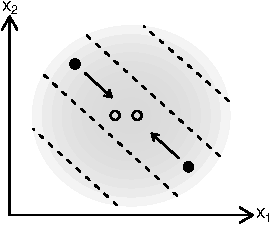
\includegraphics{abdellaoui-borcan-hugh-jones-2021_files/figure-latex/pic-intuition-1} }\subfloat[Caste society: children\label{fig:pic-intuition-2}]{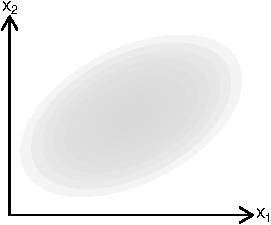
\includegraphics{abdellaoui-borcan-hugh-jones-2021_files/figure-latex/pic-intuition-2} }\newline\subfloat[Egalitarian society ($k = 0$): parents\label{fig:pic-intuition-3}]{\includegraphics{abdellaoui-borcan-hugh-jones-2021_files/figure-latex/pic-intuition-3} }\subfloat[Egalitarian society: children\label{fig:pic-intuition-4}]{\includegraphics{abdellaoui-borcan-hugh-jones-2021_files/figure-latex/pic-intuition-4} }\newline\subfloat[Intermediate society ($0 < k < 1$): parents\label{fig:pic-intuition-5}]{\includegraphics{abdellaoui-borcan-hugh-jones-2021_files/figure-latex/pic-intuition-5} }\subfloat[Intermediate society: children\label{fig:pic-intuition-6}]{\includegraphics{abdellaoui-borcan-hugh-jones-2021_files/figure-latex/pic-intuition-6} }

}

\caption{Theory: shaded area is the population distribution. Dotted lines are attractiveness isoquants. Solid dots are example parents, transparent dots are example children. The right hand side shows the children's generation.}\label{fig:pic-intuition}
\end{figure}

\hypertarget{leftovers}{%
\subsection{Leftovers}\label{leftovers}}

The conditions in Proposition \ref{prop:robustness} are quite plausible. For
\(G\), they require that variance in siblings' scores, on a genetic summary
statistic capturing variation in attractiveness, is either not too large, or
that it is uncorrelated with the parents' scores. Both of these hold for most
polygenic scores, which are additive sums of many small effects of alleles
derived randomly from one or other parent. For \(S\), the conditions would hold,
for example, if \(S\) measures wealth, which is inherited not too unequally
between siblings; or if wealth is inherited unequally but not in a way that
correlates with \(S\) or \(G\).

It is worth considering what kind of social arrangements would \emph{violate}
these conditions. For example, suppose that parents' combined wealth is
inherited by the child with the lowest value of \(g_{c(i)}\). This creates
a negative correlation between \(s_{c(i)}\) and \(g_{c(i)}\).

\hypertarget{discussion}{%
\subsection{Discussion}\label{discussion}}

The ``marriage market'' here is a reduced form mechanism, encompassing
everything that makes a difference to partner choice. For example, if
earned income affects attractiveness in the marriage market, then
society's level of meritocracy in the labour market will correlate with
the value of \(k\): a more meritocratic labour market will allow people
with low social status but high human capital (genetically determined in
part) to earn more, and therefore to match with more attractive
partners.

The contents of both \(S\), social status, and \(G\) -- ``good genes'' in the
marriage market -- are likely to vary across societies. \(S\) could
encompass variables like social class or caste; ethnic identity in
``ranked'' ethnic systems; or in modern societies, SES. Regarding \(G\),
standards of physical attractiveness, and other characteristics which
make someone a ``good match,'' vary both across societies and within a
society over time.

Recent empirical work shows high persistence of SES over time, in particular at
the top. One suggested reason for this is that unmeasured family characteristics
persist along with measured wealth (Clark and Cummins 2015). Our model
captures this idea. For simplicity, let condition \eqref{eq:linearity} hold.
Consider a regression of children's social status on parent's social status:

\[
s_{c(i)} = \alpha + \beta_S s_i + \varepsilon_{c(i)}.
\]

The value of \(\beta_S\) will be less than one, since parents match on
downward sloping isoattractiveness curves: within each curve, relatively
wealthy individuals match with less wealthy individuals on average. Now
consider a regression of child on parent ``attractiveness'' \(A\):

\[
A_{c(i)} = \alpha + \beta_A A_i + \varepsilon_{c(i)}.
\]

Since children are on the same attractiveness curve as both their
parents, \(\beta_A = 1\). Thus, regressions on measured components of
social status will underestimate true persistence over time, embodied in
genetic variation. Indeed, grandparents' social status will
independently predict grandchildren's social status, even after
controlling for parents' social status, because of the unmeasured
pathway via parents' genetics.

The converse also holds: regressions of children's characteristics on their
genetics alone risk overestimating the effect of genetics, by confounding it
with the effects of correlated socio-economic status. Recent work in genetics
has shown just this. Polygenic scores for educational attainment have smaller
effects in between-sibling regressions, where between-family variation in SES is
partialled out and where genes are guaranteed to be randomly allocated, than in
regressions which pool the whole sample (Howe et al. 2021). Parents' genetic
variants which are \emph{not} passed on to children predict children's
characteristics, via environmental effects (Kong et al. 2018).

The model predicts variation in the strength of SGAM. In particular, in
``caste societies'' where there is complete endogamy within social status
groups, there is no scope for SGAM, because marriage partners do not
trade off genetics for social status. The model also assumes that social
status is inherited randomly from one parent, in the same way a genetic
allele is inherited. This assumption can be weakened. For example, if
social status is inherited deterministically from the father, then the
results remain unchanged (for each pair of parents, just assume that one
randomly chosen parent is the father).

In modern societies, both SGAM and meritocratic mobility are likely to
be at play. Genetic variants that cause (e.g.) higher income and wealth
will be inherited along with components of social status such as
inherited wealth. At the same time, higher social status and ``good
genes'' will assort in the marriage market, even if that higher social
status is caused by purely environmental variation. Our empirical
analysis shows this latter process at work.

\hypertarget{data-and-methods}{%
\section{Data and methods}\label{data-and-methods}}

To test for the existence of SGAM, we use data from the UK Biobank, a study of about
500,000 individuals born between 1935 and 1970. The Biobank contains
information on respondents' genetics, derived from DNA microarrays,
along with questionnaire data on health and social outcomes.

The Biobank does not contain explicit information on spouse pairs. We
categorize respondents as pairs if they:

\begin{itemize}
\tightlist
\item
  had the same home postcode on at least one occasion;\footnote{A typical UK postcode contains about 15 properties.}
\item
  both reported the same homeownership/renting status, length of time
  at the address, and number of children;
\item
  attended the same UK Biobank assessment center on the same day;
\item
  both reported living with their spouse (``husband, wife or partner'');
\item
  consisted of one male and one female.
\end{itemize}

We also eliminate all pairs where either spouse appeared more than once
in the data. This leaves a total of 35,682 pairs. Some of
these could be false positives, i.e.~people who are not each others'
spouse but simply live in the same postcode. So, to validate the accuracy of
our pairs, we use genetic relationships. Some respondents in the
Biobank sample have a child who is also in the sample, as inferred from
genetic data. Among our spouse pairs, 511 have a genetic
child of at least one partner in the sample. For 441 of
these, the child is the genetic child of both partners. If this
subsample is representative, then at least
86\% of the pairs who have had a
child, have had a child together. This is a lower bound, because those
who had a child with someone else may also have had a child with the
presumed partner in our data. As a point of comparison, 11\% of families
with dependent children included a stepchild in England and Wales in
2011 (National Statistics 2014).

It is still possible that some pairs in our data may not be actual spouses. In
the appendix, to sign any possible bias in our estimates resulting from this, we
use a dataset of ``known fake'' pairs. We show that estimated coefficients of
interest are closer to zero among these fake pairs than among our candidate
``real pairs.'' Because of this, any fake pairs remaining in our data are likely
to bias our coefficients towards zero.

Our key dependent variable is spouse's \emph{Polygenic Score for Educational
Attainment} (PSEA). A polygenic score is a DNA-derived summary measure
of genetic risk or propensity for a particular outcome, created from
summing small effects of many common genetic variants, known as Single
Nucleotide Polymorphisms (SNPs). We focus on PSEA rather than other
polygenic scores for two reasons. First, educational attainment plays a key role in
human mate search. People are attracted to educated potential partners
(Buss and Barnes 1986; Belot and Francesconi 2013); spouse pairs often have
similar levels of educational attainment, as well as similar PSEA
(Vandenberg 1972; Schwartz and Mare 2005; Greenwood et al. 2014; Hugh-Jones et al. 2016). Second, PSEA predicts a set of important socioeconomic
variables, including not only education but also social and geographic mobility,
IQ, future income and wealth (Belsky et al. 2016; Barth, Papageorge, and Thom 2020; Papageorge and Thom 2020).\footnote{See Papageorge and Thom (2020) for a detailed discussion of polygenic
  scores, aimed at economists.}

We calculate PSEA using per-SNP summary statistics from Lee et al. (2018),
re-estimated excluding UK Biobank participants.\footnote{PSEA was computed by summing the alleles across \textasciitilde1.3 million
  genetic variants weighted by their effect sizes as estimated in
  genome-wide association studies (GWASs) that excluded UK Biobank.
  PSEA was then residualized on the first 100 principal components of
  the SNP array data. Further details can be found in
  Abdellaoui et al. (2019).} We normalize the score to
have mean 0 and variance 1. Because polygenic scores are created from estimates
of many presumably tiny effects, they contain a large amount of noise relative
to the true best estimator that could be derived from genetic data. For
instance, PSEA explains only 11--13\% of variance in educational attainment (out
of sample, Lee et al. 2018), whereas the true proportion explained by genetic
variation -- the heritability -- is estimated from twin studies to be about 40\%
(Branigan, McCallum, and Freese 2013). In addition, polygenic scores are no more guaranteed
to be causal than any other independent variable. For example, social
stratification by descent may lead genes to be associated with educational
attainment even while playing no causal role (Selzam et al. 2019).

Despite these points, PSEA has non-trivial estimated effects on educational
attainment. PSEA correlates with measures of education, including university
attendance and years of full-time education; within-siblings regressions, where
PSEA is randomly assigned by the ``lottery of meiosis,'' confirm this correlation
is at least partly causal (Lee et al. 2018). We recheck these facts within the UK
Biobank sample. In a simple linear regression (N = 408,524) of
university attendance on PSEA, a one-standard-deviation increase in PSEA was
associated with a 9.2 percentage point increase in the
probability of university attendance (\(p < 2 \times 10^{-16}\)). In a
within-siblings regression among genetic full siblings (N =
36,748), the increase was
4.5 (\(p < 2 \times 10^{-16}\)). This suggests
that about half of the raw correlation of PSEA with university attendance is
down to confounds like good environments or parental nurture, while the
remainder is causal. Nevertheless, the causal effect remains substantial: for a
rough comparison, the (ITT) effect on college attendance of the Moving To
Opportunity experiment in the US was 2.5 percentage points (Chetty, Hendren, and Katz 2016).

Figures \ref{fig:pic-basic-corr-uni} and \ref{fig:pic-basic-corr-income}
illustrate the core idea of SGAM within our pair data. The X axis shows a
measure of one partner's socio-economic status: university attendance (Figure
\ref{fig:pic-basic-corr-uni}) or income (Figure
\ref{fig:pic-basic-corr-income}). The Y axis plots the other partner's mean
PSEA. Both males and females who went to university had spouses with higher
PSEA. So did males and females with higher income. Since DNA is inherited, these
people's children will also have higher PSEA.

\begin{figure}
\subfloat[Female PSEA by male educational attainment\label{fig:pic-basic-corr-uni-1}]{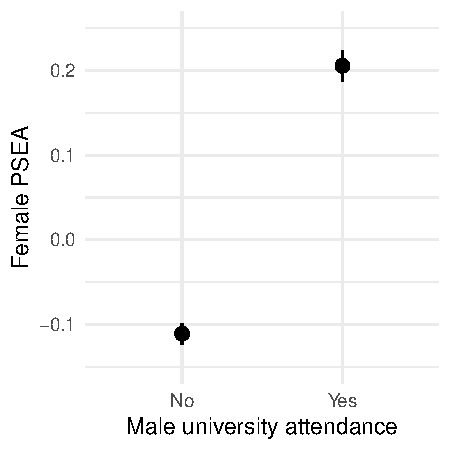
\includegraphics{abdellaoui-borcan-hugh-jones-2021_files/figure-latex/pic-basic-corr-uni-1} }\subfloat[Male PSEA by female educational attainment\label{fig:pic-basic-corr-uni-2}]{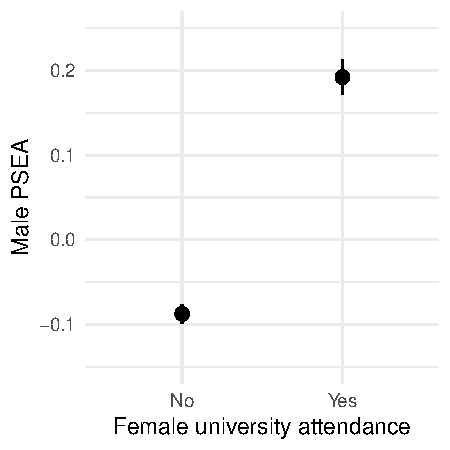
\includegraphics{abdellaoui-borcan-hugh-jones-2021_files/figure-latex/pic-basic-corr-uni-2} }\caption{Spouse PSEA against own university attendance. Lines show 95\% confidence intervals}\label{fig:pic-basic-corr-uni}
\end{figure}

\begin{figure}
\subfloat[Female EA3 by male income\label{fig:pic-basic-corr-income-1}]{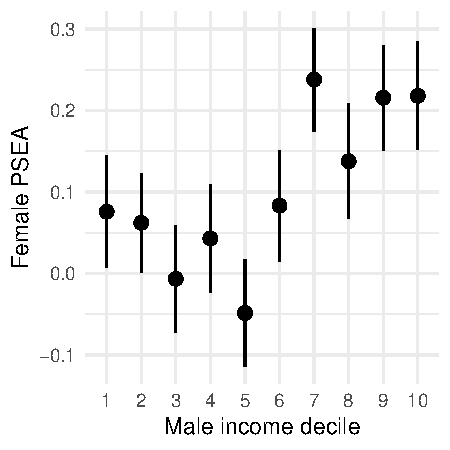
\includegraphics{abdellaoui-borcan-hugh-jones-2021_files/figure-latex/pic-basic-corr-income-1} }\subfloat[Male EA3 by female income\label{fig:pic-basic-corr-income-2}]{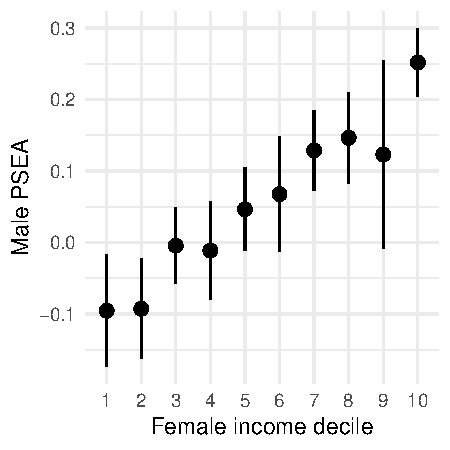
\includegraphics{abdellaoui-borcan-hugh-jones-2021_files/figure-latex/pic-basic-corr-income-2} }\caption{Spouse PSEA against own estimated income in first job. Lines show 95\% confidence intervals}\label{fig:pic-basic-corr-income}
\end{figure}

These figures do not prove that SGAM is taking place. Since an
individual's own PSEA correlates with both their educational attainment,
and their income, both figures could be a result of genetic assortative
mating (GAM) alone (Hugh-Jones et al. 2016). To demonstrate SGAM, we need
a source of social status which is exogenous to genetics. Also, the link
between social status and spouse genetics is likely to be noisy, for
three reasons: first, polygenic scores contain a large amount of error, as
discussed above; second, causal mechanisms behind variation in social status
are likely to be noisy; third, to paraphrase Shakespeare (1595), the
spouse matching process is highly unpredictable. So, we need a large N to
give us sufficient power. This rules out time-limited shocks such as
changes to the school leaving age (Davies et al. 2018).

We use \emph{birth order}. It is known that earlier-born children receive more
parental care and have better life outcomes, including measures of SES such as
educational attainment and occupational status (Lindahl 2008; Booth and Kee 2009; Black, Devereux, and Salvanes 2011). On the other hand, all full siblings have the same \emph{ex ante}
expected genetic endowment from their parents, irrespective of their birth
order. For example, siblings' expected polygenic score is equal to the mean of
their parents' polygenic scores.\footnote{Although genetic variation is randomly assigned to children at
  birth, genetics and birth order could be dependent if parents'
  choice of whether to have more children is endogenous to the genetic
  endowment of their earlier children. We check for this below.
  Isungset et al. (2021) also find that birth order differences in education are
  not genetic.} We can therefore use birth order as a
``shock'' to social status. Despite this language, we do not claim that birth
order is exogenous to all other variables. For example, it naturally correlates
with parental age, and it may also be related to the family's economic position at
the time of birth. We only claim that birth order is exogenous to genetic
variation.

Our main independent variable is respondents' birth order, i.e.~their
number of elder siblings plus one. For controls we use family size, i.e.
respondents' total number of siblings including themselves; month of birth; age
at interview; respondents' own PSEA; and their father's and/or mother's age
at their birth (calculated from parent's current age, only available if
the parent was still alive). For most regressions, we use only
respondents with between 1 and 5 siblings, i.e.~with a family size of
2-6.

To test whether birth order effects are mediated by SES, we use two measures:
income, and university attendance. Income is a direct measure of SES. University
attendance is a predictor of income over the whole life course, and a form of
SES itself. The UK Biobank data only contains a direct measure of current
household income, which is inappropriate for our purposes because it includes
income from both spouses. Instead, we estimate income in the respondent's first
job, from the job's Standard Occupational Classification (SOC) code. We match
this with information on average earnings by SOC from the Annual Survey of Hours
and Earnings 2007 (National Statistics 2007). This data is only available for a subset of
respondents.

\hypertarget{decomposing-the-birth-order-effect-on-spouse-genetics}{%
\subsection{Decomposing the birth order effect on spouse genetics}\label{decomposing-the-birth-order-effect-on-spouse-genetics}}

Ideally, we might prefer to use birth order as an instrument for SES. However,
our measures of social status are noisy and incomplete. For example, we know
whether subjects attended university, but not which university. Birth order
likely affects both measured and unmeasured aspects of SES. So, an instrumental
variables approach would be likely to fall foul of the exclusion restriction.

Instead, we conduct a mediation analysis, following the strategy of
Heckman, Pinto, and Savelyev (2013). We first confirm statistically that birth
order affects our measures of respondents' SES (income and education).
Then, we regress spouse's PSEA on birth order, with and without
controlling for SES. Under the assumption that birth order is exogenous
to own genetics, these regressions identify the effect of birth order,
plus other environmental variables that correlate with it, on own social
status and spouse's genetics. Also, if the estimated effect of birth
order on spouse's PSEA changes when SES is controlled for, that is
evidence that SES mediates the effect of birth order.

Linearizing our model so that \(A(g, s) = (1-k)g + ks\) and applying
\eqref{eq:same-A} shows that:

\[
\frac{d A(g_{p(i)}, s_{p(i)})}{d s_i} = k
\]

We wish to test whether \(k \in (0, 1)\), i.e.~whether SGAM is taking
place. If \(k > 0\) then an increase in \(i\)'s social status \(s_i\) will
increase \(i\)'s attractiveness \(A\); if \(k < 1\) then an increase in \(A\)
will be associated (in expectation) with an increase in \(i\)'s partner's
genetic endowment \(g_{p(i)}\). We therefore wish to estimate the effect
of \(i\)'s status on their partner's genetics, while controlling for \(i\)'s
own genetics \(g_i\). Since measures of genetic endowment, such as PSEA,
are noisy and incomplete, it is not enough to include them as controls in the
regression. Instead, we use birth order as a source of variation in
\(s_i\) which is orthogonal to \(g_i\).

We follow Heckman, Pinto, and Savelyev (2013) to decompose the aggregate treatment
effect into components due to observed and unobserved proximate channels
affected by the treatment. Our aim is to estimate the effect of SES (as
an effect of birth order) on spouse PSEA.

Assume \(B\) is a multivalued variable indicating birth order. Let \(Y_b\) be
the counterfactual outcome (spouse PSEA) for the first-born, second-born etc.
Given \(b\), spouse PSEA is assumed to be independent across observations
conditional on some predetermined controls which are assumed not to be affected
by \(B\).

Let \(\theta_{b}\) be a set of mediators, i.e.~proximate outcomes
determined by \(b\), which account (at least in part) for the \(b\)
treatment effect on spouse PSEA. We can think of \(\theta_{b}\) as all
the effects on attractiveness, such as increments to SES, health,
cognitive and non-cognitive skills, that individuals receive due to
their birth rank. We can split the mediators in \(\theta_b\) into a set \(J_m\) of
measured mediators, including measures of SES, and a set \(J_u\) of
mediators that we cannot measure. We are mainly interested in estimating the effect of
SES on spouse PSEA.

Our linear model is:

\begin{equation}
\label{eq:linear-model}
Y_b = \kappa_b + \sum_{j \in J_m} \alpha_b^j \theta^j_b+\sum_{j \in J_u} \alpha_b^j \theta^j_b + \mathbf{X'} \symbf{\beta_b} + \tilde{\varepsilon}_b = \tau_b + \sum_{j \in J_m} \alpha_b^j \theta^j_b + \mathbf{X'} \symbf{\beta_b} + \varepsilon_b 
\end{equation}

where \(\tilde{\varepsilon}_b\) is a mean-zero residual assumed independent of
\(\theta_b\) and \(\mathbf{X}\);
\(\tau_b = \kappa_b + \sum_{j \in J_u} \alpha_b^j E(\theta^j_b)\); and
\(\varepsilon_b = \tilde{\varepsilon}_b + \sum_{j \in J_u} (\theta^j_b - E(\theta^j_b))\).
We simplify by assuming that \(\beta_b = \beta\)
and \(\alpha_b = \alpha\) for all \(b\), i.e.\textasciitilde that the effects of \(\mathbf{X}\) and
\(\theta_B\) don't differ by birth order.\footnote{Under the assumption that measured and unmeasured mediators are
  uncorrelated, we can test these assumptions by running an OLS regression of an
  extended model \eqref{eq:model-to-estimate} where we interact the measured
  mediators and controls with the treatment \(B\), and test the significance of the
  coefficients on the interaction terms (\(\symbf{\alpha_b}=0\) and
  \(\symbf{\beta_b}=0\)). See Heckman, Pinto, and Savelyev (2013) and Fagereng, Mogstad, and Rønning (2021)
  for details and different applications.} We assume differences in
unmeasured investments due to \(b\) are independent of \(\mathbf{X}\).

We use a linear model for each observed mediator variable:
\begin{equation}
\label{eq:mediator-model}
\theta^j_b=\mu_{0,j}+\textbf{X'}\symbf{\mu_{1,j}}+\mu_{2,j}\cdot b+\eta_j, j \in J_m  
\end{equation}
where \(\eta_j\) is a mean-zero residual. We also assume the treatment-specific intercepts are linear in \(b\):
\begin{equation}
\label{eq:linear-intercept}
\tau_b=\tau_{0}+\tau b.  
\end{equation}

With the simplifying assumptions above and substituting \eqref{eq:mediator-model}-
\eqref{eq:linear-intercept} into \eqref{eq:linear-model} we obtain:
\begin{equation}
\label{eq:simplified-model}
Y_b = \tau_0+\tau b + \sum_{j \in J_m} \alpha^j (\mu_{0,j}+\textbf{X'}\symbf{\mu_{1,j}}+\mu_{2,j}\cdot b+\eta_j) + \mathbf{X'} \symbf{\beta} + \varepsilon_b 
\end{equation}

Using equation \eqref{eq:simplified-model}, we can decompose the average treatment
effect of \(B\) (birth order \(b'\) instead of \(b\)) into the effect of measured mediators \(\theta^j\) and unmeasured mediators on the outcome:

\begin{equation}
\label{eq:decomposition}
E(Y_b' - Y_b) = \tau(b' - b) + \sum_{j \in J_m} \alpha^j E(\theta^j_{b'} - \theta^j_b) \\
=\underbrace{\tau(b' - b)}_{\text{Effect of unmeasured mediators}} + \underbrace{\sum_{j \in J_m} \alpha^j \mu_{2,j} (b' - b)}_{\text{Effect of measured mediators}}
\end{equation}

We are primarily interested in estimating the effect of SES on spouse PSEA,
amongst the measured mediators, and furthermore we would like to measure the
relative importance of SES compared to other factors in predicting spouse PSEA.

We therefore estimate:
\begin{equation}
\label{eq:model-to-estimate}
Y = \tau_0 + \tau B + \sum_{j \in J_m} \alpha^j \theta^j_b + \mathbf{X'} \symbf{\beta} + \varepsilon
\end{equation}

Estimating the above by OLS will generate unbiased estimates of
\(\alpha^j\) if \(\theta^j\) is measured without error and is
uncorrelated with the error term \(\varepsilon\). Since
\(\varepsilon\) contains both individual disturbances and differences
in unmeasured investments due to birth order, there are two identifying assumptions that need to hold for unbiased OLS estimates: (a) the measured investments
(specifically SES) should be independent of unmeasured investments
generated by birth order. Failing this, the estimates of \(\alpha^j\) will be
conflated with the effects of unmeasured investments. Second, (b) the measured
investments should be uncorrelated with other shocks \(\tilde{\varepsilon}_b\).

By running a least square regression of \eqref{eq:model-to-estimate}, we can
estimate \(\tau\) and \(\alpha^j\). If assumption (a) holds, the part of the
birth order treatment effect on spouse PSEA that is due to measured mediators,
including SES, can be constructed using the estimated \(\alpha^j\) and the effects
of birth order on measured mediators. We can estimate these effects in a second
step, from OLS regressions based on equation \eqref{eq:mediator-model} for each
measured mediator (in particular university attendance and income) on \(X\) and
\(B\). The part of the birth order effect that is due to university attendance (or
income) on spouse PSEA will be the coefficient of university (income) in the
regression of spouse PSEA in equation \eqref{eq:model-to-estimate} multiplied by
the coefficient of birth order from equation \eqref{eq:mediator-model}.

\hypertarget{results}{%
\section{Results}\label{results}}

 
  \providecommand{\huxb}[2]{\arrayrulecolor[RGB]{#1}\global\arrayrulewidth=#2pt}
  \providecommand{\huxvb}[2]{\color[RGB]{#1}\vrule width #2pt}
  \providecommand{\huxtpad}[1]{\rule{0pt}{#1}}
  \providecommand{\huxbpad}[1]{\rule[-#1]{0pt}{#1}}

\begin{table}[ht]
\begin{centerbox}
\begin{threeparttable}
\captionsetup{justification=centering,singlelinecheck=off}
\caption{\label{tab:tbl-bo-first-stage} Regressions of variables on birth order}
 \setlength{\tabcolsep}{0pt}
\begin{tabularx}{0.9\textwidth}{p{0.18\textwidth} p{0.18\textwidth} p{0.18\textwidth} p{0.18\textwidth} p{0.18\textwidth}}


\hhline{>{\huxb{0, 0, 0}{0.8}}->{\huxb{0, 0, 0}{0.8}}->{\huxb{0, 0, 0}{0.8}}->{\huxb{0, 0, 0}{0.8}}->{\huxb{0, 0, 0}{0.8}}-}
\arrayrulecolor{black}

\multicolumn{1}{!{\huxvb{0, 0, 0}{0}}p{0.18\textwidth}!{\huxvb{0, 0, 0}{0}}}{\hspace{6pt}\parbox[b]{0.18\textwidth-6pt-6pt}{\huxtpad{6pt + 1em}\centering \huxbpad{6pt}}} &
\multicolumn{1}{p{0.18\textwidth}!{\huxvb{0, 0, 0}{0}}}{\hspace{6pt}\parbox[b]{0.18\textwidth-6pt-6pt}{\huxtpad{6pt + 1em}\centering University\huxbpad{6pt}}} &
\multicolumn{1}{p{0.18\textwidth}!{\huxvb{0, 0, 0}{0}}}{\hspace{6pt}\parbox[b]{0.18\textwidth-6pt-6pt}{\huxtpad{6pt + 1em}\centering Income\huxbpad{6pt}}} &
\multicolumn{1}{p{0.18\textwidth}!{\huxvb{0, 0, 0}{0}}}{\hspace{6pt}\parbox[b]{0.18\textwidth-6pt-6pt}{\huxtpad{6pt + 1em}\centering Fluid IQ\huxbpad{6pt}}} &
\multicolumn{1}{p{0.18\textwidth}!{\huxvb{0, 0, 0}{0}}}{\hspace{6pt}\parbox[b]{0.18\textwidth-6pt-6pt}{\huxtpad{6pt + 1em}\centering Height\huxbpad{6pt}}} \tabularnewline[-0.5pt]


\hhline{>{\huxb{255, 255, 255}{0.4}}->{\huxb{0, 0, 0}{0.4}}->{\huxb{0, 0, 0}{0.4}}->{\huxb{0, 0, 0}{0.4}}->{\huxb{0, 0, 0}{0.4}}-}
\arrayrulecolor{black}

\multicolumn{1}{!{\huxvb{0, 0, 0}{0}}p{0.18\textwidth}!{\huxvb{0, 0, 0}{0}}}{\hspace{6pt}\parbox[b]{0.18\textwidth-6pt-6pt}{\huxtpad{6pt + 1em}\raggedright Birth order\huxbpad{6pt}}} &
\multicolumn{1}{p{0.18\textwidth}!{\huxvb{0, 0, 0}{0}}}{\hspace{6pt}\parbox[b]{0.18\textwidth-6pt-6pt}{\huxtpad{6pt + 1em}\raggedleft $-$0.0789 ***\huxbpad{6pt}}} &
\multicolumn{1}{p{0.18\textwidth}!{\huxvb{0, 0, 0}{0}}}{\hspace{6pt}\parbox[b]{0.18\textwidth-6pt-6pt}{\huxtpad{6pt + 1em}\raggedleft $-$1.0882 *~~\huxbpad{6pt}}} &
\multicolumn{1}{p{0.18\textwidth}!{\huxvb{0, 0, 0}{0}}}{\hspace{6pt}\parbox[b]{0.18\textwidth-6pt-6pt}{\huxtpad{6pt + 1em}\raggedleft $-$0.2718 ***\huxbpad{6pt}}} &
\multicolumn{1}{p{0.18\textwidth}!{\huxvb{0, 0, 0}{0}}}{\hspace{6pt}\parbox[b]{0.18\textwidth-6pt-6pt}{\huxtpad{6pt + 1em}\raggedleft $-$0.7051 ***\huxbpad{6pt}}} \tabularnewline[-0.5pt]


\hhline{}
\arrayrulecolor{black}

\multicolumn{1}{!{\huxvb{0, 0, 0}{0}}p{0.18\textwidth}!{\huxvb{0, 0, 0}{0}}}{\hspace{6pt}\parbox[b]{0.18\textwidth-6pt-6pt}{\huxtpad{6pt + 1em}\raggedright \huxbpad{6pt}}} &
\multicolumn{1}{p{0.18\textwidth}!{\huxvb{0, 0, 0}{0}}}{\hspace{6pt}\parbox[b]{0.18\textwidth-6pt-6pt}{\huxtpad{6pt + 1em}\raggedleft (0.0067)~~~\huxbpad{6pt}}} &
\multicolumn{1}{p{0.18\textwidth}!{\huxvb{0, 0, 0}{0}}}{\hspace{6pt}\parbox[b]{0.18\textwidth-6pt-6pt}{\huxtpad{6pt + 1em}\raggedleft (0.4264)~~~\huxbpad{6pt}}} &
\multicolumn{1}{p{0.18\textwidth}!{\huxvb{0, 0, 0}{0}}}{\hspace{6pt}\parbox[b]{0.18\textwidth-6pt-6pt}{\huxtpad{6pt + 1em}\raggedleft (0.0304)~~~\huxbpad{6pt}}} &
\multicolumn{1}{p{0.18\textwidth}!{\huxvb{0, 0, 0}{0}}}{\hspace{6pt}\parbox[b]{0.18\textwidth-6pt-6pt}{\huxtpad{6pt + 1em}\raggedleft (0.1353)~~~\huxbpad{6pt}}} \tabularnewline[-0.5pt]


\hhline{}
\arrayrulecolor{black}

\multicolumn{1}{!{\huxvb{0, 0, 0}{0}}p{0.18\textwidth}!{\huxvb{0, 0, 0}{0}}}{\hspace{6pt}\parbox[b]{0.18\textwidth-6pt-6pt}{\huxtpad{6pt + 1em}\raggedright PSEA\huxbpad{6pt}}} &
\multicolumn{1}{p{0.18\textwidth}!{\huxvb{0, 0, 0}{0}}}{\hspace{6pt}\parbox[b]{0.18\textwidth-6pt-6pt}{\huxtpad{6pt + 1em}\raggedleft 0.0890 ***\huxbpad{6pt}}} &
\multicolumn{1}{p{0.18\textwidth}!{\huxvb{0, 0, 0}{0}}}{\hspace{6pt}\parbox[b]{0.18\textwidth-6pt-6pt}{\huxtpad{6pt + 1em}\raggedleft 1.5211 ***\huxbpad{6pt}}} &
\multicolumn{1}{p{0.18\textwidth}!{\huxvb{0, 0, 0}{0}}}{\hspace{6pt}\parbox[b]{0.18\textwidth-6pt-6pt}{\huxtpad{6pt + 1em}\raggedleft 0.3172 ***\huxbpad{6pt}}} &
\multicolumn{1}{p{0.18\textwidth}!{\huxvb{0, 0, 0}{0}}}{\hspace{6pt}\parbox[b]{0.18\textwidth-6pt-6pt}{\huxtpad{6pt + 1em}\raggedleft 0.1921 *~~\huxbpad{6pt}}} \tabularnewline[-0.5pt]


\hhline{}
\arrayrulecolor{black}

\multicolumn{1}{!{\huxvb{0, 0, 0}{0}}p{0.18\textwidth}!{\huxvb{0, 0, 0}{0}}}{\hspace{6pt}\parbox[b]{0.18\textwidth-6pt-6pt}{\huxtpad{6pt + 1em}\raggedright \huxbpad{6pt}}} &
\multicolumn{1}{p{0.18\textwidth}!{\huxvb{0, 0, 0}{0}}}{\hspace{6pt}\parbox[b]{0.18\textwidth-6pt-6pt}{\huxtpad{6pt + 1em}\raggedleft (0.0046)~~~\huxbpad{6pt}}} &
\multicolumn{1}{p{0.18\textwidth}!{\huxvb{0, 0, 0}{0}}}{\hspace{6pt}\parbox[b]{0.18\textwidth-6pt-6pt}{\huxtpad{6pt + 1em}\raggedleft (0.3296)~~~\huxbpad{6pt}}} &
\multicolumn{1}{p{0.18\textwidth}!{\huxvb{0, 0, 0}{0}}}{\hspace{6pt}\parbox[b]{0.18\textwidth-6pt-6pt}{\huxtpad{6pt + 1em}\raggedleft (0.0200)~~~\huxbpad{6pt}}} &
\multicolumn{1}{p{0.18\textwidth}!{\huxvb{0, 0, 0}{0}}}{\hspace{6pt}\parbox[b]{0.18\textwidth-6pt-6pt}{\huxtpad{6pt + 1em}\raggedleft (0.0919)~~~\huxbpad{6pt}}} \tabularnewline[-0.5pt]


\hhline{}
\arrayrulecolor{black}

\multicolumn{1}{!{\huxvb{0, 0, 0}{0}}p{0.18\textwidth}!{\huxvb{0, 0, 0}{0}}}{\hspace{6pt}\parbox[b]{0.18\textwidth-6pt-6pt}{\huxtpad{6pt + 1em}\raggedright Parents' age at birth\huxbpad{6pt}}} &
\multicolumn{1}{p{0.18\textwidth}!{\huxvb{0, 0, 0}{0}}}{\hspace{6pt}\parbox[b]{0.18\textwidth-6pt-6pt}{\huxtpad{6pt + 1em}\raggedleft 0.0164 ***\huxbpad{6pt}}} &
\multicolumn{1}{p{0.18\textwidth}!{\huxvb{0, 0, 0}{0}}}{\hspace{6pt}\parbox[b]{0.18\textwidth-6pt-6pt}{\huxtpad{6pt + 1em}\raggedleft 0.2631 ***\huxbpad{6pt}}} &
\multicolumn{1}{p{0.18\textwidth}!{\huxvb{0, 0, 0}{0}}}{\hspace{6pt}\parbox[b]{0.18\textwidth-6pt-6pt}{\huxtpad{6pt + 1em}\raggedleft 0.0588 ***\huxbpad{6pt}}} &
\multicolumn{1}{p{0.18\textwidth}!{\huxvb{0, 0, 0}{0}}}{\hspace{6pt}\parbox[b]{0.18\textwidth-6pt-6pt}{\huxtpad{6pt + 1em}\raggedleft 0.1515 ***\huxbpad{6pt}}} \tabularnewline[-0.5pt]


\hhline{}
\arrayrulecolor{black}

\multicolumn{1}{!{\huxvb{0, 0, 0}{0}}p{0.18\textwidth}!{\huxvb{0, 0, 0}{0}}}{\hspace{6pt}\parbox[b]{0.18\textwidth-6pt-6pt}{\huxtpad{6pt + 1em}\raggedright \huxbpad{6pt}}} &
\multicolumn{1}{p{0.18\textwidth}!{\huxvb{0, 0, 0}{0}}}{\hspace{6pt}\parbox[b]{0.18\textwidth-6pt-6pt}{\huxtpad{6pt + 1em}\raggedleft (0.0012)~~~\huxbpad{6pt}}} &
\multicolumn{1}{p{0.18\textwidth}!{\huxvb{0, 0, 0}{0}}}{\hspace{6pt}\parbox[b]{0.18\textwidth-6pt-6pt}{\huxtpad{6pt + 1em}\raggedleft (0.0721)~~~\huxbpad{6pt}}} &
\multicolumn{1}{p{0.18\textwidth}!{\huxvb{0, 0, 0}{0}}}{\hspace{6pt}\parbox[b]{0.18\textwidth-6pt-6pt}{\huxtpad{6pt + 1em}\raggedleft (0.0053)~~~\huxbpad{6pt}}} &
\multicolumn{1}{p{0.18\textwidth}!{\huxvb{0, 0, 0}{0}}}{\hspace{6pt}\parbox[b]{0.18\textwidth-6pt-6pt}{\huxtpad{6pt + 1em}\raggedleft (0.0241)~~~\huxbpad{6pt}}} \tabularnewline[-0.5pt]


\hhline{>{\huxb{255, 255, 255}{0.4}}->{\huxb{0, 0, 0}{0.4}}->{\huxb{0, 0, 0}{0.4}}->{\huxb{0, 0, 0}{0.4}}->{\huxb{0, 0, 0}{0.4}}-}
\arrayrulecolor{black}

\multicolumn{1}{!{\huxvb{0, 0, 0}{0}}p{0.18\textwidth}!{\huxvb{0, 0, 0}{0}}}{\hspace{6pt}\parbox[b]{0.18\textwidth-6pt-6pt}{\huxtpad{6pt + 1em}\raggedright Family size dummies\huxbpad{6pt}}} &
\multicolumn{1}{p{0.18\textwidth}!{\huxvb{0, 0, 0}{0}}}{\hspace{6pt}\parbox[b]{0.18\textwidth-6pt-6pt}{\huxtpad{6pt + 1em}\centering Yes\huxbpad{6pt}}} &
\multicolumn{1}{p{0.18\textwidth}!{\huxvb{0, 0, 0}{0}}}{\hspace{6pt}\parbox[b]{0.18\textwidth-6pt-6pt}{\huxtpad{6pt + 1em}\centering Yes\huxbpad{6pt}}} &
\multicolumn{1}{p{0.18\textwidth}!{\huxvb{0, 0, 0}{0}}}{\hspace{6pt}\parbox[b]{0.18\textwidth-6pt-6pt}{\huxtpad{6pt + 1em}\centering Yes\huxbpad{6pt}}} &
\multicolumn{1}{p{0.18\textwidth}!{\huxvb{0, 0, 0}{0}}}{\hspace{6pt}\parbox[b]{0.18\textwidth-6pt-6pt}{\huxtpad{6pt + 1em}\centering Yes\huxbpad{6pt}}} \tabularnewline[-0.5pt]


\hhline{}
\arrayrulecolor{black}

\multicolumn{1}{!{\huxvb{0, 0, 0}{0}}p{0.18\textwidth}!{\huxvb{0, 0, 0}{0}}}{\hspace{6pt}\parbox[b]{0.18\textwidth-6pt-6pt}{\huxtpad{6pt + 1em}\raggedright Birth month dummies\huxbpad{6pt}}} &
\multicolumn{1}{p{0.18\textwidth}!{\huxvb{0, 0, 0}{0}}}{\hspace{6pt}\parbox[b]{0.18\textwidth-6pt-6pt}{\huxtpad{6pt + 1em}\centering Yes\huxbpad{6pt}}} &
\multicolumn{1}{p{0.18\textwidth}!{\huxvb{0, 0, 0}{0}}}{\hspace{6pt}\parbox[b]{0.18\textwidth-6pt-6pt}{\huxtpad{6pt + 1em}\centering Yes\huxbpad{6pt}}} &
\multicolumn{1}{p{0.18\textwidth}!{\huxvb{0, 0, 0}{0}}}{\hspace{6pt}\parbox[b]{0.18\textwidth-6pt-6pt}{\huxtpad{6pt + 1em}\centering Yes\huxbpad{6pt}}} &
\multicolumn{1}{p{0.18\textwidth}!{\huxvb{0, 0, 0}{0}}}{\hspace{6pt}\parbox[b]{0.18\textwidth-6pt-6pt}{\huxtpad{6pt + 1em}\centering Yes\huxbpad{6pt}}} \tabularnewline[-0.5pt]


\hhline{}
\arrayrulecolor{black}

\multicolumn{1}{!{\huxvb{0, 0, 0}{0}}p{0.18\textwidth}!{\huxvb{0, 0, 0}{0}}}{\hspace{6pt}\parbox[b]{0.18\textwidth-6pt-6pt}{\huxtpad{6pt + 1em}\raggedright Birth year dummies\huxbpad{6pt}}} &
\multicolumn{1}{p{0.18\textwidth}!{\huxvb{0, 0, 0}{0}}}{\hspace{6pt}\parbox[b]{0.18\textwidth-6pt-6pt}{\huxtpad{6pt + 1em}\centering Yes\huxbpad{6pt}}} &
\multicolumn{1}{p{0.18\textwidth}!{\huxvb{0, 0, 0}{0}}}{\hspace{6pt}\parbox[b]{0.18\textwidth-6pt-6pt}{\huxtpad{6pt + 1em}\centering Yes\huxbpad{6pt}}} &
\multicolumn{1}{p{0.18\textwidth}!{\huxvb{0, 0, 0}{0}}}{\hspace{6pt}\parbox[b]{0.18\textwidth-6pt-6pt}{\huxtpad{6pt + 1em}\centering Yes\huxbpad{6pt}}} &
\multicolumn{1}{p{0.18\textwidth}!{\huxvb{0, 0, 0}{0}}}{\hspace{6pt}\parbox[b]{0.18\textwidth-6pt-6pt}{\huxtpad{6pt + 1em}\centering Yes\huxbpad{6pt}}} \tabularnewline[-0.5pt]


\hhline{>{\huxb{255, 255, 255}{0.4}}->{\huxb{0, 0, 0}{0.4}}->{\huxb{0, 0, 0}{0.4}}->{\huxb{0, 0, 0}{0.4}}->{\huxb{0, 0, 0}{0.4}}-}
\arrayrulecolor{black}

\multicolumn{1}{!{\huxvb{0, 0, 0}{0}}p{0.18\textwidth}!{\huxvb{0, 0, 0}{0}}}{\hspace{6pt}\parbox[b]{0.18\textwidth-6pt-6pt}{\huxtpad{6pt + 1em}\raggedright N\huxbpad{6pt}}} &
\multicolumn{1}{p{0.18\textwidth}!{\huxvb{0, 0, 0}{0}}}{\hspace{6pt}\parbox[b]{0.18\textwidth-6pt-6pt}{\huxtpad{6pt + 1em}\raggedleft 10243~~~~~~~~~\huxbpad{6pt}}} &
\multicolumn{1}{p{0.18\textwidth}!{\huxvb{0, 0, 0}{0}}}{\hspace{6pt}\parbox[b]{0.18\textwidth-6pt-6pt}{\huxtpad{6pt + 1em}\raggedleft 3419~~~~~~~~~\huxbpad{6pt}}} &
\multicolumn{1}{p{0.18\textwidth}!{\huxvb{0, 0, 0}{0}}}{\hspace{6pt}\parbox[b]{0.18\textwidth-6pt-6pt}{\huxtpad{6pt + 1em}\raggedleft 10243~~~~~~~~~\huxbpad{6pt}}} &
\multicolumn{1}{p{0.18\textwidth}!{\huxvb{0, 0, 0}{0}}}{\hspace{6pt}\parbox[b]{0.18\textwidth-6pt-6pt}{\huxtpad{6pt + 1em}\raggedleft 10243~~~~~~~~~\huxbpad{6pt}}} \tabularnewline[-0.5pt]


\hhline{}
\arrayrulecolor{black}

\multicolumn{1}{!{\huxvb{0, 0, 0}{0}}p{0.18\textwidth}!{\huxvb{0, 0, 0}{0}}}{\hspace{6pt}\parbox[b]{0.18\textwidth-6pt-6pt}{\huxtpad{6pt + 1em}\raggedright R2\huxbpad{6pt}}} &
\multicolumn{1}{p{0.18\textwidth}!{\huxvb{0, 0, 0}{0}}}{\hspace{6pt}\parbox[b]{0.18\textwidth-6pt-6pt}{\huxtpad{6pt + 1em}\raggedleft 0.074~~~~~\huxbpad{6pt}}} &
\multicolumn{1}{p{0.18\textwidth}!{\huxvb{0, 0, 0}{0}}}{\hspace{6pt}\parbox[b]{0.18\textwidth-6pt-6pt}{\huxtpad{6pt + 1em}\raggedleft 0.026~~~~~\huxbpad{6pt}}} &
\multicolumn{1}{p{0.18\textwidth}!{\huxvb{0, 0, 0}{0}}}{\hspace{6pt}\parbox[b]{0.18\textwidth-6pt-6pt}{\huxtpad{6pt + 1em}\raggedleft 0.058~~~~~\huxbpad{6pt}}} &
\multicolumn{1}{p{0.18\textwidth}!{\huxvb{0, 0, 0}{0}}}{\hspace{6pt}\parbox[b]{0.18\textwidth-6pt-6pt}{\huxtpad{6pt + 1em}\raggedleft 0.017~~~~~\huxbpad{6pt}}} \tabularnewline[-0.5pt]


\hhline{>{\huxb{0, 0, 0}{0.8}}->{\huxb{0, 0, 0}{0.8}}->{\huxb{0, 0, 0}{0.8}}->{\huxb{0, 0, 0}{0.8}}->{\huxb{0, 0, 0}{0.8}}-}
\arrayrulecolor{black}

\multicolumn{5}{!{\huxvb{0, 0, 0}{0}}p{0.9\textwidth+8\tabcolsep}!{\huxvb{0, 0, 0}{0}}}{\hspace{6pt}\parbox[b]{0.9\textwidth+8\tabcolsep-6pt-6pt}{\huxtpad{6pt + 1em}\raggedright Estimates from OLS regressions with the  mediators (university attendance, income, fluid IQ and height) as dependent variables, and own birth order as the main independent variable. PSEA is the polygenic score for educational attainment, which is normalized with mean 0 and standard deviation 1. We include parents' age at birth (the mean of parents' ages) and further controls to ensure the balance of covariates across birth order. All data is from the UK Biobank for a sample of UK individuals born between 1935 and 1970.  *** p $<$ 0.001;  ** p $<$ 0.01;  * p $<$ 0.05;  + p $<$ 0.1. Standard errors: robust.\huxbpad{6pt}}} \tabularnewline[-0.5pt]


\hhline{}
\arrayrulecolor{black}
\end{tabularx}
\end{threeparttable}\par\end{centerbox}

\end{table}
 

We first regress our measures of socio-economic status, university attendance
and income from first job, on birth order in our sample. We also do the same for
two non-SES mediators that could be affected by birth order: fluid IQ and height.
We control for respondent's own PSEA and their parents' age at birth (see below).
Table \ref{tab:tbl-bo-first-stage} shows that birth order significantly
predicts all these variables. Effect sizes are quite substantial: a single extra
elder sibling reduces the chance of attending university by about
7.9 percentage points, income by about
£1,088, fluid IQ by about
0.27 points on a 13 point test, and height by about
0.71 centimeters.

Next we run regressions of spouse PSEA on birth order, within our
dataset of spouse pairs. Table \ref{tab:tbl-bo-psea-basic} reports the
results. Column 1 controls only for family size (using dummies). As
expected, higher birth order is negatively associated with spouse's
PSEA, though the estimated effect size is small and insignificant.
Column 2 includes the respondent's own PSEA, as well as dummies for birth year
to control for cohort effects, and dummies for birth month to control for
seasonality effects. The effect size of birth order is not much changed.

Column 3 includes parents' age at birth. Within a family, later children
have older parents by definition. Older parents have more life
experience and may have higher income, which would presumably help later
children.\footnote{We often only have data only for one parent. We use this, or take the mean
  if we have both. There are also potential
  genetic effects from parental age, though recent research has rejected these
  in favour of ``social'' explanations (Kristensen and Bjerkedal 2007; Black, Devereux, and Salvanes 2011).
  Cochran and Harpending (2013) report that mutational load is approximately
  linear in father's age, while it is constant in mother's age. We
  observe very similar results if we control only for father's age at
  respondent's birth.} Including parents' age means we can separate the effect
of parental age from birth order. This reduces the N by a lot, since
only respondents with a live parent reported the necessary data. However,
the effect of birth order jumps in size and becomes significant at the 5 per
cent level. Meanwhile, parents' age has a
positive effect. This suggests that estimates in columns 1-2 mixed two
opposite-signed effects: having older parents versus being later in
birth order.

 
  \providecommand{\huxb}[2]{\arrayrulecolor[RGB]{#1}\global\arrayrulewidth=#2pt}
  \providecommand{\huxvb}[2]{\color[RGB]{#1}\vrule width #2pt}
  \providecommand{\huxtpad}[1]{\rule{0pt}{#1}}
  \providecommand{\huxbpad}[1]{\rule[-#1]{0pt}{#1}}

\begin{table}[ht]
\begin{centerbox}
\begin{threeparttable}
\captionsetup{justification=centering,singlelinecheck=off}
\caption{\label{tab:tbl-bo-psea-basic} Regressions of spouse PSEA on birth order}
 \setlength{\tabcolsep}{0pt}
\begin{tabularx}{0.8\textwidth}{p{0.2\textwidth} p{0.2\textwidth} p{0.2\textwidth} p{0.2\textwidth}}


\hhline{>{\huxb{0, 0, 0}{0.8}}->{\huxb{0, 0, 0}{0.8}}->{\huxb{0, 0, 0}{0.8}}->{\huxb{0, 0, 0}{0.8}}-}
\arrayrulecolor{black}

\multicolumn{1}{!{\huxvb{0, 0, 0}{0}}p{0.2\textwidth}!{\huxvb{0, 0, 0}{0}}}{\hspace{6pt}\parbox[b]{0.2\textwidth-6pt-6pt}{\huxtpad{6pt + 1em}\centering \huxbpad{6pt}}} &
\multicolumn{1}{p{0.2\textwidth}!{\huxvb{0, 0, 0}{0}}}{\hspace{6pt}\parbox[b]{0.2\textwidth-6pt-6pt}{\huxtpad{6pt + 1em}\centering (1)\huxbpad{6pt}}} &
\multicolumn{1}{p{0.2\textwidth}!{\huxvb{0, 0, 0}{0}}}{\hspace{6pt}\parbox[b]{0.2\textwidth-6pt-6pt}{\huxtpad{6pt + 1em}\centering (2)\huxbpad{6pt}}} &
\multicolumn{1}{p{0.2\textwidth}!{\huxvb{0, 0, 0}{0}}}{\hspace{6pt}\parbox[b]{0.2\textwidth-6pt-6pt}{\huxtpad{6pt + 1em}\centering (3)\huxbpad{6pt}}} \tabularnewline[-0.5pt]


\hhline{>{\huxb{255, 255, 255}{0.4}}->{\huxb{0, 0, 0}{0.4}}->{\huxb{0, 0, 0}{0.4}}->{\huxb{0, 0, 0}{0.4}}-}
\arrayrulecolor{black}

\multicolumn{1}{!{\huxvb{0, 0, 0}{0}}p{0.2\textwidth}!{\huxvb{0, 0, 0}{0}}}{\hspace{6pt}\parbox[b]{0.2\textwidth-6pt-6pt}{\huxtpad{6pt + 1em}\raggedright Birth order\huxbpad{6pt}}} &
\multicolumn{1}{p{0.2\textwidth}!{\huxvb{0, 0, 0}{0}}}{\hspace{6pt}\parbox[b]{0.2\textwidth-6pt-6pt}{\huxtpad{6pt + 1em}\raggedleft $-$0.0099~\huxbpad{6pt}}} &
\multicolumn{1}{p{0.2\textwidth}!{\huxvb{0, 0, 0}{0}}}{\hspace{6pt}\parbox[b]{0.2\textwidth-6pt-6pt}{\huxtpad{6pt + 1em}\raggedleft $-$0.0079~~~~\huxbpad{6pt}}} &
\multicolumn{1}{p{0.2\textwidth}!{\huxvb{0, 0, 0}{0}}}{\hspace{6pt}\parbox[b]{0.2\textwidth-6pt-6pt}{\huxtpad{6pt + 1em}\raggedleft $-$0.0312 *~~\huxbpad{6pt}}} \tabularnewline[-0.5pt]


\hhline{}
\arrayrulecolor{black}

\multicolumn{1}{!{\huxvb{0, 0, 0}{0}}p{0.2\textwidth}!{\huxvb{0, 0, 0}{0}}}{\hspace{6pt}\parbox[b]{0.2\textwidth-6pt-6pt}{\huxtpad{6pt + 1em}\raggedright \huxbpad{6pt}}} &
\multicolumn{1}{p{0.2\textwidth}!{\huxvb{0, 0, 0}{0}}}{\hspace{6pt}\parbox[b]{0.2\textwidth-6pt-6pt}{\huxtpad{6pt + 1em}\raggedleft (0.0074)\huxbpad{6pt}}} &
\multicolumn{1}{p{0.2\textwidth}!{\huxvb{0, 0, 0}{0}}}{\hspace{6pt}\parbox[b]{0.2\textwidth-6pt-6pt}{\huxtpad{6pt + 1em}\raggedleft (0.0074)~~~\huxbpad{6pt}}} &
\multicolumn{1}{p{0.2\textwidth}!{\huxvb{0, 0, 0}{0}}}{\hspace{6pt}\parbox[b]{0.2\textwidth-6pt-6pt}{\huxtpad{6pt + 1em}\raggedleft (0.0146)~~~\huxbpad{6pt}}} \tabularnewline[-0.5pt]


\hhline{}
\arrayrulecolor{black}

\multicolumn{1}{!{\huxvb{0, 0, 0}{0}}p{0.2\textwidth}!{\huxvb{0, 0, 0}{0}}}{\hspace{6pt}\parbox[b]{0.2\textwidth-6pt-6pt}{\huxtpad{6pt + 1em}\raggedright Own PSEA\huxbpad{6pt}}} &
\multicolumn{1}{p{0.2\textwidth}!{\huxvb{0, 0, 0}{0}}}{\hspace{6pt}\parbox[b]{0.2\textwidth-6pt-6pt}{\huxtpad{6pt + 1em}\raggedleft ~~~~~~\huxbpad{6pt}}} &
\multicolumn{1}{p{0.2\textwidth}!{\huxvb{0, 0, 0}{0}}}{\hspace{6pt}\parbox[b]{0.2\textwidth-6pt-6pt}{\huxtpad{6pt + 1em}\raggedleft 0.0651 ***\huxbpad{6pt}}} &
\multicolumn{1}{p{0.2\textwidth}!{\huxvb{0, 0, 0}{0}}}{\hspace{6pt}\parbox[b]{0.2\textwidth-6pt-6pt}{\huxtpad{6pt + 1em}\raggedleft 0.0583 ***\huxbpad{6pt}}} \tabularnewline[-0.5pt]


\hhline{}
\arrayrulecolor{black}

\multicolumn{1}{!{\huxvb{0, 0, 0}{0}}p{0.2\textwidth}!{\huxvb{0, 0, 0}{0}}}{\hspace{6pt}\parbox[b]{0.2\textwidth-6pt-6pt}{\huxtpad{6pt + 1em}\raggedright \huxbpad{6pt}}} &
\multicolumn{1}{p{0.2\textwidth}!{\huxvb{0, 0, 0}{0}}}{\hspace{6pt}\parbox[b]{0.2\textwidth-6pt-6pt}{\huxtpad{6pt + 1em}\raggedleft ~~~~~~\huxbpad{6pt}}} &
\multicolumn{1}{p{0.2\textwidth}!{\huxvb{0, 0, 0}{0}}}{\hspace{6pt}\parbox[b]{0.2\textwidth-6pt-6pt}{\huxtpad{6pt + 1em}\raggedleft (0.0065)~~~\huxbpad{6pt}}} &
\multicolumn{1}{p{0.2\textwidth}!{\huxvb{0, 0, 0}{0}}}{\hspace{6pt}\parbox[b]{0.2\textwidth-6pt-6pt}{\huxtpad{6pt + 1em}\raggedleft (0.0100)~~~\huxbpad{6pt}}} \tabularnewline[-0.5pt]


\hhline{}
\arrayrulecolor{black}

\multicolumn{1}{!{\huxvb{0, 0, 0}{0}}p{0.2\textwidth}!{\huxvb{0, 0, 0}{0}}}{\hspace{6pt}\parbox[b]{0.2\textwidth-6pt-6pt}{\huxtpad{6pt + 1em}\raggedright Parents' age at birth\huxbpad{6pt}}} &
\multicolumn{1}{p{0.2\textwidth}!{\huxvb{0, 0, 0}{0}}}{\hspace{6pt}\parbox[b]{0.2\textwidth-6pt-6pt}{\huxtpad{6pt + 1em}\raggedleft ~~~~~~\huxbpad{6pt}}} &
\multicolumn{1}{p{0.2\textwidth}!{\huxvb{0, 0, 0}{0}}}{\hspace{6pt}\parbox[b]{0.2\textwidth-6pt-6pt}{\huxtpad{6pt + 1em}\raggedleft ~~~~~~~~~\huxbpad{6pt}}} &
\multicolumn{1}{p{0.2\textwidth}!{\huxvb{0, 0, 0}{0}}}{\hspace{6pt}\parbox[b]{0.2\textwidth-6pt-6pt}{\huxtpad{6pt + 1em}\raggedleft 0.0113 ***\huxbpad{6pt}}} \tabularnewline[-0.5pt]


\hhline{}
\arrayrulecolor{black}

\multicolumn{1}{!{\huxvb{0, 0, 0}{0}}p{0.2\textwidth}!{\huxvb{0, 0, 0}{0}}}{\hspace{6pt}\parbox[b]{0.2\textwidth-6pt-6pt}{\huxtpad{6pt + 1em}\raggedright \huxbpad{6pt}}} &
\multicolumn{1}{p{0.2\textwidth}!{\huxvb{0, 0, 0}{0}}}{\hspace{6pt}\parbox[b]{0.2\textwidth-6pt-6pt}{\huxtpad{6pt + 1em}\raggedleft ~~~~~~\huxbpad{6pt}}} &
\multicolumn{1}{p{0.2\textwidth}!{\huxvb{0, 0, 0}{0}}}{\hspace{6pt}\parbox[b]{0.2\textwidth-6pt-6pt}{\huxtpad{6pt + 1em}\raggedleft ~~~~~~~~~\huxbpad{6pt}}} &
\multicolumn{1}{p{0.2\textwidth}!{\huxvb{0, 0, 0}{0}}}{\hspace{6pt}\parbox[b]{0.2\textwidth-6pt-6pt}{\huxtpad{6pt + 1em}\raggedleft (0.0026)~~~\huxbpad{6pt}}} \tabularnewline[-0.5pt]


\hhline{>{\huxb{255, 255, 255}{0.4}}->{\huxb{0, 0, 0}{0.4}}->{\huxb{0, 0, 0}{0.4}}->{\huxb{0, 0, 0}{0.4}}-}
\arrayrulecolor{black}

\multicolumn{1}{!{\huxvb{0, 0, 0}{0}}p{0.2\textwidth}!{\huxvb{0, 0, 0}{0}}}{\hspace{6pt}\parbox[b]{0.2\textwidth-6pt-6pt}{\huxtpad{6pt + 1em}\raggedright Family size dummies\huxbpad{6pt}}} &
\multicolumn{1}{p{0.2\textwidth}!{\huxvb{0, 0, 0}{0}}}{\hspace{6pt}\parbox[b]{0.2\textwidth-6pt-6pt}{\huxtpad{6pt + 1em}\centering Yes\huxbpad{6pt}}} &
\multicolumn{1}{p{0.2\textwidth}!{\huxvb{0, 0, 0}{0}}}{\hspace{6pt}\parbox[b]{0.2\textwidth-6pt-6pt}{\huxtpad{6pt + 1em}\centering Yes\huxbpad{6pt}}} &
\multicolumn{1}{p{0.2\textwidth}!{\huxvb{0, 0, 0}{0}}}{\hspace{6pt}\parbox[b]{0.2\textwidth-6pt-6pt}{\huxtpad{6pt + 1em}\centering Yes\huxbpad{6pt}}} \tabularnewline[-0.5pt]


\hhline{}
\arrayrulecolor{black}

\multicolumn{1}{!{\huxvb{0, 0, 0}{0}}p{0.2\textwidth}!{\huxvb{0, 0, 0}{0}}}{\hspace{6pt}\parbox[b]{0.2\textwidth-6pt-6pt}{\huxtpad{6pt + 1em}\raggedright Birth month dummies\huxbpad{6pt}}} &
\multicolumn{1}{p{0.2\textwidth}!{\huxvb{0, 0, 0}{0}}}{\hspace{6pt}\parbox[b]{0.2\textwidth-6pt-6pt}{\huxtpad{6pt + 1em}\centering No\huxbpad{6pt}}} &
\multicolumn{1}{p{0.2\textwidth}!{\huxvb{0, 0, 0}{0}}}{\hspace{6pt}\parbox[b]{0.2\textwidth-6pt-6pt}{\huxtpad{6pt + 1em}\centering Yes\huxbpad{6pt}}} &
\multicolumn{1}{p{0.2\textwidth}!{\huxvb{0, 0, 0}{0}}}{\hspace{6pt}\parbox[b]{0.2\textwidth-6pt-6pt}{\huxtpad{6pt + 1em}\centering Yes\huxbpad{6pt}}} \tabularnewline[-0.5pt]


\hhline{}
\arrayrulecolor{black}

\multicolumn{1}{!{\huxvb{0, 0, 0}{0}}p{0.2\textwidth}!{\huxvb{0, 0, 0}{0}}}{\hspace{6pt}\parbox[b]{0.2\textwidth-6pt-6pt}{\huxtpad{6pt + 1em}\raggedright Birth year dummies\huxbpad{6pt}}} &
\multicolumn{1}{p{0.2\textwidth}!{\huxvb{0, 0, 0}{0}}}{\hspace{6pt}\parbox[b]{0.2\textwidth-6pt-6pt}{\huxtpad{6pt + 1em}\centering No\huxbpad{6pt}}} &
\multicolumn{1}{p{0.2\textwidth}!{\huxvb{0, 0, 0}{0}}}{\hspace{6pt}\parbox[b]{0.2\textwidth-6pt-6pt}{\huxtpad{6pt + 1em}\centering Yes\huxbpad{6pt}}} &
\multicolumn{1}{p{0.2\textwidth}!{\huxvb{0, 0, 0}{0}}}{\hspace{6pt}\parbox[b]{0.2\textwidth-6pt-6pt}{\huxtpad{6pt + 1em}\centering Yes\huxbpad{6pt}}} \tabularnewline[-0.5pt]


\hhline{>{\huxb{255, 255, 255}{0.4}}->{\huxb{0, 0, 0}{0.4}}->{\huxb{0, 0, 0}{0.4}}->{\huxb{0, 0, 0}{0.4}}-}
\arrayrulecolor{black}

\multicolumn{1}{!{\huxvb{0, 0, 0}{0}}p{0.2\textwidth}!{\huxvb{0, 0, 0}{0}}}{\hspace{6pt}\parbox[b]{0.2\textwidth-6pt-6pt}{\huxtpad{6pt + 1em}\raggedright N\huxbpad{6pt}}} &
\multicolumn{1}{p{0.2\textwidth}!{\huxvb{0, 0, 0}{0}}}{\hspace{6pt}\parbox[b]{0.2\textwidth-6pt-6pt}{\huxtpad{6pt + 1em}\raggedleft 23904~~~~~~\huxbpad{6pt}}} &
\multicolumn{1}{p{0.2\textwidth}!{\huxvb{0, 0, 0}{0}}}{\hspace{6pt}\parbox[b]{0.2\textwidth-6pt-6pt}{\huxtpad{6pt + 1em}\raggedleft 23861~~~~~~~~~\huxbpad{6pt}}} &
\multicolumn{1}{p{0.2\textwidth}!{\huxvb{0, 0, 0}{0}}}{\hspace{6pt}\parbox[b]{0.2\textwidth-6pt-6pt}{\huxtpad{6pt + 1em}\raggedleft 10229~~~~~~~~~\huxbpad{6pt}}} \tabularnewline[-0.5pt]


\hhline{}
\arrayrulecolor{black}

\multicolumn{1}{!{\huxvb{0, 0, 0}{0}}p{0.2\textwidth}!{\huxvb{0, 0, 0}{0}}}{\hspace{6pt}\parbox[b]{0.2\textwidth-6pt-6pt}{\huxtpad{6pt + 1em}\raggedright R2\huxbpad{6pt}}} &
\multicolumn{1}{p{0.2\textwidth}!{\huxvb{0, 0, 0}{0}}}{\hspace{6pt}\parbox[b]{0.2\textwidth-6pt-6pt}{\huxtpad{6pt + 1em}\raggedleft 0.003~~\huxbpad{6pt}}} &
\multicolumn{1}{p{0.2\textwidth}!{\huxvb{0, 0, 0}{0}}}{\hspace{6pt}\parbox[b]{0.2\textwidth-6pt-6pt}{\huxtpad{6pt + 1em}\raggedleft 0.011~~~~~\huxbpad{6pt}}} &
\multicolumn{1}{p{0.2\textwidth}!{\huxvb{0, 0, 0}{0}}}{\hspace{6pt}\parbox[b]{0.2\textwidth-6pt-6pt}{\huxtpad{6pt + 1em}\raggedleft 0.013~~~~~\huxbpad{6pt}}} \tabularnewline[-0.5pt]


\hhline{>{\huxb{0, 0, 0}{0.8}}->{\huxb{0, 0, 0}{0.8}}->{\huxb{0, 0, 0}{0.8}}->{\huxb{0, 0, 0}{0.8}}-}
\arrayrulecolor{black}

\multicolumn{4}{!{\huxvb{0, 0, 0}{0}}p{0.8\textwidth+6\tabcolsep}!{\huxvb{0, 0, 0}{0}}}{\hspace{6pt}\parbox[b]{0.8\textwidth+6\tabcolsep-6pt-6pt}{\huxtpad{6pt + 1em}\raggedright Estimates from OLS regressions with spouse PSEA as dependent variable, and own birth order as the main independent variable. PSEA is the polygenic score for educational attainment, which is normalized with mean 0 and standard deviation 1. We include parents' age at birth (the mean of parents' ages), and further controls in column 3 to ensure the balance of covariates across birth order. All data is from the UK Biobank for a sample of UK individuals born between 1935 and 1970.  *** p $<$ 0.001;  ** p $<$ 0.01;  * p $<$ 0.05;  + p $<$ 0.1. Standard errors: robust.\huxbpad{6pt}}} \tabularnewline[-0.5pt]


\hhline{}
\arrayrulecolor{black}
\end{tabularx}
\end{threeparttable}\par\end{centerbox}

\end{table}
 

Having tested that birth order affects spouse's PSEA, we now look for
potential mediators of this effect. Despite the lower N, we continue to
control for respondents' parents' age, since this removes a confound
which would bias our results towards zero.\footnote{The appendix reports results without controlling for parents' age.}

 
  \providecommand{\huxb}[2]{\arrayrulecolor[RGB]{#1}\global\arrayrulewidth=#2pt}
  \providecommand{\huxvb}[2]{\color[RGB]{#1}\vrule width #2pt}
  \providecommand{\huxtpad}[1]{\rule{0pt}{#1}}
  \providecommand{\huxbpad}[1]{\rule[-#1]{0pt}{#1}}

\begin{table}[ht]
\begin{centerbox}
\begin{threeparttable}
\captionsetup{justification=centering,singlelinecheck=off}
\caption{\label{tab:tbl-bo-psea} Regressions of spouse PSEA on birth order and potential mediators}
 \setlength{\tabcolsep}{0pt}
\begin{tabularx}{0.9\textwidth}{p{0.18\textwidth} p{0.18\textwidth} p{0.18\textwidth} p{0.18\textwidth} p{0.18\textwidth}}


\hhline{>{\huxb{0, 0, 0}{0.8}}->{\huxb{0, 0, 0}{0.8}}->{\huxb{0, 0, 0}{0.8}}->{\huxb{0, 0, 0}{0.8}}->{\huxb{0, 0, 0}{0.8}}-}
\arrayrulecolor{black}

\multicolumn{1}{!{\huxvb{0, 0, 0}{0}}p{0.18\textwidth}!{\huxvb{0, 0, 0}{0}}}{\hspace{6pt}\parbox[b]{0.18\textwidth-6pt-6pt}{\huxtpad{3pt + 1em}\centering \huxbpad{3pt}}} &
\multicolumn{1}{p{0.18\textwidth}!{\huxvb{0, 0, 0}{0}}}{\hspace{6pt}\parbox[b]{0.18\textwidth-6pt-6pt}{\huxtpad{3pt + 1em}\centering (1)\huxbpad{3pt}}} &
\multicolumn{1}{p{0.18\textwidth}!{\huxvb{0, 0, 0}{0}}}{\hspace{6pt}\parbox[b]{0.18\textwidth-6pt-6pt}{\huxtpad{3pt + 1em}\centering (2)\huxbpad{3pt}}} &
\multicolumn{1}{p{0.18\textwidth}!{\huxvb{0, 0, 0}{0}}}{\hspace{6pt}\parbox[b]{0.18\textwidth-6pt-6pt}{\huxtpad{3pt + 1em}\centering (3)\huxbpad{3pt}}} &
\multicolumn{1}{p{0.18\textwidth}!{\huxvb{0, 0, 0}{0}}}{\hspace{6pt}\parbox[b]{0.18\textwidth-6pt-6pt}{\huxtpad{3pt + 1em}\centering (4)\huxbpad{3pt}}} \tabularnewline[-0.5pt]


\hhline{>{\huxb{255, 255, 255}{0.4}}->{\huxb{0, 0, 0}{0.4}}->{\huxb{0, 0, 0}{0.4}}->{\huxb{0, 0, 0}{0.4}}->{\huxb{0, 0, 0}{0.4}}-}
\arrayrulecolor{black}

\multicolumn{1}{!{\huxvb{0, 0, 0}{0}}p{0.18\textwidth}!{\huxvb{0, 0, 0}{0}}}{\hspace{6pt}\parbox[b]{0.18\textwidth-6pt-6pt}{\huxtpad{3pt + 1em}\raggedright Birth order\huxbpad{3pt}}} &
\multicolumn{1}{p{0.18\textwidth}!{\huxvb{0, 0, 0}{0}}}{\hspace{6pt}\parbox[b]{0.18\textwidth-6pt-6pt}{\huxtpad{3pt + 1em}\raggedleft $-$0.0312 *~~\huxbpad{3pt}}} &
\multicolumn{1}{p{0.18\textwidth}!{\huxvb{0, 0, 0}{0}}}{\hspace{6pt}\parbox[b]{0.18\textwidth-6pt-6pt}{\huxtpad{3pt + 1em}\raggedleft $-$0.0065~~~~\huxbpad{3pt}}} &
\multicolumn{1}{p{0.18\textwidth}!{\huxvb{0, 0, 0}{0}}}{\hspace{6pt}\parbox[b]{0.18\textwidth-6pt-6pt}{\huxtpad{3pt + 1em}\raggedleft $-$0.0128~~~~\huxbpad{3pt}}} &
\multicolumn{1}{p{0.18\textwidth}!{\huxvb{0, 0, 0}{0}}}{\hspace{6pt}\parbox[b]{0.18\textwidth-6pt-6pt}{\huxtpad{3pt + 1em}\raggedleft $-$0.0059~~~~\huxbpad{3pt}}} \tabularnewline[-0.5pt]


\hhline{}
\arrayrulecolor{black}

\multicolumn{1}{!{\huxvb{0, 0, 0}{0}}p{0.18\textwidth}!{\huxvb{0, 0, 0}{0}}}{\hspace{6pt}\parbox[b]{0.18\textwidth-6pt-6pt}{\huxtpad{3pt + 1em}\raggedright \huxbpad{3pt}}} &
\multicolumn{1}{p{0.18\textwidth}!{\huxvb{0, 0, 0}{0}}}{\hspace{6pt}\parbox[b]{0.18\textwidth-6pt-6pt}{\huxtpad{3pt + 1em}\raggedleft (0.0146)~~~\huxbpad{3pt}}} &
\multicolumn{1}{p{0.18\textwidth}!{\huxvb{0, 0, 0}{0}}}{\hspace{6pt}\parbox[b]{0.18\textwidth-6pt-6pt}{\huxtpad{3pt + 1em}\raggedleft (0.0146)~~~\huxbpad{3pt}}} &
\multicolumn{1}{p{0.18\textwidth}!{\huxvb{0, 0, 0}{0}}}{\hspace{6pt}\parbox[b]{0.18\textwidth-6pt-6pt}{\huxtpad{3pt + 1em}\raggedleft (0.0270)~~~\huxbpad{3pt}}} &
\multicolumn{1}{p{0.18\textwidth}!{\huxvb{0, 0, 0}{0}}}{\hspace{6pt}\parbox[b]{0.18\textwidth-6pt-6pt}{\huxtpad{3pt + 1em}\raggedleft (0.0269)~~~\huxbpad{3pt}}} \tabularnewline[-0.5pt]


\hhline{}
\arrayrulecolor{black}

\multicolumn{1}{!{\huxvb{0, 0, 0}{0}}p{0.18\textwidth}!{\huxvb{0, 0, 0}{0}}}{\hspace{6pt}\parbox[b]{0.18\textwidth-6pt-6pt}{\huxtpad{3pt + 1em}\raggedright University\huxbpad{3pt}}} &
\multicolumn{1}{p{0.18\textwidth}!{\huxvb{0, 0, 0}{0}}}{\hspace{6pt}\parbox[b]{0.18\textwidth-6pt-6pt}{\huxtpad{3pt + 1em}\raggedleft ~~~~~~~~~\huxbpad{3pt}}} &
\multicolumn{1}{p{0.18\textwidth}!{\huxvb{0, 0, 0}{0}}}{\hspace{6pt}\parbox[b]{0.18\textwidth-6pt-6pt}{\huxtpad{3pt + 1em}\raggedleft 0.2276 ***\huxbpad{3pt}}} &
\multicolumn{1}{p{0.18\textwidth}!{\huxvb{0, 0, 0}{0}}}{\hspace{6pt}\parbox[b]{0.18\textwidth-6pt-6pt}{\huxtpad{3pt + 1em}\raggedleft ~~~~~~~~~\huxbpad{3pt}}} &
\multicolumn{1}{p{0.18\textwidth}!{\huxvb{0, 0, 0}{0}}}{\hspace{6pt}\parbox[b]{0.18\textwidth-6pt-6pt}{\huxtpad{3pt + 1em}\raggedleft 0.1596 ***\huxbpad{3pt}}} \tabularnewline[-0.5pt]


\hhline{}
\arrayrulecolor{black}

\multicolumn{1}{!{\huxvb{0, 0, 0}{0}}p{0.18\textwidth}!{\huxvb{0, 0, 0}{0}}}{\hspace{6pt}\parbox[b]{0.18\textwidth-6pt-6pt}{\huxtpad{3pt + 1em}\raggedright \huxbpad{3pt}}} &
\multicolumn{1}{p{0.18\textwidth}!{\huxvb{0, 0, 0}{0}}}{\hspace{6pt}\parbox[b]{0.18\textwidth-6pt-6pt}{\huxtpad{3pt + 1em}\raggedleft ~~~~~~~~~\huxbpad{3pt}}} &
\multicolumn{1}{p{0.18\textwidth}!{\huxvb{0, 0, 0}{0}}}{\hspace{6pt}\parbox[b]{0.18\textwidth-6pt-6pt}{\huxtpad{3pt + 1em}\raggedleft (0.0224)~~~\huxbpad{3pt}}} &
\multicolumn{1}{p{0.18\textwidth}!{\huxvb{0, 0, 0}{0}}}{\hspace{6pt}\parbox[b]{0.18\textwidth-6pt-6pt}{\huxtpad{3pt + 1em}\raggedleft ~~~~~~~~~\huxbpad{3pt}}} &
\multicolumn{1}{p{0.18\textwidth}!{\huxvb{0, 0, 0}{0}}}{\hspace{6pt}\parbox[b]{0.18\textwidth-6pt-6pt}{\huxtpad{3pt + 1em}\raggedleft (0.0377)~~~\huxbpad{3pt}}} \tabularnewline[-0.5pt]


\hhline{}
\arrayrulecolor{black}

\multicolumn{1}{!{\huxvb{0, 0, 0}{0}}p{0.18\textwidth}!{\huxvb{0, 0, 0}{0}}}{\hspace{6pt}\parbox[b]{0.18\textwidth-6pt-6pt}{\huxtpad{3pt + 1em}\raggedright Income\huxbpad{3pt}}} &
\multicolumn{1}{p{0.18\textwidth}!{\huxvb{0, 0, 0}{0}}}{\hspace{6pt}\parbox[b]{0.18\textwidth-6pt-6pt}{\huxtpad{3pt + 1em}\raggedleft ~~~~~~~~~\huxbpad{3pt}}} &
\multicolumn{1}{p{0.18\textwidth}!{\huxvb{0, 0, 0}{0}}}{\hspace{6pt}\parbox[b]{0.18\textwidth-6pt-6pt}{\huxtpad{3pt + 1em}\raggedleft ~~~~~~~~~\huxbpad{3pt}}} &
\multicolumn{1}{p{0.18\textwidth}!{\huxvb{0, 0, 0}{0}}}{\hspace{6pt}\parbox[b]{0.18\textwidth-6pt-6pt}{\huxtpad{3pt + 1em}\raggedleft 0.0037 ***\huxbpad{3pt}}} &
\multicolumn{1}{p{0.18\textwidth}!{\huxvb{0, 0, 0}{0}}}{\hspace{6pt}\parbox[b]{0.18\textwidth-6pt-6pt}{\huxtpad{3pt + 1em}\raggedleft 0.0030 **~\huxbpad{3pt}}} \tabularnewline[-0.5pt]


\hhline{}
\arrayrulecolor{black}

\multicolumn{1}{!{\huxvb{0, 0, 0}{0}}p{0.18\textwidth}!{\huxvb{0, 0, 0}{0}}}{\hspace{6pt}\parbox[b]{0.18\textwidth-6pt-6pt}{\huxtpad{3pt + 1em}\raggedright \huxbpad{3pt}}} &
\multicolumn{1}{p{0.18\textwidth}!{\huxvb{0, 0, 0}{0}}}{\hspace{6pt}\parbox[b]{0.18\textwidth-6pt-6pt}{\huxtpad{3pt + 1em}\raggedleft ~~~~~~~~~\huxbpad{3pt}}} &
\multicolumn{1}{p{0.18\textwidth}!{\huxvb{0, 0, 0}{0}}}{\hspace{6pt}\parbox[b]{0.18\textwidth-6pt-6pt}{\huxtpad{3pt + 1em}\raggedleft ~~~~~~~~~\huxbpad{3pt}}} &
\multicolumn{1}{p{0.18\textwidth}!{\huxvb{0, 0, 0}{0}}}{\hspace{6pt}\parbox[b]{0.18\textwidth-6pt-6pt}{\huxtpad{3pt + 1em}\raggedleft (0.0011)~~~\huxbpad{3pt}}} &
\multicolumn{1}{p{0.18\textwidth}!{\huxvb{0, 0, 0}{0}}}{\hspace{6pt}\parbox[b]{0.18\textwidth-6pt-6pt}{\huxtpad{3pt + 1em}\raggedleft (0.0011)~~~\huxbpad{3pt}}} \tabularnewline[-0.5pt]


\hhline{}
\arrayrulecolor{black}

\multicolumn{1}{!{\huxvb{0, 0, 0}{0}}p{0.18\textwidth}!{\huxvb{0, 0, 0}{0}}}{\hspace{6pt}\parbox[b]{0.18\textwidth-6pt-6pt}{\huxtpad{3pt + 1em}\raggedright Own PSEA\huxbpad{3pt}}} &
\multicolumn{1}{p{0.18\textwidth}!{\huxvb{0, 0, 0}{0}}}{\hspace{6pt}\parbox[b]{0.18\textwidth-6pt-6pt}{\huxtpad{3pt + 1em}\raggedleft 0.0583 ***\huxbpad{3pt}}} &
\multicolumn{1}{p{0.18\textwidth}!{\huxvb{0, 0, 0}{0}}}{\hspace{6pt}\parbox[b]{0.18\textwidth-6pt-6pt}{\huxtpad{3pt + 1em}\raggedleft 0.0320 **~\huxbpad{3pt}}} &
\multicolumn{1}{p{0.18\textwidth}!{\huxvb{0, 0, 0}{0}}}{\hspace{6pt}\parbox[b]{0.18\textwidth-6pt-6pt}{\huxtpad{3pt + 1em}\raggedleft 0.0299~~~~\huxbpad{3pt}}} &
\multicolumn{1}{p{0.18\textwidth}!{\huxvb{0, 0, 0}{0}}}{\hspace{6pt}\parbox[b]{0.18\textwidth-6pt-6pt}{\huxtpad{3pt + 1em}\raggedleft 0.0189~~~~\huxbpad{3pt}}} \tabularnewline[-0.5pt]


\hhline{}
\arrayrulecolor{black}

\multicolumn{1}{!{\huxvb{0, 0, 0}{0}}p{0.18\textwidth}!{\huxvb{0, 0, 0}{0}}}{\hspace{6pt}\parbox[b]{0.18\textwidth-6pt-6pt}{\huxtpad{3pt + 1em}\raggedright \huxbpad{3pt}}} &
\multicolumn{1}{p{0.18\textwidth}!{\huxvb{0, 0, 0}{0}}}{\hspace{6pt}\parbox[b]{0.18\textwidth-6pt-6pt}{\huxtpad{3pt + 1em}\raggedleft (0.0100)~~~\huxbpad{3pt}}} &
\multicolumn{1}{p{0.18\textwidth}!{\huxvb{0, 0, 0}{0}}}{\hspace{6pt}\parbox[b]{0.18\textwidth-6pt-6pt}{\huxtpad{3pt + 1em}\raggedleft (0.0101)~~~\huxbpad{3pt}}} &
\multicolumn{1}{p{0.18\textwidth}!{\huxvb{0, 0, 0}{0}}}{\hspace{6pt}\parbox[b]{0.18\textwidth-6pt-6pt}{\huxtpad{3pt + 1em}\raggedleft (0.0184)~~~\huxbpad{3pt}}} &
\multicolumn{1}{p{0.18\textwidth}!{\huxvb{0, 0, 0}{0}}}{\hspace{6pt}\parbox[b]{0.18\textwidth-6pt-6pt}{\huxtpad{3pt + 1em}\raggedleft (0.0185)~~~\huxbpad{3pt}}} \tabularnewline[-0.5pt]


\hhline{}
\arrayrulecolor{black}

\multicolumn{1}{!{\huxvb{0, 0, 0}{0}}p{0.18\textwidth}!{\huxvb{0, 0, 0}{0}}}{\hspace{6pt}\parbox[b]{0.18\textwidth-6pt-6pt}{\huxtpad{3pt + 1em}\raggedright Parents' age at birth\huxbpad{3pt}}} &
\multicolumn{1}{p{0.18\textwidth}!{\huxvb{0, 0, 0}{0}}}{\hspace{6pt}\parbox[b]{0.18\textwidth-6pt-6pt}{\huxtpad{3pt + 1em}\raggedleft 0.0113 ***\huxbpad{3pt}}} &
\multicolumn{1}{p{0.18\textwidth}!{\huxvb{0, 0, 0}{0}}}{\hspace{6pt}\parbox[b]{0.18\textwidth-6pt-6pt}{\huxtpad{3pt + 1em}\raggedleft 0.0061 *~~\huxbpad{3pt}}} &
\multicolumn{1}{p{0.18\textwidth}!{\huxvb{0, 0, 0}{0}}}{\hspace{6pt}\parbox[b]{0.18\textwidth-6pt-6pt}{\huxtpad{3pt + 1em}\raggedleft 0.0100 *~~\huxbpad{3pt}}} &
\multicolumn{1}{p{0.18\textwidth}!{\huxvb{0, 0, 0}{0}}}{\hspace{6pt}\parbox[b]{0.18\textwidth-6pt-6pt}{\huxtpad{3pt + 1em}\raggedleft 0.0086 +~~\huxbpad{3pt}}} \tabularnewline[-0.5pt]


\hhline{}
\arrayrulecolor{black}

\multicolumn{1}{!{\huxvb{0, 0, 0}{0}}p{0.18\textwidth}!{\huxvb{0, 0, 0}{0}}}{\hspace{6pt}\parbox[b]{0.18\textwidth-6pt-6pt}{\huxtpad{3pt + 1em}\raggedright \huxbpad{3pt}}} &
\multicolumn{1}{p{0.18\textwidth}!{\huxvb{0, 0, 0}{0}}}{\hspace{6pt}\parbox[b]{0.18\textwidth-6pt-6pt}{\huxtpad{3pt + 1em}\raggedleft (0.0026)~~~\huxbpad{3pt}}} &
\multicolumn{1}{p{0.18\textwidth}!{\huxvb{0, 0, 0}{0}}}{\hspace{6pt}\parbox[b]{0.18\textwidth-6pt-6pt}{\huxtpad{3pt + 1em}\raggedleft (0.0026)~~~\huxbpad{3pt}}} &
\multicolumn{1}{p{0.18\textwidth}!{\huxvb{0, 0, 0}{0}}}{\hspace{6pt}\parbox[b]{0.18\textwidth-6pt-6pt}{\huxtpad{3pt + 1em}\raggedleft (0.0047)~~~\huxbpad{3pt}}} &
\multicolumn{1}{p{0.18\textwidth}!{\huxvb{0, 0, 0}{0}}}{\hspace{6pt}\parbox[b]{0.18\textwidth-6pt-6pt}{\huxtpad{3pt + 1em}\raggedleft (0.0047)~~~\huxbpad{3pt}}} \tabularnewline[-0.5pt]


\hhline{}
\arrayrulecolor{black}

\multicolumn{1}{!{\huxvb{0, 0, 0}{0}}p{0.18\textwidth}!{\huxvb{0, 0, 0}{0}}}{\hspace{6pt}\parbox[b]{0.18\textwidth-6pt-6pt}{\huxtpad{3pt + 1em}\raggedright Fluid IQ\huxbpad{3pt}}} &
\multicolumn{1}{p{0.18\textwidth}!{\huxvb{0, 0, 0}{0}}}{\hspace{6pt}\parbox[b]{0.18\textwidth-6pt-6pt}{\huxtpad{3pt + 1em}\raggedleft ~~~~~~~~~\huxbpad{3pt}}} &
\multicolumn{1}{p{0.18\textwidth}!{\huxvb{0, 0, 0}{0}}}{\hspace{6pt}\parbox[b]{0.18\textwidth-6pt-6pt}{\huxtpad{3pt + 1em}\raggedleft 0.0174 ***\huxbpad{3pt}}} &
\multicolumn{1}{p{0.18\textwidth}!{\huxvb{0, 0, 0}{0}}}{\hspace{6pt}\parbox[b]{0.18\textwidth-6pt-6pt}{\huxtpad{3pt + 1em}\raggedleft 0.0198 *~~\huxbpad{3pt}}} &
\multicolumn{1}{p{0.18\textwidth}!{\huxvb{0, 0, 0}{0}}}{\hspace{6pt}\parbox[b]{0.18\textwidth-6pt-6pt}{\huxtpad{3pt + 1em}\raggedleft 0.0104~~~~\huxbpad{3pt}}} \tabularnewline[-0.5pt]


\hhline{}
\arrayrulecolor{black}

\multicolumn{1}{!{\huxvb{0, 0, 0}{0}}p{0.18\textwidth}!{\huxvb{0, 0, 0}{0}}}{\hspace{6pt}\parbox[b]{0.18\textwidth-6pt-6pt}{\huxtpad{3pt + 1em}\raggedright \huxbpad{3pt}}} &
\multicolumn{1}{p{0.18\textwidth}!{\huxvb{0, 0, 0}{0}}}{\hspace{6pt}\parbox[b]{0.18\textwidth-6pt-6pt}{\huxtpad{3pt + 1em}\raggedleft ~~~~~~~~~\huxbpad{3pt}}} &
\multicolumn{1}{p{0.18\textwidth}!{\huxvb{0, 0, 0}{0}}}{\hspace{6pt}\parbox[b]{0.18\textwidth-6pt-6pt}{\huxtpad{3pt + 1em}\raggedleft (0.0052)~~~\huxbpad{3pt}}} &
\multicolumn{1}{p{0.18\textwidth}!{\huxvb{0, 0, 0}{0}}}{\hspace{6pt}\parbox[b]{0.18\textwidth-6pt-6pt}{\huxtpad{3pt + 1em}\raggedleft (0.0093)~~~\huxbpad{3pt}}} &
\multicolumn{1}{p{0.18\textwidth}!{\huxvb{0, 0, 0}{0}}}{\hspace{6pt}\parbox[b]{0.18\textwidth-6pt-6pt}{\huxtpad{3pt + 1em}\raggedleft (0.0097)~~~\huxbpad{3pt}}} \tabularnewline[-0.5pt]


\hhline{}
\arrayrulecolor{black}

\multicolumn{1}{!{\huxvb{0, 0, 0}{0}}p{0.18\textwidth}!{\huxvb{0, 0, 0}{0}}}{\hspace{6pt}\parbox[b]{0.18\textwidth-6pt-6pt}{\huxtpad{3pt + 1em}\raggedright Height\huxbpad{3pt}}} &
\multicolumn{1}{p{0.18\textwidth}!{\huxvb{0, 0, 0}{0}}}{\hspace{6pt}\parbox[b]{0.18\textwidth-6pt-6pt}{\huxtpad{3pt + 1em}\raggedleft ~~~~~~~~~\huxbpad{3pt}}} &
\multicolumn{1}{p{0.18\textwidth}!{\huxvb{0, 0, 0}{0}}}{\hspace{6pt}\parbox[b]{0.18\textwidth-6pt-6pt}{\huxtpad{3pt + 1em}\raggedleft 0.0028 **~\huxbpad{3pt}}} &
\multicolumn{1}{p{0.18\textwidth}!{\huxvb{0, 0, 0}{0}}}{\hspace{6pt}\parbox[b]{0.18\textwidth-6pt-6pt}{\huxtpad{3pt + 1em}\raggedleft 0.0047 *~~\huxbpad{3pt}}} &
\multicolumn{1}{p{0.18\textwidth}!{\huxvb{0, 0, 0}{0}}}{\hspace{6pt}\parbox[b]{0.18\textwidth-6pt-6pt}{\huxtpad{3pt + 1em}\raggedleft 0.0043 *~~\huxbpad{3pt}}} \tabularnewline[-0.5pt]


\hhline{}
\arrayrulecolor{black}

\multicolumn{1}{!{\huxvb{0, 0, 0}{0}}p{0.18\textwidth}!{\huxvb{0, 0, 0}{0}}}{\hspace{6pt}\parbox[b]{0.18\textwidth-6pt-6pt}{\huxtpad{3pt + 1em}\raggedright \huxbpad{3pt}}} &
\multicolumn{1}{p{0.18\textwidth}!{\huxvb{0, 0, 0}{0}}}{\hspace{6pt}\parbox[b]{0.18\textwidth-6pt-6pt}{\huxtpad{3pt + 1em}\raggedleft ~~~~~~~~~\huxbpad{3pt}}} &
\multicolumn{1}{p{0.18\textwidth}!{\huxvb{0, 0, 0}{0}}}{\hspace{6pt}\parbox[b]{0.18\textwidth-6pt-6pt}{\huxtpad{3pt + 1em}\raggedleft (0.0011)~~~\huxbpad{3pt}}} &
\multicolumn{1}{p{0.18\textwidth}!{\huxvb{0, 0, 0}{0}}}{\hspace{6pt}\parbox[b]{0.18\textwidth-6pt-6pt}{\huxtpad{3pt + 1em}\raggedleft (0.0020)~~~\huxbpad{3pt}}} &
\multicolumn{1}{p{0.18\textwidth}!{\huxvb{0, 0, 0}{0}}}{\hspace{6pt}\parbox[b]{0.18\textwidth-6pt-6pt}{\huxtpad{3pt + 1em}\raggedleft (0.0019)~~~\huxbpad{3pt}}} \tabularnewline[-0.5pt]


\hhline{>{\huxb{255, 255, 255}{0.4}}->{\huxb{0, 0, 0}{0.4}}->{\huxb{0, 0, 0}{0.4}}->{\huxb{0, 0, 0}{0.4}}->{\huxb{0, 0, 0}{0.4}}-}
\arrayrulecolor{black}

\multicolumn{1}{!{\huxvb{0, 0, 0}{0}}p{0.18\textwidth}!{\huxvb{0, 0, 0}{0}}}{\hspace{6pt}\parbox[b]{0.18\textwidth-6pt-6pt}{\huxtpad{3pt + 1em}\raggedright Family size dummies\huxbpad{3pt}}} &
\multicolumn{1}{p{0.18\textwidth}!{\huxvb{0, 0, 0}{0}}}{\hspace{6pt}\parbox[b]{0.18\textwidth-6pt-6pt}{\huxtpad{3pt + 1em}\centering Yes\huxbpad{3pt}}} &
\multicolumn{1}{p{0.18\textwidth}!{\huxvb{0, 0, 0}{0}}}{\hspace{6pt}\parbox[b]{0.18\textwidth-6pt-6pt}{\huxtpad{3pt + 1em}\centering Yes\huxbpad{3pt}}} &
\multicolumn{1}{p{0.18\textwidth}!{\huxvb{0, 0, 0}{0}}}{\hspace{6pt}\parbox[b]{0.18\textwidth-6pt-6pt}{\huxtpad{3pt + 1em}\centering Yes\huxbpad{3pt}}} &
\multicolumn{1}{p{0.18\textwidth}!{\huxvb{0, 0, 0}{0}}}{\hspace{6pt}\parbox[b]{0.18\textwidth-6pt-6pt}{\huxtpad{3pt + 1em}\centering Yes\huxbpad{3pt}}} \tabularnewline[-0.5pt]


\hhline{}
\arrayrulecolor{black}

\multicolumn{1}{!{\huxvb{0, 0, 0}{0}}p{0.18\textwidth}!{\huxvb{0, 0, 0}{0}}}{\hspace{6pt}\parbox[b]{0.18\textwidth-6pt-6pt}{\huxtpad{3pt + 1em}\raggedright Birth month dummies\huxbpad{3pt}}} &
\multicolumn{1}{p{0.18\textwidth}!{\huxvb{0, 0, 0}{0}}}{\hspace{6pt}\parbox[b]{0.18\textwidth-6pt-6pt}{\huxtpad{3pt + 1em}\centering Yes\huxbpad{3pt}}} &
\multicolumn{1}{p{0.18\textwidth}!{\huxvb{0, 0, 0}{0}}}{\hspace{6pt}\parbox[b]{0.18\textwidth-6pt-6pt}{\huxtpad{3pt + 1em}\centering Yes\huxbpad{3pt}}} &
\multicolumn{1}{p{0.18\textwidth}!{\huxvb{0, 0, 0}{0}}}{\hspace{6pt}\parbox[b]{0.18\textwidth-6pt-6pt}{\huxtpad{3pt + 1em}\centering Yes\huxbpad{3pt}}} &
\multicolumn{1}{p{0.18\textwidth}!{\huxvb{0, 0, 0}{0}}}{\hspace{6pt}\parbox[b]{0.18\textwidth-6pt-6pt}{\huxtpad{3pt + 1em}\centering Yes\huxbpad{3pt}}} \tabularnewline[-0.5pt]


\hhline{}
\arrayrulecolor{black}

\multicolumn{1}{!{\huxvb{0, 0, 0}{0}}p{0.18\textwidth}!{\huxvb{0, 0, 0}{0}}}{\hspace{6pt}\parbox[b]{0.18\textwidth-6pt-6pt}{\huxtpad{3pt + 1em}\raggedright Birth year dummies\huxbpad{3pt}}} &
\multicolumn{1}{p{0.18\textwidth}!{\huxvb{0, 0, 0}{0}}}{\hspace{6pt}\parbox[b]{0.18\textwidth-6pt-6pt}{\huxtpad{3pt + 1em}\centering Yes\huxbpad{3pt}}} &
\multicolumn{1}{p{0.18\textwidth}!{\huxvb{0, 0, 0}{0}}}{\hspace{6pt}\parbox[b]{0.18\textwidth-6pt-6pt}{\huxtpad{3pt + 1em}\centering Yes\huxbpad{3pt}}} &
\multicolumn{1}{p{0.18\textwidth}!{\huxvb{0, 0, 0}{0}}}{\hspace{6pt}\parbox[b]{0.18\textwidth-6pt-6pt}{\huxtpad{3pt + 1em}\centering Yes\huxbpad{3pt}}} &
\multicolumn{1}{p{0.18\textwidth}!{\huxvb{0, 0, 0}{0}}}{\hspace{6pt}\parbox[b]{0.18\textwidth-6pt-6pt}{\huxtpad{3pt + 1em}\centering Yes\huxbpad{3pt}}} \tabularnewline[-0.5pt]


\hhline{>{\huxb{255, 255, 255}{0.4}}->{\huxb{0, 0, 0}{0.4}}->{\huxb{0, 0, 0}{0.4}}->{\huxb{0, 0, 0}{0.4}}->{\huxb{0, 0, 0}{0.4}}-}
\arrayrulecolor{black}

\multicolumn{1}{!{\huxvb{0, 0, 0}{0}}p{0.18\textwidth}!{\huxvb{0, 0, 0}{0}}}{\hspace{6pt}\parbox[b]{0.18\textwidth-6pt-6pt}{\huxtpad{3pt + 1em}\raggedright N\huxbpad{3pt}}} &
\multicolumn{1}{p{0.18\textwidth}!{\huxvb{0, 0, 0}{0}}}{\hspace{6pt}\parbox[b]{0.18\textwidth-6pt-6pt}{\huxtpad{3pt + 1em}\raggedleft 10229~~~~~~~~~\huxbpad{3pt}}} &
\multicolumn{1}{p{0.18\textwidth}!{\huxvb{0, 0, 0}{0}}}{\hspace{6pt}\parbox[b]{0.18\textwidth-6pt-6pt}{\huxtpad{3pt + 1em}\raggedleft 10229~~~~~~~~~\huxbpad{3pt}}} &
\multicolumn{1}{p{0.18\textwidth}!{\huxvb{0, 0, 0}{0}}}{\hspace{6pt}\parbox[b]{0.18\textwidth-6pt-6pt}{\huxtpad{3pt + 1em}\raggedleft 3414~~~~~~~~~\huxbpad{3pt}}} &
\multicolumn{1}{p{0.18\textwidth}!{\huxvb{0, 0, 0}{0}}}{\hspace{6pt}\parbox[b]{0.18\textwidth-6pt-6pt}{\huxtpad{3pt + 1em}\raggedleft 3414~~~~~~~~~\huxbpad{3pt}}} \tabularnewline[-0.5pt]


\hhline{}
\arrayrulecolor{black}

\multicolumn{1}{!{\huxvb{0, 0, 0}{0}}p{0.18\textwidth}!{\huxvb{0, 0, 0}{0}}}{\hspace{6pt}\parbox[b]{0.18\textwidth-6pt-6pt}{\huxtpad{3pt + 1em}\raggedright R2\huxbpad{3pt}}} &
\multicolumn{1}{p{0.18\textwidth}!{\huxvb{0, 0, 0}{0}}}{\hspace{6pt}\parbox[b]{0.18\textwidth-6pt-6pt}{\huxtpad{3pt + 1em}\raggedleft 0.013~~~~~\huxbpad{3pt}}} &
\multicolumn{1}{p{0.18\textwidth}!{\huxvb{0, 0, 0}{0}}}{\hspace{6pt}\parbox[b]{0.18\textwidth-6pt-6pt}{\huxtpad{3pt + 1em}\raggedleft 0.029~~~~~\huxbpad{3pt}}} &
\multicolumn{1}{p{0.18\textwidth}!{\huxvb{0, 0, 0}{0}}}{\hspace{6pt}\parbox[b]{0.18\textwidth-6pt-6pt}{\huxtpad{3pt + 1em}\raggedleft 0.027~~~~~\huxbpad{3pt}}} &
\multicolumn{1}{p{0.18\textwidth}!{\huxvb{0, 0, 0}{0}}}{\hspace{6pt}\parbox[b]{0.18\textwidth-6pt-6pt}{\huxtpad{3pt + 1em}\raggedleft 0.032~~~~~\huxbpad{3pt}}} \tabularnewline[-0.5pt]


\hhline{}
\arrayrulecolor{black}

\multicolumn{1}{!{\huxvb{0, 0, 0}{0}}p{0.18\textwidth}!{\huxvb{0, 0, 0}{0}}}{\hspace{6pt}\parbox[b]{0.18\textwidth-6pt-6pt}{\huxtpad{3pt + 1em}\raggedright logLik\huxbpad{3pt}}} &
\multicolumn{1}{p{0.18\textwidth}!{\huxvb{0, 0, 0}{0}}}{\hspace{6pt}\parbox[b]{0.18\textwidth-6pt-6pt}{\huxtpad{3pt + 1em}\raggedleft $-$14327.102~~~~~\huxbpad{3pt}}} &
\multicolumn{1}{p{0.18\textwidth}!{\huxvb{0, 0, 0}{0}}}{\hspace{6pt}\parbox[b]{0.18\textwidth-6pt-6pt}{\huxtpad{3pt + 1em}\raggedleft $-$14242.367~~~~~\huxbpad{3pt}}} &
\multicolumn{1}{p{0.18\textwidth}!{\huxvb{0, 0, 0}{0}}}{\hspace{6pt}\parbox[b]{0.18\textwidth-6pt-6pt}{\huxtpad{3pt + 1em}\raggedleft $-$4826.981~~~~~\huxbpad{3pt}}} &
\multicolumn{1}{p{0.18\textwidth}!{\huxvb{0, 0, 0}{0}}}{\hspace{6pt}\parbox[b]{0.18\textwidth-6pt-6pt}{\huxtpad{3pt + 1em}\raggedleft $-$4817.738~~~~~\huxbpad{3pt}}} \tabularnewline[-0.5pt]


\hhline{}
\arrayrulecolor{black}

\multicolumn{1}{!{\huxvb{0, 0, 0}{0}}p{0.18\textwidth}!{\huxvb{0, 0, 0}{0}}}{\hspace{6pt}\parbox[b]{0.18\textwidth-6pt-6pt}{\huxtpad{3pt + 1em}\raggedright AIC\huxbpad{3pt}}} &
\multicolumn{1}{p{0.18\textwidth}!{\huxvb{0, 0, 0}{0}}}{\hspace{6pt}\parbox[b]{0.18\textwidth-6pt-6pt}{\huxtpad{3pt + 1em}\raggedleft 28754.204~~~~~\huxbpad{3pt}}} &
\multicolumn{1}{p{0.18\textwidth}!{\huxvb{0, 0, 0}{0}}}{\hspace{6pt}\parbox[b]{0.18\textwidth-6pt-6pt}{\huxtpad{3pt + 1em}\raggedleft 28590.734~~~~~\huxbpad{3pt}}} &
\multicolumn{1}{p{0.18\textwidth}!{\huxvb{0, 0, 0}{0}}}{\hspace{6pt}\parbox[b]{0.18\textwidth-6pt-6pt}{\huxtpad{3pt + 1em}\raggedleft 9759.962~~~~~\huxbpad{3pt}}} &
\multicolumn{1}{p{0.18\textwidth}!{\huxvb{0, 0, 0}{0}}}{\hspace{6pt}\parbox[b]{0.18\textwidth-6pt-6pt}{\huxtpad{3pt + 1em}\raggedleft 9743.475~~~~~\huxbpad{3pt}}} \tabularnewline[-0.5pt]


\hhline{>{\huxb{0, 0, 0}{0.8}}->{\huxb{0, 0, 0}{0.8}}->{\huxb{0, 0, 0}{0.8}}->{\huxb{0, 0, 0}{0.8}}->{\huxb{0, 0, 0}{0.8}}-}
\arrayrulecolor{black}

\multicolumn{5}{!{\huxvb{0, 0, 0}{0}}p{0.9\textwidth+8\tabcolsep}!{\huxvb{0, 0, 0}{0}}}{\hspace{6pt}\parbox[b]{0.9\textwidth+8\tabcolsep-6pt-6pt}{\huxtpad{3pt + 1em}\raggedright Estimates from OLS regressions with spouse PSEA as dependent variable, and own Birth Order and mediators (university attendance and income) as the main independent variables. Columns 2-4 correspond to model 7. PSEA is the polygenic score for educational attainment, which is normalized with mean 0 and standard deviation 1. We include parents’ age at birth (the mean of parent’s ages) and further controls to ensure the balance of covariates across birth order. All data is from the UK Biobank for a sample of UK individuals born between 1935 and 1970.  *** p $<$ 0.001;  ** p $<$ 0.01;  * p $<$ 0.05;  + p $<$ 0.1. Standard errors: robust.\huxbpad{3pt}}} \tabularnewline[-0.5pt]


\hhline{}
\arrayrulecolor{black}
\end{tabularx}
\end{threeparttable}\par\end{centerbox}

\end{table}
 

Table \ref{tab:tbl-bo-psea} shows the results. Column 1 shows the
effect of birth order, using the same specification as column 3 of the
previous table. The remaining columns add potential mediators of
birth order effects. Column 2 includes our first measure of
socio-economic status: university attendance. As controls, we also
include fluid IQ and height, both of which could be affected by birth
order and affect spouse matching. Column 3 adds our second measure of
socio-economic status, income in first job. Column 4 includes both.

When we add university attendance (column 2), the effect of birth order
drops and becomes insignificant, while the coefficient for university is
positive and highly significant. Fluid IQ and height are also positive
and significant. Controlling for income alone (column 3), again the effect of
birth order shrinks and becomes insignificant, while income has a positive and
highly significant effect. Lastly, the same pattern holds when we
control for both university and income (column 4).

 
  \providecommand{\huxb}[2]{\arrayrulecolor[RGB]{#1}\global\arrayrulewidth=#2pt}
  \providecommand{\huxvb}[2]{\color[RGB]{#1}\vrule width #2pt}
  \providecommand{\huxtpad}[1]{\rule{0pt}{#1}}
  \providecommand{\huxbpad}[1]{\rule[-#1]{0pt}{#1}}

\begin{table}[ht]
\begin{centerbox}
\begin{threeparttable}
\captionsetup{justification=centering,singlelinecheck=off}
\caption{\label{tab:tbl-mediation-prop} Percent of birth order effects accounted for by mediators, models 2-4}
 \setlength{\tabcolsep}{0pt}
\begin{tabularx}{0.7\textwidth}{p{0.175\textwidth} p{0.175\textwidth} p{0.175\textwidth} p{0.175\textwidth}}


\hhline{>{\huxb{0, 0, 0}{0.4}}->{\huxb{0, 0, 0}{0.4}}->{\huxb{0, 0, 0}{0.4}}->{\huxb{0, 0, 0}{0.4}}-}
\arrayrulecolor{black}

\multicolumn{1}{!{\huxvb{0, 0, 0}{0}}p{0.175\textwidth}!{\huxvb{0, 0, 0}{0}}}{\hspace{0pt}\parbox[b]{0.175\textwidth-0pt-6pt}{\huxtpad{6pt + 1em}\raggedright \textbf{}\huxbpad{6pt}}} &
\multicolumn{1}{p{0.175\textwidth}!{\huxvb{0, 0, 0}{0}}}{\hspace{6pt}\parbox[b]{0.175\textwidth-6pt-6pt}{\huxtpad{6pt + 1em}\raggedright \textbf{Model 2}\huxbpad{6pt}}} &
\multicolumn{1}{p{0.175\textwidth}!{\huxvb{0, 0, 0}{0}}}{\hspace{6pt}\parbox[b]{0.175\textwidth-6pt-6pt}{\huxtpad{6pt + 1em}\raggedright \textbf{Model 3}\huxbpad{6pt}}} &
\multicolumn{1}{p{0.175\textwidth}!{\huxvb{0, 0, 0}{0}}}{\hspace{6pt}\parbox[b]{0.175\textwidth-6pt-0pt}{\huxtpad{6pt + 1em}\raggedright \textbf{Model 4}\huxbpad{6pt}}} \tabularnewline[-0.5pt]


\hhline{>{\huxb{0, 0, 0}{0.4}}->{\huxb{0, 0, 0}{0.4}}->{\huxb{0, 0, 0}{0.4}}->{\huxb{0, 0, 0}{0.4}}-}
\arrayrulecolor{black}

\multicolumn{1}{!{\huxvb{0, 0, 0}{0}}p{0.175\textwidth}!{\huxvb{0, 0, 0}{0}}}{\hspace{0pt}\parbox[b]{0.175\textwidth-0pt-6pt}{\huxtpad{6pt + 1em}\raggedright University\huxbpad{6pt}}} &
\multicolumn{1}{p{0.175\textwidth}!{\huxvb{0, 0, 0}{0}}}{\hspace{6pt}\parbox[b]{0.175\textwidth-6pt-6pt}{\huxtpad{6pt + 1em}\raggedright 57.6\%\huxbpad{6pt}}} &
\multicolumn{1}{p{0.175\textwidth}!{\huxvb{0, 0, 0}{0}}}{\hspace{6pt}\parbox[b]{0.175\textwidth-6pt-6pt}{\huxtpad{6pt + 1em}\raggedright -\huxbpad{6pt}}} &
\multicolumn{1}{p{0.175\textwidth}!{\huxvb{0, 0, 0}{0}}}{\hspace{6pt}\parbox[b]{0.175\textwidth-6pt-0pt}{\huxtpad{6pt + 1em}\raggedright 40.4\%\huxbpad{6pt}}} \tabularnewline[-0.5pt]


\hhline{}
\arrayrulecolor{black}

\multicolumn{1}{!{\huxvb{0, 0, 0}{0}}p{0.175\textwidth}!{\huxvb{0, 0, 0}{0}}}{\hspace{0pt}\parbox[b]{0.175\textwidth-0pt-6pt}{\huxtpad{6pt + 1em}\raggedright Income\huxbpad{6pt}}} &
\multicolumn{1}{p{0.175\textwidth}!{\huxvb{0, 0, 0}{0}}}{\hspace{6pt}\parbox[b]{0.175\textwidth-6pt-6pt}{\huxtpad{6pt + 1em}\raggedright -\huxbpad{6pt}}} &
\multicolumn{1}{p{0.175\textwidth}!{\huxvb{0, 0, 0}{0}}}{\hspace{6pt}\parbox[b]{0.175\textwidth-6pt-6pt}{\huxtpad{6pt + 1em}\raggedright 13.0\%\huxbpad{6pt}}} &
\multicolumn{1}{p{0.175\textwidth}!{\huxvb{0, 0, 0}{0}}}{\hspace{6pt}\parbox[b]{0.175\textwidth-6pt-0pt}{\huxtpad{6pt + 1em}\raggedright 10.5\%\huxbpad{6pt}}} \tabularnewline[-0.5pt]


\hhline{}
\arrayrulecolor{black}

\multicolumn{1}{!{\huxvb{0, 0, 0}{0}}p{0.175\textwidth}!{\huxvb{0, 0, 0}{0}}}{\hspace{0pt}\parbox[b]{0.175\textwidth-0pt-6pt}{\huxtpad{6pt + 1em}\raggedright Fluid IQ\huxbpad{6pt}}} &
\multicolumn{1}{p{0.175\textwidth}!{\huxvb{0, 0, 0}{0}}}{\hspace{6pt}\parbox[b]{0.175\textwidth-6pt-6pt}{\huxtpad{6pt + 1em}\raggedright 15.2\%\huxbpad{6pt}}} &
\multicolumn{1}{p{0.175\textwidth}!{\huxvb{0, 0, 0}{0}}}{\hspace{6pt}\parbox[b]{0.175\textwidth-6pt-6pt}{\huxtpad{6pt + 1em}\raggedright 17.3\%\huxbpad{6pt}}} &
\multicolumn{1}{p{0.175\textwidth}!{\huxvb{0, 0, 0}{0}}}{\hspace{6pt}\parbox[b]{0.175\textwidth-6pt-0pt}{\huxtpad{6pt + 1em}\raggedright 9.0\%\huxbpad{6pt}}} \tabularnewline[-0.5pt]


\hhline{}
\arrayrulecolor{black}

\multicolumn{1}{!{\huxvb{0, 0, 0}{0}}p{0.175\textwidth}!{\huxvb{0, 0, 0}{0}}}{\hspace{0pt}\parbox[b]{0.175\textwidth-0pt-6pt}{\huxtpad{6pt + 1em}\raggedright Height\huxbpad{6pt}}} &
\multicolumn{1}{p{0.175\textwidth}!{\huxvb{0, 0, 0}{0}}}{\hspace{6pt}\parbox[b]{0.175\textwidth-6pt-6pt}{\huxtpad{6pt + 1em}\raggedright 6.3\%\huxbpad{6pt}}} &
\multicolumn{1}{p{0.175\textwidth}!{\huxvb{0, 0, 0}{0}}}{\hspace{6pt}\parbox[b]{0.175\textwidth-6pt-6pt}{\huxtpad{6pt + 1em}\raggedright 10.5\%\huxbpad{6pt}}} &
\multicolumn{1}{p{0.175\textwidth}!{\huxvb{0, 0, 0}{0}}}{\hspace{6pt}\parbox[b]{0.175\textwidth-6pt-0pt}{\huxtpad{6pt + 1em}\raggedright 9.7\%\huxbpad{6pt}}} \tabularnewline[-0.5pt]


\hhline{>{\huxb{0, 0, 0}{0.8}}->{\huxb{0, 0, 0}{0.8}}->{\huxb{0, 0, 0}{0.8}}->{\huxb{0, 0, 0}{0.8}}-}
\arrayrulecolor{black}

\multicolumn{4}{!{\huxvb{0, 0, 0}{0}}p{0.7\textwidth+6\tabcolsep}!{\huxvb{0, 0, 0}{0}}}{\hspace{6pt}\parbox[b]{0.7\textwidth+6\tabcolsep-6pt-6pt}{\huxtpad{6pt + 1em}\raggedright Percentage of the effects of birth order in Table \ref{tab:tbl-bo-psea}, columns 2 to 4, that are explained by mediators (university attendance, income in first job, fluid IQ and height).\huxbpad{6pt}}} \tabularnewline[-0.5pt]


\hhline{}
\arrayrulecolor{black}
\end{tabularx}
\end{threeparttable}\par\end{centerbox}

\end{table}
 

Under the assumptions discussed above, we can estimate the proportion of
the birth order effect that is mediated by these variables. Table
\ref{tab:tbl-mediation-prop} reports this for each model in columns
2-4. Each estimate is the coefficient of birth order on the mediator,
times the coefficient of the mediator on spouse PSEA, divided by the
coefficient of birth order on spouse PSEA estimated from column 1, i.e.
without mediators.

Our next regressions split up the data into subsets. Cultural
stereotypes often assume that the link between status and genes is not
symmetric across the genders, for example, that males with high SES are
particularly likely to marry attractive spouses. To test this, we
separately regress male spouses' PSEA on female birth order, and female
spouses' PSEA on female birth order. We also rerun regressions among the
subset of individuals who had children. A significant result here will
confirm that the association between status and genetics is carried over
into the next generation.

Table \ref{tab:tbl-bo-subsets} shows the results. Columns 1 and 2 use birth
order of male respondents to predict female spouses' PSEA. Column 1 runs the
regression of birth order; column 2 adds university attendance as a mediator
(here, we focus on university attendance alone so as to keep our N large).
Columns 3 and 4 repeat the exercise for female respondents, using their birth
order to predict male spouses' PSEA. Birth order loses significance in these subsets.
However, the pattern of coefficient sizes is the same as in the main regression:
the coefficient of birth order is about -0.3, and adding university attendance
reduces the absolute size of the birth order effect. Columns 5 and 6 use only
couples with children. Here, birth order is significant in the base
specification, and again, university attendance still seems to mediate the
birth order effect.

Spouse matching is strictly a single process in which neither side is an
``independent variable.'' In Appendix Table \ref{tab:tbl-sur}, we estimate a
matching model in the style of Chiappori, Oreffice, and Quintana-Domeque (2012), estimating the effects of
birth order (and PSEA) on both spouse's PSEA and spouse's birth order, and
testing for proportionality of coefficients across the dependent variables.
For women only we reject proportionality of coefficients, suggesting that there
may be some assortative matching separately on each dimension.

 
  \providecommand{\huxb}[2]{\arrayrulecolor[RGB]{#1}\global\arrayrulewidth=#2pt}
  \providecommand{\huxvb}[2]{\color[RGB]{#1}\vrule width #2pt}
  \providecommand{\huxtpad}[1]{\rule{0pt}{#1}}
  \providecommand{\huxbpad}[1]{\rule[-#1]{0pt}{#1}}

\begin{table}[ht]
\begin{centerbox}
\begin{threeparttable}
\captionsetup{justification=centering,singlelinecheck=off}
\caption{\label{tab:tbl-bo-subsets} Regressions of spouse PSEA on birth order: subsets}
 \setlength{\tabcolsep}{0pt}
\begin{tabularx}{1\textwidth}{p{0.142857142857143\textwidth} p{0.142857142857143\textwidth} p{0.142857142857143\textwidth} p{0.142857142857143\textwidth} p{0.142857142857143\textwidth} p{0.142857142857143\textwidth} p{0.142857142857143\textwidth}}


\hhline{>{\huxb{0, 0, 0}{0.8}}->{\huxb{0, 0, 0}{0.8}}->{\huxb{0, 0, 0}{0.8}}->{\huxb{0, 0, 0}{0.8}}->{\huxb{0, 0, 0}{0.8}}->{\huxb{0, 0, 0}{0.8}}->{\huxb{0, 0, 0}{0.8}}-}
\arrayrulecolor{black}

\multicolumn{1}{!{\huxvb{0, 0, 0}{0}}p{0.142857142857143\textwidth}!{\huxvb{0, 0, 0}{0}}}{\hspace{3pt}\parbox[b]{0.142857142857143\textwidth-3pt-3pt}{\huxtpad{3pt + 1em}\centering {\fontsize{10pt}{12pt}\selectfont }\huxbpad{3pt}}} &
\multicolumn{1}{p{0.142857142857143\textwidth}!{\huxvb{0, 0, 0}{0}}}{\hspace{3pt}\parbox[b]{0.142857142857143\textwidth-3pt-3pt}{\huxtpad{3pt + 1em}\centering {\fontsize{10pt}{12pt}\selectfont Male respondents}\huxbpad{3pt}}} &
\multicolumn{1}{p{0.142857142857143\textwidth}!{\huxvb{0, 0, 0}{0}}}{\hspace{3pt}\parbox[b]{0.142857142857143\textwidth-3pt-3pt}{\huxtpad{3pt + 1em}\centering {\fontsize{10pt}{12pt}\selectfont Male respondents}\huxbpad{3pt}}} &
\multicolumn{1}{p{0.142857142857143\textwidth}!{\huxvb{0, 0, 0}{0}}}{\hspace{3pt}\parbox[b]{0.142857142857143\textwidth-3pt-3pt}{\huxtpad{3pt + 1em}\centering {\fontsize{10pt}{12pt}\selectfont Female respondents}\huxbpad{3pt}}} &
\multicolumn{1}{p{0.142857142857143\textwidth}!{\huxvb{0, 0, 0}{0}}}{\hspace{3pt}\parbox[b]{0.142857142857143\textwidth-3pt-3pt}{\huxtpad{3pt + 1em}\centering {\fontsize{10pt}{12pt}\selectfont Female respondents}\huxbpad{3pt}}} &
\multicolumn{1}{p{0.142857142857143\textwidth}!{\huxvb{0, 0, 0}{0}}}{\hspace{3pt}\parbox[b]{0.142857142857143\textwidth-3pt-3pt}{\huxtpad{3pt + 1em}\centering {\fontsize{10pt}{12pt}\selectfont With children}\huxbpad{3pt}}} &
\multicolumn{1}{p{0.142857142857143\textwidth}!{\huxvb{0, 0, 0}{0}}}{\hspace{3pt}\parbox[b]{0.142857142857143\textwidth-3pt-3pt}{\huxtpad{3pt + 1em}\centering {\fontsize{10pt}{12pt}\selectfont With children}\huxbpad{3pt}}} \tabularnewline[-0.5pt]


\hhline{>{\huxb{255, 255, 255}{0.4}}->{\huxb{0, 0, 0}{0.4}}->{\huxb{0, 0, 0}{0.4}}->{\huxb{0, 0, 0}{0.4}}->{\huxb{0, 0, 0}{0.4}}->{\huxb{0, 0, 0}{0.4}}->{\huxb{0, 0, 0}{0.4}}-}
\arrayrulecolor{black}

\multicolumn{1}{!{\huxvb{0, 0, 0}{0}}p{0.142857142857143\textwidth}!{\huxvb{0, 0, 0}{0}}}{\hspace{3pt}\parbox[b]{0.142857142857143\textwidth-3pt-3pt}{\huxtpad{3pt + 1em}\raggedright {\fontsize{10pt}{12pt}\selectfont Birth order}\huxbpad{3pt}}} &
\multicolumn{1}{p{0.142857142857143\textwidth}!{\huxvb{0, 0, 0}{0}}}{\hspace{3pt}\parbox[b]{0.142857142857143\textwidth-3pt-3pt}{\huxtpad{3pt + 1em}\raggedleft {\fontsize{10pt}{12pt}\selectfont $-$0.030~~~~}\huxbpad{3pt}}} &
\multicolumn{1}{p{0.142857142857143\textwidth}!{\huxvb{0, 0, 0}{0}}}{\hspace{3pt}\parbox[b]{0.142857142857143\textwidth-3pt-3pt}{\huxtpad{3pt + 1em}\raggedleft {\fontsize{10pt}{12pt}\selectfont $-$0.002~~~~}\huxbpad{3pt}}} &
\multicolumn{1}{p{0.142857142857143\textwidth}!{\huxvb{0, 0, 0}{0}}}{\hspace{3pt}\parbox[b]{0.142857142857143\textwidth-3pt-3pt}{\huxtpad{3pt + 1em}\raggedleft {\fontsize{10pt}{12pt}\selectfont $-$0.031~~~~}\huxbpad{3pt}}} &
\multicolumn{1}{p{0.142857142857143\textwidth}!{\huxvb{0, 0, 0}{0}}}{\hspace{3pt}\parbox[b]{0.142857142857143\textwidth-3pt-3pt}{\huxtpad{3pt + 1em}\raggedleft {\fontsize{10pt}{12pt}\selectfont $-$0.011~~~~}\huxbpad{3pt}}} &
\multicolumn{1}{p{0.142857142857143\textwidth}!{\huxvb{0, 0, 0}{0}}}{\hspace{3pt}\parbox[b]{0.142857142857143\textwidth-3pt-3pt}{\huxtpad{3pt + 1em}\raggedleft {\fontsize{10pt}{12pt}\selectfont $-$0.034 *~~}\huxbpad{3pt}}} &
\multicolumn{1}{p{0.142857142857143\textwidth}!{\huxvb{0, 0, 0}{0}}}{\hspace{3pt}\parbox[b]{0.142857142857143\textwidth-3pt-3pt}{\huxtpad{3pt + 1em}\raggedleft {\fontsize{10pt}{12pt}\selectfont $-$0.009~~~~}\huxbpad{3pt}}} \tabularnewline[-0.5pt]


\hhline{}
\arrayrulecolor{black}

\multicolumn{1}{!{\huxvb{0, 0, 0}{0}}p{0.142857142857143\textwidth}!{\huxvb{0, 0, 0}{0}}}{\hspace{3pt}\parbox[b]{0.142857142857143\textwidth-3pt-3pt}{\huxtpad{3pt + 1em}\raggedright {\fontsize{10pt}{12pt}\selectfont }\huxbpad{3pt}}} &
\multicolumn{1}{p{0.142857142857143\textwidth}!{\huxvb{0, 0, 0}{0}}}{\hspace{3pt}\parbox[b]{0.142857142857143\textwidth-3pt-3pt}{\huxtpad{3pt + 1em}\raggedleft {\fontsize{10pt}{12pt}\selectfont (0.022)~~~}\huxbpad{3pt}}} &
\multicolumn{1}{p{0.142857142857143\textwidth}!{\huxvb{0, 0, 0}{0}}}{\hspace{3pt}\parbox[b]{0.142857142857143\textwidth-3pt-3pt}{\huxtpad{3pt + 1em}\raggedleft {\fontsize{10pt}{12pt}\selectfont (0.022)~~~}\huxbpad{3pt}}} &
\multicolumn{1}{p{0.142857142857143\textwidth}!{\huxvb{0, 0, 0}{0}}}{\hspace{3pt}\parbox[b]{0.142857142857143\textwidth-3pt-3pt}{\huxtpad{3pt + 1em}\raggedleft {\fontsize{10pt}{12pt}\selectfont (0.019)~~~}\huxbpad{3pt}}} &
\multicolumn{1}{p{0.142857142857143\textwidth}!{\huxvb{0, 0, 0}{0}}}{\hspace{3pt}\parbox[b]{0.142857142857143\textwidth-3pt-3pt}{\huxtpad{3pt + 1em}\raggedleft {\fontsize{10pt}{12pt}\selectfont (0.019)~~~}\huxbpad{3pt}}} &
\multicolumn{1}{p{0.142857142857143\textwidth}!{\huxvb{0, 0, 0}{0}}}{\hspace{3pt}\parbox[b]{0.142857142857143\textwidth-3pt-3pt}{\huxtpad{3pt + 1em}\raggedleft {\fontsize{10pt}{12pt}\selectfont (0.015)~~~}\huxbpad{3pt}}} &
\multicolumn{1}{p{0.142857142857143\textwidth}!{\huxvb{0, 0, 0}{0}}}{\hspace{3pt}\parbox[b]{0.142857142857143\textwidth-3pt-3pt}{\huxtpad{3pt + 1em}\raggedleft {\fontsize{10pt}{12pt}\selectfont (0.015)~~~}\huxbpad{3pt}}} \tabularnewline[-0.5pt]


\hhline{}
\arrayrulecolor{black}

\multicolumn{1}{!{\huxvb{0, 0, 0}{0}}p{0.142857142857143\textwidth}!{\huxvb{0, 0, 0}{0}}}{\hspace{3pt}\parbox[b]{0.142857142857143\textwidth-3pt-3pt}{\huxtpad{3pt + 1em}\raggedright {\fontsize{10pt}{12pt}\selectfont University}\huxbpad{3pt}}} &
\multicolumn{1}{p{0.142857142857143\textwidth}!{\huxvb{0, 0, 0}{0}}}{\hspace{3pt}\parbox[b]{0.142857142857143\textwidth-3pt-3pt}{\huxtpad{3pt + 1em}\raggedleft {\fontsize{10pt}{12pt}\selectfont ~~~~~~~~}\huxbpad{3pt}}} &
\multicolumn{1}{p{0.142857142857143\textwidth}!{\huxvb{0, 0, 0}{0}}}{\hspace{3pt}\parbox[b]{0.142857142857143\textwidth-3pt-3pt}{\huxtpad{3pt + 1em}\raggedleft {\fontsize{10pt}{12pt}\selectfont 0.283 ***}\huxbpad{3pt}}} &
\multicolumn{1}{p{0.142857142857143\textwidth}!{\huxvb{0, 0, 0}{0}}}{\hspace{3pt}\parbox[b]{0.142857142857143\textwidth-3pt-3pt}{\huxtpad{3pt + 1em}\raggedleft {\fontsize{10pt}{12pt}\selectfont ~~~~~~~~}\huxbpad{3pt}}} &
\multicolumn{1}{p{0.142857142857143\textwidth}!{\huxvb{0, 0, 0}{0}}}{\hspace{3pt}\parbox[b]{0.142857142857143\textwidth-3pt-3pt}{\huxtpad{3pt + 1em}\raggedleft {\fontsize{10pt}{12pt}\selectfont 0.177 ***}\huxbpad{3pt}}} &
\multicolumn{1}{p{0.142857142857143\textwidth}!{\huxvb{0, 0, 0}{0}}}{\hspace{3pt}\parbox[b]{0.142857142857143\textwidth-3pt-3pt}{\huxtpad{3pt + 1em}\raggedleft {\fontsize{10pt}{12pt}\selectfont ~~~~~~~~}\huxbpad{3pt}}} &
\multicolumn{1}{p{0.142857142857143\textwidth}!{\huxvb{0, 0, 0}{0}}}{\hspace{3pt}\parbox[b]{0.142857142857143\textwidth-3pt-3pt}{\huxtpad{3pt + 1em}\raggedleft {\fontsize{10pt}{12pt}\selectfont 0.227 ***}\huxbpad{3pt}}} \tabularnewline[-0.5pt]


\hhline{}
\arrayrulecolor{black}

\multicolumn{1}{!{\huxvb{0, 0, 0}{0}}p{0.142857142857143\textwidth}!{\huxvb{0, 0, 0}{0}}}{\hspace{3pt}\parbox[b]{0.142857142857143\textwidth-3pt-3pt}{\huxtpad{3pt + 1em}\raggedright {\fontsize{10pt}{12pt}\selectfont }\huxbpad{3pt}}} &
\multicolumn{1}{p{0.142857142857143\textwidth}!{\huxvb{0, 0, 0}{0}}}{\hspace{3pt}\parbox[b]{0.142857142857143\textwidth-3pt-3pt}{\huxtpad{3pt + 1em}\raggedleft {\fontsize{10pt}{12pt}\selectfont ~~~~~~~~}\huxbpad{3pt}}} &
\multicolumn{1}{p{0.142857142857143\textwidth}!{\huxvb{0, 0, 0}{0}}}{\hspace{3pt}\parbox[b]{0.142857142857143\textwidth-3pt-3pt}{\huxtpad{3pt + 1em}\raggedleft {\fontsize{10pt}{12pt}\selectfont (0.033)~~~}\huxbpad{3pt}}} &
\multicolumn{1}{p{0.142857142857143\textwidth}!{\huxvb{0, 0, 0}{0}}}{\hspace{3pt}\parbox[b]{0.142857142857143\textwidth-3pt-3pt}{\huxtpad{3pt + 1em}\raggedleft {\fontsize{10pt}{12pt}\selectfont ~~~~~~~~}\huxbpad{3pt}}} &
\multicolumn{1}{p{0.142857142857143\textwidth}!{\huxvb{0, 0, 0}{0}}}{\hspace{3pt}\parbox[b]{0.142857142857143\textwidth-3pt-3pt}{\huxtpad{3pt + 1em}\raggedleft {\fontsize{10pt}{12pt}\selectfont (0.031)~~~}\huxbpad{3pt}}} &
\multicolumn{1}{p{0.142857142857143\textwidth}!{\huxvb{0, 0, 0}{0}}}{\hspace{3pt}\parbox[b]{0.142857142857143\textwidth-3pt-3pt}{\huxtpad{3pt + 1em}\raggedleft {\fontsize{10pt}{12pt}\selectfont ~~~~~~~~}\huxbpad{3pt}}} &
\multicolumn{1}{p{0.142857142857143\textwidth}!{\huxvb{0, 0, 0}{0}}}{\hspace{3pt}\parbox[b]{0.142857142857143\textwidth-3pt-3pt}{\huxtpad{3pt + 1em}\raggedleft {\fontsize{10pt}{12pt}\selectfont (0.024)~~~}\huxbpad{3pt}}} \tabularnewline[-0.5pt]


\hhline{}
\arrayrulecolor{black}

\multicolumn{1}{!{\huxvb{0, 0, 0}{0}}p{0.142857142857143\textwidth}!{\huxvb{0, 0, 0}{0}}}{\hspace{3pt}\parbox[b]{0.142857142857143\textwidth-3pt-3pt}{\huxtpad{3pt + 1em}\raggedright {\fontsize{10pt}{12pt}\selectfont Own PSEA}\huxbpad{3pt}}} &
\multicolumn{1}{p{0.142857142857143\textwidth}!{\huxvb{0, 0, 0}{0}}}{\hspace{3pt}\parbox[b]{0.142857142857143\textwidth-3pt-3pt}{\huxtpad{3pt + 1em}\raggedleft {\fontsize{10pt}{12pt}\selectfont 0.059 ***}\huxbpad{3pt}}} &
\multicolumn{1}{p{0.142857142857143\textwidth}!{\huxvb{0, 0, 0}{0}}}{\hspace{3pt}\parbox[b]{0.142857142857143\textwidth-3pt-3pt}{\huxtpad{3pt + 1em}\raggedleft {\fontsize{10pt}{12pt}\selectfont 0.025 +~~}\huxbpad{3pt}}} &
\multicolumn{1}{p{0.142857142857143\textwidth}!{\huxvb{0, 0, 0}{0}}}{\hspace{3pt}\parbox[b]{0.142857142857143\textwidth-3pt-3pt}{\huxtpad{3pt + 1em}\raggedleft {\fontsize{10pt}{12pt}\selectfont 0.059 ***}\huxbpad{3pt}}} &
\multicolumn{1}{p{0.142857142857143\textwidth}!{\huxvb{0, 0, 0}{0}}}{\hspace{3pt}\parbox[b]{0.142857142857143\textwidth-3pt-3pt}{\huxtpad{3pt + 1em}\raggedleft {\fontsize{10pt}{12pt}\selectfont 0.037 **~}\huxbpad{3pt}}} &
\multicolumn{1}{p{0.142857142857143\textwidth}!{\huxvb{0, 0, 0}{0}}}{\hspace{3pt}\parbox[b]{0.142857142857143\textwidth-3pt-3pt}{\huxtpad{3pt + 1em}\raggedleft {\fontsize{10pt}{12pt}\selectfont 0.063 ***}\huxbpad{3pt}}} &
\multicolumn{1}{p{0.142857142857143\textwidth}!{\huxvb{0, 0, 0}{0}}}{\hspace{3pt}\parbox[b]{0.142857142857143\textwidth-3pt-3pt}{\huxtpad{3pt + 1em}\raggedleft {\fontsize{10pt}{12pt}\selectfont 0.035 **~}\huxbpad{3pt}}} \tabularnewline[-0.5pt]


\hhline{}
\arrayrulecolor{black}

\multicolumn{1}{!{\huxvb{0, 0, 0}{0}}p{0.142857142857143\textwidth}!{\huxvb{0, 0, 0}{0}}}{\hspace{3pt}\parbox[b]{0.142857142857143\textwidth-3pt-3pt}{\huxtpad{3pt + 1em}\raggedright {\fontsize{10pt}{12pt}\selectfont }\huxbpad{3pt}}} &
\multicolumn{1}{p{0.142857142857143\textwidth}!{\huxvb{0, 0, 0}{0}}}{\hspace{3pt}\parbox[b]{0.142857142857143\textwidth-3pt-3pt}{\huxtpad{3pt + 1em}\raggedleft {\fontsize{10pt}{12pt}\selectfont (0.015)~~~}\huxbpad{3pt}}} &
\multicolumn{1}{p{0.142857142857143\textwidth}!{\huxvb{0, 0, 0}{0}}}{\hspace{3pt}\parbox[b]{0.142857142857143\textwidth-3pt-3pt}{\huxtpad{3pt + 1em}\raggedleft {\fontsize{10pt}{12pt}\selectfont (0.015)~~~}\huxbpad{3pt}}} &
\multicolumn{1}{p{0.142857142857143\textwidth}!{\huxvb{0, 0, 0}{0}}}{\hspace{3pt}\parbox[b]{0.142857142857143\textwidth-3pt-3pt}{\huxtpad{3pt + 1em}\raggedleft {\fontsize{10pt}{12pt}\selectfont (0.014)~~~}\huxbpad{3pt}}} &
\multicolumn{1}{p{0.142857142857143\textwidth}!{\huxvb{0, 0, 0}{0}}}{\hspace{3pt}\parbox[b]{0.142857142857143\textwidth-3pt-3pt}{\huxtpad{3pt + 1em}\raggedleft {\fontsize{10pt}{12pt}\selectfont (0.014)~~~}\huxbpad{3pt}}} &
\multicolumn{1}{p{0.142857142857143\textwidth}!{\huxvb{0, 0, 0}{0}}}{\hspace{3pt}\parbox[b]{0.142857142857143\textwidth-3pt-3pt}{\huxtpad{3pt + 1em}\raggedleft {\fontsize{10pt}{12pt}\selectfont (0.011)~~~}\huxbpad{3pt}}} &
\multicolumn{1}{p{0.142857142857143\textwidth}!{\huxvb{0, 0, 0}{0}}}{\hspace{3pt}\parbox[b]{0.142857142857143\textwidth-3pt-3pt}{\huxtpad{3pt + 1em}\raggedleft {\fontsize{10pt}{12pt}\selectfont (0.011)~~~}\huxbpad{3pt}}} \tabularnewline[-0.5pt]


\hhline{}
\arrayrulecolor{black}

\multicolumn{1}{!{\huxvb{0, 0, 0}{0}}p{0.142857142857143\textwidth}!{\huxvb{0, 0, 0}{0}}}{\hspace{3pt}\parbox[b]{0.142857142857143\textwidth-3pt-3pt}{\huxtpad{3pt + 1em}\raggedright {\fontsize{10pt}{12pt}\selectfont Parents' age at birth}\huxbpad{3pt}}} &
\multicolumn{1}{p{0.142857142857143\textwidth}!{\huxvb{0, 0, 0}{0}}}{\hspace{3pt}\parbox[b]{0.142857142857143\textwidth-3pt-3pt}{\huxtpad{3pt + 1em}\raggedleft {\fontsize{10pt}{12pt}\selectfont 0.013 **~}\huxbpad{3pt}}} &
\multicolumn{1}{p{0.142857142857143\textwidth}!{\huxvb{0, 0, 0}{0}}}{\hspace{3pt}\parbox[b]{0.142857142857143\textwidth-3pt-3pt}{\huxtpad{3pt + 1em}\raggedleft {\fontsize{10pt}{12pt}\selectfont 0.006~~~~}\huxbpad{3pt}}} &
\multicolumn{1}{p{0.142857142857143\textwidth}!{\huxvb{0, 0, 0}{0}}}{\hspace{3pt}\parbox[b]{0.142857142857143\textwidth-3pt-3pt}{\huxtpad{3pt + 1em}\raggedleft {\fontsize{10pt}{12pt}\selectfont 0.010 **~}\huxbpad{3pt}}} &
\multicolumn{1}{p{0.142857142857143\textwidth}!{\huxvb{0, 0, 0}{0}}}{\hspace{3pt}\parbox[b]{0.142857142857143\textwidth-3pt-3pt}{\huxtpad{3pt + 1em}\raggedleft {\fontsize{10pt}{12pt}\selectfont 0.006 +~~}\huxbpad{3pt}}} &
\multicolumn{1}{p{0.142857142857143\textwidth}!{\huxvb{0, 0, 0}{0}}}{\hspace{3pt}\parbox[b]{0.142857142857143\textwidth-3pt-3pt}{\huxtpad{3pt + 1em}\raggedleft {\fontsize{10pt}{12pt}\selectfont 0.012 ***}\huxbpad{3pt}}} &
\multicolumn{1}{p{0.142857142857143\textwidth}!{\huxvb{0, 0, 0}{0}}}{\hspace{3pt}\parbox[b]{0.142857142857143\textwidth-3pt-3pt}{\huxtpad{3pt + 1em}\raggedleft {\fontsize{10pt}{12pt}\selectfont 0.007 *~~}\huxbpad{3pt}}} \tabularnewline[-0.5pt]


\hhline{}
\arrayrulecolor{black}

\multicolumn{1}{!{\huxvb{0, 0, 0}{0}}p{0.142857142857143\textwidth}!{\huxvb{0, 0, 0}{0}}}{\hspace{3pt}\parbox[b]{0.142857142857143\textwidth-3pt-3pt}{\huxtpad{3pt + 1em}\raggedright {\fontsize{10pt}{12pt}\selectfont }\huxbpad{3pt}}} &
\multicolumn{1}{p{0.142857142857143\textwidth}!{\huxvb{0, 0, 0}{0}}}{\hspace{3pt}\parbox[b]{0.142857142857143\textwidth-3pt-3pt}{\huxtpad{3pt + 1em}\raggedleft {\fontsize{10pt}{12pt}\selectfont (0.004)~~~}\huxbpad{3pt}}} &
\multicolumn{1}{p{0.142857142857143\textwidth}!{\huxvb{0, 0, 0}{0}}}{\hspace{3pt}\parbox[b]{0.142857142857143\textwidth-3pt-3pt}{\huxtpad{3pt + 1em}\raggedleft {\fontsize{10pt}{12pt}\selectfont (0.004)~~~}\huxbpad{3pt}}} &
\multicolumn{1}{p{0.142857142857143\textwidth}!{\huxvb{0, 0, 0}{0}}}{\hspace{3pt}\parbox[b]{0.142857142857143\textwidth-3pt-3pt}{\huxtpad{3pt + 1em}\raggedleft {\fontsize{10pt}{12pt}\selectfont (0.003)~~~}\huxbpad{3pt}}} &
\multicolumn{1}{p{0.142857142857143\textwidth}!{\huxvb{0, 0, 0}{0}}}{\hspace{3pt}\parbox[b]{0.142857142857143\textwidth-3pt-3pt}{\huxtpad{3pt + 1em}\raggedleft {\fontsize{10pt}{12pt}\selectfont (0.003)~~~}\huxbpad{3pt}}} &
\multicolumn{1}{p{0.142857142857143\textwidth}!{\huxvb{0, 0, 0}{0}}}{\hspace{3pt}\parbox[b]{0.142857142857143\textwidth-3pt-3pt}{\huxtpad{3pt + 1em}\raggedleft {\fontsize{10pt}{12pt}\selectfont (0.003)~~~}\huxbpad{3pt}}} &
\multicolumn{1}{p{0.142857142857143\textwidth}!{\huxvb{0, 0, 0}{0}}}{\hspace{3pt}\parbox[b]{0.142857142857143\textwidth-3pt-3pt}{\huxtpad{3pt + 1em}\raggedleft {\fontsize{10pt}{12pt}\selectfont (0.003)~~~}\huxbpad{3pt}}} \tabularnewline[-0.5pt]


\hhline{}
\arrayrulecolor{black}

\multicolumn{1}{!{\huxvb{0, 0, 0}{0}}p{0.142857142857143\textwidth}!{\huxvb{0, 0, 0}{0}}}{\hspace{3pt}\parbox[b]{0.142857142857143\textwidth-3pt-3pt}{\huxtpad{3pt + 1em}\raggedright {\fontsize{10pt}{12pt}\selectfont Fluid IQ}\huxbpad{3pt}}} &
\multicolumn{1}{p{0.142857142857143\textwidth}!{\huxvb{0, 0, 0}{0}}}{\hspace{3pt}\parbox[b]{0.142857142857143\textwidth-3pt-3pt}{\huxtpad{3pt + 1em}\raggedleft {\fontsize{10pt}{12pt}\selectfont ~~~~~~~~}\huxbpad{3pt}}} &
\multicolumn{1}{p{0.142857142857143\textwidth}!{\huxvb{0, 0, 0}{0}}}{\hspace{3pt}\parbox[b]{0.142857142857143\textwidth-3pt-3pt}{\huxtpad{3pt + 1em}\raggedleft {\fontsize{10pt}{12pt}\selectfont 0.020 **~}\huxbpad{3pt}}} &
\multicolumn{1}{p{0.142857142857143\textwidth}!{\huxvb{0, 0, 0}{0}}}{\hspace{3pt}\parbox[b]{0.142857142857143\textwidth-3pt-3pt}{\huxtpad{3pt + 1em}\raggedleft {\fontsize{10pt}{12pt}\selectfont ~~~~~~~~}\huxbpad{3pt}}} &
\multicolumn{1}{p{0.142857142857143\textwidth}!{\huxvb{0, 0, 0}{0}}}{\hspace{3pt}\parbox[b]{0.142857142857143\textwidth-3pt-3pt}{\huxtpad{3pt + 1em}\raggedleft {\fontsize{10pt}{12pt}\selectfont 0.015 *~~}\huxbpad{3pt}}} &
\multicolumn{1}{p{0.142857142857143\textwidth}!{\huxvb{0, 0, 0}{0}}}{\hspace{3pt}\parbox[b]{0.142857142857143\textwidth-3pt-3pt}{\huxtpad{3pt + 1em}\raggedleft {\fontsize{10pt}{12pt}\selectfont ~~~~~~~~}\huxbpad{3pt}}} &
\multicolumn{1}{p{0.142857142857143\textwidth}!{\huxvb{0, 0, 0}{0}}}{\hspace{3pt}\parbox[b]{0.142857142857143\textwidth-3pt-3pt}{\huxtpad{3pt + 1em}\raggedleft {\fontsize{10pt}{12pt}\selectfont 0.023 ***}\huxbpad{3pt}}} \tabularnewline[-0.5pt]


\hhline{}
\arrayrulecolor{black}

\multicolumn{1}{!{\huxvb{0, 0, 0}{0}}p{0.142857142857143\textwidth}!{\huxvb{0, 0, 0}{0}}}{\hspace{3pt}\parbox[b]{0.142857142857143\textwidth-3pt-3pt}{\huxtpad{3pt + 1em}\raggedright {\fontsize{10pt}{12pt}\selectfont }\huxbpad{3pt}}} &
\multicolumn{1}{p{0.142857142857143\textwidth}!{\huxvb{0, 0, 0}{0}}}{\hspace{3pt}\parbox[b]{0.142857142857143\textwidth-3pt-3pt}{\huxtpad{3pt + 1em}\raggedleft {\fontsize{10pt}{12pt}\selectfont ~~~~~~~~}\huxbpad{3pt}}} &
\multicolumn{1}{p{0.142857142857143\textwidth}!{\huxvb{0, 0, 0}{0}}}{\hspace{3pt}\parbox[b]{0.142857142857143\textwidth-3pt-3pt}{\huxtpad{3pt + 1em}\raggedleft {\fontsize{10pt}{12pt}\selectfont (0.008)~~~}\huxbpad{3pt}}} &
\multicolumn{1}{p{0.142857142857143\textwidth}!{\huxvb{0, 0, 0}{0}}}{\hspace{3pt}\parbox[b]{0.142857142857143\textwidth-3pt-3pt}{\huxtpad{3pt + 1em}\raggedleft {\fontsize{10pt}{12pt}\selectfont ~~~~~~~~}\huxbpad{3pt}}} &
\multicolumn{1}{p{0.142857142857143\textwidth}!{\huxvb{0, 0, 0}{0}}}{\hspace{3pt}\parbox[b]{0.142857142857143\textwidth-3pt-3pt}{\huxtpad{3pt + 1em}\raggedleft {\fontsize{10pt}{12pt}\selectfont (0.007)~~~}\huxbpad{3pt}}} &
\multicolumn{1}{p{0.142857142857143\textwidth}!{\huxvb{0, 0, 0}{0}}}{\hspace{3pt}\parbox[b]{0.142857142857143\textwidth-3pt-3pt}{\huxtpad{3pt + 1em}\raggedleft {\fontsize{10pt}{12pt}\selectfont ~~~~~~~~}\huxbpad{3pt}}} &
\multicolumn{1}{p{0.142857142857143\textwidth}!{\huxvb{0, 0, 0}{0}}}{\hspace{3pt}\parbox[b]{0.142857142857143\textwidth-3pt-3pt}{\huxtpad{3pt + 1em}\raggedleft {\fontsize{10pt}{12pt}\selectfont (0.006)~~~}\huxbpad{3pt}}} \tabularnewline[-0.5pt]


\hhline{}
\arrayrulecolor{black}

\multicolumn{1}{!{\huxvb{0, 0, 0}{0}}p{0.142857142857143\textwidth}!{\huxvb{0, 0, 0}{0}}}{\hspace{3pt}\parbox[b]{0.142857142857143\textwidth-3pt-3pt}{\huxtpad{3pt + 1em}\raggedright {\fontsize{10pt}{12pt}\selectfont Height}\huxbpad{3pt}}} &
\multicolumn{1}{p{0.142857142857143\textwidth}!{\huxvb{0, 0, 0}{0}}}{\hspace{3pt}\parbox[b]{0.142857142857143\textwidth-3pt-3pt}{\huxtpad{3pt + 1em}\raggedleft {\fontsize{10pt}{12pt}\selectfont ~~~~~~~~}\huxbpad{3pt}}} &
\multicolumn{1}{p{0.142857142857143\textwidth}!{\huxvb{0, 0, 0}{0}}}{\hspace{3pt}\parbox[b]{0.142857142857143\textwidth-3pt-3pt}{\huxtpad{3pt + 1em}\raggedleft {\fontsize{10pt}{12pt}\selectfont 0.004 +~~}\huxbpad{3pt}}} &
\multicolumn{1}{p{0.142857142857143\textwidth}!{\huxvb{0, 0, 0}{0}}}{\hspace{3pt}\parbox[b]{0.142857142857143\textwidth-3pt-3pt}{\huxtpad{3pt + 1em}\raggedleft {\fontsize{10pt}{12pt}\selectfont ~~~~~~~~}\huxbpad{3pt}}} &
\multicolumn{1}{p{0.142857142857143\textwidth}!{\huxvb{0, 0, 0}{0}}}{\hspace{3pt}\parbox[b]{0.142857142857143\textwidth-3pt-3pt}{\huxtpad{3pt + 1em}\raggedleft {\fontsize{10pt}{12pt}\selectfont 0.005 *~~}\huxbpad{3pt}}} &
\multicolumn{1}{p{0.142857142857143\textwidth}!{\huxvb{0, 0, 0}{0}}}{\hspace{3pt}\parbox[b]{0.142857142857143\textwidth-3pt-3pt}{\huxtpad{3pt + 1em}\raggedleft {\fontsize{10pt}{12pt}\selectfont ~~~~~~~~}\huxbpad{3pt}}} &
\multicolumn{1}{p{0.142857142857143\textwidth}!{\huxvb{0, 0, 0}{0}}}{\hspace{3pt}\parbox[b]{0.142857142857143\textwidth-3pt-3pt}{\huxtpad{3pt + 1em}\raggedleft {\fontsize{10pt}{12pt}\selectfont 0.002 +~~}\huxbpad{3pt}}} \tabularnewline[-0.5pt]


\hhline{}
\arrayrulecolor{black}

\multicolumn{1}{!{\huxvb{0, 0, 0}{0}}p{0.142857142857143\textwidth}!{\huxvb{0, 0, 0}{0}}}{\hspace{3pt}\parbox[b]{0.142857142857143\textwidth-3pt-3pt}{\huxtpad{3pt + 1em}\raggedright {\fontsize{10pt}{12pt}\selectfont }\huxbpad{3pt}}} &
\multicolumn{1}{p{0.142857142857143\textwidth}!{\huxvb{0, 0, 0}{0}}}{\hspace{3pt}\parbox[b]{0.142857142857143\textwidth-3pt-3pt}{\huxtpad{3pt + 1em}\raggedleft {\fontsize{10pt}{12pt}\selectfont ~~~~~~~~}\huxbpad{3pt}}} &
\multicolumn{1}{p{0.142857142857143\textwidth}!{\huxvb{0, 0, 0}{0}}}{\hspace{3pt}\parbox[b]{0.142857142857143\textwidth-3pt-3pt}{\huxtpad{3pt + 1em}\raggedleft {\fontsize{10pt}{12pt}\selectfont (0.002)~~~}\huxbpad{3pt}}} &
\multicolumn{1}{p{0.142857142857143\textwidth}!{\huxvb{0, 0, 0}{0}}}{\hspace{3pt}\parbox[b]{0.142857142857143\textwidth-3pt-3pt}{\huxtpad{3pt + 1em}\raggedleft {\fontsize{10pt}{12pt}\selectfont ~~~~~~~~}\huxbpad{3pt}}} &
\multicolumn{1}{p{0.142857142857143\textwidth}!{\huxvb{0, 0, 0}{0}}}{\hspace{3pt}\parbox[b]{0.142857142857143\textwidth-3pt-3pt}{\huxtpad{3pt + 1em}\raggedleft {\fontsize{10pt}{12pt}\selectfont (0.002)~~~}\huxbpad{3pt}}} &
\multicolumn{1}{p{0.142857142857143\textwidth}!{\huxvb{0, 0, 0}{0}}}{\hspace{3pt}\parbox[b]{0.142857142857143\textwidth-3pt-3pt}{\huxtpad{3pt + 1em}\raggedleft {\fontsize{10pt}{12pt}\selectfont ~~~~~~~~}\huxbpad{3pt}}} &
\multicolumn{1}{p{0.142857142857143\textwidth}!{\huxvb{0, 0, 0}{0}}}{\hspace{3pt}\parbox[b]{0.142857142857143\textwidth-3pt-3pt}{\huxtpad{3pt + 1em}\raggedleft {\fontsize{10pt}{12pt}\selectfont (0.001)~~~}\huxbpad{3pt}}} \tabularnewline[-0.5pt]


\hhline{>{\huxb{255, 255, 255}{0.4}}->{\huxb{0, 0, 0}{0.4}}->{\huxb{0, 0, 0}{0.4}}->{\huxb{0, 0, 0}{0.4}}->{\huxb{0, 0, 0}{0.4}}->{\huxb{0, 0, 0}{0.4}}->{\huxb{0, 0, 0}{0.4}}-}
\arrayrulecolor{black}

\multicolumn{1}{!{\huxvb{0, 0, 0}{0}}p{0.142857142857143\textwidth}!{\huxvb{0, 0, 0}{0}}}{\hspace{3pt}\parbox[b]{0.142857142857143\textwidth-3pt-3pt}{\huxtpad{3pt + 1em}\raggedright {\fontsize{10pt}{12pt}\selectfont Family size dummies}\huxbpad{3pt}}} &
\multicolumn{1}{p{0.142857142857143\textwidth}!{\huxvb{0, 0, 0}{0}}}{\hspace{3pt}\parbox[b]{0.142857142857143\textwidth-3pt-3pt}{\huxtpad{3pt + 1em}\centering {\fontsize{10pt}{12pt}\selectfont Yes}\huxbpad{3pt}}} &
\multicolumn{1}{p{0.142857142857143\textwidth}!{\huxvb{0, 0, 0}{0}}}{\hspace{3pt}\parbox[b]{0.142857142857143\textwidth-3pt-3pt}{\huxtpad{3pt + 1em}\centering {\fontsize{10pt}{12pt}\selectfont Yes}\huxbpad{3pt}}} &
\multicolumn{1}{p{0.142857142857143\textwidth}!{\huxvb{0, 0, 0}{0}}}{\hspace{3pt}\parbox[b]{0.142857142857143\textwidth-3pt-3pt}{\huxtpad{3pt + 1em}\centering {\fontsize{10pt}{12pt}\selectfont Yes}\huxbpad{3pt}}} &
\multicolumn{1}{p{0.142857142857143\textwidth}!{\huxvb{0, 0, 0}{0}}}{\hspace{3pt}\parbox[b]{0.142857142857143\textwidth-3pt-3pt}{\huxtpad{3pt + 1em}\centering {\fontsize{10pt}{12pt}\selectfont Yes}\huxbpad{3pt}}} &
\multicolumn{1}{p{0.142857142857143\textwidth}!{\huxvb{0, 0, 0}{0}}}{\hspace{3pt}\parbox[b]{0.142857142857143\textwidth-3pt-3pt}{\huxtpad{3pt + 1em}\centering {\fontsize{10pt}{12pt}\selectfont Yes}\huxbpad{3pt}}} &
\multicolumn{1}{p{0.142857142857143\textwidth}!{\huxvb{0, 0, 0}{0}}}{\hspace{3pt}\parbox[b]{0.142857142857143\textwidth-3pt-3pt}{\huxtpad{3pt + 1em}\centering {\fontsize{10pt}{12pt}\selectfont Yes}\huxbpad{3pt}}} \tabularnewline[-0.5pt]


\hhline{}
\arrayrulecolor{black}

\multicolumn{1}{!{\huxvb{0, 0, 0}{0}}p{0.142857142857143\textwidth}!{\huxvb{0, 0, 0}{0}}}{\hspace{3pt}\parbox[b]{0.142857142857143\textwidth-3pt-3pt}{\huxtpad{3pt + 1em}\raggedright {\fontsize{10pt}{12pt}\selectfont Birth month dummies}\huxbpad{3pt}}} &
\multicolumn{1}{p{0.142857142857143\textwidth}!{\huxvb{0, 0, 0}{0}}}{\hspace{3pt}\parbox[b]{0.142857142857143\textwidth-3pt-3pt}{\huxtpad{3pt + 1em}\centering {\fontsize{10pt}{12pt}\selectfont Yes}\huxbpad{3pt}}} &
\multicolumn{1}{p{0.142857142857143\textwidth}!{\huxvb{0, 0, 0}{0}}}{\hspace{3pt}\parbox[b]{0.142857142857143\textwidth-3pt-3pt}{\huxtpad{3pt + 1em}\centering {\fontsize{10pt}{12pt}\selectfont Yes}\huxbpad{3pt}}} &
\multicolumn{1}{p{0.142857142857143\textwidth}!{\huxvb{0, 0, 0}{0}}}{\hspace{3pt}\parbox[b]{0.142857142857143\textwidth-3pt-3pt}{\huxtpad{3pt + 1em}\centering {\fontsize{10pt}{12pt}\selectfont Yes}\huxbpad{3pt}}} &
\multicolumn{1}{p{0.142857142857143\textwidth}!{\huxvb{0, 0, 0}{0}}}{\hspace{3pt}\parbox[b]{0.142857142857143\textwidth-3pt-3pt}{\huxtpad{3pt + 1em}\centering {\fontsize{10pt}{12pt}\selectfont Yes}\huxbpad{3pt}}} &
\multicolumn{1}{p{0.142857142857143\textwidth}!{\huxvb{0, 0, 0}{0}}}{\hspace{3pt}\parbox[b]{0.142857142857143\textwidth-3pt-3pt}{\huxtpad{3pt + 1em}\centering {\fontsize{10pt}{12pt}\selectfont Yes}\huxbpad{3pt}}} &
\multicolumn{1}{p{0.142857142857143\textwidth}!{\huxvb{0, 0, 0}{0}}}{\hspace{3pt}\parbox[b]{0.142857142857143\textwidth-3pt-3pt}{\huxtpad{3pt + 1em}\centering {\fontsize{10pt}{12pt}\selectfont Yes}\huxbpad{3pt}}} \tabularnewline[-0.5pt]


\hhline{}
\arrayrulecolor{black}

\multicolumn{1}{!{\huxvb{0, 0, 0}{0}}p{0.142857142857143\textwidth}!{\huxvb{0, 0, 0}{0}}}{\hspace{3pt}\parbox[b]{0.142857142857143\textwidth-3pt-3pt}{\huxtpad{3pt + 1em}\raggedright {\fontsize{10pt}{12pt}\selectfont Birth year dummies}\huxbpad{3pt}}} &
\multicolumn{1}{p{0.142857142857143\textwidth}!{\huxvb{0, 0, 0}{0}}}{\hspace{3pt}\parbox[b]{0.142857142857143\textwidth-3pt-3pt}{\huxtpad{3pt + 1em}\centering {\fontsize{10pt}{12pt}\selectfont Yes}\huxbpad{3pt}}} &
\multicolumn{1}{p{0.142857142857143\textwidth}!{\huxvb{0, 0, 0}{0}}}{\hspace{3pt}\parbox[b]{0.142857142857143\textwidth-3pt-3pt}{\huxtpad{3pt + 1em}\centering {\fontsize{10pt}{12pt}\selectfont Yes}\huxbpad{3pt}}} &
\multicolumn{1}{p{0.142857142857143\textwidth}!{\huxvb{0, 0, 0}{0}}}{\hspace{3pt}\parbox[b]{0.142857142857143\textwidth-3pt-3pt}{\huxtpad{3pt + 1em}\centering {\fontsize{10pt}{12pt}\selectfont Yes}\huxbpad{3pt}}} &
\multicolumn{1}{p{0.142857142857143\textwidth}!{\huxvb{0, 0, 0}{0}}}{\hspace{3pt}\parbox[b]{0.142857142857143\textwidth-3pt-3pt}{\huxtpad{3pt + 1em}\centering {\fontsize{10pt}{12pt}\selectfont Yes}\huxbpad{3pt}}} &
\multicolumn{1}{p{0.142857142857143\textwidth}!{\huxvb{0, 0, 0}{0}}}{\hspace{3pt}\parbox[b]{0.142857142857143\textwidth-3pt-3pt}{\huxtpad{3pt + 1em}\centering {\fontsize{10pt}{12pt}\selectfont Yes}\huxbpad{3pt}}} &
\multicolumn{1}{p{0.142857142857143\textwidth}!{\huxvb{0, 0, 0}{0}}}{\hspace{3pt}\parbox[b]{0.142857142857143\textwidth-3pt-3pt}{\huxtpad{3pt + 1em}\centering {\fontsize{10pt}{12pt}\selectfont Yes}\huxbpad{3pt}}} \tabularnewline[-0.5pt]


\hhline{>{\huxb{255, 255, 255}{0.4}}->{\huxb{0, 0, 0}{0.4}}->{\huxb{0, 0, 0}{0.4}}->{\huxb{0, 0, 0}{0.4}}->{\huxb{0, 0, 0}{0.4}}->{\huxb{0, 0, 0}{0.4}}->{\huxb{0, 0, 0}{0.4}}-}
\arrayrulecolor{black}

\multicolumn{1}{!{\huxvb{0, 0, 0}{0}}p{0.142857142857143\textwidth}!{\huxvb{0, 0, 0}{0}}}{\hspace{3pt}\parbox[b]{0.142857142857143\textwidth-3pt-3pt}{\huxtpad{3pt + 1em}\raggedright {\fontsize{10pt}{12pt}\selectfont N}\huxbpad{3pt}}} &
\multicolumn{1}{p{0.142857142857143\textwidth}!{\huxvb{0, 0, 0}{0}}}{\hspace{3pt}\parbox[b]{0.142857142857143\textwidth-3pt-3pt}{\huxtpad{3pt + 1em}\raggedleft {\fontsize{10pt}{12pt}\selectfont 4684~~~~~~~~}\huxbpad{3pt}}} &
\multicolumn{1}{p{0.142857142857143\textwidth}!{\huxvb{0, 0, 0}{0}}}{\hspace{3pt}\parbox[b]{0.142857142857143\textwidth-3pt-3pt}{\huxtpad{3pt + 1em}\raggedleft {\fontsize{10pt}{12pt}\selectfont 4684~~~~~~~~}\huxbpad{3pt}}} &
\multicolumn{1}{p{0.142857142857143\textwidth}!{\huxvb{0, 0, 0}{0}}}{\hspace{3pt}\parbox[b]{0.142857142857143\textwidth-3pt-3pt}{\huxtpad{3pt + 1em}\raggedleft {\fontsize{10pt}{12pt}\selectfont 5545~~~~~~~~}\huxbpad{3pt}}} &
\multicolumn{1}{p{0.142857142857143\textwidth}!{\huxvb{0, 0, 0}{0}}}{\hspace{3pt}\parbox[b]{0.142857142857143\textwidth-3pt-3pt}{\huxtpad{3pt + 1em}\raggedleft {\fontsize{10pt}{12pt}\selectfont 5545~~~~~~~~}\huxbpad{3pt}}} &
\multicolumn{1}{p{0.142857142857143\textwidth}!{\huxvb{0, 0, 0}{0}}}{\hspace{3pt}\parbox[b]{0.142857142857143\textwidth-3pt-3pt}{\huxtpad{3pt + 1em}\raggedleft {\fontsize{10pt}{12pt}\selectfont 9148~~~~~~~~}\huxbpad{3pt}}} &
\multicolumn{1}{p{0.142857142857143\textwidth}!{\huxvb{0, 0, 0}{0}}}{\hspace{3pt}\parbox[b]{0.142857142857143\textwidth-3pt-3pt}{\huxtpad{3pt + 1em}\raggedleft {\fontsize{10pt}{12pt}\selectfont 9148~~~~~~~~}\huxbpad{3pt}}} \tabularnewline[-0.5pt]


\hhline{}
\arrayrulecolor{black}

\multicolumn{1}{!{\huxvb{0, 0, 0}{0}}p{0.142857142857143\textwidth}!{\huxvb{0, 0, 0}{0}}}{\hspace{3pt}\parbox[b]{0.142857142857143\textwidth-3pt-3pt}{\huxtpad{3pt + 1em}\raggedright {\fontsize{10pt}{12pt}\selectfont R2}\huxbpad{3pt}}} &
\multicolumn{1}{p{0.142857142857143\textwidth}!{\huxvb{0, 0, 0}{0}}}{\hspace{3pt}\parbox[b]{0.142857142857143\textwidth-3pt-3pt}{\huxtpad{3pt + 1em}\raggedleft {\fontsize{10pt}{12pt}\selectfont 0.018~~~~}\huxbpad{3pt}}} &
\multicolumn{1}{p{0.142857142857143\textwidth}!{\huxvb{0, 0, 0}{0}}}{\hspace{3pt}\parbox[b]{0.142857142857143\textwidth-3pt-3pt}{\huxtpad{3pt + 1em}\raggedleft {\fontsize{10pt}{12pt}\selectfont 0.041~~~~}\huxbpad{3pt}}} &
\multicolumn{1}{p{0.142857142857143\textwidth}!{\huxvb{0, 0, 0}{0}}}{\hspace{3pt}\parbox[b]{0.142857142857143\textwidth-3pt-3pt}{\huxtpad{3pt + 1em}\raggedleft {\fontsize{10pt}{12pt}\selectfont 0.018~~~~}\huxbpad{3pt}}} &
\multicolumn{1}{p{0.142857142857143\textwidth}!{\huxvb{0, 0, 0}{0}}}{\hspace{3pt}\parbox[b]{0.142857142857143\textwidth-3pt-3pt}{\huxtpad{3pt + 1em}\raggedleft {\fontsize{10pt}{12pt}\selectfont 0.028~~~~}\huxbpad{3pt}}} &
\multicolumn{1}{p{0.142857142857143\textwidth}!{\huxvb{0, 0, 0}{0}}}{\hspace{3pt}\parbox[b]{0.142857142857143\textwidth-3pt-3pt}{\huxtpad{3pt + 1em}\raggedleft {\fontsize{10pt}{12pt}\selectfont 0.015~~~~}\huxbpad{3pt}}} &
\multicolumn{1}{p{0.142857142857143\textwidth}!{\huxvb{0, 0, 0}{0}}}{\hspace{3pt}\parbox[b]{0.142857142857143\textwidth-3pt-3pt}{\huxtpad{3pt + 1em}\raggedleft {\fontsize{10pt}{12pt}\selectfont 0.032~~~~}\huxbpad{3pt}}} \tabularnewline[-0.5pt]


\hhline{>{\huxb{0, 0, 0}{0.8}}->{\huxb{0, 0, 0}{0.8}}->{\huxb{0, 0, 0}{0.8}}->{\huxb{0, 0, 0}{0.8}}->{\huxb{0, 0, 0}{0.8}}->{\huxb{0, 0, 0}{0.8}}->{\huxb{0, 0, 0}{0.8}}-}
\arrayrulecolor{black}

\multicolumn{7}{!{\huxvb{0, 0, 0}{0}}p{1\textwidth+12\tabcolsep}!{\huxvb{0, 0, 0}{0}}}{\hspace{3pt}\parbox[b]{1\textwidth+12\tabcolsep-3pt-3pt}{\huxtpad{3pt + 1em}\raggedright {\fontsize{10pt}{12pt}\selectfont Estimates from OLS regressions corresponding to columns 1 and 2 in Table \ref{tab:tbl-bo-psea}, separately for males, females and respondents with children. Spouse PSEA is the dependent variable, and own birth order and university attendance are the main independent variables. PSEA is the polygenic score for educational attainment, which is normalized with mean 0 and standard deviation 1. We include parents’ age at birth (the mean of parent’s ages) and further controls to ensure the balance of covariates across birth order. All data is from the UK Biobank for a sample of UK individuals born between 1935 and 1970.  *** p < 0.001;  ** p < 0.01;  * p < 0.05;  + p < 0.1. Standard errors: robust.}\huxbpad{3pt}}} \tabularnewline[-0.5pt]


\hhline{}
\arrayrulecolor{black}
\end{tabularx}
\end{threeparttable}\par\end{centerbox}

\end{table}
 

\FloatBarrier

\hypertarget{robustness}{%
\subsection{Robustness}\label{robustness}}

Although all children of the same parents have the same polygenic scores
in expectation, it might still be possible that genetics correlates with
birth order within the sample. This could happen in three ways. First,
siblings with high birth order will typically come from larger families
than those with low birth order, and parents of different-sized families
are likely to differ systematically on many dimensions, including
genetics. We controlled for this by including a full set of family size
dummies in the regression. Second, there could be selection bias. For
example, if later siblings with high PSEA, and earlier siblings with low
PSEA, are more likely to enter the sample, then this would bias our
results. Thirdly, parents might choose family size in a way related to
genetics. For example, suppose that when the first child has a phenotype
reflecting a high PSEA, parents are more likely to have a second child.
Then within the subset of two-child families, first children would have
higher-than-average PSEA, while second children would not.

To check for the latter two problems, we run balance tests on 33 different
polygenic scores.\footnote{Polygenic scores were residualized on the first 100 principal
  components of the genetic data. Scores were for: ADHD, age at
  menarche, age at menopause, agreeableness, age at smoking
  initiation, alcohol use, Alzheimer's, autism, bipolarity, BMI, body
  fat, caffeine consumption, cannabis (ever vs.~never), cognitive
  ability, conscientiousness, coronary artery disease, smoking
  (cigarettes per day), type II diabetes, drinks per week, educational
  attainment (EA2 and EA3), anorexia, extraversion, height, hip
  circumference, major depressive disorder, neuroticism, openness,
  smoking cessation, schizophrenia, smoking initiation, waist
  circumference, and waist-to-hip ratio. For full details of score
  construction, see Abdellaoui et al. (2019).} We regress each score on own birth order, controlling for
family size. No scores were significant at \(p < 0.10/33\). Five scores were
significant at \(p < 0.10\), all with effect sizes of less than 0.02 per standard
deviation. Table \ref{tab:tbl-bo-psea-pgs} in the appendix reruns our
regressions controlling for these scores. Results are almost unchanged. To test
whether polygenic scores might vary across birth orders within a particular
family size, we also regress each score on a full set of birth order dummies,
interacted with a full set of family size dummies. None of the
495 birth order coefficients were significant at \(p < 0.001\).
However, among families of size 3, there is a marginally significant positive
correlation of birth order with own PSEA (effect size
0.0276, \(p = 0.06\)). Table
\ref{tab:tbl-bo-psea-no3} in the appendix therefore reruns our regressions with
families of size 3 excluded. Results are substantially unchanged. Of course,
there could still be unmeasured genetic variants which correlate with birth
order in our sample. Nevertheless, a wide set of polygenic scores shows no large
or significant correlation. This makes us more confident that birth order is
indeed exogenous to genetics.

The appendix reports other robustness checks, including a specification with
separate dummies for each value of birth order, and replacing university attendance
with age of leaving full-time education.

\hypertarget{conclusion}{%
\section{Conclusion}\label{conclusion}}

Our empirical analysis shows that in a contemporary developed society,
earlier-born children had spouses with higher PSEA. We also provide
evidence that these effects are mediated by socio-economic status, specifically
income and education. We interpret this as evidence of social-genetic assortative
mating.

There are multiple mechanisms by which advantage is transmitted across
generations. High-income parents may invest more in their children's human
capital, transfer wealth via gifts and bequests, model valuable skills, or
provide them with advantageous social networks. They may also pass on causally
relevant genetic variants. This channel has been proposed as a reason for the
surprising persistence of inequality over generations
(Clark and Cummins 2015; Clark 2021). One problem with this theory is
that in the absence of assortative mating, genetic variation regresses swiftly
to the mean, with coefficient \(r = 0.5\) per generation. Thus to explain long-run
persistence, the genetic theory seems to require very high levels of genetic
assortative mating. SGAM may help to solve this puzzle. Persistence will be
increased if, in addition to genetic assortative mating, high SES itself
attracts ``good genes.'' At the same time, SGAM changes the interpretation of
genetics. Genetic variation is not an exogenous input into the social system,
but an endogenous outcome of the structure of the marriage market, as our
theoretical model shows.

SGAM also provides a new explanation for the observed association of genes with
SES. Unlike meritocratic social mobility, the leading alternative explanation,
SGAM may apply to a historically wide range of societies. Whilst a
degree of meritocracy exists in modern capitalist economies, opportunities to
earn status have been far more limited in most societies throughout history
(Smelser and Lipset 1966). On the other hand, assortative mating is likely to be a
cultural universal (Buss 1989). Thus, SGAM predicts that genetic differences
across social status should exist in all stratified societies. In fact, people
in many societies have believed that innate traits do vary by social
status. The ancient Greeks described the social elite as \emph{καλοί κἀγαθοί} (``fine
and good''), while the Roman nobility were the \emph{optimates} (``best'').\footnote{The appendix contains a selection of relevant historical
  quotations.} This
belief has been explained by the tendency to believe in a just world
(Furnham 1993), or as an ideology promoted by the dominant class (e.g. Gramsci 1971). However, it may also simply have been a recognition of
(social) reality. In other words, the belief that elites are taller, stronger,
better-looking, etc. is not much different from the belief that elites are
richer and more powerful, and may be held for similar reasons. In future, it
may be possible to directly test for genetic differences across social status
in ancient DNA samples.

Our empirical analysis has focused on testing the theory, rather than on estimating
effect sizes. This is by necessity: even the latest measures of
PSEA contain substantial noise compared to the ``true'' polygenic score. As
polygenic scores become more accurate, we will be better able to gauge the true
effect size of SGAM on both the inheritance of inequality and the genes-SES
gradient. We expect this to be an increasingly important research topic.

In our model, the association between social status and genetic variation
depends on the society's marriage market. The association is weaker when
marriage markets are very socially egalitarian, with spouse matching driven only
by genetics, or very inegalitarian, with matching driven only by status. Thus,
there is a non-monotonic relationship between ``meritocracy'' in marriage markets,
and the gene-environment correlation (``rGE'') between genes and SES. This logic
is different from the standard mechanism, in which more meritocratic societies
give genetic variants a greater role in causing labour market success, so that
the relationship between social meritocracy and rGE is monotonic. Comparing rGE
across societies or over time is beyond our scope here, but we see it as a good
area for future theory and empirics. As we know, marriage markets can
play an important role in explaining inequality and intergenerational mobility
(Fernández and Rogerson 2001): SGAM shows that this is also true for genetic inequality.

Marriage markets are likely to respond to other features of the economy. For
instance, a society's level of redistribution could affect the relative weight
of social status in the attractiveness function. If so, then part of the effect
of large-scale social changes may take place over the very long run, by altering
marriage markets and thus affecting the genes-SES gradient and intergenerational
mobility. Intuitively one would expect that a more ``egalitarian'' society and
marriage market would lead to a weaker genes-SES gradient. But in our model, the
covariance between genes \(G\) and status \(S\) is non-monotonic in the weight of
status in marriage markets \(k\), so this intuition may not always hold true. A
natural extension of our theory would be to endogenize the marriage market to
investigate further. In any case, the potential for economic changes to have
such long-run effects suggests the potential for hysteresis, with initial social
differences cumulating over time via their effect on genetic inequality.

The broadest message of this paper is that genetics are a social
outcome. Both popular and scientific discourse often parse genetics as
``nature,'' in opposition to ``nurture'' or ``environment'' (e.g. Chakravarti and Little 2003; Plomin 2019). This idea expresses the
fact that our genetic endowment is fixed at birth and cannot be
influenced by our social environment (though genes always interact with the
environment to cause individual outcomes). But the idea that human
genetics are natural can be highly misleading. Humans inherit their
genes from their parents, along with other forms of inheritance such as
economic and cultural capital. Human parents, in turn, form spouse
pairs, bear children, and raise them, within social institutions. A
person's genetic inheritance is a social and historical fact about them,
and not a fact of nature, any more than their inherited wealth or social
status is natural. As Marx (1844) wrote, ``History is the true
natural history of man.'' Genetic endowments can even be viewed as
another form of capital, alongside human, social and cultural capital: a
resource to be sought, accumulated and competed over. The analysis of
this kind of capital is an exciting area for further research, which
will require the contributions of both social scientists and
geneticists.

\FloatBarrier

\newpage

\hypertarget{appendix}{%
\section{Appendix}\label{appendix}}

\hypertarget{proof-of-proposition-refpropprop1}{%
\subsection{Proof of Proposition \ref{prop:prop1}}\label{proof-of-proposition-refpropprop1}}

\begin{proof}


Within each pair $i,p(i)$ write $d$ for the person with $s_{d}>s_{p(d)}$
and $m$ for $p(d)$.  If
$k < 1$, then $g_{d} < g_{m}$. (If $k = 0$, then define $d$ as the person
with $g_{d} < g_{p(d)}$.) We integrate over the pairs to calculate the 
covariance in the parents' generation:
\[
cov(G_{p},S_{p})=\int\frac{1}{2}(g_{d}s_{d}+g_{p(d)}s_{p(d)})\,\mathrm{d}d.
\]

For the children, the equivalent expression is
\[
cov(G_{c},S_{c})=\int g_{c(d)}s_{c(d)}\mathrm{d}d,
\]

observing that $EG_{c} = ES_{c}=0$ from (\ref{eq:children-average}).

Take an arbitrary pair $d,m$. Write
\begin{align*}
g_{d}s_{d} & = (g_{c}-\Delta g)(s_{c}+\Delta s);\\
g_{m}s_{m} & = (g_{c}+\Delta g)(s_{c}-\Delta s)
\end{align*}
where 
\begin{align*}
\text{\ensuremath{\Delta g=\frac{g_{m}-g_{d}}{2}\ge0}}, & \textrm{strictly so if and only if }k>0;\\
\Delta s=\frac{s_{d}-s_{m}}{2}\ge0 & \textrm{strictly so if and only if }k<1.
\end{align*}
Taking the average of the parents gives
\[
\frac{1}{2}(g_{d}s_{d}+g_{m}s_{m})= g _{c}s_{c}-\Delta g\Delta s.
\]
This is less than $g_{c}s_{c}$ if $0 < k < 1$, and equal to it if $k = 0$
or $k = 1$. Plugging this into the integral shows that 
\[
cov(G_{p},S_{p})\le cov(G_{c},S_{c})
\]
again with strict inequality if and only if $0 < k < 1$. This proves the first
part. 

To prove the second part, write
\begin{equation}
corr(G_{j},S_{j})=\frac{cov(G_{j},S_{j})}{\sqrt{var(G_{j})var(S_{j})}}\textrm{ for both generations }j\in\{p,c\}.\label{eq:corr-cov-var}
\end{equation}
where 
\begin{align*}
var(G_{p}) & =\frac{1}{2}\int g_{d}^{2}+g_{p(d)}^{2}\textrm{d}d;\\
var(G_{c}) & =\int g_{c(d)}^{2}\textrm{d}d.
\end{align*}

Much as before,
\begin{align*}
g_{d}^{2}+g_{m}^{2} & =(g_{c}-\Delta g)^{2}+(g_{c}+\Delta g)^{2}\\
 & =2g_{c}^{2}+2(\Delta g)^{2}\\
 & \ge2g_{c}^{2}.
\end{align*}

This shows that $var(G_{c})\le var(G_{p})$ and a similar argument
shows $var(S_{c})\le var(S_{p})$. Thus the covariance is higher (and
positive) in the children's generation, while the variances are lower.
Combining these ensures that 
\[
corr(G_{c},S_{c}) \ge corr(G_{p},S_{p}).
\]

Since for any $k$, either $var(G_{c}) < var(G_{p})$ or $var(S_{c}) < var(S_{p})$,
the only way to get strict equality for the above is if $k \in \{0,1\}$
and $cov(G_{c}, S_{c}) = cov(G_{p},S_{p}) = 0$.

\end{proof}

To show that the condition in the second part cannot be relaxed further,
consider the distribution in Figure
\ref{fig:Correlation-counterexample}. There is negative correlation in
the parents' generation (the shaded area). If \(k = 1\) or is close enough
to 1, then assortative mating along the dotted lines will reduce the
variance of \(S\) along those lines, pushing the distribution towards the
darker central area, without affecting the covariance. This will make
the correlation more negative. After repeated generations the horizontal
variance within values of \(G\) will almost disappear and the correlation
will approach -1.

\begin{figure}
\begin{centering}
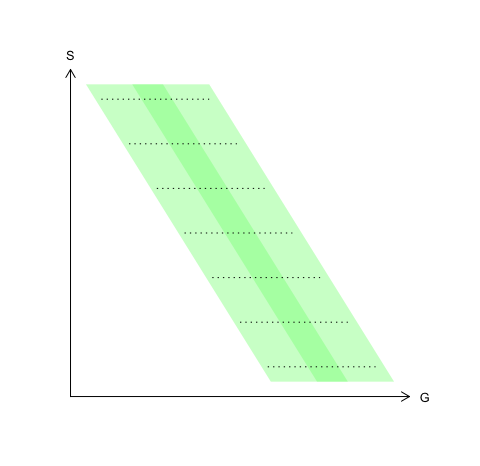
\includegraphics[width=0.5\columnwidth]{correlation-counterexample}
\par\end{centering}
\caption{Correlation counterexample\label{fig:Correlation-counterexample}}

\end{figure}

\hypertarget{proof-of-proposition}{%
\subsection{\texorpdfstring{Proof of Proposition \ref{prop:robustness}}{Proof of Proposition }}\label{proof-of-proposition}}

\begin{proof}

Note that in proposition \ref{prop:prop1}, we took $g_{c(i)} = \bar{g}_{i}$ and $s_{c(i)} = \bar{s}_i$. Write 
\begin{align}
cov(G_{c},S_{c}) & =cov(\bar{G}+\varepsilon^{G},\bar{S}+\varepsilon^{S})\nonumber \\
 & = cov(\bar{G},\bar{S}) + cov(\varepsilon^{G},\bar{S}) + 
     cov(\bar{G},\varepsilon^{S}) + cov(\varepsilon^{G},\varepsilon^{S}).
 \label{eq:cov-with-error}
\end{align}
For any $X$ and $Y$, $cov(X, Y)$ is bounded by $\sqrt{var(X) var(Y)}$.
Plugging $\sigma_{G}^{2}$ and $\sigma_{S}^{2}$ into this formula
shows that under condition 1, $cov(G_{c},S_{c})$ will be arbitrarily
close to $cov(\bar{G},\bar{S})$. Similarly, writing
\[
var(G_{c}) = var(\bar{G}) + var(\varepsilon^{G}) + 2cov(\bar{G},\varepsilon^{G})
\]
shows that $var(G_{c})$ will approach $var(\bar{G})$ as $\sigma_{G}^{2}$
grows small, and similarly for $var(S_{c})$. Plugging these facts
into (\ref{eq:corr-cov-var}) shows that $corr(G_{c},S_{c})$ approaches
$corr(\bar{G},\bar{S})$ as $\sigma_{G}^{2}$ and $\sigma_{S}^{2}$
grow small. Proposition 1 then shows $corr(\bar{G},\bar{S}) < corr(G_{p},S_{p})$
for $k\in(0,1)$.

Under condition 2, $cov(G_{c}, S_{c}) = cov(\bar{G},\bar{S})$ since
the last three terms of the sum in (\ref{eq:cov-with-error}) are
zero. Then since 
\[
cov(\bar{G},\bar{S})\ge cov(G_{p},S_{p}) = 0
\]
with strict inequality iff $k\in(0,1)$, the covariance signs the
correlation. 

\end{proof}

\FloatBarrier

\newpage

\hypertarget{robustness-checks}{%
\subsection{Robustness checks}\label{robustness-checks}}

Table \ref{tab:tbl-bo-psea-no-par-age} reruns our central regressions,
dropping the control for parents' age at birth. Results show the same
pattern as in the main text: the coefficient for birth order is
negative, but changes sign when university attendance is added as a
potential mediator. However, the birth order effect is smaller overall,
and is never significant. We also ran regressions using father's age
only; results are similar to those in the main text.

Table \ref{tab:tbl-bo-psea-dummies} reruns our central regressions but
includes a separate coefficient for each position in the birth order
(with firstborn as the baseline). The basic pattern of our main result
holds: birth order coefficients are generally negative; adding mediators
causes them to increase towards zero or to change sign. Birth order
effects appear largest for birth order 2-3. However, effects for later
birth orders are also imprecisely estimated (since fewer respondents
come from large families).

Notably when we add income, dummies for birth order 5 and 6 become large
and positive. This could be (for instance) because being the last born
has advantages after effects on SES have been netted out. Table
\ref{tab:tbl-bo-subset-dummies} runs the same exercise for different
subsets: male respondents, female respondents, and couples with
children. The basic pattern that birth order coefficients shrink after
adding mediators is quite robust. Note however that here, the estimates
of effects for birth order 2-3 are larger for females.

We also ran a specification with separate birth order dummies within
each family size. Figure \ref{fig:pic-bo-psea-interactions} shows 95\%
confidence intervals for the birth order coefficients, from the column 2
specification including height and IQ controls but no mediators. Not
surprisingly, coefficients are imprecisely estimated. But most birth
order coefficients are negative compared to the baseline for firstborns.

Table \ref{tab:tbl-bo-psea-pgs} reruns our regressions controlling for
several polygenic scores. Results are very close to those in the main
text.

Table \ref{tab:tbl-bo-psea-age-fte} reruns relevant columns of Table
\ref{tab:tbl-bo-psea} using age of leaving full-time education as a
measure of educational SES, instead of the university attendance dummy.
Results are similar to those in the main text: controlling for age of
leaving full-time education shrinks the effect of birth order and makes
it insignificant.

Table \ref{tab:tbl-bo-psea-no3} reruns Table \ref{tab:tbl-bo-psea}
excluding families of size 3. Results are very similar to those in the
main text.

Chiappori, Oreffice, and Quintana-Domeque (2012) write down a matching model in which a person's
attractiveness is summarized by a single index. The linear version of the
model can be tested by regressing one partner's characteristics on each of the
other partner's characteristics in turn (using Seemingly Unrelated
Regressions), and checking that the coefficients have the same proportions
across each regression. We do this for birth order and PSEA. Table
\ref{tab:tbl-sur} shows the results. We exclude year of birth dummies,
since they cause the estimation procedure to fail.

We also check the proportionality of coefficients. We run a Wald test that

\[
\frac{\beta^{PSEA}_{PSEA}}{\beta^{PSEA}_{BO}} =
\frac{\beta^{BO}_{PSEA}}{\beta^{BO}_{BO}}
\]

where e.g.~\(\beta^{PSEA}_{BO}\) is the coefficient of birth order in the
regression targeting PSEA. P values are \(p\) =
0.24 for males and \(p\) =
0.022 for females. So for females there
is some evidence against this linear model.

 
  \providecommand{\huxb}[2]{\arrayrulecolor[RGB]{#1}\global\arrayrulewidth=#2pt}
  \providecommand{\huxvb}[2]{\color[RGB]{#1}\vrule width #2pt}
  \providecommand{\huxtpad}[1]{\rule{0pt}{#1}}
  \providecommand{\huxbpad}[1]{\rule[-#1]{0pt}{#1}}

\begin{table}[ht]
\begin{centerbox}
\begin{threeparttable}
\captionsetup{justification=centering,singlelinecheck=off}
\caption{\label{tab:tbl-bo-psea-no-par-age} Regressions of spouse PSEA, without controls for parents' age at respondent's birth}
 \setlength{\tabcolsep}{0pt}
\begin{tabular}{l l l l l}


\hhline{>{\huxb{0, 0, 0}{0.8}}->{\huxb{0, 0, 0}{0.8}}->{\huxb{0, 0, 0}{0.8}}->{\huxb{0, 0, 0}{0.8}}->{\huxb{0, 0, 0}{0.8}}-}
\arrayrulecolor{black}

\multicolumn{1}{!{\huxvb{0, 0, 0}{0}}c!{\huxvb{0, 0, 0}{0}}}{\huxtpad{6pt + 1em}\centering \hspace{6pt}  \hspace{6pt}\huxbpad{6pt}} &
\multicolumn{1}{c!{\huxvb{0, 0, 0}{0}}}{\huxtpad{6pt + 1em}\centering \hspace{6pt} (1) \hspace{6pt}\huxbpad{6pt}} &
\multicolumn{1}{c!{\huxvb{0, 0, 0}{0}}}{\huxtpad{6pt + 1em}\centering \hspace{6pt} (2) \hspace{6pt}\huxbpad{6pt}} &
\multicolumn{1}{c!{\huxvb{0, 0, 0}{0}}}{\huxtpad{6pt + 1em}\centering \hspace{6pt} (3) \hspace{6pt}\huxbpad{6pt}} &
\multicolumn{1}{c!{\huxvb{0, 0, 0}{0}}}{\huxtpad{6pt + 1em}\centering \hspace{6pt} (4) \hspace{6pt}\huxbpad{6pt}} \tabularnewline[-0.5pt]


\hhline{>{\huxb{255, 255, 255}{0.4}}->{\huxb{0, 0, 0}{0.4}}->{\huxb{0, 0, 0}{0.4}}->{\huxb{0, 0, 0}{0.4}}->{\huxb{0, 0, 0}{0.4}}-}
\arrayrulecolor{black}

\multicolumn{1}{!{\huxvb{0, 0, 0}{0}}l!{\huxvb{0, 0, 0}{0}}}{\huxtpad{6pt + 1em}\raggedright \hspace{6pt} Birth order \hspace{6pt}\huxbpad{6pt}} &
\multicolumn{1}{r!{\huxvb{0, 0, 0}{0}}}{\huxtpad{6pt + 1em}\raggedleft \hspace{6pt} $-$0.0079~~~~ \hspace{6pt}\huxbpad{6pt}} &
\multicolumn{1}{r!{\huxvb{0, 0, 0}{0}}}{\huxtpad{6pt + 1em}\raggedleft \hspace{6pt} 0.0026~~~~ \hspace{6pt}\huxbpad{6pt}} &
\multicolumn{1}{r!{\huxvb{0, 0, 0}{0}}}{\huxtpad{6pt + 1em}\raggedleft \hspace{6pt} $-$0.0030~~~~ \hspace{6pt}\huxbpad{6pt}} &
\multicolumn{1}{r!{\huxvb{0, 0, 0}{0}}}{\huxtpad{6pt + 1em}\raggedleft \hspace{6pt} 0.0018~~~~ \hspace{6pt}\huxbpad{6pt}} \tabularnewline[-0.5pt]


\hhline{}
\arrayrulecolor{black}

\multicolumn{1}{!{\huxvb{0, 0, 0}{0}}l!{\huxvb{0, 0, 0}{0}}}{\huxtpad{6pt + 1em}\raggedright \hspace{6pt}  \hspace{6pt}\huxbpad{6pt}} &
\multicolumn{1}{r!{\huxvb{0, 0, 0}{0}}}{\huxtpad{6pt + 1em}\raggedleft \hspace{6pt} (0.0074)~~~ \hspace{6pt}\huxbpad{6pt}} &
\multicolumn{1}{r!{\huxvb{0, 0, 0}{0}}}{\huxtpad{6pt + 1em}\raggedleft \hspace{6pt} (0.0074)~~~ \hspace{6pt}\huxbpad{6pt}} &
\multicolumn{1}{r!{\huxvb{0, 0, 0}{0}}}{\huxtpad{6pt + 1em}\raggedleft \hspace{6pt} (0.0137)~~~ \hspace{6pt}\huxbpad{6pt}} &
\multicolumn{1}{r!{\huxvb{0, 0, 0}{0}}}{\huxtpad{6pt + 1em}\raggedleft \hspace{6pt} (0.0137)~~~ \hspace{6pt}\huxbpad{6pt}} \tabularnewline[-0.5pt]


\hhline{}
\arrayrulecolor{black}

\multicolumn{1}{!{\huxvb{0, 0, 0}{0}}l!{\huxvb{0, 0, 0}{0}}}{\huxtpad{6pt + 1em}\raggedright \hspace{6pt} University \hspace{6pt}\huxbpad{6pt}} &
\multicolumn{1}{r!{\huxvb{0, 0, 0}{0}}}{\huxtpad{6pt + 1em}\raggedleft \hspace{6pt} ~~~~~~~~~ \hspace{6pt}\huxbpad{6pt}} &
\multicolumn{1}{r!{\huxvb{0, 0, 0}{0}}}{\huxtpad{6pt + 1em}\raggedleft \hspace{6pt} 0.2504 *** \hspace{6pt}\huxbpad{6pt}} &
\multicolumn{1}{r!{\huxvb{0, 0, 0}{0}}}{\huxtpad{6pt + 1em}\raggedleft \hspace{6pt} ~~~~~~~~~ \hspace{6pt}\huxbpad{6pt}} &
\multicolumn{1}{r!{\huxvb{0, 0, 0}{0}}}{\huxtpad{6pt + 1em}\raggedleft \hspace{6pt} 0.2064 *** \hspace{6pt}\huxbpad{6pt}} \tabularnewline[-0.5pt]


\hhline{}
\arrayrulecolor{black}

\multicolumn{1}{!{\huxvb{0, 0, 0}{0}}l!{\huxvb{0, 0, 0}{0}}}{\huxtpad{6pt + 1em}\raggedright \hspace{6pt}  \hspace{6pt}\huxbpad{6pt}} &
\multicolumn{1}{r!{\huxvb{0, 0, 0}{0}}}{\huxtpad{6pt + 1em}\raggedleft \hspace{6pt} ~~~~~~~~~ \hspace{6pt}\huxbpad{6pt}} &
\multicolumn{1}{r!{\huxvb{0, 0, 0}{0}}}{\huxtpad{6pt + 1em}\raggedleft \hspace{6pt} (0.0148)~~~ \hspace{6pt}\huxbpad{6pt}} &
\multicolumn{1}{r!{\huxvb{0, 0, 0}{0}}}{\huxtpad{6pt + 1em}\raggedleft \hspace{6pt} ~~~~~~~~~ \hspace{6pt}\huxbpad{6pt}} &
\multicolumn{1}{r!{\huxvb{0, 0, 0}{0}}}{\huxtpad{6pt + 1em}\raggedleft \hspace{6pt} (0.0250)~~~ \hspace{6pt}\huxbpad{6pt}} \tabularnewline[-0.5pt]


\hhline{}
\arrayrulecolor{black}

\multicolumn{1}{!{\huxvb{0, 0, 0}{0}}l!{\huxvb{0, 0, 0}{0}}}{\huxtpad{6pt + 1em}\raggedright \hspace{6pt} Income \hspace{6pt}\huxbpad{6pt}} &
\multicolumn{1}{r!{\huxvb{0, 0, 0}{0}}}{\huxtpad{6pt + 1em}\raggedleft \hspace{6pt} ~~~~~~~~~ \hspace{6pt}\huxbpad{6pt}} &
\multicolumn{1}{r!{\huxvb{0, 0, 0}{0}}}{\huxtpad{6pt + 1em}\raggedleft \hspace{6pt} ~~~~~~~~~ \hspace{6pt}\huxbpad{6pt}} &
\multicolumn{1}{r!{\huxvb{0, 0, 0}{0}}}{\huxtpad{6pt + 1em}\raggedleft \hspace{6pt} 0.0033 *** \hspace{6pt}\huxbpad{6pt}} &
\multicolumn{1}{r!{\huxvb{0, 0, 0}{0}}}{\huxtpad{6pt + 1em}\raggedleft \hspace{6pt} 0.0022 **~ \hspace{6pt}\huxbpad{6pt}} \tabularnewline[-0.5pt]


\hhline{}
\arrayrulecolor{black}

\multicolumn{1}{!{\huxvb{0, 0, 0}{0}}l!{\huxvb{0, 0, 0}{0}}}{\huxtpad{6pt + 1em}\raggedright \hspace{6pt}  \hspace{6pt}\huxbpad{6pt}} &
\multicolumn{1}{r!{\huxvb{0, 0, 0}{0}}}{\huxtpad{6pt + 1em}\raggedleft \hspace{6pt} ~~~~~~~~~ \hspace{6pt}\huxbpad{6pt}} &
\multicolumn{1}{r!{\huxvb{0, 0, 0}{0}}}{\huxtpad{6pt + 1em}\raggedleft \hspace{6pt} ~~~~~~~~~ \hspace{6pt}\huxbpad{6pt}} &
\multicolumn{1}{r!{\huxvb{0, 0, 0}{0}}}{\huxtpad{6pt + 1em}\raggedleft \hspace{6pt} (0.0008)~~~ \hspace{6pt}\huxbpad{6pt}} &
\multicolumn{1}{r!{\huxvb{0, 0, 0}{0}}}{\huxtpad{6pt + 1em}\raggedleft \hspace{6pt} (0.0008)~~~ \hspace{6pt}\huxbpad{6pt}} \tabularnewline[-0.5pt]


\hhline{}
\arrayrulecolor{black}

\multicolumn{1}{!{\huxvb{0, 0, 0}{0}}l!{\huxvb{0, 0, 0}{0}}}{\huxtpad{6pt + 1em}\raggedright \hspace{6pt} Own PSEA \hspace{6pt}\huxbpad{6pt}} &
\multicolumn{1}{r!{\huxvb{0, 0, 0}{0}}}{\huxtpad{6pt + 1em}\raggedleft \hspace{6pt} 0.0651 *** \hspace{6pt}\huxbpad{6pt}} &
\multicolumn{1}{r!{\huxvb{0, 0, 0}{0}}}{\huxtpad{6pt + 1em}\raggedleft \hspace{6pt} 0.0366 *** \hspace{6pt}\huxbpad{6pt}} &
\multicolumn{1}{r!{\huxvb{0, 0, 0}{0}}}{\huxtpad{6pt + 1em}\raggedleft \hspace{6pt} 0.0471 *** \hspace{6pt}\huxbpad{6pt}} &
\multicolumn{1}{r!{\huxvb{0, 0, 0}{0}}}{\huxtpad{6pt + 1em}\raggedleft \hspace{6pt} 0.0335 **~ \hspace{6pt}\huxbpad{6pt}} \tabularnewline[-0.5pt]


\hhline{}
\arrayrulecolor{black}

\multicolumn{1}{!{\huxvb{0, 0, 0}{0}}l!{\huxvb{0, 0, 0}{0}}}{\huxtpad{6pt + 1em}\raggedright \hspace{6pt}  \hspace{6pt}\huxbpad{6pt}} &
\multicolumn{1}{r!{\huxvb{0, 0, 0}{0}}}{\huxtpad{6pt + 1em}\raggedleft \hspace{6pt} (0.0065)~~~ \hspace{6pt}\huxbpad{6pt}} &
\multicolumn{1}{r!{\huxvb{0, 0, 0}{0}}}{\huxtpad{6pt + 1em}\raggedleft \hspace{6pt} (0.0066)~~~ \hspace{6pt}\huxbpad{6pt}} &
\multicolumn{1}{r!{\huxvb{0, 0, 0}{0}}}{\huxtpad{6pt + 1em}\raggedleft \hspace{6pt} (0.0120)~~~ \hspace{6pt}\huxbpad{6pt}} &
\multicolumn{1}{r!{\huxvb{0, 0, 0}{0}}}{\huxtpad{6pt + 1em}\raggedleft \hspace{6pt} (0.0120)~~~ \hspace{6pt}\huxbpad{6pt}} \tabularnewline[-0.5pt]


\hhline{}
\arrayrulecolor{black}

\multicolumn{1}{!{\huxvb{0, 0, 0}{0}}l!{\huxvb{0, 0, 0}{0}}}{\huxtpad{6pt + 1em}\raggedright \hspace{6pt} Fluid IQ \hspace{6pt}\huxbpad{6pt}} &
\multicolumn{1}{r!{\huxvb{0, 0, 0}{0}}}{\huxtpad{6pt + 1em}\raggedleft \hspace{6pt} ~~~~~~~~~ \hspace{6pt}\huxbpad{6pt}} &
\multicolumn{1}{r!{\huxvb{0, 0, 0}{0}}}{\huxtpad{6pt + 1em}\raggedleft \hspace{6pt} 0.0165 *** \hspace{6pt}\huxbpad{6pt}} &
\multicolumn{1}{r!{\huxvb{0, 0, 0}{0}}}{\huxtpad{6pt + 1em}\raggedleft \hspace{6pt} 0.0173 **~ \hspace{6pt}\huxbpad{6pt}} &
\multicolumn{1}{r!{\huxvb{0, 0, 0}{0}}}{\huxtpad{6pt + 1em}\raggedleft \hspace{6pt} 0.0051~~~~ \hspace{6pt}\huxbpad{6pt}} \tabularnewline[-0.5pt]


\hhline{}
\arrayrulecolor{black}

\multicolumn{1}{!{\huxvb{0, 0, 0}{0}}l!{\huxvb{0, 0, 0}{0}}}{\huxtpad{6pt + 1em}\raggedright \hspace{6pt}  \hspace{6pt}\huxbpad{6pt}} &
\multicolumn{1}{r!{\huxvb{0, 0, 0}{0}}}{\huxtpad{6pt + 1em}\raggedleft \hspace{6pt} ~~~~~~~~~ \hspace{6pt}\huxbpad{6pt}} &
\multicolumn{1}{r!{\huxvb{0, 0, 0}{0}}}{\huxtpad{6pt + 1em}\raggedleft \hspace{6pt} (0.0034)~~~ \hspace{6pt}\huxbpad{6pt}} &
\multicolumn{1}{r!{\huxvb{0, 0, 0}{0}}}{\huxtpad{6pt + 1em}\raggedleft \hspace{6pt} (0.0060)~~~ \hspace{6pt}\huxbpad{6pt}} &
\multicolumn{1}{r!{\huxvb{0, 0, 0}{0}}}{\huxtpad{6pt + 1em}\raggedleft \hspace{6pt} (0.0062)~~~ \hspace{6pt}\huxbpad{6pt}} \tabularnewline[-0.5pt]


\hhline{}
\arrayrulecolor{black}

\multicolumn{1}{!{\huxvb{0, 0, 0}{0}}l!{\huxvb{0, 0, 0}{0}}}{\huxtpad{6pt + 1em}\raggedright \hspace{6pt} Height \hspace{6pt}\huxbpad{6pt}} &
\multicolumn{1}{r!{\huxvb{0, 0, 0}{0}}}{\huxtpad{6pt + 1em}\raggedleft \hspace{6pt} ~~~~~~~~~ \hspace{6pt}\huxbpad{6pt}} &
\multicolumn{1}{r!{\huxvb{0, 0, 0}{0}}}{\huxtpad{6pt + 1em}\raggedleft \hspace{6pt} 0.0019 **~ \hspace{6pt}\huxbpad{6pt}} &
\multicolumn{1}{r!{\huxvb{0, 0, 0}{0}}}{\huxtpad{6pt + 1em}\raggedleft \hspace{6pt} 0.0037 **~ \hspace{6pt}\huxbpad{6pt}} &
\multicolumn{1}{r!{\huxvb{0, 0, 0}{0}}}{\huxtpad{6pt + 1em}\raggedleft \hspace{6pt} 0.0032 *~~ \hspace{6pt}\huxbpad{6pt}} \tabularnewline[-0.5pt]


\hhline{}
\arrayrulecolor{black}

\multicolumn{1}{!{\huxvb{0, 0, 0}{0}}l!{\huxvb{0, 0, 0}{0}}}{\huxtpad{6pt + 1em}\raggedright \hspace{6pt}  \hspace{6pt}\huxbpad{6pt}} &
\multicolumn{1}{r!{\huxvb{0, 0, 0}{0}}}{\huxtpad{6pt + 1em}\raggedleft \hspace{6pt} ~~~~~~~~~ \hspace{6pt}\huxbpad{6pt}} &
\multicolumn{1}{r!{\huxvb{0, 0, 0}{0}}}{\huxtpad{6pt + 1em}\raggedleft \hspace{6pt} (0.0007)~~~ \hspace{6pt}\huxbpad{6pt}} &
\multicolumn{1}{r!{\huxvb{0, 0, 0}{0}}}{\huxtpad{6pt + 1em}\raggedleft \hspace{6pt} (0.0013)~~~ \hspace{6pt}\huxbpad{6pt}} &
\multicolumn{1}{r!{\huxvb{0, 0, 0}{0}}}{\huxtpad{6pt + 1em}\raggedleft \hspace{6pt} (0.0013)~~~ \hspace{6pt}\huxbpad{6pt}} \tabularnewline[-0.5pt]


\hhline{>{\huxb{255, 255, 255}{0.4}}->{\huxb{0, 0, 0}{0.4}}->{\huxb{0, 0, 0}{0.4}}->{\huxb{0, 0, 0}{0.4}}->{\huxb{0, 0, 0}{0.4}}-}
\arrayrulecolor{black}

\multicolumn{1}{!{\huxvb{0, 0, 0}{0}}l!{\huxvb{0, 0, 0}{0}}}{\huxtpad{6pt + 1em}\raggedright \hspace{6pt} Family size dummies \hspace{6pt}\huxbpad{6pt}} &
\multicolumn{1}{c!{\huxvb{0, 0, 0}{0}}}{\huxtpad{6pt + 1em}\centering \hspace{6pt} Yes \hspace{6pt}\huxbpad{6pt}} &
\multicolumn{1}{c!{\huxvb{0, 0, 0}{0}}}{\huxtpad{6pt + 1em}\centering \hspace{6pt} Yes \hspace{6pt}\huxbpad{6pt}} &
\multicolumn{1}{c!{\huxvb{0, 0, 0}{0}}}{\huxtpad{6pt + 1em}\centering \hspace{6pt} Yes \hspace{6pt}\huxbpad{6pt}} &
\multicolumn{1}{c!{\huxvb{0, 0, 0}{0}}}{\huxtpad{6pt + 1em}\centering \hspace{6pt} Yes \hspace{6pt}\huxbpad{6pt}} \tabularnewline[-0.5pt]


\hhline{}
\arrayrulecolor{black}

\multicolumn{1}{!{\huxvb{0, 0, 0}{0}}l!{\huxvb{0, 0, 0}{0}}}{\huxtpad{6pt + 1em}\raggedright \hspace{6pt} Birth month dummies \hspace{6pt}\huxbpad{6pt}} &
\multicolumn{1}{c!{\huxvb{0, 0, 0}{0}}}{\huxtpad{6pt + 1em}\centering \hspace{6pt} Yes \hspace{6pt}\huxbpad{6pt}} &
\multicolumn{1}{c!{\huxvb{0, 0, 0}{0}}}{\huxtpad{6pt + 1em}\centering \hspace{6pt} Yes \hspace{6pt}\huxbpad{6pt}} &
\multicolumn{1}{c!{\huxvb{0, 0, 0}{0}}}{\huxtpad{6pt + 1em}\centering \hspace{6pt} Yes \hspace{6pt}\huxbpad{6pt}} &
\multicolumn{1}{c!{\huxvb{0, 0, 0}{0}}}{\huxtpad{6pt + 1em}\centering \hspace{6pt} Yes \hspace{6pt}\huxbpad{6pt}} \tabularnewline[-0.5pt]


\hhline{}
\arrayrulecolor{black}

\multicolumn{1}{!{\huxvb{0, 0, 0}{0}}l!{\huxvb{0, 0, 0}{0}}}{\huxtpad{6pt + 1em}\raggedright \hspace{6pt} Birth year dummies \hspace{6pt}\huxbpad{6pt}} &
\multicolumn{1}{c!{\huxvb{0, 0, 0}{0}}}{\huxtpad{6pt + 1em}\centering \hspace{6pt} Yes \hspace{6pt}\huxbpad{6pt}} &
\multicolumn{1}{c!{\huxvb{0, 0, 0}{0}}}{\huxtpad{6pt + 1em}\centering \hspace{6pt} Yes \hspace{6pt}\huxbpad{6pt}} &
\multicolumn{1}{c!{\huxvb{0, 0, 0}{0}}}{\huxtpad{6pt + 1em}\centering \hspace{6pt} Yes \hspace{6pt}\huxbpad{6pt}} &
\multicolumn{1}{c!{\huxvb{0, 0, 0}{0}}}{\huxtpad{6pt + 1em}\centering \hspace{6pt} Yes \hspace{6pt}\huxbpad{6pt}} \tabularnewline[-0.5pt]


\hhline{>{\huxb{255, 255, 255}{0.4}}->{\huxb{0, 0, 0}{0.4}}->{\huxb{0, 0, 0}{0.4}}->{\huxb{0, 0, 0}{0.4}}->{\huxb{0, 0, 0}{0.4}}-}
\arrayrulecolor{black}

\multicolumn{1}{!{\huxvb{0, 0, 0}{0}}l!{\huxvb{0, 0, 0}{0}}}{\huxtpad{6pt + 1em}\raggedright \hspace{6pt} N \hspace{6pt}\huxbpad{6pt}} &
\multicolumn{1}{r!{\huxvb{0, 0, 0}{0}}}{\huxtpad{6pt + 1em}\raggedleft \hspace{6pt} 23861~~~~~~~~~ \hspace{6pt}\huxbpad{6pt}} &
\multicolumn{1}{r!{\huxvb{0, 0, 0}{0}}}{\huxtpad{6pt + 1em}\raggedleft \hspace{6pt} 23861~~~~~~~~~ \hspace{6pt}\huxbpad{6pt}} &
\multicolumn{1}{r!{\huxvb{0, 0, 0}{0}}}{\huxtpad{6pt + 1em}\raggedleft \hspace{6pt} 7673~~~~~~~~~ \hspace{6pt}\huxbpad{6pt}} &
\multicolumn{1}{r!{\huxvb{0, 0, 0}{0}}}{\huxtpad{6pt + 1em}\raggedleft \hspace{6pt} 7673~~~~~~~~~ \hspace{6pt}\huxbpad{6pt}} \tabularnewline[-0.5pt]


\hhline{}
\arrayrulecolor{black}

\multicolumn{1}{!{\huxvb{0, 0, 0}{0}}l!{\huxvb{0, 0, 0}{0}}}{\huxtpad{6pt + 1em}\raggedright \hspace{6pt} R2 \hspace{6pt}\huxbpad{6pt}} &
\multicolumn{1}{r!{\huxvb{0, 0, 0}{0}}}{\huxtpad{6pt + 1em}\raggedleft \hspace{6pt} 0.011~~~~~ \hspace{6pt}\huxbpad{6pt}} &
\multicolumn{1}{r!{\huxvb{0, 0, 0}{0}}}{\huxtpad{6pt + 1em}\raggedleft \hspace{6pt} 0.028~~~~~ \hspace{6pt}\huxbpad{6pt}} &
\multicolumn{1}{r!{\huxvb{0, 0, 0}{0}}}{\huxtpad{6pt + 1em}\raggedleft \hspace{6pt} 0.018~~~~~ \hspace{6pt}\huxbpad{6pt}} &
\multicolumn{1}{r!{\huxvb{0, 0, 0}{0}}}{\huxtpad{6pt + 1em}\raggedleft \hspace{6pt} 0.027~~~~~ \hspace{6pt}\huxbpad{6pt}} \tabularnewline[-0.5pt]


\hhline{}
\arrayrulecolor{black}

\multicolumn{1}{!{\huxvb{0, 0, 0}{0}}l!{\huxvb{0, 0, 0}{0}}}{\huxtpad{6pt + 1em}\raggedright \hspace{6pt} logLik \hspace{6pt}\huxbpad{6pt}} &
\multicolumn{1}{r!{\huxvb{0, 0, 0}{0}}}{\huxtpad{6pt + 1em}\raggedleft \hspace{6pt} $-$33521.263~~~~~ \hspace{6pt}\huxbpad{6pt}} &
\multicolumn{1}{r!{\huxvb{0, 0, 0}{0}}}{\huxtpad{6pt + 1em}\raggedleft \hspace{6pt} $-$33311.976~~~~~ \hspace{6pt}\huxbpad{6pt}} &
\multicolumn{1}{r!{\huxvb{0, 0, 0}{0}}}{\huxtpad{6pt + 1em}\raggedleft \hspace{6pt} $-$10771.954~~~~~ \hspace{6pt}\huxbpad{6pt}} &
\multicolumn{1}{r!{\huxvb{0, 0, 0}{0}}}{\huxtpad{6pt + 1em}\raggedleft \hspace{6pt} $-$10737.107~~~~~ \hspace{6pt}\huxbpad{6pt}} \tabularnewline[-0.5pt]


\hhline{}
\arrayrulecolor{black}

\multicolumn{1}{!{\huxvb{0, 0, 0}{0}}l!{\huxvb{0, 0, 0}{0}}}{\huxtpad{6pt + 1em}\raggedright \hspace{6pt} AIC \hspace{6pt}\huxbpad{6pt}} &
\multicolumn{1}{r!{\huxvb{0, 0, 0}{0}}}{\huxtpad{6pt + 1em}\raggedleft \hspace{6pt} 67144.525~~~~~ \hspace{6pt}\huxbpad{6pt}} &
\multicolumn{1}{r!{\huxvb{0, 0, 0}{0}}}{\huxtpad{6pt + 1em}\raggedleft \hspace{6pt} 66731.953~~~~~ \hspace{6pt}\huxbpad{6pt}} &
\multicolumn{1}{r!{\huxvb{0, 0, 0}{0}}}{\huxtpad{6pt + 1em}\raggedleft \hspace{6pt} 21649.909~~~~~ \hspace{6pt}\huxbpad{6pt}} &
\multicolumn{1}{r!{\huxvb{0, 0, 0}{0}}}{\huxtpad{6pt + 1em}\raggedleft \hspace{6pt} 21582.215~~~~~ \hspace{6pt}\huxbpad{6pt}} \tabularnewline[-0.5pt]


\hhline{>{\huxb{0, 0, 0}{0.8}}->{\huxb{0, 0, 0}{0.8}}->{\huxb{0, 0, 0}{0.8}}->{\huxb{0, 0, 0}{0.8}}->{\huxb{0, 0, 0}{0.8}}-}
\arrayrulecolor{black}

\multicolumn{5}{!{\huxvb{0, 0, 0}{0}}l!{\huxvb{0, 0, 0}{0}}}{\huxtpad{6pt + 1em}\raggedright \hspace{6pt}  *** p $<$ 0.001;  ** p $<$ 0.01;  * p $<$ 0.05;  + p $<$ 0.1. Standard errors: robust. \hspace{6pt}\huxbpad{6pt}} \tabularnewline[-0.5pt]


\hhline{}
\arrayrulecolor{black}
\end{tabular}
\end{threeparttable}\par\end{centerbox}

\end{table}
 

 
  \providecommand{\huxb}[2]{\arrayrulecolor[RGB]{#1}\global\arrayrulewidth=#2pt}
  \providecommand{\huxvb}[2]{\color[RGB]{#1}\vrule width #2pt}
  \providecommand{\huxtpad}[1]{\rule{0pt}{#1}}
  \providecommand{\huxbpad}[1]{\rule[-#1]{0pt}{#1}}

\begin{table}[ht]
\begin{centerbox}
\begin{threeparttable}
\captionsetup{justification=centering,singlelinecheck=off}
\caption{\label{tab:tbl-bo-psea-dummies} Regressions of spouse PSEA, separate birth order dummies}
 \setlength{\tabcolsep}{0pt}
\begin{tabular}{l l l l l}


\hhline{>{\huxb{0, 0, 0}{0.8}}->{\huxb{0, 0, 0}{0.8}}->{\huxb{0, 0, 0}{0.8}}->{\huxb{0, 0, 0}{0.8}}->{\huxb{0, 0, 0}{0.8}}-}
\arrayrulecolor{black}

\multicolumn{1}{!{\huxvb{0, 0, 0}{0}}c!{\huxvb{0, 0, 0}{0}}}{\huxtpad{3pt + 1em}\centering \hspace{6pt} {\fontsize{10pt}{12pt}\selectfont } \hspace{6pt}\huxbpad{3pt}} &
\multicolumn{1}{c!{\huxvb{0, 0, 0}{0}}}{\huxtpad{3pt + 1em}\centering \hspace{6pt} {\fontsize{10pt}{12pt}\selectfont (1)} \hspace{6pt}\huxbpad{3pt}} &
\multicolumn{1}{c!{\huxvb{0, 0, 0}{0}}}{\huxtpad{3pt + 1em}\centering \hspace{6pt} {\fontsize{10pt}{12pt}\selectfont (2)} \hspace{6pt}\huxbpad{3pt}} &
\multicolumn{1}{c!{\huxvb{0, 0, 0}{0}}}{\huxtpad{3pt + 1em}\centering \hspace{6pt} {\fontsize{10pt}{12pt}\selectfont (3)} \hspace{6pt}\huxbpad{3pt}} &
\multicolumn{1}{c!{\huxvb{0, 0, 0}{0}}}{\huxtpad{3pt + 1em}\centering \hspace{6pt} {\fontsize{10pt}{12pt}\selectfont (4)} \hspace{6pt}\huxbpad{3pt}} \tabularnewline[-0.5pt]


\hhline{>{\huxb{255, 255, 255}{0.4}}->{\huxb{0, 0, 0}{0.4}}->{\huxb{0, 0, 0}{0.4}}->{\huxb{0, 0, 0}{0.4}}->{\huxb{0, 0, 0}{0.4}}-}
\arrayrulecolor{black}

\multicolumn{1}{!{\huxvb{0, 0, 0}{0}}l!{\huxvb{0, 0, 0}{0}}}{\huxtpad{3pt + 1em}\raggedright \hspace{6pt} {\fontsize{10pt}{12pt}\selectfont Birth order 2} \hspace{6pt}\huxbpad{3pt}} &
\multicolumn{1}{r!{\huxvb{0, 0, 0}{0}}}{\huxtpad{3pt + 1em}\raggedleft \hspace{6pt} {\fontsize{10pt}{12pt}\selectfont $-$0.0492 *~~} \hspace{6pt}\huxbpad{3pt}} &
\multicolumn{1}{r!{\huxvb{0, 0, 0}{0}}}{\huxtpad{3pt + 1em}\raggedleft \hspace{6pt} {\fontsize{10pt}{12pt}\selectfont $-$0.0204~~~~} \hspace{6pt}\huxbpad{3pt}} &
\multicolumn{1}{r!{\huxvb{0, 0, 0}{0}}}{\huxtpad{3pt + 1em}\raggedleft \hspace{6pt} {\fontsize{10pt}{12pt}\selectfont $-$0.0466~~~~} \hspace{6pt}\huxbpad{3pt}} &
\multicolumn{1}{r!{\huxvb{0, 0, 0}{0}}}{\huxtpad{3pt + 1em}\raggedleft \hspace{6pt} {\fontsize{10pt}{12pt}\selectfont $-$0.0445~~~~} \hspace{6pt}\huxbpad{3pt}} \tabularnewline[-0.5pt]


\hhline{}
\arrayrulecolor{black}

\multicolumn{1}{!{\huxvb{0, 0, 0}{0}}l!{\huxvb{0, 0, 0}{0}}}{\huxtpad{3pt + 1em}\raggedright \hspace{6pt} {\fontsize{10pt}{12pt}\selectfont } \hspace{6pt}\huxbpad{3pt}} &
\multicolumn{1}{r!{\huxvb{0, 0, 0}{0}}}{\huxtpad{3pt + 1em}\raggedleft \hspace{6pt} {\fontsize{10pt}{12pt}\selectfont (0.0232)~~~} \hspace{6pt}\huxbpad{3pt}} &
\multicolumn{1}{r!{\huxvb{0, 0, 0}{0}}}{\huxtpad{3pt + 1em}\raggedleft \hspace{6pt} {\fontsize{10pt}{12pt}\selectfont (0.0231)~~~} \hspace{6pt}\huxbpad{3pt}} &
\multicolumn{1}{r!{\huxvb{0, 0, 0}{0}}}{\huxtpad{3pt + 1em}\raggedleft \hspace{6pt} {\fontsize{10pt}{12pt}\selectfont (0.0411)~~~} \hspace{6pt}\huxbpad{3pt}} &
\multicolumn{1}{r!{\huxvb{0, 0, 0}{0}}}{\huxtpad{3pt + 1em}\raggedleft \hspace{6pt} {\fontsize{10pt}{12pt}\selectfont (0.0410)~~~} \hspace{6pt}\huxbpad{3pt}} \tabularnewline[-0.5pt]


\hhline{}
\arrayrulecolor{black}

\multicolumn{1}{!{\huxvb{0, 0, 0}{0}}l!{\huxvb{0, 0, 0}{0}}}{\huxtpad{3pt + 1em}\raggedright \hspace{6pt} {\fontsize{10pt}{12pt}\selectfont Birth order 3} \hspace{6pt}\huxbpad{3pt}} &
\multicolumn{1}{r!{\huxvb{0, 0, 0}{0}}}{\huxtpad{3pt + 1em}\raggedleft \hspace{6pt} {\fontsize{10pt}{12pt}\selectfont $-$0.0560~~~~} \hspace{6pt}\huxbpad{3pt}} &
\multicolumn{1}{r!{\huxvb{0, 0, 0}{0}}}{\huxtpad{3pt + 1em}\raggedleft \hspace{6pt} {\fontsize{10pt}{12pt}\selectfont $-$0.0049~~~~} \hspace{6pt}\huxbpad{3pt}} &
\multicolumn{1}{r!{\huxvb{0, 0, 0}{0}}}{\huxtpad{3pt + 1em}\raggedleft \hspace{6pt} {\fontsize{10pt}{12pt}\selectfont $-$0.0275~~~~} \hspace{6pt}\huxbpad{3pt}} &
\multicolumn{1}{r!{\huxvb{0, 0, 0}{0}}}{\huxtpad{3pt + 1em}\raggedleft \hspace{6pt} {\fontsize{10pt}{12pt}\selectfont $-$0.0066~~~~} \hspace{6pt}\huxbpad{3pt}} \tabularnewline[-0.5pt]


\hhline{}
\arrayrulecolor{black}

\multicolumn{1}{!{\huxvb{0, 0, 0}{0}}l!{\huxvb{0, 0, 0}{0}}}{\huxtpad{3pt + 1em}\raggedright \hspace{6pt} {\fontsize{10pt}{12pt}\selectfont } \hspace{6pt}\huxbpad{3pt}} &
\multicolumn{1}{r!{\huxvb{0, 0, 0}{0}}}{\huxtpad{3pt + 1em}\raggedleft \hspace{6pt} {\fontsize{10pt}{12pt}\selectfont (0.0375)~~~} \hspace{6pt}\huxbpad{3pt}} &
\multicolumn{1}{r!{\huxvb{0, 0, 0}{0}}}{\huxtpad{3pt + 1em}\raggedleft \hspace{6pt} {\fontsize{10pt}{12pt}\selectfont (0.0374)~~~} \hspace{6pt}\huxbpad{3pt}} &
\multicolumn{1}{r!{\huxvb{0, 0, 0}{0}}}{\huxtpad{3pt + 1em}\raggedleft \hspace{6pt} {\fontsize{10pt}{12pt}\selectfont (0.0672)~~~} \hspace{6pt}\huxbpad{3pt}} &
\multicolumn{1}{r!{\huxvb{0, 0, 0}{0}}}{\huxtpad{3pt + 1em}\raggedleft \hspace{6pt} {\fontsize{10pt}{12pt}\selectfont (0.0672)~~~} \hspace{6pt}\huxbpad{3pt}} \tabularnewline[-0.5pt]


\hhline{}
\arrayrulecolor{black}

\multicolumn{1}{!{\huxvb{0, 0, 0}{0}}l!{\huxvb{0, 0, 0}{0}}}{\huxtpad{3pt + 1em}\raggedright \hspace{6pt} {\fontsize{10pt}{12pt}\selectfont Birth order 4} \hspace{6pt}\huxbpad{3pt}} &
\multicolumn{1}{r!{\huxvb{0, 0, 0}{0}}}{\huxtpad{3pt + 1em}\raggedleft \hspace{6pt} {\fontsize{10pt}{12pt}\selectfont $-$0.0739~~~~} \hspace{6pt}\huxbpad{3pt}} &
\multicolumn{1}{r!{\huxvb{0, 0, 0}{0}}}{\huxtpad{3pt + 1em}\raggedleft \hspace{6pt} {\fontsize{10pt}{12pt}\selectfont $-$0.0006~~~~} \hspace{6pt}\huxbpad{3pt}} &
\multicolumn{1}{r!{\huxvb{0, 0, 0}{0}}}{\huxtpad{3pt + 1em}\raggedleft \hspace{6pt} {\fontsize{10pt}{12pt}\selectfont $-$0.0150~~~~} \hspace{6pt}\huxbpad{3pt}} &
\multicolumn{1}{r!{\huxvb{0, 0, 0}{0}}}{\huxtpad{3pt + 1em}\raggedleft \hspace{6pt} {\fontsize{10pt}{12pt}\selectfont 0.0028~~~~} \hspace{6pt}\huxbpad{3pt}} \tabularnewline[-0.5pt]


\hhline{}
\arrayrulecolor{black}

\multicolumn{1}{!{\huxvb{0, 0, 0}{0}}l!{\huxvb{0, 0, 0}{0}}}{\huxtpad{3pt + 1em}\raggedright \hspace{6pt} {\fontsize{10pt}{12pt}\selectfont } \hspace{6pt}\huxbpad{3pt}} &
\multicolumn{1}{r!{\huxvb{0, 0, 0}{0}}}{\huxtpad{3pt + 1em}\raggedleft \hspace{6pt} {\fontsize{10pt}{12pt}\selectfont (0.0653)~~~} \hspace{6pt}\huxbpad{3pt}} &
\multicolumn{1}{r!{\huxvb{0, 0, 0}{0}}}{\huxtpad{3pt + 1em}\raggedleft \hspace{6pt} {\fontsize{10pt}{12pt}\selectfont (0.0650)~~~} \hspace{6pt}\huxbpad{3pt}} &
\multicolumn{1}{r!{\huxvb{0, 0, 0}{0}}}{\huxtpad{3pt + 1em}\raggedleft \hspace{6pt} {\fontsize{10pt}{12pt}\selectfont (0.1270)~~~} \hspace{6pt}\huxbpad{3pt}} &
\multicolumn{1}{r!{\huxvb{0, 0, 0}{0}}}{\huxtpad{3pt + 1em}\raggedleft \hspace{6pt} {\fontsize{10pt}{12pt}\selectfont (0.1267)~~~} \hspace{6pt}\huxbpad{3pt}} \tabularnewline[-0.5pt]


\hhline{}
\arrayrulecolor{black}

\multicolumn{1}{!{\huxvb{0, 0, 0}{0}}l!{\huxvb{0, 0, 0}{0}}}{\huxtpad{3pt + 1em}\raggedright \hspace{6pt} {\fontsize{10pt}{12pt}\selectfont Birth order 5} \hspace{6pt}\huxbpad{3pt}} &
\multicolumn{1}{r!{\huxvb{0, 0, 0}{0}}}{\huxtpad{3pt + 1em}\raggedleft \hspace{6pt} {\fontsize{10pt}{12pt}\selectfont $-$0.0773~~~~} \hspace{6pt}\huxbpad{3pt}} &
\multicolumn{1}{r!{\huxvb{0, 0, 0}{0}}}{\huxtpad{3pt + 1em}\raggedleft \hspace{6pt} {\fontsize{10pt}{12pt}\selectfont 0.0060~~~~} \hspace{6pt}\huxbpad{3pt}} &
\multicolumn{1}{r!{\huxvb{0, 0, 0}{0}}}{\huxtpad{3pt + 1em}\raggedleft \hspace{6pt} {\fontsize{10pt}{12pt}\selectfont 0.0897~~~~} \hspace{6pt}\huxbpad{3pt}} &
\multicolumn{1}{r!{\huxvb{0, 0, 0}{0}}}{\huxtpad{3pt + 1em}\raggedleft \hspace{6pt} {\fontsize{10pt}{12pt}\selectfont 0.1094~~~~} \hspace{6pt}\huxbpad{3pt}} \tabularnewline[-0.5pt]


\hhline{}
\arrayrulecolor{black}

\multicolumn{1}{!{\huxvb{0, 0, 0}{0}}l!{\huxvb{0, 0, 0}{0}}}{\huxtpad{3pt + 1em}\raggedright \hspace{6pt} {\fontsize{10pt}{12pt}\selectfont } \hspace{6pt}\huxbpad{3pt}} &
\multicolumn{1}{r!{\huxvb{0, 0, 0}{0}}}{\huxtpad{3pt + 1em}\raggedleft \hspace{6pt} {\fontsize{10pt}{12pt}\selectfont (0.1189)~~~} \hspace{6pt}\huxbpad{3pt}} &
\multicolumn{1}{r!{\huxvb{0, 0, 0}{0}}}{\huxtpad{3pt + 1em}\raggedleft \hspace{6pt} {\fontsize{10pt}{12pt}\selectfont (0.1182)~~~} \hspace{6pt}\huxbpad{3pt}} &
\multicolumn{1}{r!{\huxvb{0, 0, 0}{0}}}{\huxtpad{3pt + 1em}\raggedleft \hspace{6pt} {\fontsize{10pt}{12pt}\selectfont (0.2296)~~~} \hspace{6pt}\huxbpad{3pt}} &
\multicolumn{1}{r!{\huxvb{0, 0, 0}{0}}}{\huxtpad{3pt + 1em}\raggedleft \hspace{6pt} {\fontsize{10pt}{12pt}\selectfont (0.2291)~~~} \hspace{6pt}\huxbpad{3pt}} \tabularnewline[-0.5pt]


\hhline{}
\arrayrulecolor{black}

\multicolumn{1}{!{\huxvb{0, 0, 0}{0}}l!{\huxvb{0, 0, 0}{0}}}{\huxtpad{3pt + 1em}\raggedright \hspace{6pt} {\fontsize{10pt}{12pt}\selectfont Birth order 6} \hspace{6pt}\huxbpad{3pt}} &
\multicolumn{1}{r!{\huxvb{0, 0, 0}{0}}}{\huxtpad{3pt + 1em}\raggedleft \hspace{6pt} {\fontsize{10pt}{12pt}\selectfont $-$0.2726~~~~} \hspace{6pt}\huxbpad{3pt}} &
\multicolumn{1}{r!{\huxvb{0, 0, 0}{0}}}{\huxtpad{3pt + 1em}\raggedleft \hspace{6pt} {\fontsize{10pt}{12pt}\selectfont $-$0.2014~~~~} \hspace{6pt}\huxbpad{3pt}} &
\multicolumn{1}{r!{\huxvb{0, 0, 0}{0}}}{\huxtpad{3pt + 1em}\raggedleft \hspace{6pt} {\fontsize{10pt}{12pt}\selectfont 0.1936~~~~} \hspace{6pt}\huxbpad{3pt}} &
\multicolumn{1}{r!{\huxvb{0, 0, 0}{0}}}{\huxtpad{3pt + 1em}\raggedleft \hspace{6pt} {\fontsize{10pt}{12pt}\selectfont 0.2392~~~~} \hspace{6pt}\huxbpad{3pt}} \tabularnewline[-0.5pt]


\hhline{}
\arrayrulecolor{black}

\multicolumn{1}{!{\huxvb{0, 0, 0}{0}}l!{\huxvb{0, 0, 0}{0}}}{\huxtpad{3pt + 1em}\raggedright \hspace{6pt} {\fontsize{10pt}{12pt}\selectfont } \hspace{6pt}\huxbpad{3pt}} &
\multicolumn{1}{r!{\huxvb{0, 0, 0}{0}}}{\huxtpad{3pt + 1em}\raggedleft \hspace{6pt} {\fontsize{10pt}{12pt}\selectfont (0.2370)~~~} \hspace{6pt}\huxbpad{3pt}} &
\multicolumn{1}{r!{\huxvb{0, 0, 0}{0}}}{\huxtpad{3pt + 1em}\raggedleft \hspace{6pt} {\fontsize{10pt}{12pt}\selectfont (0.2352)~~~} \hspace{6pt}\huxbpad{3pt}} &
\multicolumn{1}{r!{\huxvb{0, 0, 0}{0}}}{\huxtpad{3pt + 1em}\raggedleft \hspace{6pt} {\fontsize{10pt}{12pt}\selectfont (0.5972)~~~} \hspace{6pt}\huxbpad{3pt}} &
\multicolumn{1}{r!{\huxvb{0, 0, 0}{0}}}{\huxtpad{3pt + 1em}\raggedleft \hspace{6pt} {\fontsize{10pt}{12pt}\selectfont (0.5958)~~~} \hspace{6pt}\huxbpad{3pt}} \tabularnewline[-0.5pt]


\hhline{}
\arrayrulecolor{black}

\multicolumn{1}{!{\huxvb{0, 0, 0}{0}}l!{\huxvb{0, 0, 0}{0}}}{\huxtpad{3pt + 1em}\raggedright \hspace{6pt} {\fontsize{10pt}{12pt}\selectfont University} \hspace{6pt}\huxbpad{3pt}} &
\multicolumn{1}{r!{\huxvb{0, 0, 0}{0}}}{\huxtpad{3pt + 1em}\raggedleft \hspace{6pt} {\fontsize{10pt}{12pt}\selectfont ~~~~~~~~~} \hspace{6pt}\huxbpad{3pt}} &
\multicolumn{1}{r!{\huxvb{0, 0, 0}{0}}}{\huxtpad{3pt + 1em}\raggedleft \hspace{6pt} {\fontsize{10pt}{12pt}\selectfont 0.2279 ***} \hspace{6pt}\huxbpad{3pt}} &
\multicolumn{1}{r!{\huxvb{0, 0, 0}{0}}}{\huxtpad{3pt + 1em}\raggedleft \hspace{6pt} {\fontsize{10pt}{12pt}\selectfont ~~~~~~~~~} \hspace{6pt}\huxbpad{3pt}} &
\multicolumn{1}{r!{\huxvb{0, 0, 0}{0}}}{\huxtpad{3pt + 1em}\raggedleft \hspace{6pt} {\fontsize{10pt}{12pt}\selectfont 0.1611 ***} \hspace{6pt}\huxbpad{3pt}} \tabularnewline[-0.5pt]


\hhline{}
\arrayrulecolor{black}

\multicolumn{1}{!{\huxvb{0, 0, 0}{0}}l!{\huxvb{0, 0, 0}{0}}}{\huxtpad{3pt + 1em}\raggedright \hspace{6pt} {\fontsize{10pt}{12pt}\selectfont } \hspace{6pt}\huxbpad{3pt}} &
\multicolumn{1}{r!{\huxvb{0, 0, 0}{0}}}{\huxtpad{3pt + 1em}\raggedleft \hspace{6pt} {\fontsize{10pt}{12pt}\selectfont ~~~~~~~~~} \hspace{6pt}\huxbpad{3pt}} &
\multicolumn{1}{r!{\huxvb{0, 0, 0}{0}}}{\huxtpad{3pt + 1em}\raggedleft \hspace{6pt} {\fontsize{10pt}{12pt}\selectfont (0.0220)~~~} \hspace{6pt}\huxbpad{3pt}} &
\multicolumn{1}{r!{\huxvb{0, 0, 0}{0}}}{\huxtpad{3pt + 1em}\raggedleft \hspace{6pt} {\fontsize{10pt}{12pt}\selectfont ~~~~~~~~~} \hspace{6pt}\huxbpad{3pt}} &
\multicolumn{1}{r!{\huxvb{0, 0, 0}{0}}}{\huxtpad{3pt + 1em}\raggedleft \hspace{6pt} {\fontsize{10pt}{12pt}\selectfont (0.0374)~~~} \hspace{6pt}\huxbpad{3pt}} \tabularnewline[-0.5pt]


\hhline{}
\arrayrulecolor{black}

\multicolumn{1}{!{\huxvb{0, 0, 0}{0}}l!{\huxvb{0, 0, 0}{0}}}{\huxtpad{3pt + 1em}\raggedright \hspace{6pt} {\fontsize{10pt}{12pt}\selectfont Income} \hspace{6pt}\huxbpad{3pt}} &
\multicolumn{1}{r!{\huxvb{0, 0, 0}{0}}}{\huxtpad{3pt + 1em}\raggedleft \hspace{6pt} {\fontsize{10pt}{12pt}\selectfont ~~~~~~~~~} \hspace{6pt}\huxbpad{3pt}} &
\multicolumn{1}{r!{\huxvb{0, 0, 0}{0}}}{\huxtpad{3pt + 1em}\raggedleft \hspace{6pt} {\fontsize{10pt}{12pt}\selectfont ~~~~~~~~~} \hspace{6pt}\huxbpad{3pt}} &
\multicolumn{1}{r!{\huxvb{0, 0, 0}{0}}}{\huxtpad{3pt + 1em}\raggedleft \hspace{6pt} {\fontsize{10pt}{12pt}\selectfont 0.0037 ***} \hspace{6pt}\huxbpad{3pt}} &
\multicolumn{1}{r!{\huxvb{0, 0, 0}{0}}}{\huxtpad{3pt + 1em}\raggedleft \hspace{6pt} {\fontsize{10pt}{12pt}\selectfont 0.0030 **~} \hspace{6pt}\huxbpad{3pt}} \tabularnewline[-0.5pt]


\hhline{}
\arrayrulecolor{black}

\multicolumn{1}{!{\huxvb{0, 0, 0}{0}}l!{\huxvb{0, 0, 0}{0}}}{\huxtpad{3pt + 1em}\raggedright \hspace{6pt} {\fontsize{10pt}{12pt}\selectfont } \hspace{6pt}\huxbpad{3pt}} &
\multicolumn{1}{r!{\huxvb{0, 0, 0}{0}}}{\huxtpad{3pt + 1em}\raggedleft \hspace{6pt} {\fontsize{10pt}{12pt}\selectfont ~~~~~~~~~} \hspace{6pt}\huxbpad{3pt}} &
\multicolumn{1}{r!{\huxvb{0, 0, 0}{0}}}{\huxtpad{3pt + 1em}\raggedleft \hspace{6pt} {\fontsize{10pt}{12pt}\selectfont ~~~~~~~~~} \hspace{6pt}\huxbpad{3pt}} &
\multicolumn{1}{r!{\huxvb{0, 0, 0}{0}}}{\huxtpad{3pt + 1em}\raggedleft \hspace{6pt} {\fontsize{10pt}{12pt}\selectfont (0.0010)~~~} \hspace{6pt}\huxbpad{3pt}} &
\multicolumn{1}{r!{\huxvb{0, 0, 0}{0}}}{\huxtpad{3pt + 1em}\raggedleft \hspace{6pt} {\fontsize{10pt}{12pt}\selectfont (0.0010)~~~} \hspace{6pt}\huxbpad{3pt}} \tabularnewline[-0.5pt]


\hhline{}
\arrayrulecolor{black}

\multicolumn{1}{!{\huxvb{0, 0, 0}{0}}l!{\huxvb{0, 0, 0}{0}}}{\huxtpad{3pt + 1em}\raggedright \hspace{6pt} {\fontsize{10pt}{12pt}\selectfont Own PSEA} \hspace{6pt}\huxbpad{3pt}} &
\multicolumn{1}{r!{\huxvb{0, 0, 0}{0}}}{\huxtpad{3pt + 1em}\raggedleft \hspace{6pt} {\fontsize{10pt}{12pt}\selectfont 0.0583 ***} \hspace{6pt}\huxbpad{3pt}} &
\multicolumn{1}{r!{\huxvb{0, 0, 0}{0}}}{\huxtpad{3pt + 1em}\raggedleft \hspace{6pt} {\fontsize{10pt}{12pt}\selectfont 0.0320 **~} \hspace{6pt}\huxbpad{3pt}} &
\multicolumn{1}{r!{\huxvb{0, 0, 0}{0}}}{\huxtpad{3pt + 1em}\raggedleft \hspace{6pt} {\fontsize{10pt}{12pt}\selectfont 0.0300 +~~} \hspace{6pt}\huxbpad{3pt}} &
\multicolumn{1}{r!{\huxvb{0, 0, 0}{0}}}{\huxtpad{3pt + 1em}\raggedleft \hspace{6pt} {\fontsize{10pt}{12pt}\selectfont 0.0189~~~~} \hspace{6pt}\huxbpad{3pt}} \tabularnewline[-0.5pt]


\hhline{}
\arrayrulecolor{black}

\multicolumn{1}{!{\huxvb{0, 0, 0}{0}}l!{\huxvb{0, 0, 0}{0}}}{\huxtpad{3pt + 1em}\raggedright \hspace{6pt} {\fontsize{10pt}{12pt}\selectfont } \hspace{6pt}\huxbpad{3pt}} &
\multicolumn{1}{r!{\huxvb{0, 0, 0}{0}}}{\huxtpad{3pt + 1em}\raggedleft \hspace{6pt} {\fontsize{10pt}{12pt}\selectfont (0.0099)~~~} \hspace{6pt}\huxbpad{3pt}} &
\multicolumn{1}{r!{\huxvb{0, 0, 0}{0}}}{\huxtpad{3pt + 1em}\raggedleft \hspace{6pt} {\fontsize{10pt}{12pt}\selectfont (0.0100)~~~} \hspace{6pt}\huxbpad{3pt}} &
\multicolumn{1}{r!{\huxvb{0, 0, 0}{0}}}{\huxtpad{3pt + 1em}\raggedleft \hspace{6pt} {\fontsize{10pt}{12pt}\selectfont (0.0179)~~~} \hspace{6pt}\huxbpad{3pt}} &
\multicolumn{1}{r!{\huxvb{0, 0, 0}{0}}}{\huxtpad{3pt + 1em}\raggedleft \hspace{6pt} {\fontsize{10pt}{12pt}\selectfont (0.0180)~~~} \hspace{6pt}\huxbpad{3pt}} \tabularnewline[-0.5pt]


\hhline{}
\arrayrulecolor{black}

\multicolumn{1}{!{\huxvb{0, 0, 0}{0}}l!{\huxvb{0, 0, 0}{0}}}{\huxtpad{3pt + 1em}\raggedright \hspace{6pt} {\fontsize{10pt}{12pt}\selectfont Parents' age at birth} \hspace{6pt}\huxbpad{3pt}} &
\multicolumn{1}{r!{\huxvb{0, 0, 0}{0}}}{\huxtpad{3pt + 1em}\raggedleft \hspace{6pt} {\fontsize{10pt}{12pt}\selectfont 0.0113 ***} \hspace{6pt}\huxbpad{3pt}} &
\multicolumn{1}{r!{\huxvb{0, 0, 0}{0}}}{\huxtpad{3pt + 1em}\raggedleft \hspace{6pt} {\fontsize{10pt}{12pt}\selectfont 0.0061 *~~} \hspace{6pt}\huxbpad{3pt}} &
\multicolumn{1}{r!{\huxvb{0, 0, 0}{0}}}{\huxtpad{3pt + 1em}\raggedleft \hspace{6pt} {\fontsize{10pt}{12pt}\selectfont 0.0102 *~~} \hspace{6pt}\huxbpad{3pt}} &
\multicolumn{1}{r!{\huxvb{0, 0, 0}{0}}}{\huxtpad{3pt + 1em}\raggedleft \hspace{6pt} {\fontsize{10pt}{12pt}\selectfont 0.0087 +~~} \hspace{6pt}\huxbpad{3pt}} \tabularnewline[-0.5pt]


\hhline{}
\arrayrulecolor{black}

\multicolumn{1}{!{\huxvb{0, 0, 0}{0}}l!{\huxvb{0, 0, 0}{0}}}{\huxtpad{3pt + 1em}\raggedright \hspace{6pt} {\fontsize{10pt}{12pt}\selectfont } \hspace{6pt}\huxbpad{3pt}} &
\multicolumn{1}{r!{\huxvb{0, 0, 0}{0}}}{\huxtpad{3pt + 1em}\raggedleft \hspace{6pt} {\fontsize{10pt}{12pt}\selectfont (0.0026)~~~} \hspace{6pt}\huxbpad{3pt}} &
\multicolumn{1}{r!{\huxvb{0, 0, 0}{0}}}{\huxtpad{3pt + 1em}\raggedleft \hspace{6pt} {\fontsize{10pt}{12pt}\selectfont (0.0026)~~~} \hspace{6pt}\huxbpad{3pt}} &
\multicolumn{1}{r!{\huxvb{0, 0, 0}{0}}}{\huxtpad{3pt + 1em}\raggedleft \hspace{6pt} {\fontsize{10pt}{12pt}\selectfont (0.0047)~~~} \hspace{6pt}\huxbpad{3pt}} &
\multicolumn{1}{r!{\huxvb{0, 0, 0}{0}}}{\huxtpad{3pt + 1em}\raggedleft \hspace{6pt} {\fontsize{10pt}{12pt}\selectfont (0.0047)~~~} \hspace{6pt}\huxbpad{3pt}} \tabularnewline[-0.5pt]


\hhline{>{\huxb{255, 255, 255}{0.4}}->{\huxb{0, 0, 0}{0.4}}->{\huxb{0, 0, 0}{0.4}}->{\huxb{0, 0, 0}{0.4}}->{\huxb{0, 0, 0}{0.4}}-}
\arrayrulecolor{black}

\multicolumn{1}{!{\huxvb{0, 0, 0}{0}}l!{\huxvb{0, 0, 0}{0}}}{\huxtpad{3pt + 1em}\raggedright \hspace{6pt} {\fontsize{10pt}{12pt}\selectfont Wald p-value, birth order} \hspace{6pt}\huxbpad{3pt}} &
\multicolumn{1}{r!{\huxvb{0, 0, 0}{0}}}{\huxtpad{3pt + 1em}\raggedleft \hspace{6pt} {\fontsize{10pt}{12pt}\selectfont 0.2553~~~~} \hspace{6pt}\huxbpad{3pt}} &
\multicolumn{1}{r!{\huxvb{0, 0, 0}{0}}}{\huxtpad{3pt + 1em}\raggedleft \hspace{6pt} {\fontsize{10pt}{12pt}\selectfont 0.8302~~~~} \hspace{6pt}\huxbpad{3pt}} &
\multicolumn{1}{r!{\huxvb{0, 0, 0}{0}}}{\huxtpad{3pt + 1em}\raggedleft \hspace{6pt} {\fontsize{10pt}{12pt}\selectfont 0.8294~~~~} \hspace{6pt}\huxbpad{3pt}} &
\multicolumn{1}{r!{\huxvb{0, 0, 0}{0}}}{\huxtpad{3pt + 1em}\raggedleft \hspace{6pt} {\fontsize{10pt}{12pt}\selectfont 0.7945~~~~} \hspace{6pt}\huxbpad{3pt}} \tabularnewline[-0.5pt]


\hhline{>{\huxb{255, 255, 255}{0.4}}->{\huxb{0, 0, 0}{0.4}}->{\huxb{0, 0, 0}{0.4}}->{\huxb{0, 0, 0}{0.4}}->{\huxb{0, 0, 0}{0.4}}-}
\arrayrulecolor{black}

\multicolumn{1}{!{\huxvb{0, 0, 0}{0}}l!{\huxvb{0, 0, 0}{0}}}{\huxtpad{3pt + 1em}\raggedright \hspace{6pt} {\fontsize{10pt}{12pt}\selectfont Family size dummies} \hspace{6pt}\huxbpad{3pt}} &
\multicolumn{1}{c!{\huxvb{0, 0, 0}{0}}}{\huxtpad{3pt + 1em}\centering \hspace{6pt} {\fontsize{10pt}{12pt}\selectfont Yes} \hspace{6pt}\huxbpad{3pt}} &
\multicolumn{1}{c!{\huxvb{0, 0, 0}{0}}}{\huxtpad{3pt + 1em}\centering \hspace{6pt} {\fontsize{10pt}{12pt}\selectfont Yes} \hspace{6pt}\huxbpad{3pt}} &
\multicolumn{1}{c!{\huxvb{0, 0, 0}{0}}}{\huxtpad{3pt + 1em}\centering \hspace{6pt} {\fontsize{10pt}{12pt}\selectfont Yes} \hspace{6pt}\huxbpad{3pt}} &
\multicolumn{1}{c!{\huxvb{0, 0, 0}{0}}}{\huxtpad{3pt + 1em}\centering \hspace{6pt} {\fontsize{10pt}{12pt}\selectfont Yes} \hspace{6pt}\huxbpad{3pt}} \tabularnewline[-0.5pt]


\hhline{}
\arrayrulecolor{black}

\multicolumn{1}{!{\huxvb{0, 0, 0}{0}}l!{\huxvb{0, 0, 0}{0}}}{\huxtpad{3pt + 1em}\raggedright \hspace{6pt} {\fontsize{10pt}{12pt}\selectfont Birth month dummies} \hspace{6pt}\huxbpad{3pt}} &
\multicolumn{1}{c!{\huxvb{0, 0, 0}{0}}}{\huxtpad{3pt + 1em}\centering \hspace{6pt} {\fontsize{10pt}{12pt}\selectfont Yes} \hspace{6pt}\huxbpad{3pt}} &
\multicolumn{1}{c!{\huxvb{0, 0, 0}{0}}}{\huxtpad{3pt + 1em}\centering \hspace{6pt} {\fontsize{10pt}{12pt}\selectfont Yes} \hspace{6pt}\huxbpad{3pt}} &
\multicolumn{1}{c!{\huxvb{0, 0, 0}{0}}}{\huxtpad{3pt + 1em}\centering \hspace{6pt} {\fontsize{10pt}{12pt}\selectfont Yes} \hspace{6pt}\huxbpad{3pt}} &
\multicolumn{1}{c!{\huxvb{0, 0, 0}{0}}}{\huxtpad{3pt + 1em}\centering \hspace{6pt} {\fontsize{10pt}{12pt}\selectfont Yes} \hspace{6pt}\huxbpad{3pt}} \tabularnewline[-0.5pt]


\hhline{}
\arrayrulecolor{black}

\multicolumn{1}{!{\huxvb{0, 0, 0}{0}}l!{\huxvb{0, 0, 0}{0}}}{\huxtpad{3pt + 1em}\raggedright \hspace{6pt} {\fontsize{10pt}{12pt}\selectfont Birth year dummies} \hspace{6pt}\huxbpad{3pt}} &
\multicolumn{1}{c!{\huxvb{0, 0, 0}{0}}}{\huxtpad{3pt + 1em}\centering \hspace{6pt} {\fontsize{10pt}{12pt}\selectfont Yes} \hspace{6pt}\huxbpad{3pt}} &
\multicolumn{1}{c!{\huxvb{0, 0, 0}{0}}}{\huxtpad{3pt + 1em}\centering \hspace{6pt} {\fontsize{10pt}{12pt}\selectfont Yes} \hspace{6pt}\huxbpad{3pt}} &
\multicolumn{1}{c!{\huxvb{0, 0, 0}{0}}}{\huxtpad{3pt + 1em}\centering \hspace{6pt} {\fontsize{10pt}{12pt}\selectfont Yes} \hspace{6pt}\huxbpad{3pt}} &
\multicolumn{1}{c!{\huxvb{0, 0, 0}{0}}}{\huxtpad{3pt + 1em}\centering \hspace{6pt} {\fontsize{10pt}{12pt}\selectfont Yes} \hspace{6pt}\huxbpad{3pt}} \tabularnewline[-0.5pt]


\hhline{}
\arrayrulecolor{black}

\multicolumn{1}{!{\huxvb{0, 0, 0}{0}}l!{\huxvb{0, 0, 0}{0}}}{\huxtpad{3pt + 1em}\raggedright \hspace{6pt} {\fontsize{10pt}{12pt}\selectfont Controls (IQ, height)} \hspace{6pt}\huxbpad{3pt}} &
\multicolumn{1}{c!{\huxvb{0, 0, 0}{0}}}{\huxtpad{3pt + 1em}\centering \hspace{6pt} {\fontsize{10pt}{12pt}\selectfont No} \hspace{6pt}\huxbpad{3pt}} &
\multicolumn{1}{c!{\huxvb{0, 0, 0}{0}}}{\huxtpad{3pt + 1em}\centering \hspace{6pt} {\fontsize{10pt}{12pt}\selectfont Yes} \hspace{6pt}\huxbpad{3pt}} &
\multicolumn{1}{c!{\huxvb{0, 0, 0}{0}}}{\huxtpad{3pt + 1em}\centering \hspace{6pt} {\fontsize{10pt}{12pt}\selectfont Yes} \hspace{6pt}\huxbpad{3pt}} &
\multicolumn{1}{c!{\huxvb{0, 0, 0}{0}}}{\huxtpad{3pt + 1em}\centering \hspace{6pt} {\fontsize{10pt}{12pt}\selectfont Yes} \hspace{6pt}\huxbpad{3pt}} \tabularnewline[-0.5pt]


\hhline{>{\huxb{255, 255, 255}{0.4}}->{\huxb{0, 0, 0}{0.4}}->{\huxb{0, 0, 0}{0.4}}->{\huxb{0, 0, 0}{0.4}}->{\huxb{0, 0, 0}{0.4}}-}
\arrayrulecolor{black}

\multicolumn{1}{!{\huxvb{0, 0, 0}{0}}l!{\huxvb{0, 0, 0}{0}}}{\huxtpad{3pt + 1em}\raggedright \hspace{6pt} {\fontsize{10pt}{12pt}\selectfont N} \hspace{6pt}\huxbpad{3pt}} &
\multicolumn{1}{r!{\huxvb{0, 0, 0}{0}}}{\huxtpad{3pt + 1em}\raggedleft \hspace{6pt} {\fontsize{10pt}{12pt}\selectfont 10229~~~~~~~~~} \hspace{6pt}\huxbpad{3pt}} &
\multicolumn{1}{r!{\huxvb{0, 0, 0}{0}}}{\huxtpad{3pt + 1em}\raggedleft \hspace{6pt} {\fontsize{10pt}{12pt}\selectfont 10229~~~~~~~~~} \hspace{6pt}\huxbpad{3pt}} &
\multicolumn{1}{r!{\huxvb{0, 0, 0}{0}}}{\huxtpad{3pt + 1em}\raggedleft \hspace{6pt} {\fontsize{10pt}{12pt}\selectfont 3414~~~~~~~~~} \hspace{6pt}\huxbpad{3pt}} &
\multicolumn{1}{r!{\huxvb{0, 0, 0}{0}}}{\huxtpad{3pt + 1em}\raggedleft \hspace{6pt} {\fontsize{10pt}{12pt}\selectfont 3414~~~~~~~~~} \hspace{6pt}\huxbpad{3pt}} \tabularnewline[-0.5pt]


\hhline{}
\arrayrulecolor{black}

\multicolumn{1}{!{\huxvb{0, 0, 0}{0}}l!{\huxvb{0, 0, 0}{0}}}{\huxtpad{3pt + 1em}\raggedright \hspace{6pt} {\fontsize{10pt}{12pt}\selectfont R2} \hspace{6pt}\huxbpad{3pt}} &
\multicolumn{1}{r!{\huxvb{0, 0, 0}{0}}}{\huxtpad{3pt + 1em}\raggedleft \hspace{6pt} {\fontsize{10pt}{12pt}\selectfont 0.013~~~~~} \hspace{6pt}\huxbpad{3pt}} &
\multicolumn{1}{r!{\huxvb{0, 0, 0}{0}}}{\huxtpad{3pt + 1em}\raggedleft \hspace{6pt} {\fontsize{10pt}{12pt}\selectfont 0.029~~~~~} \hspace{6pt}\huxbpad{3pt}} &
\multicolumn{1}{r!{\huxvb{0, 0, 0}{0}}}{\huxtpad{3pt + 1em}\raggedleft \hspace{6pt} {\fontsize{10pt}{12pt}\selectfont 0.028~~~~~} \hspace{6pt}\huxbpad{3pt}} &
\multicolumn{1}{r!{\huxvb{0, 0, 0}{0}}}{\huxtpad{3pt + 1em}\raggedleft \hspace{6pt} {\fontsize{10pt}{12pt}\selectfont 0.033~~~~~} \hspace{6pt}\huxbpad{3pt}} \tabularnewline[-0.5pt]


\hhline{}
\arrayrulecolor{black}

\multicolumn{1}{!{\huxvb{0, 0, 0}{0}}l!{\huxvb{0, 0, 0}{0}}}{\huxtpad{3pt + 1em}\raggedright \hspace{6pt} {\fontsize{10pt}{12pt}\selectfont logLik} \hspace{6pt}\huxbpad{3pt}} &
\multicolumn{1}{r!{\huxvb{0, 0, 0}{0}}}{\huxtpad{3pt + 1em}\raggedleft \hspace{6pt} {\fontsize{10pt}{12pt}\selectfont $-$14326.354~~~~~} \hspace{6pt}\huxbpad{3pt}} &
\multicolumn{1}{r!{\huxvb{0, 0, 0}{0}}}{\huxtpad{3pt + 1em}\raggedleft \hspace{6pt} {\fontsize{10pt}{12pt}\selectfont $-$14241.674~~~~~} \hspace{6pt}\huxbpad{3pt}} &
\multicolumn{1}{r!{\huxvb{0, 0, 0}{0}}}{\huxtpad{3pt + 1em}\raggedleft \hspace{6pt} {\fontsize{10pt}{12pt}\selectfont $-$4826.210~~~~~} \hspace{6pt}\huxbpad{3pt}} &
\multicolumn{1}{r!{\huxvb{0, 0, 0}{0}}}{\huxtpad{3pt + 1em}\raggedleft \hspace{6pt} {\fontsize{10pt}{12pt}\selectfont $-$4816.814~~~~~} \hspace{6pt}\huxbpad{3pt}} \tabularnewline[-0.5pt]


\hhline{}
\arrayrulecolor{black}

\multicolumn{1}{!{\huxvb{0, 0, 0}{0}}l!{\huxvb{0, 0, 0}{0}}}{\huxtpad{3pt + 1em}\raggedright \hspace{6pt} {\fontsize{10pt}{12pt}\selectfont AIC} \hspace{6pt}\huxbpad{3pt}} &
\multicolumn{1}{r!{\huxvb{0, 0, 0}{0}}}{\huxtpad{3pt + 1em}\raggedleft \hspace{6pt} {\fontsize{10pt}{12pt}\selectfont 28762.709~~~~~} \hspace{6pt}\huxbpad{3pt}} &
\multicolumn{1}{r!{\huxvb{0, 0, 0}{0}}}{\huxtpad{3pt + 1em}\raggedleft \hspace{6pt} {\fontsize{10pt}{12pt}\selectfont 28599.348~~~~~} \hspace{6pt}\huxbpad{3pt}} &
\multicolumn{1}{r!{\huxvb{0, 0, 0}{0}}}{\huxtpad{3pt + 1em}\raggedleft \hspace{6pt} {\fontsize{10pt}{12pt}\selectfont 9768.420~~~~~} \hspace{6pt}\huxbpad{3pt}} &
\multicolumn{1}{r!{\huxvb{0, 0, 0}{0}}}{\huxtpad{3pt + 1em}\raggedleft \hspace{6pt} {\fontsize{10pt}{12pt}\selectfont 9751.628~~~~~} \hspace{6pt}\huxbpad{3pt}} \tabularnewline[-0.5pt]


\hhline{>{\huxb{0, 0, 0}{0.8}}->{\huxb{0, 0, 0}{0.8}}->{\huxb{0, 0, 0}{0.8}}->{\huxb{0, 0, 0}{0.8}}->{\huxb{0, 0, 0}{0.8}}-}
\arrayrulecolor{black}

\multicolumn{5}{!{\huxvb{0, 0, 0}{0}}l!{\huxvb{0, 0, 0}{0}}}{\huxtpad{3pt + 1em}\raggedright \hspace{6pt} {\fontsize{10pt}{12pt}\selectfont  *** p $<$ 0.001;  ** p $<$ 0.01;  * p $<$ 0.05;  + p $<$ 0.1. Standard errors: robust.} \hspace{6pt}\huxbpad{3pt}} \tabularnewline[-0.5pt]


\hhline{}
\arrayrulecolor{black}
\end{tabular}
\end{threeparttable}\par\end{centerbox}

\end{table}
 

 
  \providecommand{\huxb}[2]{\arrayrulecolor[RGB]{#1}\global\arrayrulewidth=#2pt}
  \providecommand{\huxvb}[2]{\color[RGB]{#1}\vrule width #2pt}
  \providecommand{\huxtpad}[1]{\rule{0pt}{#1}}
  \providecommand{\huxbpad}[1]{\rule[-#1]{0pt}{#1}}

\begin{table}[ht]
\begin{centerbox}
\begin{threeparttable}
\captionsetup{justification=centering,singlelinecheck=off}
\caption{\label{tab:tbl-bo-subset-dummies} Regressions of spouse PSEA, separate birth order dummies: subsets}
 \setlength{\tabcolsep}{0pt}
\begin{tabular}{l l l l l l l}


\hhline{>{\huxb{0, 0, 0}{0.8}}->{\huxb{0, 0, 0}{0.8}}->{\huxb{0, 0, 0}{0.8}}->{\huxb{0, 0, 0}{0.8}}->{\huxb{0, 0, 0}{0.8}}->{\huxb{0, 0, 0}{0.8}}->{\huxb{0, 0, 0}{0.8}}-}
\arrayrulecolor{black}

\multicolumn{1}{!{\huxvb{0, 0, 0}{0}}c!{\huxvb{0, 0, 0}{0}}}{\huxtpad{3pt + 1em}\centering \hspace{2pt} {\fontsize{9pt}{10.8pt}\selectfont } \hspace{2pt}\huxbpad{3pt}} &
\multicolumn{1}{c!{\huxvb{0, 0, 0}{0}}}{\huxtpad{3pt + 1em}\centering \hspace{2pt} {\fontsize{9pt}{10.8pt}\selectfont Males} \hspace{2pt}\huxbpad{3pt}} &
\multicolumn{1}{c!{\huxvb{0, 0, 0}{0}}}{\huxtpad{3pt + 1em}\centering \hspace{2pt} {\fontsize{9pt}{10.8pt}\selectfont Males} \hspace{2pt}\huxbpad{3pt}} &
\multicolumn{1}{c!{\huxvb{0, 0, 0}{0}}}{\huxtpad{3pt + 1em}\centering \hspace{2pt} {\fontsize{9pt}{10.8pt}\selectfont Females} \hspace{2pt}\huxbpad{3pt}} &
\multicolumn{1}{c!{\huxvb{0, 0, 0}{0}}}{\huxtpad{3pt + 1em}\centering \hspace{2pt} {\fontsize{9pt}{10.8pt}\selectfont Females} \hspace{2pt}\huxbpad{3pt}} &
\multicolumn{1}{c!{\huxvb{0, 0, 0}{0}}}{\huxtpad{3pt + 1em}\centering \hspace{2pt} {\fontsize{9pt}{10.8pt}\selectfont With children} \hspace{2pt}\huxbpad{3pt}} &
\multicolumn{1}{c!{\huxvb{0, 0, 0}{0}}}{\huxtpad{3pt + 1em}\centering \hspace{2pt} {\fontsize{9pt}{10.8pt}\selectfont With children} \hspace{2pt}\huxbpad{3pt}} \tabularnewline[-0.5pt]


\hhline{>{\huxb{255, 255, 255}{0.4}}->{\huxb{0, 0, 0}{0.4}}->{\huxb{0, 0, 0}{0.4}}->{\huxb{0, 0, 0}{0.4}}->{\huxb{0, 0, 0}{0.4}}->{\huxb{0, 0, 0}{0.4}}->{\huxb{0, 0, 0}{0.4}}-}
\arrayrulecolor{black}

\multicolumn{1}{!{\huxvb{0, 0, 0}{0}}l!{\huxvb{0, 0, 0}{0}}}{\huxtpad{3pt + 1em}\raggedright \hspace{2pt} {\fontsize{9pt}{10.8pt}\selectfont Birth order 2} \hspace{2pt}\huxbpad{3pt}} &
\multicolumn{1}{r!{\huxvb{0, 0, 0}{0}}}{\huxtpad{3pt + 1em}\raggedleft \hspace{2pt} {\fontsize{9pt}{10.8pt}\selectfont $-$0.0261~~~~} \hspace{2pt}\huxbpad{3pt}} &
\multicolumn{1}{r!{\huxvb{0, 0, 0}{0}}}{\huxtpad{3pt + 1em}\raggedleft \hspace{2pt} {\fontsize{9pt}{10.8pt}\selectfont 0.0037~~~~} \hspace{2pt}\huxbpad{3pt}} &
\multicolumn{1}{r!{\huxvb{0, 0, 0}{0}}}{\huxtpad{3pt + 1em}\raggedleft \hspace{2pt} {\fontsize{9pt}{10.8pt}\selectfont $-$0.0685 *~~} \hspace{2pt}\huxbpad{3pt}} &
\multicolumn{1}{r!{\huxvb{0, 0, 0}{0}}}{\huxtpad{3pt + 1em}\raggedleft \hspace{2pt} {\fontsize{9pt}{10.8pt}\selectfont $-$0.0441~~~~} \hspace{2pt}\huxbpad{3pt}} &
\multicolumn{1}{r!{\huxvb{0, 0, 0}{0}}}{\huxtpad{3pt + 1em}\raggedleft \hspace{2pt} {\fontsize{9pt}{10.8pt}\selectfont $-$0.0507 *~~} \hspace{2pt}\huxbpad{3pt}} &
\multicolumn{1}{r!{\huxvb{0, 0, 0}{0}}}{\huxtpad{3pt + 1em}\raggedleft \hspace{2pt} {\fontsize{9pt}{10.8pt}\selectfont $-$0.0217~~~~} \hspace{2pt}\huxbpad{3pt}} \tabularnewline[-0.5pt]


\hhline{}
\arrayrulecolor{black}

\multicolumn{1}{!{\huxvb{0, 0, 0}{0}}l!{\huxvb{0, 0, 0}{0}}}{\huxtpad{3pt + 1em}\raggedright \hspace{2pt} {\fontsize{9pt}{10.8pt}\selectfont } \hspace{2pt}\huxbpad{3pt}} &
\multicolumn{1}{r!{\huxvb{0, 0, 0}{0}}}{\huxtpad{3pt + 1em}\raggedleft \hspace{2pt} {\fontsize{9pt}{10.8pt}\selectfont (0.0356)~~~} \hspace{2pt}\huxbpad{3pt}} &
\multicolumn{1}{r!{\huxvb{0, 0, 0}{0}}}{\huxtpad{3pt + 1em}\raggedleft \hspace{2pt} {\fontsize{9pt}{10.8pt}\selectfont (0.0353)~~~} \hspace{2pt}\huxbpad{3pt}} &
\multicolumn{1}{r!{\huxvb{0, 0, 0}{0}}}{\huxtpad{3pt + 1em}\raggedleft \hspace{2pt} {\fontsize{9pt}{10.8pt}\selectfont (0.0309)~~~} \hspace{2pt}\huxbpad{3pt}} &
\multicolumn{1}{r!{\huxvb{0, 0, 0}{0}}}{\huxtpad{3pt + 1em}\raggedleft \hspace{2pt} {\fontsize{9pt}{10.8pt}\selectfont (0.0311)~~~} \hspace{2pt}\huxbpad{3pt}} &
\multicolumn{1}{r!{\huxvb{0, 0, 0}{0}}}{\huxtpad{3pt + 1em}\raggedleft \hspace{2pt} {\fontsize{9pt}{10.8pt}\selectfont (0.0246)~~~} \hspace{2pt}\huxbpad{3pt}} &
\multicolumn{1}{r!{\huxvb{0, 0, 0}{0}}}{\huxtpad{3pt + 1em}\raggedleft \hspace{2pt} {\fontsize{9pt}{10.8pt}\selectfont (0.0245)~~~} \hspace{2pt}\huxbpad{3pt}} \tabularnewline[-0.5pt]


\hhline{}
\arrayrulecolor{black}

\multicolumn{1}{!{\huxvb{0, 0, 0}{0}}l!{\huxvb{0, 0, 0}{0}}}{\huxtpad{3pt + 1em}\raggedright \hspace{2pt} {\fontsize{9pt}{10.8pt}\selectfont Birth order 3} \hspace{2pt}\huxbpad{3pt}} &
\multicolumn{1}{r!{\huxvb{0, 0, 0}{0}}}{\huxtpad{3pt + 1em}\raggedleft \hspace{2pt} {\fontsize{9pt}{10.8pt}\selectfont $-$0.0224~~~~} \hspace{2pt}\huxbpad{3pt}} &
\multicolumn{1}{r!{\huxvb{0, 0, 0}{0}}}{\huxtpad{3pt + 1em}\raggedleft \hspace{2pt} {\fontsize{9pt}{10.8pt}\selectfont 0.0348~~~~} \hspace{2pt}\huxbpad{3pt}} &
\multicolumn{1}{r!{\huxvb{0, 0, 0}{0}}}{\huxtpad{3pt + 1em}\raggedleft \hspace{2pt} {\fontsize{9pt}{10.8pt}\selectfont $-$0.0826~~~~} \hspace{2pt}\huxbpad{3pt}} &
\multicolumn{1}{r!{\huxvb{0, 0, 0}{0}}}{\huxtpad{3pt + 1em}\raggedleft \hspace{2pt} {\fontsize{9pt}{10.8pt}\selectfont $-$0.0408~~~~} \hspace{2pt}\huxbpad{3pt}} &
\multicolumn{1}{r!{\huxvb{0, 0, 0}{0}}}{\huxtpad{3pt + 1em}\raggedleft \hspace{2pt} {\fontsize{9pt}{10.8pt}\selectfont $-$0.0626~~~~} \hspace{2pt}\huxbpad{3pt}} &
\multicolumn{1}{r!{\huxvb{0, 0, 0}{0}}}{\huxtpad{3pt + 1em}\raggedleft \hspace{2pt} {\fontsize{9pt}{10.8pt}\selectfont $-$0.0088~~~~} \hspace{2pt}\huxbpad{3pt}} \tabularnewline[-0.5pt]


\hhline{}
\arrayrulecolor{black}

\multicolumn{1}{!{\huxvb{0, 0, 0}{0}}l!{\huxvb{0, 0, 0}{0}}}{\huxtpad{3pt + 1em}\raggedright \hspace{2pt} {\fontsize{9pt}{10.8pt}\selectfont } \hspace{2pt}\huxbpad{3pt}} &
\multicolumn{1}{r!{\huxvb{0, 0, 0}{0}}}{\huxtpad{3pt + 1em}\raggedleft \hspace{2pt} {\fontsize{9pt}{10.8pt}\selectfont (0.0578)~~~} \hspace{2pt}\huxbpad{3pt}} &
\multicolumn{1}{r!{\huxvb{0, 0, 0}{0}}}{\huxtpad{3pt + 1em}\raggedleft \hspace{2pt} {\fontsize{9pt}{10.8pt}\selectfont (0.0570)~~~} \hspace{2pt}\huxbpad{3pt}} &
\multicolumn{1}{r!{\huxvb{0, 0, 0}{0}}}{\huxtpad{3pt + 1em}\raggedleft \hspace{2pt} {\fontsize{9pt}{10.8pt}\selectfont (0.0508)~~~} \hspace{2pt}\huxbpad{3pt}} &
\multicolumn{1}{r!{\huxvb{0, 0, 0}{0}}}{\huxtpad{3pt + 1em}\raggedleft \hspace{2pt} {\fontsize{9pt}{10.8pt}\selectfont (0.0508)~~~} \hspace{2pt}\huxbpad{3pt}} &
\multicolumn{1}{r!{\huxvb{0, 0, 0}{0}}}{\huxtpad{3pt + 1em}\raggedleft \hspace{2pt} {\fontsize{9pt}{10.8pt}\selectfont (0.0406)~~~} \hspace{2pt}\huxbpad{3pt}} &
\multicolumn{1}{r!{\huxvb{0, 0, 0}{0}}}{\huxtpad{3pt + 1em}\raggedleft \hspace{2pt} {\fontsize{9pt}{10.8pt}\selectfont (0.0403)~~~} \hspace{2pt}\huxbpad{3pt}} \tabularnewline[-0.5pt]


\hhline{}
\arrayrulecolor{black}

\multicolumn{1}{!{\huxvb{0, 0, 0}{0}}l!{\huxvb{0, 0, 0}{0}}}{\huxtpad{3pt + 1em}\raggedright \hspace{2pt} {\fontsize{9pt}{10.8pt}\selectfont Birth order 4} \hspace{2pt}\huxbpad{3pt}} &
\multicolumn{1}{r!{\huxvb{0, 0, 0}{0}}}{\huxtpad{3pt + 1em}\raggedleft \hspace{2pt} {\fontsize{9pt}{10.8pt}\selectfont $-$0.0991~~~~} \hspace{2pt}\huxbpad{3pt}} &
\multicolumn{1}{r!{\huxvb{0, 0, 0}{0}}}{\huxtpad{3pt + 1em}\raggedleft \hspace{2pt} {\fontsize{9pt}{10.8pt}\selectfont $-$0.0064~~~~} \hspace{2pt}\huxbpad{3pt}} &
\multicolumn{1}{r!{\huxvb{0, 0, 0}{0}}}{\huxtpad{3pt + 1em}\raggedleft \hspace{2pt} {\fontsize{9pt}{10.8pt}\selectfont $-$0.0493~~~~} \hspace{2pt}\huxbpad{3pt}} &
\multicolumn{1}{r!{\huxvb{0, 0, 0}{0}}}{\huxtpad{3pt + 1em}\raggedleft \hspace{2pt} {\fontsize{9pt}{10.8pt}\selectfont 0.0055~~~~} \hspace{2pt}\huxbpad{3pt}} &
\multicolumn{1}{r!{\huxvb{0, 0, 0}{0}}}{\huxtpad{3pt + 1em}\raggedleft \hspace{2pt} {\fontsize{9pt}{10.8pt}\selectfont $-$0.0804~~~~} \hspace{2pt}\huxbpad{3pt}} &
\multicolumn{1}{r!{\huxvb{0, 0, 0}{0}}}{\huxtpad{3pt + 1em}\raggedleft \hspace{2pt} {\fontsize{9pt}{10.8pt}\selectfont $-$0.0062~~~~} \hspace{2pt}\huxbpad{3pt}} \tabularnewline[-0.5pt]


\hhline{}
\arrayrulecolor{black}

\multicolumn{1}{!{\huxvb{0, 0, 0}{0}}l!{\huxvb{0, 0, 0}{0}}}{\huxtpad{3pt + 1em}\raggedright \hspace{2pt} {\fontsize{9pt}{10.8pt}\selectfont } \hspace{2pt}\huxbpad{3pt}} &
\multicolumn{1}{r!{\huxvb{0, 0, 0}{0}}}{\huxtpad{3pt + 1em}\raggedleft \hspace{2pt} {\fontsize{9pt}{10.8pt}\selectfont (0.1001)~~~} \hspace{2pt}\huxbpad{3pt}} &
\multicolumn{1}{r!{\huxvb{0, 0, 0}{0}}}{\huxtpad{3pt + 1em}\raggedleft \hspace{2pt} {\fontsize{9pt}{10.8pt}\selectfont (0.0997)~~~} \hspace{2pt}\huxbpad{3pt}} &
\multicolumn{1}{r!{\huxvb{0, 0, 0}{0}}}{\huxtpad{3pt + 1em}\raggedleft \hspace{2pt} {\fontsize{9pt}{10.8pt}\selectfont (0.0850)~~~} \hspace{2pt}\huxbpad{3pt}} &
\multicolumn{1}{r!{\huxvb{0, 0, 0}{0}}}{\huxtpad{3pt + 1em}\raggedleft \hspace{2pt} {\fontsize{9pt}{10.8pt}\selectfont (0.0850)~~~} \hspace{2pt}\huxbpad{3pt}} &
\multicolumn{1}{r!{\huxvb{0, 0, 0}{0}}}{\huxtpad{3pt + 1em}\raggedleft \hspace{2pt} {\fontsize{9pt}{10.8pt}\selectfont (0.0685)~~~} \hspace{2pt}\huxbpad{3pt}} &
\multicolumn{1}{r!{\huxvb{0, 0, 0}{0}}}{\huxtpad{3pt + 1em}\raggedleft \hspace{2pt} {\fontsize{9pt}{10.8pt}\selectfont (0.0684)~~~} \hspace{2pt}\huxbpad{3pt}} \tabularnewline[-0.5pt]


\hhline{}
\arrayrulecolor{black}

\multicolumn{1}{!{\huxvb{0, 0, 0}{0}}l!{\huxvb{0, 0, 0}{0}}}{\huxtpad{3pt + 1em}\raggedright \hspace{2pt} {\fontsize{9pt}{10.8pt}\selectfont Birth order 5} \hspace{2pt}\huxbpad{3pt}} &
\multicolumn{1}{r!{\huxvb{0, 0, 0}{0}}}{\huxtpad{3pt + 1em}\raggedleft \hspace{2pt} {\fontsize{9pt}{10.8pt}\selectfont $-$0.2141~~~~} \hspace{2pt}\huxbpad{3pt}} &
\multicolumn{1}{r!{\huxvb{0, 0, 0}{0}}}{\huxtpad{3pt + 1em}\raggedleft \hspace{2pt} {\fontsize{9pt}{10.8pt}\selectfont $-$0.1399~~~~} \hspace{2pt}\huxbpad{3pt}} &
\multicolumn{1}{r!{\huxvb{0, 0, 0}{0}}}{\huxtpad{3pt + 1em}\raggedleft \hspace{2pt} {\fontsize{9pt}{10.8pt}\selectfont 0.0280~~~~} \hspace{2pt}\huxbpad{3pt}} &
\multicolumn{1}{r!{\huxvb{0, 0, 0}{0}}}{\huxtpad{3pt + 1em}\raggedleft \hspace{2pt} {\fontsize{9pt}{10.8pt}\selectfont 0.1015~~~~} \hspace{2pt}\huxbpad{3pt}} &
\multicolumn{1}{r!{\huxvb{0, 0, 0}{0}}}{\huxtpad{3pt + 1em}\raggedleft \hspace{2pt} {\fontsize{9pt}{10.8pt}\selectfont $-$0.1325~~~~} \hspace{2pt}\huxbpad{3pt}} &
\multicolumn{1}{r!{\huxvb{0, 0, 0}{0}}}{\huxtpad{3pt + 1em}\raggedleft \hspace{2pt} {\fontsize{9pt}{10.8pt}\selectfont $-$0.0484~~~~} \hspace{2pt}\huxbpad{3pt}} \tabularnewline[-0.5pt]


\hhline{}
\arrayrulecolor{black}

\multicolumn{1}{!{\huxvb{0, 0, 0}{0}}l!{\huxvb{0, 0, 0}{0}}}{\huxtpad{3pt + 1em}\raggedright \hspace{2pt} {\fontsize{9pt}{10.8pt}\selectfont } \hspace{2pt}\huxbpad{3pt}} &
\multicolumn{1}{r!{\huxvb{0, 0, 0}{0}}}{\huxtpad{3pt + 1em}\raggedleft \hspace{2pt} {\fontsize{9pt}{10.8pt}\selectfont (0.1457)~~~} \hspace{2pt}\huxbpad{3pt}} &
\multicolumn{1}{r!{\huxvb{0, 0, 0}{0}}}{\huxtpad{3pt + 1em}\raggedleft \hspace{2pt} {\fontsize{9pt}{10.8pt}\selectfont (0.1467)~~~} \hspace{2pt}\huxbpad{3pt}} &
\multicolumn{1}{r!{\huxvb{0, 0, 0}{0}}}{\huxtpad{3pt + 1em}\raggedleft \hspace{2pt} {\fontsize{9pt}{10.8pt}\selectfont (0.1468)~~~} \hspace{2pt}\huxbpad{3pt}} &
\multicolumn{1}{r!{\huxvb{0, 0, 0}{0}}}{\huxtpad{3pt + 1em}\raggedleft \hspace{2pt} {\fontsize{9pt}{10.8pt}\selectfont (0.1471)~~~} \hspace{2pt}\huxbpad{3pt}} &
\multicolumn{1}{r!{\huxvb{0, 0, 0}{0}}}{\huxtpad{3pt + 1em}\raggedleft \hspace{2pt} {\fontsize{9pt}{10.8pt}\selectfont (0.1070)~~~} \hspace{2pt}\huxbpad{3pt}} &
\multicolumn{1}{r!{\huxvb{0, 0, 0}{0}}}{\huxtpad{3pt + 1em}\raggedleft \hspace{2pt} {\fontsize{9pt}{10.8pt}\selectfont (0.1073)~~~} \hspace{2pt}\huxbpad{3pt}} \tabularnewline[-0.5pt]


\hhline{}
\arrayrulecolor{black}

\multicolumn{1}{!{\huxvb{0, 0, 0}{0}}l!{\huxvb{0, 0, 0}{0}}}{\huxtpad{3pt + 1em}\raggedright \hspace{2pt} {\fontsize{9pt}{10.8pt}\selectfont Birth order 6} \hspace{2pt}\huxbpad{3pt}} &
\multicolumn{1}{r!{\huxvb{0, 0, 0}{0}}}{\huxtpad{3pt + 1em}\raggedleft \hspace{2pt} {\fontsize{9pt}{10.8pt}\selectfont $-$0.6084 *~~} \hspace{2pt}\huxbpad{3pt}} &
\multicolumn{1}{r!{\huxvb{0, 0, 0}{0}}}{\huxtpad{3pt + 1em}\raggedleft \hspace{2pt} {\fontsize{9pt}{10.8pt}\selectfont $-$0.5003 *~~} \hspace{2pt}\huxbpad{3pt}} &
\multicolumn{1}{r!{\huxvb{0, 0, 0}{0}}}{\huxtpad{3pt + 1em}\raggedleft \hspace{2pt} {\fontsize{9pt}{10.8pt}\selectfont $-$0.0473~~~~} \hspace{2pt}\huxbpad{3pt}} &
\multicolumn{1}{r!{\huxvb{0, 0, 0}{0}}}{\huxtpad{3pt + 1em}\raggedleft \hspace{2pt} {\fontsize{9pt}{10.8pt}\selectfont $-$0.0071~~~~} \hspace{2pt}\huxbpad{3pt}} &
\multicolumn{1}{r!{\huxvb{0, 0, 0}{0}}}{\huxtpad{3pt + 1em}\raggedleft \hspace{2pt} {\fontsize{9pt}{10.8pt}\selectfont $-$0.1863~~~~} \hspace{2pt}\huxbpad{3pt}} &
\multicolumn{1}{r!{\huxvb{0, 0, 0}{0}}}{\huxtpad{3pt + 1em}\raggedleft \hspace{2pt} {\fontsize{9pt}{10.8pt}\selectfont $-$0.0980~~~~} \hspace{2pt}\huxbpad{3pt}} \tabularnewline[-0.5pt]


\hhline{}
\arrayrulecolor{black}

\multicolumn{1}{!{\huxvb{0, 0, 0}{0}}l!{\huxvb{0, 0, 0}{0}}}{\huxtpad{3pt + 1em}\raggedright \hspace{2pt} {\fontsize{9pt}{10.8pt}\selectfont } \hspace{2pt}\huxbpad{3pt}} &
\multicolumn{1}{r!{\huxvb{0, 0, 0}{0}}}{\huxtpad{3pt + 1em}\raggedleft \hspace{2pt} {\fontsize{9pt}{10.8pt}\selectfont (0.2580)~~~} \hspace{2pt}\huxbpad{3pt}} &
\multicolumn{1}{r!{\huxvb{0, 0, 0}{0}}}{\huxtpad{3pt + 1em}\raggedleft \hspace{2pt} {\fontsize{9pt}{10.8pt}\selectfont (0.2243)~~~} \hspace{2pt}\huxbpad{3pt}} &
\multicolumn{1}{r!{\huxvb{0, 0, 0}{0}}}{\huxtpad{3pt + 1em}\raggedleft \hspace{2pt} {\fontsize{9pt}{10.8pt}\selectfont (0.2246)~~~} \hspace{2pt}\huxbpad{3pt}} &
\multicolumn{1}{r!{\huxvb{0, 0, 0}{0}}}{\huxtpad{3pt + 1em}\raggedleft \hspace{2pt} {\fontsize{9pt}{10.8pt}\selectfont (0.2407)~~~} \hspace{2pt}\huxbpad{3pt}} &
\multicolumn{1}{r!{\huxvb{0, 0, 0}{0}}}{\huxtpad{3pt + 1em}\raggedleft \hspace{2pt} {\fontsize{9pt}{10.8pt}\selectfont (0.1891)~~~} \hspace{2pt}\huxbpad{3pt}} &
\multicolumn{1}{r!{\huxvb{0, 0, 0}{0}}}{\huxtpad{3pt + 1em}\raggedleft \hspace{2pt} {\fontsize{9pt}{10.8pt}\selectfont (0.1904)~~~} \hspace{2pt}\huxbpad{3pt}} \tabularnewline[-0.5pt]


\hhline{}
\arrayrulecolor{black}

\multicolumn{1}{!{\huxvb{0, 0, 0}{0}}l!{\huxvb{0, 0, 0}{0}}}{\huxtpad{3pt + 1em}\raggedright \hspace{2pt} {\fontsize{9pt}{10.8pt}\selectfont University} \hspace{2pt}\huxbpad{3pt}} &
\multicolumn{1}{r!{\huxvb{0, 0, 0}{0}}}{\huxtpad{3pt + 1em}\raggedleft \hspace{2pt} {\fontsize{9pt}{10.8pt}\selectfont ~~~~~~~~~} \hspace{2pt}\huxbpad{3pt}} &
\multicolumn{1}{r!{\huxvb{0, 0, 0}{0}}}{\huxtpad{3pt + 1em}\raggedleft \hspace{2pt} {\fontsize{9pt}{10.8pt}\selectfont 0.2837 ***} \hspace{2pt}\huxbpad{3pt}} &
\multicolumn{1}{r!{\huxvb{0, 0, 0}{0}}}{\huxtpad{3pt + 1em}\raggedleft \hspace{2pt} {\fontsize{9pt}{10.8pt}\selectfont ~~~~~~~~~} \hspace{2pt}\huxbpad{3pt}} &
\multicolumn{1}{r!{\huxvb{0, 0, 0}{0}}}{\huxtpad{3pt + 1em}\raggedleft \hspace{2pt} {\fontsize{9pt}{10.8pt}\selectfont 0.1763 ***} \hspace{2pt}\huxbpad{3pt}} &
\multicolumn{1}{r!{\huxvb{0, 0, 0}{0}}}{\huxtpad{3pt + 1em}\raggedleft \hspace{2pt} {\fontsize{9pt}{10.8pt}\selectfont ~~~~~~~~~} \hspace{2pt}\huxbpad{3pt}} &
\multicolumn{1}{r!{\huxvb{0, 0, 0}{0}}}{\huxtpad{3pt + 1em}\raggedleft \hspace{2pt} {\fontsize{9pt}{10.8pt}\selectfont 0.2271 ***} \hspace{2pt}\huxbpad{3pt}} \tabularnewline[-0.5pt]


\hhline{}
\arrayrulecolor{black}

\multicolumn{1}{!{\huxvb{0, 0, 0}{0}}l!{\huxvb{0, 0, 0}{0}}}{\huxtpad{3pt + 1em}\raggedright \hspace{2pt} {\fontsize{9pt}{10.8pt}\selectfont } \hspace{2pt}\huxbpad{3pt}} &
\multicolumn{1}{r!{\huxvb{0, 0, 0}{0}}}{\huxtpad{3pt + 1em}\raggedleft \hspace{2pt} {\fontsize{9pt}{10.8pt}\selectfont ~~~~~~~~~} \hspace{2pt}\huxbpad{3pt}} &
\multicolumn{1}{r!{\huxvb{0, 0, 0}{0}}}{\huxtpad{3pt + 1em}\raggedleft \hspace{2pt} {\fontsize{9pt}{10.8pt}\selectfont (0.0330)~~~} \hspace{2pt}\huxbpad{3pt}} &
\multicolumn{1}{r!{\huxvb{0, 0, 0}{0}}}{\huxtpad{3pt + 1em}\raggedleft \hspace{2pt} {\fontsize{9pt}{10.8pt}\selectfont ~~~~~~~~~} \hspace{2pt}\huxbpad{3pt}} &
\multicolumn{1}{r!{\huxvb{0, 0, 0}{0}}}{\huxtpad{3pt + 1em}\raggedleft \hspace{2pt} {\fontsize{9pt}{10.8pt}\selectfont (0.0306)~~~} \hspace{2pt}\huxbpad{3pt}} &
\multicolumn{1}{r!{\huxvb{0, 0, 0}{0}}}{\huxtpad{3pt + 1em}\raggedleft \hspace{2pt} {\fontsize{9pt}{10.8pt}\selectfont ~~~~~~~~~} \hspace{2pt}\huxbpad{3pt}} &
\multicolumn{1}{r!{\huxvb{0, 0, 0}{0}}}{\huxtpad{3pt + 1em}\raggedleft \hspace{2pt} {\fontsize{9pt}{10.8pt}\selectfont (0.0238)~~~} \hspace{2pt}\huxbpad{3pt}} \tabularnewline[-0.5pt]


\hhline{}
\arrayrulecolor{black}

\multicolumn{1}{!{\huxvb{0, 0, 0}{0}}l!{\huxvb{0, 0, 0}{0}}}{\huxtpad{3pt + 1em}\raggedright \hspace{2pt} {\fontsize{9pt}{10.8pt}\selectfont Own PSEA} \hspace{2pt}\huxbpad{3pt}} &
\multicolumn{1}{r!{\huxvb{0, 0, 0}{0}}}{\huxtpad{3pt + 1em}\raggedleft \hspace{2pt} {\fontsize{9pt}{10.8pt}\selectfont 0.0591 ***} \hspace{2pt}\huxbpad{3pt}} &
\multicolumn{1}{r!{\huxvb{0, 0, 0}{0}}}{\huxtpad{3pt + 1em}\raggedleft \hspace{2pt} {\fontsize{9pt}{10.8pt}\selectfont 0.0252 +~~} \hspace{2pt}\huxbpad{3pt}} &
\multicolumn{1}{r!{\huxvb{0, 0, 0}{0}}}{\huxtpad{3pt + 1em}\raggedleft \hspace{2pt} {\fontsize{9pt}{10.8pt}\selectfont 0.0587 ***} \hspace{2pt}\huxbpad{3pt}} &
\multicolumn{1}{r!{\huxvb{0, 0, 0}{0}}}{\huxtpad{3pt + 1em}\raggedleft \hspace{2pt} {\fontsize{9pt}{10.8pt}\selectfont 0.0372 **~} \hspace{2pt}\huxbpad{3pt}} &
\multicolumn{1}{r!{\huxvb{0, 0, 0}{0}}}{\huxtpad{3pt + 1em}\raggedleft \hspace{2pt} {\fontsize{9pt}{10.8pt}\selectfont 0.0631 ***} \hspace{2pt}\huxbpad{3pt}} &
\multicolumn{1}{r!{\huxvb{0, 0, 0}{0}}}{\huxtpad{3pt + 1em}\raggedleft \hspace{2pt} {\fontsize{9pt}{10.8pt}\selectfont 0.0346 **~} \hspace{2pt}\huxbpad{3pt}} \tabularnewline[-0.5pt]


\hhline{}
\arrayrulecolor{black}

\multicolumn{1}{!{\huxvb{0, 0, 0}{0}}l!{\huxvb{0, 0, 0}{0}}}{\huxtpad{3pt + 1em}\raggedright \hspace{2pt} {\fontsize{9pt}{10.8pt}\selectfont } \hspace{2pt}\huxbpad{3pt}} &
\multicolumn{1}{r!{\huxvb{0, 0, 0}{0}}}{\huxtpad{3pt + 1em}\raggedleft \hspace{2pt} {\fontsize{9pt}{10.8pt}\selectfont (0.0148)~~~} \hspace{2pt}\huxbpad{3pt}} &
\multicolumn{1}{r!{\huxvb{0, 0, 0}{0}}}{\huxtpad{3pt + 1em}\raggedleft \hspace{2pt} {\fontsize{9pt}{10.8pt}\selectfont (0.0150)~~~} \hspace{2pt}\huxbpad{3pt}} &
\multicolumn{1}{r!{\huxvb{0, 0, 0}{0}}}{\huxtpad{3pt + 1em}\raggedleft \hspace{2pt} {\fontsize{9pt}{10.8pt}\selectfont (0.0135)~~~} \hspace{2pt}\huxbpad{3pt}} &
\multicolumn{1}{r!{\huxvb{0, 0, 0}{0}}}{\huxtpad{3pt + 1em}\raggedleft \hspace{2pt} {\fontsize{9pt}{10.8pt}\selectfont (0.0137)~~~} \hspace{2pt}\huxbpad{3pt}} &
\multicolumn{1}{r!{\huxvb{0, 0, 0}{0}}}{\huxtpad{3pt + 1em}\raggedleft \hspace{2pt} {\fontsize{9pt}{10.8pt}\selectfont (0.0106)~~~} \hspace{2pt}\huxbpad{3pt}} &
\multicolumn{1}{r!{\huxvb{0, 0, 0}{0}}}{\huxtpad{3pt + 1em}\raggedleft \hspace{2pt} {\fontsize{9pt}{10.8pt}\selectfont (0.0107)~~~} \hspace{2pt}\huxbpad{3pt}} \tabularnewline[-0.5pt]


\hhline{}
\arrayrulecolor{black}

\multicolumn{1}{!{\huxvb{0, 0, 0}{0}}l!{\huxvb{0, 0, 0}{0}}}{\huxtpad{3pt + 1em}\raggedright \hspace{2pt} {\fontsize{9pt}{10.8pt}\selectfont Parents' age at birth} \hspace{2pt}\huxbpad{3pt}} &
\multicolumn{1}{r!{\huxvb{0, 0, 0}{0}}}{\huxtpad{3pt + 1em}\raggedleft \hspace{2pt} {\fontsize{9pt}{10.8pt}\selectfont 0.0124 **~} \hspace{2pt}\huxbpad{3pt}} &
\multicolumn{1}{r!{\huxvb{0, 0, 0}{0}}}{\huxtpad{3pt + 1em}\raggedleft \hspace{2pt} {\fontsize{9pt}{10.8pt}\selectfont 0.0055~~~~} \hspace{2pt}\huxbpad{3pt}} &
\multicolumn{1}{r!{\huxvb{0, 0, 0}{0}}}{\huxtpad{3pt + 1em}\raggedleft \hspace{2pt} {\fontsize{9pt}{10.8pt}\selectfont 0.0103 **~} \hspace{2pt}\huxbpad{3pt}} &
\multicolumn{1}{r!{\huxvb{0, 0, 0}{0}}}{\huxtpad{3pt + 1em}\raggedleft \hspace{2pt} {\fontsize{9pt}{10.8pt}\selectfont 0.0064 +~~} \hspace{2pt}\huxbpad{3pt}} &
\multicolumn{1}{r!{\huxvb{0, 0, 0}{0}}}{\huxtpad{3pt + 1em}\raggedleft \hspace{2pt} {\fontsize{9pt}{10.8pt}\selectfont 0.0123 ***} \hspace{2pt}\huxbpad{3pt}} &
\multicolumn{1}{r!{\huxvb{0, 0, 0}{0}}}{\huxtpad{3pt + 1em}\raggedleft \hspace{2pt} {\fontsize{9pt}{10.8pt}\selectfont 0.0070 *~~} \hspace{2pt}\huxbpad{3pt}} \tabularnewline[-0.5pt]


\hhline{}
\arrayrulecolor{black}

\multicolumn{1}{!{\huxvb{0, 0, 0}{0}}l!{\huxvb{0, 0, 0}{0}}}{\huxtpad{3pt + 1em}\raggedright \hspace{2pt} {\fontsize{9pt}{10.8pt}\selectfont } \hspace{2pt}\huxbpad{3pt}} &
\multicolumn{1}{r!{\huxvb{0, 0, 0}{0}}}{\huxtpad{3pt + 1em}\raggedleft \hspace{2pt} {\fontsize{9pt}{10.8pt}\selectfont (0.0040)~~~} \hspace{2pt}\huxbpad{3pt}} &
\multicolumn{1}{r!{\huxvb{0, 0, 0}{0}}}{\huxtpad{3pt + 1em}\raggedleft \hspace{2pt} {\fontsize{9pt}{10.8pt}\selectfont (0.0040)~~~} \hspace{2pt}\huxbpad{3pt}} &
\multicolumn{1}{r!{\huxvb{0, 0, 0}{0}}}{\huxtpad{3pt + 1em}\raggedleft \hspace{2pt} {\fontsize{9pt}{10.8pt}\selectfont (0.0034)~~~} \hspace{2pt}\huxbpad{3pt}} &
\multicolumn{1}{r!{\huxvb{0, 0, 0}{0}}}{\huxtpad{3pt + 1em}\raggedleft \hspace{2pt} {\fontsize{9pt}{10.8pt}\selectfont (0.0035)~~~} \hspace{2pt}\huxbpad{3pt}} &
\multicolumn{1}{r!{\huxvb{0, 0, 0}{0}}}{\huxtpad{3pt + 1em}\raggedleft \hspace{2pt} {\fontsize{9pt}{10.8pt}\selectfont (0.0028)~~~} \hspace{2pt}\huxbpad{3pt}} &
\multicolumn{1}{r!{\huxvb{0, 0, 0}{0}}}{\huxtpad{3pt + 1em}\raggedleft \hspace{2pt} {\fontsize{9pt}{10.8pt}\selectfont (0.0028)~~~} \hspace{2pt}\huxbpad{3pt}} \tabularnewline[-0.5pt]


\hhline{>{\huxb{255, 255, 255}{0.4}}->{\huxb{0, 0, 0}{0.4}}->{\huxb{0, 0, 0}{0.4}}->{\huxb{0, 0, 0}{0.4}}->{\huxb{0, 0, 0}{0.4}}->{\huxb{0, 0, 0}{0.4}}->{\huxb{0, 0, 0}{0.4}}-}
\arrayrulecolor{black}

\multicolumn{1}{!{\huxvb{0, 0, 0}{0}}l!{\huxvb{0, 0, 0}{0}}}{\huxtpad{3pt + 1em}\raggedright \hspace{2pt} {\fontsize{9pt}{10.8pt}\selectfont Wald p-value, birth order} \hspace{2pt}\huxbpad{3pt}} &
\multicolumn{1}{r!{\huxvb{0, 0, 0}{0}}}{\huxtpad{3pt + 1em}\raggedleft \hspace{2pt} {\fontsize{9pt}{10.8pt}\selectfont 0.2262~~~~} \hspace{2pt}\huxbpad{3pt}} &
\multicolumn{1}{r!{\huxvb{0, 0, 0}{0}}}{\huxtpad{3pt + 1em}\raggedleft \hspace{2pt} {\fontsize{9pt}{10.8pt}\selectfont 0.2517~~~~} \hspace{2pt}\huxbpad{3pt}} &
\multicolumn{1}{r!{\huxvb{0, 0, 0}{0}}}{\huxtpad{3pt + 1em}\raggedleft \hspace{2pt} {\fontsize{9pt}{10.8pt}\selectfont 0.2962~~~~} \hspace{2pt}\huxbpad{3pt}} &
\multicolumn{1}{r!{\huxvb{0, 0, 0}{0}}}{\huxtpad{3pt + 1em}\raggedleft \hspace{2pt} {\fontsize{9pt}{10.8pt}\selectfont 0.6595~~~~} \hspace{2pt}\huxbpad{3pt}} &
\multicolumn{1}{r!{\huxvb{0, 0, 0}{0}}}{\huxtpad{3pt + 1em}\raggedleft \hspace{2pt} {\fontsize{9pt}{10.8pt}\selectfont 0.3239~~~~} \hspace{2pt}\huxbpad{3pt}} &
\multicolumn{1}{r!{\huxvb{0, 0, 0}{0}}}{\huxtpad{3pt + 1em}\raggedleft \hspace{2pt} {\fontsize{9pt}{10.8pt}\selectfont 0.9538~~~~} \hspace{2pt}\huxbpad{3pt}} \tabularnewline[-0.5pt]


\hhline{>{\huxb{255, 255, 255}{0.4}}->{\huxb{0, 0, 0}{0.4}}->{\huxb{0, 0, 0}{0.4}}->{\huxb{0, 0, 0}{0.4}}->{\huxb{0, 0, 0}{0.4}}->{\huxb{0, 0, 0}{0.4}}->{\huxb{0, 0, 0}{0.4}}-}
\arrayrulecolor{black}

\multicolumn{1}{!{\huxvb{0, 0, 0}{0}}l!{\huxvb{0, 0, 0}{0}}}{\huxtpad{3pt + 1em}\raggedright \hspace{2pt} {\fontsize{9pt}{10.8pt}\selectfont Family size dummies} \hspace{2pt}\huxbpad{3pt}} &
\multicolumn{1}{c!{\huxvb{0, 0, 0}{0}}}{\huxtpad{3pt + 1em}\centering \hspace{2pt} {\fontsize{9pt}{10.8pt}\selectfont Yes} \hspace{2pt}\huxbpad{3pt}} &
\multicolumn{1}{c!{\huxvb{0, 0, 0}{0}}}{\huxtpad{3pt + 1em}\centering \hspace{2pt} {\fontsize{9pt}{10.8pt}\selectfont Yes} \hspace{2pt}\huxbpad{3pt}} &
\multicolumn{1}{c!{\huxvb{0, 0, 0}{0}}}{\huxtpad{3pt + 1em}\centering \hspace{2pt} {\fontsize{9pt}{10.8pt}\selectfont Yes} \hspace{2pt}\huxbpad{3pt}} &
\multicolumn{1}{c!{\huxvb{0, 0, 0}{0}}}{\huxtpad{3pt + 1em}\centering \hspace{2pt} {\fontsize{9pt}{10.8pt}\selectfont Yes} \hspace{2pt}\huxbpad{3pt}} &
\multicolumn{1}{c!{\huxvb{0, 0, 0}{0}}}{\huxtpad{3pt + 1em}\centering \hspace{2pt} {\fontsize{9pt}{10.8pt}\selectfont Yes} \hspace{2pt}\huxbpad{3pt}} &
\multicolumn{1}{c!{\huxvb{0, 0, 0}{0}}}{\huxtpad{3pt + 1em}\centering \hspace{2pt} {\fontsize{9pt}{10.8pt}\selectfont Yes} \hspace{2pt}\huxbpad{3pt}} \tabularnewline[-0.5pt]


\hhline{}
\arrayrulecolor{black}

\multicolumn{1}{!{\huxvb{0, 0, 0}{0}}l!{\huxvb{0, 0, 0}{0}}}{\huxtpad{3pt + 1em}\raggedright \hspace{2pt} {\fontsize{9pt}{10.8pt}\selectfont Birth month dummies} \hspace{2pt}\huxbpad{3pt}} &
\multicolumn{1}{c!{\huxvb{0, 0, 0}{0}}}{\huxtpad{3pt + 1em}\centering \hspace{2pt} {\fontsize{9pt}{10.8pt}\selectfont Yes} \hspace{2pt}\huxbpad{3pt}} &
\multicolumn{1}{c!{\huxvb{0, 0, 0}{0}}}{\huxtpad{3pt + 1em}\centering \hspace{2pt} {\fontsize{9pt}{10.8pt}\selectfont Yes} \hspace{2pt}\huxbpad{3pt}} &
\multicolumn{1}{c!{\huxvb{0, 0, 0}{0}}}{\huxtpad{3pt + 1em}\centering \hspace{2pt} {\fontsize{9pt}{10.8pt}\selectfont Yes} \hspace{2pt}\huxbpad{3pt}} &
\multicolumn{1}{c!{\huxvb{0, 0, 0}{0}}}{\huxtpad{3pt + 1em}\centering \hspace{2pt} {\fontsize{9pt}{10.8pt}\selectfont Yes} \hspace{2pt}\huxbpad{3pt}} &
\multicolumn{1}{c!{\huxvb{0, 0, 0}{0}}}{\huxtpad{3pt + 1em}\centering \hspace{2pt} {\fontsize{9pt}{10.8pt}\selectfont Yes} \hspace{2pt}\huxbpad{3pt}} &
\multicolumn{1}{c!{\huxvb{0, 0, 0}{0}}}{\huxtpad{3pt + 1em}\centering \hspace{2pt} {\fontsize{9pt}{10.8pt}\selectfont Yes} \hspace{2pt}\huxbpad{3pt}} \tabularnewline[-0.5pt]


\hhline{}
\arrayrulecolor{black}

\multicolumn{1}{!{\huxvb{0, 0, 0}{0}}l!{\huxvb{0, 0, 0}{0}}}{\huxtpad{3pt + 1em}\raggedright \hspace{2pt} {\fontsize{9pt}{10.8pt}\selectfont Birth year dummies} \hspace{2pt}\huxbpad{3pt}} &
\multicolumn{1}{c!{\huxvb{0, 0, 0}{0}}}{\huxtpad{3pt + 1em}\centering \hspace{2pt} {\fontsize{9pt}{10.8pt}\selectfont Yes} \hspace{2pt}\huxbpad{3pt}} &
\multicolumn{1}{c!{\huxvb{0, 0, 0}{0}}}{\huxtpad{3pt + 1em}\centering \hspace{2pt} {\fontsize{9pt}{10.8pt}\selectfont Yes} \hspace{2pt}\huxbpad{3pt}} &
\multicolumn{1}{c!{\huxvb{0, 0, 0}{0}}}{\huxtpad{3pt + 1em}\centering \hspace{2pt} {\fontsize{9pt}{10.8pt}\selectfont Yes} \hspace{2pt}\huxbpad{3pt}} &
\multicolumn{1}{c!{\huxvb{0, 0, 0}{0}}}{\huxtpad{3pt + 1em}\centering \hspace{2pt} {\fontsize{9pt}{10.8pt}\selectfont Yes} \hspace{2pt}\huxbpad{3pt}} &
\multicolumn{1}{c!{\huxvb{0, 0, 0}{0}}}{\huxtpad{3pt + 1em}\centering \hspace{2pt} {\fontsize{9pt}{10.8pt}\selectfont Yes} \hspace{2pt}\huxbpad{3pt}} &
\multicolumn{1}{c!{\huxvb{0, 0, 0}{0}}}{\huxtpad{3pt + 1em}\centering \hspace{2pt} {\fontsize{9pt}{10.8pt}\selectfont Yes} \hspace{2pt}\huxbpad{3pt}} \tabularnewline[-0.5pt]


\hhline{}
\arrayrulecolor{black}

\multicolumn{1}{!{\huxvb{0, 0, 0}{0}}l!{\huxvb{0, 0, 0}{0}}}{\huxtpad{3pt + 1em}\raggedright \hspace{2pt} {\fontsize{9pt}{10.8pt}\selectfont Controls (IQ, height)} \hspace{2pt}\huxbpad{3pt}} &
\multicolumn{1}{c!{\huxvb{0, 0, 0}{0}}}{\huxtpad{3pt + 1em}\centering \hspace{2pt} {\fontsize{9pt}{10.8pt}\selectfont Yes} \hspace{2pt}\huxbpad{3pt}} &
\multicolumn{1}{c!{\huxvb{0, 0, 0}{0}}}{\huxtpad{3pt + 1em}\centering \hspace{2pt} {\fontsize{9pt}{10.8pt}\selectfont Yes} \hspace{2pt}\huxbpad{3pt}} &
\multicolumn{1}{c!{\huxvb{0, 0, 0}{0}}}{\huxtpad{3pt + 1em}\centering \hspace{2pt} {\fontsize{9pt}{10.8pt}\selectfont Yes} \hspace{2pt}\huxbpad{3pt}} &
\multicolumn{1}{c!{\huxvb{0, 0, 0}{0}}}{\huxtpad{3pt + 1em}\centering \hspace{2pt} {\fontsize{9pt}{10.8pt}\selectfont Yes} \hspace{2pt}\huxbpad{3pt}} &
\multicolumn{1}{c!{\huxvb{0, 0, 0}{0}}}{\huxtpad{3pt + 1em}\centering \hspace{2pt} {\fontsize{9pt}{10.8pt}\selectfont Yes} \hspace{2pt}\huxbpad{3pt}} &
\multicolumn{1}{c!{\huxvb{0, 0, 0}{0}}}{\huxtpad{3pt + 1em}\centering \hspace{2pt} {\fontsize{9pt}{10.8pt}\selectfont Yes} \hspace{2pt}\huxbpad{3pt}} \tabularnewline[-0.5pt]


\hhline{>{\huxb{255, 255, 255}{0.4}}->{\huxb{0, 0, 0}{0.4}}->{\huxb{0, 0, 0}{0.4}}->{\huxb{0, 0, 0}{0.4}}->{\huxb{0, 0, 0}{0.4}}->{\huxb{0, 0, 0}{0.4}}->{\huxb{0, 0, 0}{0.4}}-}
\arrayrulecolor{black}

\multicolumn{1}{!{\huxvb{0, 0, 0}{0}}l!{\huxvb{0, 0, 0}{0}}}{\huxtpad{3pt + 1em}\raggedright \hspace{2pt} {\fontsize{9pt}{10.8pt}\selectfont N} \hspace{2pt}\huxbpad{3pt}} &
\multicolumn{1}{r!{\huxvb{0, 0, 0}{0}}}{\huxtpad{3pt + 1em}\raggedleft \hspace{2pt} {\fontsize{9pt}{10.8pt}\selectfont 4684~~~~~~~~~} \hspace{2pt}\huxbpad{3pt}} &
\multicolumn{1}{r!{\huxvb{0, 0, 0}{0}}}{\huxtpad{3pt + 1em}\raggedleft \hspace{2pt} {\fontsize{9pt}{10.8pt}\selectfont 4684~~~~~~~~~} \hspace{2pt}\huxbpad{3pt}} &
\multicolumn{1}{r!{\huxvb{0, 0, 0}{0}}}{\huxtpad{3pt + 1em}\raggedleft \hspace{2pt} {\fontsize{9pt}{10.8pt}\selectfont 5545~~~~~~~~~} \hspace{2pt}\huxbpad{3pt}} &
\multicolumn{1}{r!{\huxvb{0, 0, 0}{0}}}{\huxtpad{3pt + 1em}\raggedleft \hspace{2pt} {\fontsize{9pt}{10.8pt}\selectfont 5545~~~~~~~~~} \hspace{2pt}\huxbpad{3pt}} &
\multicolumn{1}{r!{\huxvb{0, 0, 0}{0}}}{\huxtpad{3pt + 1em}\raggedleft \hspace{2pt} {\fontsize{9pt}{10.8pt}\selectfont 9148~~~~~~~~~} \hspace{2pt}\huxbpad{3pt}} &
\multicolumn{1}{r!{\huxvb{0, 0, 0}{0}}}{\huxtpad{3pt + 1em}\raggedleft \hspace{2pt} {\fontsize{9pt}{10.8pt}\selectfont 9148~~~~~~~~~} \hspace{2pt}\huxbpad{3pt}} \tabularnewline[-0.5pt]


\hhline{}
\arrayrulecolor{black}

\multicolumn{1}{!{\huxvb{0, 0, 0}{0}}l!{\huxvb{0, 0, 0}{0}}}{\huxtpad{3pt + 1em}\raggedright \hspace{2pt} {\fontsize{9pt}{10.8pt}\selectfont R2} \hspace{2pt}\huxbpad{3pt}} &
\multicolumn{1}{r!{\huxvb{0, 0, 0}{0}}}{\huxtpad{3pt + 1em}\raggedleft \hspace{2pt} {\fontsize{9pt}{10.8pt}\selectfont 0.018~~~~~} \hspace{2pt}\huxbpad{3pt}} &
\multicolumn{1}{r!{\huxvb{0, 0, 0}{0}}}{\huxtpad{3pt + 1em}\raggedleft \hspace{2pt} {\fontsize{9pt}{10.8pt}\selectfont 0.042~~~~~} \hspace{2pt}\huxbpad{3pt}} &
\multicolumn{1}{r!{\huxvb{0, 0, 0}{0}}}{\huxtpad{3pt + 1em}\raggedleft \hspace{2pt} {\fontsize{9pt}{10.8pt}\selectfont 0.018~~~~~} \hspace{2pt}\huxbpad{3pt}} &
\multicolumn{1}{r!{\huxvb{0, 0, 0}{0}}}{\huxtpad{3pt + 1em}\raggedleft \hspace{2pt} {\fontsize{9pt}{10.8pt}\selectfont 0.028~~~~~} \hspace{2pt}\huxbpad{3pt}} &
\multicolumn{1}{r!{\huxvb{0, 0, 0}{0}}}{\huxtpad{3pt + 1em}\raggedleft \hspace{2pt} {\fontsize{9pt}{10.8pt}\selectfont 0.015~~~~~} \hspace{2pt}\huxbpad{3pt}} &
\multicolumn{1}{r!{\huxvb{0, 0, 0}{0}}}{\huxtpad{3pt + 1em}\raggedleft \hspace{2pt} {\fontsize{9pt}{10.8pt}\selectfont 0.032~~~~~} \hspace{2pt}\huxbpad{3pt}} \tabularnewline[-0.5pt]


\hhline{}
\arrayrulecolor{black}

\multicolumn{1}{!{\huxvb{0, 0, 0}{0}}l!{\huxvb{0, 0, 0}{0}}}{\huxtpad{3pt + 1em}\raggedright \hspace{2pt} {\fontsize{9pt}{10.8pt}\selectfont logLik} \hspace{2pt}\huxbpad{3pt}} &
\multicolumn{1}{r!{\huxvb{0, 0, 0}{0}}}{\huxtpad{3pt + 1em}\raggedleft \hspace{2pt} {\fontsize{9pt}{10.8pt}\selectfont $-$6597.708~~~~~} \hspace{2pt}\huxbpad{3pt}} &
\multicolumn{1}{r!{\huxvb{0, 0, 0}{0}}}{\huxtpad{3pt + 1em}\raggedleft \hspace{2pt} {\fontsize{9pt}{10.8pt}\selectfont $-$6540.149~~~~~} \hspace{2pt}\huxbpad{3pt}} &
\multicolumn{1}{r!{\huxvb{0, 0, 0}{0}}}{\huxtpad{3pt + 1em}\raggedleft \hspace{2pt} {\fontsize{9pt}{10.8pt}\selectfont $-$7698.634~~~~~} \hspace{2pt}\huxbpad{3pt}} &
\multicolumn{1}{r!{\huxvb{0, 0, 0}{0}}}{\huxtpad{3pt + 1em}\raggedleft \hspace{2pt} {\fontsize{9pt}{10.8pt}\selectfont $-$7670.271~~~~~} \hspace{2pt}\huxbpad{3pt}} &
\multicolumn{1}{r!{\huxvb{0, 0, 0}{0}}}{\huxtpad{3pt + 1em}\raggedleft \hspace{2pt} {\fontsize{9pt}{10.8pt}\selectfont $-$12799.184~~~~~} \hspace{2pt}\huxbpad{3pt}} &
\multicolumn{1}{r!{\huxvb{0, 0, 0}{0}}}{\huxtpad{3pt + 1em}\raggedleft \hspace{2pt} {\fontsize{9pt}{10.8pt}\selectfont $-$12718.639~~~~~} \hspace{2pt}\huxbpad{3pt}} \tabularnewline[-0.5pt]


\hhline{}
\arrayrulecolor{black}

\multicolumn{1}{!{\huxvb{0, 0, 0}{0}}l!{\huxvb{0, 0, 0}{0}}}{\huxtpad{3pt + 1em}\raggedright \hspace{2pt} {\fontsize{9pt}{10.8pt}\selectfont AIC} \hspace{2pt}\huxbpad{3pt}} &
\multicolumn{1}{r!{\huxvb{0, 0, 0}{0}}}{\huxtpad{3pt + 1em}\raggedleft \hspace{2pt} {\fontsize{9pt}{10.8pt}\selectfont 13303.416~~~~~} \hspace{2pt}\huxbpad{3pt}} &
\multicolumn{1}{r!{\huxvb{0, 0, 0}{0}}}{\huxtpad{3pt + 1em}\raggedleft \hspace{2pt} {\fontsize{9pt}{10.8pt}\selectfont 13194.298~~~~~} \hspace{2pt}\huxbpad{3pt}} &
\multicolumn{1}{r!{\huxvb{0, 0, 0}{0}}}{\huxtpad{3pt + 1em}\raggedleft \hspace{2pt} {\fontsize{9pt}{10.8pt}\selectfont 15503.267~~~~~} \hspace{2pt}\huxbpad{3pt}} &
\multicolumn{1}{r!{\huxvb{0, 0, 0}{0}}}{\huxtpad{3pt + 1em}\raggedleft \hspace{2pt} {\fontsize{9pt}{10.8pt}\selectfont 15452.543~~~~~} \hspace{2pt}\huxbpad{3pt}} &
\multicolumn{1}{r!{\huxvb{0, 0, 0}{0}}}{\huxtpad{3pt + 1em}\raggedleft \hspace{2pt} {\fontsize{9pt}{10.8pt}\selectfont 25706.369~~~~~} \hspace{2pt}\huxbpad{3pt}} &
\multicolumn{1}{r!{\huxvb{0, 0, 0}{0}}}{\huxtpad{3pt + 1em}\raggedleft \hspace{2pt} {\fontsize{9pt}{10.8pt}\selectfont 25551.278~~~~~} \hspace{2pt}\huxbpad{3pt}} \tabularnewline[-0.5pt]


\hhline{>{\huxb{0, 0, 0}{0.8}}->{\huxb{0, 0, 0}{0.8}}->{\huxb{0, 0, 0}{0.8}}->{\huxb{0, 0, 0}{0.8}}->{\huxb{0, 0, 0}{0.8}}->{\huxb{0, 0, 0}{0.8}}->{\huxb{0, 0, 0}{0.8}}-}
\arrayrulecolor{black}

\multicolumn{7}{!{\huxvb{0, 0, 0}{0}}l!{\huxvb{0, 0, 0}{0}}}{\huxtpad{3pt + 1em}\raggedright \hspace{2pt} {\fontsize{9pt}{10.8pt}\selectfont  *** p $<$ 0.001;  ** p $<$ 0.01;  * p $<$ 0.05;  + p $<$ 0.1. Standard errors: robust.} \hspace{2pt}\huxbpad{3pt}} \tabularnewline[-0.5pt]


\hhline{}
\arrayrulecolor{black}
\end{tabular}
\end{threeparttable}\par\end{centerbox}

\end{table}
 

\begin{figure}

{\centering 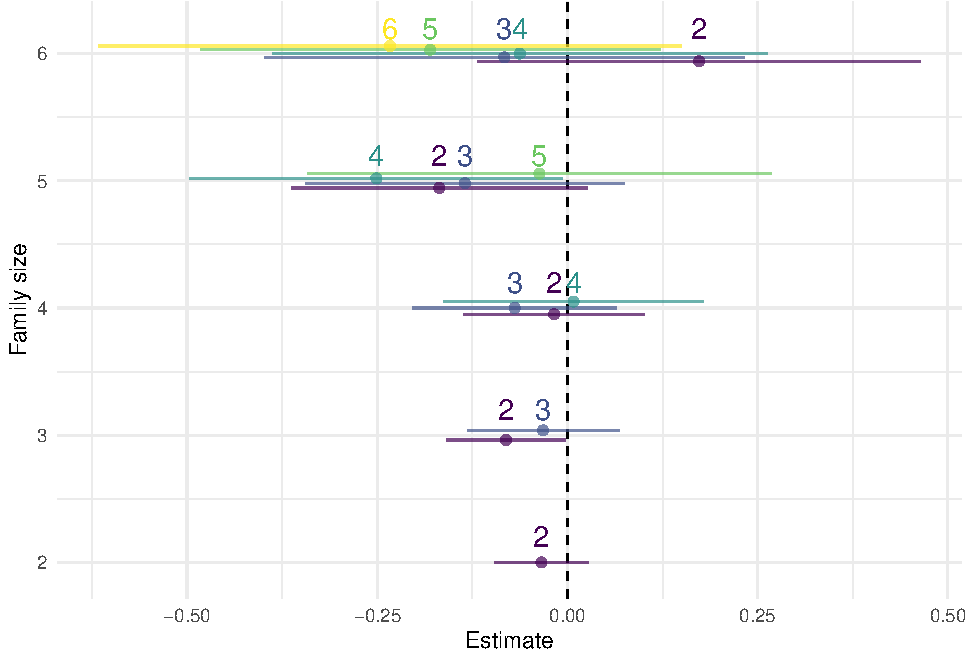
\includegraphics{abdellaoui-borcan-hugh-jones-2021_files/figure-latex/pic-bo-psea-interactions-1} 

}

\caption{Regressions of spouse PSEA: birth order dummies within different family sizes. Labels show birth order. Lines are 95 per cent confidence intervals.}\label{fig:pic-bo-psea-interactions}
\end{figure}

 
  \providecommand{\huxb}[2]{\arrayrulecolor[RGB]{#1}\global\arrayrulewidth=#2pt}
  \providecommand{\huxvb}[2]{\color[RGB]{#1}\vrule width #2pt}
  \providecommand{\huxtpad}[1]{\rule{0pt}{#1}}
  \providecommand{\huxbpad}[1]{\rule[-#1]{0pt}{#1}}

\begin{table}[ht]
\begin{centerbox}
\begin{threeparttable}
\captionsetup{justification=centering,singlelinecheck=off}
\caption{\label{tab:tbl-bo-psea-pgs} Regressions of spouse PSEA with controls for polygenic scores}
 \setlength{\tabcolsep}{0pt}
\begin{tabularx}{1\textwidth}{p{0.2\textwidth} p{0.2\textwidth} p{0.2\textwidth} p{0.2\textwidth} p{0.2\textwidth}}


\hhline{>{\huxb{0, 0, 0}{0.8}}->{\huxb{0, 0, 0}{0.8}}->{\huxb{0, 0, 0}{0.8}}->{\huxb{0, 0, 0}{0.8}}->{\huxb{0, 0, 0}{0.8}}-}
\arrayrulecolor{black}

\multicolumn{1}{!{\huxvb{0, 0, 0}{0}}p{0.2\textwidth}!{\huxvb{0, 0, 0}{0}}}{\hspace{6pt}\parbox[b]{0.2\textwidth-6pt-6pt}{\huxtpad{6pt + 1em}\centering \huxbpad{6pt}}} &
\multicolumn{1}{p{0.2\textwidth}!{\huxvb{0, 0, 0}{0}}}{\hspace{6pt}\parbox[b]{0.2\textwidth-6pt-6pt}{\huxtpad{6pt + 1em}\centering (1)\huxbpad{6pt}}} &
\multicolumn{1}{p{0.2\textwidth}!{\huxvb{0, 0, 0}{0}}}{\hspace{6pt}\parbox[b]{0.2\textwidth-6pt-6pt}{\huxtpad{6pt + 1em}\centering (2)\huxbpad{6pt}}} &
\multicolumn{1}{p{0.2\textwidth}!{\huxvb{0, 0, 0}{0}}}{\hspace{6pt}\parbox[b]{0.2\textwidth-6pt-6pt}{\huxtpad{6pt + 1em}\centering (3)\huxbpad{6pt}}} &
\multicolumn{1}{p{0.2\textwidth}!{\huxvb{0, 0, 0}{0}}}{\hspace{6pt}\parbox[b]{0.2\textwidth-6pt-6pt}{\huxtpad{6pt + 1em}\centering (4)\huxbpad{6pt}}} \tabularnewline[-0.5pt]


\hhline{>{\huxb{255, 255, 255}{0.4}}->{\huxb{0, 0, 0}{0.4}}->{\huxb{0, 0, 0}{0.4}}->{\huxb{0, 0, 0}{0.4}}->{\huxb{0, 0, 0}{0.4}}-}
\arrayrulecolor{black}

\multicolumn{1}{!{\huxvb{0, 0, 0}{0}}p{0.2\textwidth}!{\huxvb{0, 0, 0}{0}}}{\hspace{6pt}\parbox[b]{0.2\textwidth-6pt-6pt}{\huxtpad{6pt + 1em}\raggedright Birth order\huxbpad{6pt}}} &
\multicolumn{1}{p{0.2\textwidth}!{\huxvb{0, 0, 0}{0}}}{\hspace{6pt}\parbox[b]{0.2\textwidth-6pt-6pt}{\huxtpad{6pt + 1em}\raggedleft $-$0.0311~~~~\huxbpad{6pt}}} &
\multicolumn{1}{p{0.2\textwidth}!{\huxvb{0, 0, 0}{0}}}{\hspace{6pt}\parbox[b]{0.2\textwidth-6pt-6pt}{\huxtpad{6pt + 1em}\raggedleft $-$0.0065~~~~\huxbpad{6pt}}} &
\multicolumn{1}{p{0.2\textwidth}!{\huxvb{0, 0, 0}{0}}}{\hspace{6pt}\parbox[b]{0.2\textwidth-6pt-6pt}{\huxtpad{6pt + 1em}\raggedleft $-$0.0132~~~~\huxbpad{6pt}}} &
\multicolumn{1}{p{0.2\textwidth}!{\huxvb{0, 0, 0}{0}}}{\hspace{6pt}\parbox[b]{0.2\textwidth-6pt-6pt}{\huxtpad{6pt + 1em}\raggedleft $-$0.0063~~~~\huxbpad{6pt}}} \tabularnewline[-0.5pt]


\hhline{}
\arrayrulecolor{black}

\multicolumn{1}{!{\huxvb{0, 0, 0}{0}}p{0.2\textwidth}!{\huxvb{0, 0, 0}{0}}}{\hspace{6pt}\parbox[b]{0.2\textwidth-6pt-6pt}{\huxtpad{6pt + 1em}\raggedright \huxbpad{6pt}}} &
\multicolumn{1}{p{0.2\textwidth}!{\huxvb{0, 0, 0}{0}}}{\hspace{6pt}\parbox[b]{0.2\textwidth-6pt-6pt}{\huxtpad{6pt + 1em}\raggedleft (0.0181)~~~\huxbpad{6pt}}} &
\multicolumn{1}{p{0.2\textwidth}!{\huxvb{0, 0, 0}{0}}}{\hspace{6pt}\parbox[b]{0.2\textwidth-6pt-6pt}{\huxtpad{6pt + 1em}\raggedleft (0.0177)~~~\huxbpad{6pt}}} &
\multicolumn{1}{p{0.2\textwidth}!{\huxvb{0, 0, 0}{0}}}{\hspace{6pt}\parbox[b]{0.2\textwidth-6pt-6pt}{\huxtpad{6pt + 1em}\raggedleft (0.0311)~~~\huxbpad{6pt}}} &
\multicolumn{1}{p{0.2\textwidth}!{\huxvb{0, 0, 0}{0}}}{\hspace{6pt}\parbox[b]{0.2\textwidth-6pt-6pt}{\huxtpad{6pt + 1em}\raggedleft (0.0307)~~~\huxbpad{6pt}}} \tabularnewline[-0.5pt]


\hhline{}
\arrayrulecolor{black}

\multicolumn{1}{!{\huxvb{0, 0, 0}{0}}p{0.2\textwidth}!{\huxvb{0, 0, 0}{0}}}{\hspace{6pt}\parbox[b]{0.2\textwidth-6pt-6pt}{\huxtpad{6pt + 1em}\raggedright University\huxbpad{6pt}}} &
\multicolumn{1}{p{0.2\textwidth}!{\huxvb{0, 0, 0}{0}}}{\hspace{6pt}\parbox[b]{0.2\textwidth-6pt-6pt}{\huxtpad{6pt + 1em}\raggedleft ~~~~~~~~~\huxbpad{6pt}}} &
\multicolumn{1}{p{0.2\textwidth}!{\huxvb{0, 0, 0}{0}}}{\hspace{6pt}\parbox[b]{0.2\textwidth-6pt-6pt}{\huxtpad{6pt + 1em}\raggedleft 0.2276 ***\huxbpad{6pt}}} &
\multicolumn{1}{p{0.2\textwidth}!{\huxvb{0, 0, 0}{0}}}{\hspace{6pt}\parbox[b]{0.2\textwidth-6pt-6pt}{\huxtpad{6pt + 1em}\raggedleft ~~~~~~~~~\huxbpad{6pt}}} &
\multicolumn{1}{p{0.2\textwidth}!{\huxvb{0, 0, 0}{0}}}{\hspace{6pt}\parbox[b]{0.2\textwidth-6pt-6pt}{\huxtpad{6pt + 1em}\raggedleft 0.1590 ***\huxbpad{6pt}}} \tabularnewline[-0.5pt]


\hhline{}
\arrayrulecolor{black}

\multicolumn{1}{!{\huxvb{0, 0, 0}{0}}p{0.2\textwidth}!{\huxvb{0, 0, 0}{0}}}{\hspace{6pt}\parbox[b]{0.2\textwidth-6pt-6pt}{\huxtpad{6pt + 1em}\raggedright \huxbpad{6pt}}} &
\multicolumn{1}{p{0.2\textwidth}!{\huxvb{0, 0, 0}{0}}}{\hspace{6pt}\parbox[b]{0.2\textwidth-6pt-6pt}{\huxtpad{6pt + 1em}\raggedleft ~~~~~~~~~\huxbpad{6pt}}} &
\multicolumn{1}{p{0.2\textwidth}!{\huxvb{0, 0, 0}{0}}}{\hspace{6pt}\parbox[b]{0.2\textwidth-6pt-6pt}{\huxtpad{6pt + 1em}\raggedleft (0.0259)~~~\huxbpad{6pt}}} &
\multicolumn{1}{p{0.2\textwidth}!{\huxvb{0, 0, 0}{0}}}{\hspace{6pt}\parbox[b]{0.2\textwidth-6pt-6pt}{\huxtpad{6pt + 1em}\raggedleft ~~~~~~~~~\huxbpad{6pt}}} &
\multicolumn{1}{p{0.2\textwidth}!{\huxvb{0, 0, 0}{0}}}{\hspace{6pt}\parbox[b]{0.2\textwidth-6pt-6pt}{\huxtpad{6pt + 1em}\raggedleft (0.0258)~~~\huxbpad{6pt}}} \tabularnewline[-0.5pt]


\hhline{}
\arrayrulecolor{black}

\multicolumn{1}{!{\huxvb{0, 0, 0}{0}}p{0.2\textwidth}!{\huxvb{0, 0, 0}{0}}}{\hspace{6pt}\parbox[b]{0.2\textwidth-6pt-6pt}{\huxtpad{6pt + 1em}\raggedright Income\huxbpad{6pt}}} &
\multicolumn{1}{p{0.2\textwidth}!{\huxvb{0, 0, 0}{0}}}{\hspace{6pt}\parbox[b]{0.2\textwidth-6pt-6pt}{\huxtpad{6pt + 1em}\raggedleft ~~~~~~~~~\huxbpad{6pt}}} &
\multicolumn{1}{p{0.2\textwidth}!{\huxvb{0, 0, 0}{0}}}{\hspace{6pt}\parbox[b]{0.2\textwidth-6pt-6pt}{\huxtpad{6pt + 1em}\raggedleft ~~~~~~~~~\huxbpad{6pt}}} &
\multicolumn{1}{p{0.2\textwidth}!{\huxvb{0, 0, 0}{0}}}{\hspace{6pt}\parbox[b]{0.2\textwidth-6pt-6pt}{\huxtpad{6pt + 1em}\raggedleft 0.0037 ***\huxbpad{6pt}}} &
\multicolumn{1}{p{0.2\textwidth}!{\huxvb{0, 0, 0}{0}}}{\hspace{6pt}\parbox[b]{0.2\textwidth-6pt-6pt}{\huxtpad{6pt + 1em}\raggedleft 0.0030 ***\huxbpad{6pt}}} \tabularnewline[-0.5pt]


\hhline{}
\arrayrulecolor{black}

\multicolumn{1}{!{\huxvb{0, 0, 0}{0}}p{0.2\textwidth}!{\huxvb{0, 0, 0}{0}}}{\hspace{6pt}\parbox[b]{0.2\textwidth-6pt-6pt}{\huxtpad{6pt + 1em}\raggedright \huxbpad{6pt}}} &
\multicolumn{1}{p{0.2\textwidth}!{\huxvb{0, 0, 0}{0}}}{\hspace{6pt}\parbox[b]{0.2\textwidth-6pt-6pt}{\huxtpad{6pt + 1em}\raggedleft ~~~~~~~~~\huxbpad{6pt}}} &
\multicolumn{1}{p{0.2\textwidth}!{\huxvb{0, 0, 0}{0}}}{\hspace{6pt}\parbox[b]{0.2\textwidth-6pt-6pt}{\huxtpad{6pt + 1em}\raggedleft ~~~~~~~~~\huxbpad{6pt}}} &
\multicolumn{1}{p{0.2\textwidth}!{\huxvb{0, 0, 0}{0}}}{\hspace{6pt}\parbox[b]{0.2\textwidth-6pt-6pt}{\huxtpad{6pt + 1em}\raggedleft (0.0008)~~~\huxbpad{6pt}}} &
\multicolumn{1}{p{0.2\textwidth}!{\huxvb{0, 0, 0}{0}}}{\hspace{6pt}\parbox[b]{0.2\textwidth-6pt-6pt}{\huxtpad{6pt + 1em}\raggedleft (0.0007)~~~\huxbpad{6pt}}} \tabularnewline[-0.5pt]


\hhline{}
\arrayrulecolor{black}

\multicolumn{1}{!{\huxvb{0, 0, 0}{0}}p{0.2\textwidth}!{\huxvb{0, 0, 0}{0}}}{\hspace{6pt}\parbox[b]{0.2\textwidth-6pt-6pt}{\huxtpad{6pt + 1em}\raggedright Own PSEA\huxbpad{6pt}}} &
\multicolumn{1}{p{0.2\textwidth}!{\huxvb{0, 0, 0}{0}}}{\hspace{6pt}\parbox[b]{0.2\textwidth-6pt-6pt}{\huxtpad{6pt + 1em}\raggedleft 0.0529 ***\huxbpad{6pt}}} &
\multicolumn{1}{p{0.2\textwidth}!{\huxvb{0, 0, 0}{0}}}{\hspace{6pt}\parbox[b]{0.2\textwidth-6pt-6pt}{\huxtpad{6pt + 1em}\raggedleft 0.0286 *~~\huxbpad{6pt}}} &
\multicolumn{1}{p{0.2\textwidth}!{\huxvb{0, 0, 0}{0}}}{\hspace{6pt}\parbox[b]{0.2\textwidth-6pt-6pt}{\huxtpad{6pt + 1em}\raggedleft 0.0258~~~~\huxbpad{6pt}}} &
\multicolumn{1}{p{0.2\textwidth}!{\huxvb{0, 0, 0}{0}}}{\hspace{6pt}\parbox[b]{0.2\textwidth-6pt-6pt}{\huxtpad{6pt + 1em}\raggedleft 0.0155~~~~\huxbpad{6pt}}} \tabularnewline[-0.5pt]


\hhline{}
\arrayrulecolor{black}

\multicolumn{1}{!{\huxvb{0, 0, 0}{0}}p{0.2\textwidth}!{\huxvb{0, 0, 0}{0}}}{\hspace{6pt}\parbox[b]{0.2\textwidth-6pt-6pt}{\huxtpad{6pt + 1em}\raggedright \huxbpad{6pt}}} &
\multicolumn{1}{p{0.2\textwidth}!{\huxvb{0, 0, 0}{0}}}{\hspace{6pt}\parbox[b]{0.2\textwidth-6pt-6pt}{\huxtpad{6pt + 1em}\raggedleft (0.0111)~~~\huxbpad{6pt}}} &
\multicolumn{1}{p{0.2\textwidth}!{\huxvb{0, 0, 0}{0}}}{\hspace{6pt}\parbox[b]{0.2\textwidth-6pt-6pt}{\huxtpad{6pt + 1em}\raggedleft (0.0113)~~~\huxbpad{6pt}}} &
\multicolumn{1}{p{0.2\textwidth}!{\huxvb{0, 0, 0}{0}}}{\hspace{6pt}\parbox[b]{0.2\textwidth-6pt-6pt}{\huxtpad{6pt + 1em}\raggedleft (0.0240)~~~\huxbpad{6pt}}} &
\multicolumn{1}{p{0.2\textwidth}!{\huxvb{0, 0, 0}{0}}}{\hspace{6pt}\parbox[b]{0.2\textwidth-6pt-6pt}{\huxtpad{6pt + 1em}\raggedleft (0.0237)~~~\huxbpad{6pt}}} \tabularnewline[-0.5pt]


\hhline{}
\arrayrulecolor{black}

\multicolumn{1}{!{\huxvb{0, 0, 0}{0}}p{0.2\textwidth}!{\huxvb{0, 0, 0}{0}}}{\hspace{6pt}\parbox[b]{0.2\textwidth-6pt-6pt}{\huxtpad{6pt + 1em}\raggedright Parents' age at birth\huxbpad{6pt}}} &
\multicolumn{1}{p{0.2\textwidth}!{\huxvb{0, 0, 0}{0}}}{\hspace{6pt}\parbox[b]{0.2\textwidth-6pt-6pt}{\huxtpad{6pt + 1em}\raggedleft 0.0111 ***\huxbpad{6pt}}} &
\multicolumn{1}{p{0.2\textwidth}!{\huxvb{0, 0, 0}{0}}}{\hspace{6pt}\parbox[b]{0.2\textwidth-6pt-6pt}{\huxtpad{6pt + 1em}\raggedleft 0.0060 *~~\huxbpad{6pt}}} &
\multicolumn{1}{p{0.2\textwidth}!{\huxvb{0, 0, 0}{0}}}{\hspace{6pt}\parbox[b]{0.2\textwidth-6pt-6pt}{\huxtpad{6pt + 1em}\raggedleft 0.0102 *~~\huxbpad{6pt}}} &
\multicolumn{1}{p{0.2\textwidth}!{\huxvb{0, 0, 0}{0}}}{\hspace{6pt}\parbox[b]{0.2\textwidth-6pt-6pt}{\huxtpad{6pt + 1em}\raggedleft 0.0087 *~~\huxbpad{6pt}}} \tabularnewline[-0.5pt]


\hhline{}
\arrayrulecolor{black}

\multicolumn{1}{!{\huxvb{0, 0, 0}{0}}p{0.2\textwidth}!{\huxvb{0, 0, 0}{0}}}{\hspace{6pt}\parbox[b]{0.2\textwidth-6pt-6pt}{\huxtpad{6pt + 1em}\raggedright \huxbpad{6pt}}} &
\multicolumn{1}{p{0.2\textwidth}!{\huxvb{0, 0, 0}{0}}}{\hspace{6pt}\parbox[b]{0.2\textwidth-6pt-6pt}{\huxtpad{6pt + 1em}\raggedleft (0.0028)~~~\huxbpad{6pt}}} &
\multicolumn{1}{p{0.2\textwidth}!{\huxvb{0, 0, 0}{0}}}{\hspace{6pt}\parbox[b]{0.2\textwidth-6pt-6pt}{\huxtpad{6pt + 1em}\raggedleft (0.0028)~~~\huxbpad{6pt}}} &
\multicolumn{1}{p{0.2\textwidth}!{\huxvb{0, 0, 0}{0}}}{\hspace{6pt}\parbox[b]{0.2\textwidth-6pt-6pt}{\huxtpad{6pt + 1em}\raggedleft (0.0040)~~~\huxbpad{6pt}}} &
\multicolumn{1}{p{0.2\textwidth}!{\huxvb{0, 0, 0}{0}}}{\hspace{6pt}\parbox[b]{0.2\textwidth-6pt-6pt}{\huxtpad{6pt + 1em}\raggedleft (0.0041)~~~\huxbpad{6pt}}} \tabularnewline[-0.5pt]


\hhline{}
\arrayrulecolor{black}

\multicolumn{1}{!{\huxvb{0, 0, 0}{0}}p{0.2\textwidth}!{\huxvb{0, 0, 0}{0}}}{\hspace{6pt}\parbox[b]{0.2\textwidth-6pt-6pt}{\huxtpad{6pt + 1em}\raggedright Fluid IQ\huxbpad{6pt}}} &
\multicolumn{1}{p{0.2\textwidth}!{\huxvb{0, 0, 0}{0}}}{\hspace{6pt}\parbox[b]{0.2\textwidth-6pt-6pt}{\huxtpad{6pt + 1em}\raggedleft ~~~~~~~~~\huxbpad{6pt}}} &
\multicolumn{1}{p{0.2\textwidth}!{\huxvb{0, 0, 0}{0}}}{\hspace{6pt}\parbox[b]{0.2\textwidth-6pt-6pt}{\huxtpad{6pt + 1em}\raggedleft 0.0171 *~~\huxbpad{6pt}}} &
\multicolumn{1}{p{0.2\textwidth}!{\huxvb{0, 0, 0}{0}}}{\hspace{6pt}\parbox[b]{0.2\textwidth-6pt-6pt}{\huxtpad{6pt + 1em}\raggedleft 0.0197 +~~\huxbpad{6pt}}} &
\multicolumn{1}{p{0.2\textwidth}!{\huxvb{0, 0, 0}{0}}}{\hspace{6pt}\parbox[b]{0.2\textwidth-6pt-6pt}{\huxtpad{6pt + 1em}\raggedleft 0.0104~~~~\huxbpad{6pt}}} \tabularnewline[-0.5pt]


\hhline{}
\arrayrulecolor{black}

\multicolumn{1}{!{\huxvb{0, 0, 0}{0}}p{0.2\textwidth}!{\huxvb{0, 0, 0}{0}}}{\hspace{6pt}\parbox[b]{0.2\textwidth-6pt-6pt}{\huxtpad{6pt + 1em}\raggedright \huxbpad{6pt}}} &
\multicolumn{1}{p{0.2\textwidth}!{\huxvb{0, 0, 0}{0}}}{\hspace{6pt}\parbox[b]{0.2\textwidth-6pt-6pt}{\huxtpad{6pt + 1em}\raggedleft ~~~~~~~~~\huxbpad{6pt}}} &
\multicolumn{1}{p{0.2\textwidth}!{\huxvb{0, 0, 0}{0}}}{\hspace{6pt}\parbox[b]{0.2\textwidth-6pt-6pt}{\huxtpad{6pt + 1em}\raggedleft (0.0065)~~~\huxbpad{6pt}}} &
\multicolumn{1}{p{0.2\textwidth}!{\huxvb{0, 0, 0}{0}}}{\hspace{6pt}\parbox[b]{0.2\textwidth-6pt-6pt}{\huxtpad{6pt + 1em}\raggedleft (0.0112)~~~\huxbpad{6pt}}} &
\multicolumn{1}{p{0.2\textwidth}!{\huxvb{0, 0, 0}{0}}}{\hspace{6pt}\parbox[b]{0.2\textwidth-6pt-6pt}{\huxtpad{6pt + 1em}\raggedleft (0.0118)~~~\huxbpad{6pt}}} \tabularnewline[-0.5pt]


\hhline{}
\arrayrulecolor{black}

\multicolumn{1}{!{\huxvb{0, 0, 0}{0}}p{0.2\textwidth}!{\huxvb{0, 0, 0}{0}}}{\hspace{6pt}\parbox[b]{0.2\textwidth-6pt-6pt}{\huxtpad{6pt + 1em}\raggedright Height\huxbpad{6pt}}} &
\multicolumn{1}{p{0.2\textwidth}!{\huxvb{0, 0, 0}{0}}}{\hspace{6pt}\parbox[b]{0.2\textwidth-6pt-6pt}{\huxtpad{6pt + 1em}\raggedleft ~~~~~~~~~\huxbpad{6pt}}} &
\multicolumn{1}{p{0.2\textwidth}!{\huxvb{0, 0, 0}{0}}}{\hspace{6pt}\parbox[b]{0.2\textwidth-6pt-6pt}{\huxtpad{6pt + 1em}\raggedleft 0.0027 *~~\huxbpad{6pt}}} &
\multicolumn{1}{p{0.2\textwidth}!{\huxvb{0, 0, 0}{0}}}{\hspace{6pt}\parbox[b]{0.2\textwidth-6pt-6pt}{\huxtpad{6pt + 1em}\raggedleft 0.0046 *~~\huxbpad{6pt}}} &
\multicolumn{1}{p{0.2\textwidth}!{\huxvb{0, 0, 0}{0}}}{\hspace{6pt}\parbox[b]{0.2\textwidth-6pt-6pt}{\huxtpad{6pt + 1em}\raggedleft 0.0042 *~~\huxbpad{6pt}}} \tabularnewline[-0.5pt]


\hhline{}
\arrayrulecolor{black}

\multicolumn{1}{!{\huxvb{0, 0, 0}{0}}p{0.2\textwidth}!{\huxvb{0, 0, 0}{0}}}{\hspace{6pt}\parbox[b]{0.2\textwidth-6pt-6pt}{\huxtpad{6pt + 1em}\raggedright \huxbpad{6pt}}} &
\multicolumn{1}{p{0.2\textwidth}!{\huxvb{0, 0, 0}{0}}}{\hspace{6pt}\parbox[b]{0.2\textwidth-6pt-6pt}{\huxtpad{6pt + 1em}\raggedleft ~~~~~~~~~\huxbpad{6pt}}} &
\multicolumn{1}{p{0.2\textwidth}!{\huxvb{0, 0, 0}{0}}}{\hspace{6pt}\parbox[b]{0.2\textwidth-6pt-6pt}{\huxtpad{6pt + 1em}\raggedleft (0.0011)~~~\huxbpad{6pt}}} &
\multicolumn{1}{p{0.2\textwidth}!{\huxvb{0, 0, 0}{0}}}{\hspace{6pt}\parbox[b]{0.2\textwidth-6pt-6pt}{\huxtpad{6pt + 1em}\raggedleft (0.0018)~~~\huxbpad{6pt}}} &
\multicolumn{1}{p{0.2\textwidth}!{\huxvb{0, 0, 0}{0}}}{\hspace{6pt}\parbox[b]{0.2\textwidth-6pt-6pt}{\huxtpad{6pt + 1em}\raggedleft (0.0018)~~~\huxbpad{6pt}}} \tabularnewline[-0.5pt]


\hhline{>{\huxb{255, 255, 255}{0.4}}->{\huxb{0, 0, 0}{0.4}}->{\huxb{0, 0, 0}{0.4}}->{\huxb{0, 0, 0}{0.4}}->{\huxb{0, 0, 0}{0.4}}-}
\arrayrulecolor{black}

\multicolumn{1}{!{\huxvb{0, 0, 0}{0}}p{0.2\textwidth}!{\huxvb{0, 0, 0}{0}}}{\hspace{6pt}\parbox[b]{0.2\textwidth-6pt-6pt}{\huxtpad{6pt + 1em}\raggedright Family size dummies\huxbpad{6pt}}} &
\multicolumn{1}{p{0.2\textwidth}!{\huxvb{0, 0, 0}{0}}}{\hspace{6pt}\parbox[b]{0.2\textwidth-6pt-6pt}{\huxtpad{6pt + 1em}\centering Yes\huxbpad{6pt}}} &
\multicolumn{1}{p{0.2\textwidth}!{\huxvb{0, 0, 0}{0}}}{\hspace{6pt}\parbox[b]{0.2\textwidth-6pt-6pt}{\huxtpad{6pt + 1em}\centering Yes\huxbpad{6pt}}} &
\multicolumn{1}{p{0.2\textwidth}!{\huxvb{0, 0, 0}{0}}}{\hspace{6pt}\parbox[b]{0.2\textwidth-6pt-6pt}{\huxtpad{6pt + 1em}\centering Yes\huxbpad{6pt}}} &
\multicolumn{1}{p{0.2\textwidth}!{\huxvb{0, 0, 0}{0}}}{\hspace{6pt}\parbox[b]{0.2\textwidth-6pt-6pt}{\huxtpad{6pt + 1em}\centering Yes\huxbpad{6pt}}} \tabularnewline[-0.5pt]


\hhline{}
\arrayrulecolor{black}

\multicolumn{1}{!{\huxvb{0, 0, 0}{0}}p{0.2\textwidth}!{\huxvb{0, 0, 0}{0}}}{\hspace{6pt}\parbox[b]{0.2\textwidth-6pt-6pt}{\huxtpad{6pt + 1em}\raggedright Birth month dummies\huxbpad{6pt}}} &
\multicolumn{1}{p{0.2\textwidth}!{\huxvb{0, 0, 0}{0}}}{\hspace{6pt}\parbox[b]{0.2\textwidth-6pt-6pt}{\huxtpad{6pt + 1em}\centering Yes\huxbpad{6pt}}} &
\multicolumn{1}{p{0.2\textwidth}!{\huxvb{0, 0, 0}{0}}}{\hspace{6pt}\parbox[b]{0.2\textwidth-6pt-6pt}{\huxtpad{6pt + 1em}\centering Yes\huxbpad{6pt}}} &
\multicolumn{1}{p{0.2\textwidth}!{\huxvb{0, 0, 0}{0}}}{\hspace{6pt}\parbox[b]{0.2\textwidth-6pt-6pt}{\huxtpad{6pt + 1em}\centering Yes\huxbpad{6pt}}} &
\multicolumn{1}{p{0.2\textwidth}!{\huxvb{0, 0, 0}{0}}}{\hspace{6pt}\parbox[b]{0.2\textwidth-6pt-6pt}{\huxtpad{6pt + 1em}\centering Yes\huxbpad{6pt}}} \tabularnewline[-0.5pt]


\hhline{}
\arrayrulecolor{black}

\multicolumn{1}{!{\huxvb{0, 0, 0}{0}}p{0.2\textwidth}!{\huxvb{0, 0, 0}{0}}}{\hspace{6pt}\parbox[b]{0.2\textwidth-6pt-6pt}{\huxtpad{6pt + 1em}\raggedright Birth year dummies\huxbpad{6pt}}} &
\multicolumn{1}{p{0.2\textwidth}!{\huxvb{0, 0, 0}{0}}}{\hspace{6pt}\parbox[b]{0.2\textwidth-6pt-6pt}{\huxtpad{6pt + 1em}\centering Yes\huxbpad{6pt}}} &
\multicolumn{1}{p{0.2\textwidth}!{\huxvb{0, 0, 0}{0}}}{\hspace{6pt}\parbox[b]{0.2\textwidth-6pt-6pt}{\huxtpad{6pt + 1em}\centering Yes\huxbpad{6pt}}} &
\multicolumn{1}{p{0.2\textwidth}!{\huxvb{0, 0, 0}{0}}}{\hspace{6pt}\parbox[b]{0.2\textwidth-6pt-6pt}{\huxtpad{6pt + 1em}\centering Yes\huxbpad{6pt}}} &
\multicolumn{1}{p{0.2\textwidth}!{\huxvb{0, 0, 0}{0}}}{\hspace{6pt}\parbox[b]{0.2\textwidth-6pt-6pt}{\huxtpad{6pt + 1em}\centering Yes\huxbpad{6pt}}} \tabularnewline[-0.5pt]


\hhline{}
\arrayrulecolor{black}

\multicolumn{1}{!{\huxvb{0, 0, 0}{0}}p{0.2\textwidth}!{\huxvb{0, 0, 0}{0}}}{\hspace{6pt}\parbox[b]{0.2\textwidth-6pt-6pt}{\huxtpad{6pt + 1em}\raggedright Polygenic score controls\huxbpad{6pt}}} &
\multicolumn{1}{p{0.2\textwidth}!{\huxvb{0, 0, 0}{0}}}{\hspace{6pt}\parbox[b]{0.2\textwidth-6pt-6pt}{\huxtpad{6pt + 1em}\centering Yes\huxbpad{6pt}}} &
\multicolumn{1}{p{0.2\textwidth}!{\huxvb{0, 0, 0}{0}}}{\hspace{6pt}\parbox[b]{0.2\textwidth-6pt-6pt}{\huxtpad{6pt + 1em}\centering Yes\huxbpad{6pt}}} &
\multicolumn{1}{p{0.2\textwidth}!{\huxvb{0, 0, 0}{0}}}{\hspace{6pt}\parbox[b]{0.2\textwidth-6pt-6pt}{\huxtpad{6pt + 1em}\centering Yes\huxbpad{6pt}}} &
\multicolumn{1}{p{0.2\textwidth}!{\huxvb{0, 0, 0}{0}}}{\hspace{6pt}\parbox[b]{0.2\textwidth-6pt-6pt}{\huxtpad{6pt + 1em}\centering Yes\huxbpad{6pt}}} \tabularnewline[-0.5pt]


\hhline{>{\huxb{255, 255, 255}{0.4}}->{\huxb{0, 0, 0}{0.4}}->{\huxb{0, 0, 0}{0.4}}->{\huxb{0, 0, 0}{0.4}}->{\huxb{0, 0, 0}{0.4}}-}
\arrayrulecolor{black}

\multicolumn{1}{!{\huxvb{0, 0, 0}{0}}p{0.2\textwidth}!{\huxvb{0, 0, 0}{0}}}{\hspace{6pt}\parbox[b]{0.2\textwidth-6pt-6pt}{\huxtpad{6pt + 1em}\raggedright N\huxbpad{6pt}}} &
\multicolumn{1}{p{0.2\textwidth}!{\huxvb{0, 0, 0}{0}}}{\hspace{6pt}\parbox[b]{0.2\textwidth-6pt-6pt}{\huxtpad{6pt + 1em}\raggedleft 10229~~~~~~~~~\huxbpad{6pt}}} &
\multicolumn{1}{p{0.2\textwidth}!{\huxvb{0, 0, 0}{0}}}{\hspace{6pt}\parbox[b]{0.2\textwidth-6pt-6pt}{\huxtpad{6pt + 1em}\raggedleft 10229~~~~~~~~~\huxbpad{6pt}}} &
\multicolumn{1}{p{0.2\textwidth}!{\huxvb{0, 0, 0}{0}}}{\hspace{6pt}\parbox[b]{0.2\textwidth-6pt-6pt}{\huxtpad{6pt + 1em}\raggedleft 3414~~~~~~~~~\huxbpad{6pt}}} &
\multicolumn{1}{p{0.2\textwidth}!{\huxvb{0, 0, 0}{0}}}{\hspace{6pt}\parbox[b]{0.2\textwidth-6pt-6pt}{\huxtpad{6pt + 1em}\raggedleft 3414~~~~~~~~~\huxbpad{6pt}}} \tabularnewline[-0.5pt]


\hhline{}
\arrayrulecolor{black}

\multicolumn{1}{!{\huxvb{0, 0, 0}{0}}p{0.2\textwidth}!{\huxvb{0, 0, 0}{0}}}{\hspace{6pt}\parbox[b]{0.2\textwidth-6pt-6pt}{\huxtpad{6pt + 1em}\raggedright R2\huxbpad{6pt}}} &
\multicolumn{1}{p{0.2\textwidth}!{\huxvb{0, 0, 0}{0}}}{\hspace{6pt}\parbox[b]{0.2\textwidth-6pt-6pt}{\huxtpad{6pt + 1em}\raggedleft 0.014~~~~~\huxbpad{6pt}}} &
\multicolumn{1}{p{0.2\textwidth}!{\huxvb{0, 0, 0}{0}}}{\hspace{6pt}\parbox[b]{0.2\textwidth-6pt-6pt}{\huxtpad{6pt + 1em}\raggedleft 0.030~~~~~\huxbpad{6pt}}} &
\multicolumn{1}{p{0.2\textwidth}!{\huxvb{0, 0, 0}{0}}}{\hspace{6pt}\parbox[b]{0.2\textwidth-6pt-6pt}{\huxtpad{6pt + 1em}\raggedleft 0.028~~~~~\huxbpad{6pt}}} &
\multicolumn{1}{p{0.2\textwidth}!{\huxvb{0, 0, 0}{0}}}{\hspace{6pt}\parbox[b]{0.2\textwidth-6pt-6pt}{\huxtpad{6pt + 1em}\raggedleft 0.033~~~~~\huxbpad{6pt}}} \tabularnewline[-0.5pt]


\hhline{>{\huxb{0, 0, 0}{0.8}}->{\huxb{0, 0, 0}{0.8}}->{\huxb{0, 0, 0}{0.8}}->{\huxb{0, 0, 0}{0.8}}->{\huxb{0, 0, 0}{0.8}}-}
\arrayrulecolor{black}

\multicolumn{5}{!{\huxvb{0, 0, 0}{0}}p{1\textwidth+8\tabcolsep}!{\huxvb{0, 0, 0}{0}}}{\hspace{6pt}\parbox[b]{1\textwidth+8\tabcolsep-6pt-6pt}{\huxtpad{6pt + 1em}\raggedright  *** p $<$ 0.001;  ** p $<$ 0.01;  * p $<$ 0.05;  + p $<$ 0.1. Standard errors: robust.  \newline Polygenic scores: alzheimer's, caffeine, cognitive ability, neuroticism, substance use.\huxbpad{6pt}}} \tabularnewline[-0.5pt]


\hhline{}
\arrayrulecolor{black}
\end{tabularx}
\end{threeparttable}\par\end{centerbox}

\end{table}
 

 
  \providecommand{\huxb}[2]{\arrayrulecolor[RGB]{#1}\global\arrayrulewidth=#2pt}
  \providecommand{\huxvb}[2]{\color[RGB]{#1}\vrule width #2pt}
  \providecommand{\huxtpad}[1]{\rule{0pt}{#1}}
  \providecommand{\huxbpad}[1]{\rule[-#1]{0pt}{#1}}

\begin{table}[ht]
\begin{centerbox}
\begin{threeparttable}
\captionsetup{justification=centering,singlelinecheck=off}
\caption{\label{tab:tbl-bo-psea-age-fte} Regressions of spouse PSEA using age of leaving full-time education}
 \setlength{\tabcolsep}{0pt}
\begin{tabularx}{0.8\textwidth}{p{0.2\textwidth} p{0.2\textwidth} p{0.2\textwidth} p{0.2\textwidth}}


\hhline{>{\huxb{0, 0, 0}{0.8}}->{\huxb{0, 0, 0}{0.8}}->{\huxb{0, 0, 0}{0.8}}->{\huxb{0, 0, 0}{0.8}}-}
\arrayrulecolor{black}

\multicolumn{1}{!{\huxvb{0, 0, 0}{0}}p{0.2\textwidth}!{\huxvb{0, 0, 0}{0}}}{\hspace{6pt}\parbox[b]{0.2\textwidth-6pt-6pt}{\huxtpad{6pt + 1em}\centering \huxbpad{6pt}}} &
\multicolumn{1}{p{0.2\textwidth}!{\huxvb{0, 0, 0}{0}}}{\hspace{6pt}\parbox[b]{0.2\textwidth-6pt-6pt}{\huxtpad{6pt + 1em}\centering (1)\huxbpad{6pt}}} &
\multicolumn{1}{p{0.2\textwidth}!{\huxvb{0, 0, 0}{0}}}{\hspace{6pt}\parbox[b]{0.2\textwidth-6pt-6pt}{\huxtpad{6pt + 1em}\centering (2)\huxbpad{6pt}}} &
\multicolumn{1}{p{0.2\textwidth}!{\huxvb{0, 0, 0}{0}}}{\hspace{6pt}\parbox[b]{0.2\textwidth-6pt-6pt}{\huxtpad{6pt + 1em}\centering (3)\huxbpad{6pt}}} \tabularnewline[-0.5pt]


\hhline{>{\huxb{255, 255, 255}{0.4}}->{\huxb{0, 0, 0}{0.4}}->{\huxb{0, 0, 0}{0.4}}->{\huxb{0, 0, 0}{0.4}}-}
\arrayrulecolor{black}

\multicolumn{1}{!{\huxvb{0, 0, 0}{0}}p{0.2\textwidth}!{\huxvb{0, 0, 0}{0}}}{\hspace{6pt}\parbox[b]{0.2\textwidth-6pt-6pt}{\huxtpad{6pt + 1em}\raggedright Birth order\huxbpad{6pt}}} &
\multicolumn{1}{p{0.2\textwidth}!{\huxvb{0, 0, 0}{0}}}{\hspace{6pt}\parbox[b]{0.2\textwidth-6pt-6pt}{\huxtpad{6pt + 1em}\raggedleft $-$0.0312 *~~\huxbpad{6pt}}} &
\multicolumn{1}{p{0.2\textwidth}!{\huxvb{0, 0, 0}{0}}}{\hspace{6pt}\parbox[b]{0.2\textwidth-6pt-6pt}{\huxtpad{6pt + 1em}\raggedleft 0.0005~~~~\huxbpad{6pt}}} &
\multicolumn{1}{p{0.2\textwidth}!{\huxvb{0, 0, 0}{0}}}{\hspace{6pt}\parbox[b]{0.2\textwidth-6pt-6pt}{\huxtpad{6pt + 1em}\raggedleft 0.0018~~~~\huxbpad{6pt}}} \tabularnewline[-0.5pt]


\hhline{}
\arrayrulecolor{black}

\multicolumn{1}{!{\huxvb{0, 0, 0}{0}}p{0.2\textwidth}!{\huxvb{0, 0, 0}{0}}}{\hspace{6pt}\parbox[b]{0.2\textwidth-6pt-6pt}{\huxtpad{6pt + 1em}\raggedright \huxbpad{6pt}}} &
\multicolumn{1}{p{0.2\textwidth}!{\huxvb{0, 0, 0}{0}}}{\hspace{6pt}\parbox[b]{0.2\textwidth-6pt-6pt}{\huxtpad{6pt + 1em}\raggedleft (0.0146)~~~\huxbpad{6pt}}} &
\multicolumn{1}{p{0.2\textwidth}!{\huxvb{0, 0, 0}{0}}}{\hspace{6pt}\parbox[b]{0.2\textwidth-6pt-6pt}{\huxtpad{6pt + 1em}\raggedleft (0.0147)~~~\huxbpad{6pt}}} &
\multicolumn{1}{p{0.2\textwidth}!{\huxvb{0, 0, 0}{0}}}{\hspace{6pt}\parbox[b]{0.2\textwidth-6pt-6pt}{\huxtpad{6pt + 1em}\raggedleft (0.0270)~~~\huxbpad{6pt}}} \tabularnewline[-0.5pt]


\hhline{}
\arrayrulecolor{black}

\multicolumn{1}{!{\huxvb{0, 0, 0}{0}}p{0.2\textwidth}!{\huxvb{0, 0, 0}{0}}}{\hspace{6pt}\parbox[b]{0.2\textwidth-6pt-6pt}{\huxtpad{6pt + 1em}\raggedright Age left full-time educ.\huxbpad{6pt}}} &
\multicolumn{1}{p{0.2\textwidth}!{\huxvb{0, 0, 0}{0}}}{\hspace{6pt}\parbox[b]{0.2\textwidth-6pt-6pt}{\huxtpad{6pt + 1em}\raggedleft ~~~~~~~~~\huxbpad{6pt}}} &
\multicolumn{1}{p{0.2\textwidth}!{\huxvb{0, 0, 0}{0}}}{\hspace{6pt}\parbox[b]{0.2\textwidth-6pt-6pt}{\huxtpad{6pt + 1em}\raggedleft 0.0497 ***\huxbpad{6pt}}} &
\multicolumn{1}{p{0.2\textwidth}!{\huxvb{0, 0, 0}{0}}}{\hspace{6pt}\parbox[b]{0.2\textwidth-6pt-6pt}{\huxtpad{6pt + 1em}\raggedleft 0.0417 ***\huxbpad{6pt}}} \tabularnewline[-0.5pt]


\hhline{}
\arrayrulecolor{black}

\multicolumn{1}{!{\huxvb{0, 0, 0}{0}}p{0.2\textwidth}!{\huxvb{0, 0, 0}{0}}}{\hspace{6pt}\parbox[b]{0.2\textwidth-6pt-6pt}{\huxtpad{6pt + 1em}\raggedright \huxbpad{6pt}}} &
\multicolumn{1}{p{0.2\textwidth}!{\huxvb{0, 0, 0}{0}}}{\hspace{6pt}\parbox[b]{0.2\textwidth-6pt-6pt}{\huxtpad{6pt + 1em}\raggedleft ~~~~~~~~~\huxbpad{6pt}}} &
\multicolumn{1}{p{0.2\textwidth}!{\huxvb{0, 0, 0}{0}}}{\hspace{6pt}\parbox[b]{0.2\textwidth-6pt-6pt}{\huxtpad{6pt + 1em}\raggedleft (0.0044)~~~\huxbpad{6pt}}} &
\multicolumn{1}{p{0.2\textwidth}!{\huxvb{0, 0, 0}{0}}}{\hspace{6pt}\parbox[b]{0.2\textwidth-6pt-6pt}{\huxtpad{6pt + 1em}\raggedleft (0.0078)~~~\huxbpad{6pt}}} \tabularnewline[-0.5pt]


\hhline{}
\arrayrulecolor{black}

\multicolumn{1}{!{\huxvb{0, 0, 0}{0}}p{0.2\textwidth}!{\huxvb{0, 0, 0}{0}}}{\hspace{6pt}\parbox[b]{0.2\textwidth-6pt-6pt}{\huxtpad{6pt + 1em}\raggedright Income\huxbpad{6pt}}} &
\multicolumn{1}{p{0.2\textwidth}!{\huxvb{0, 0, 0}{0}}}{\hspace{6pt}\parbox[b]{0.2\textwidth-6pt-6pt}{\huxtpad{6pt + 1em}\raggedleft ~~~~~~~~~\huxbpad{6pt}}} &
\multicolumn{1}{p{0.2\textwidth}!{\huxvb{0, 0, 0}{0}}}{\hspace{6pt}\parbox[b]{0.2\textwidth-6pt-6pt}{\huxtpad{6pt + 1em}\raggedleft ~~~~~~~~~\huxbpad{6pt}}} &
\multicolumn{1}{p{0.2\textwidth}!{\huxvb{0, 0, 0}{0}}}{\hspace{6pt}\parbox[b]{0.2\textwidth-6pt-6pt}{\huxtpad{6pt + 1em}\raggedleft 0.0028 *~~\huxbpad{6pt}}} \tabularnewline[-0.5pt]


\hhline{}
\arrayrulecolor{black}

\multicolumn{1}{!{\huxvb{0, 0, 0}{0}}p{0.2\textwidth}!{\huxvb{0, 0, 0}{0}}}{\hspace{6pt}\parbox[b]{0.2\textwidth-6pt-6pt}{\huxtpad{6pt + 1em}\raggedright \huxbpad{6pt}}} &
\multicolumn{1}{p{0.2\textwidth}!{\huxvb{0, 0, 0}{0}}}{\hspace{6pt}\parbox[b]{0.2\textwidth-6pt-6pt}{\huxtpad{6pt + 1em}\raggedleft ~~~~~~~~~\huxbpad{6pt}}} &
\multicolumn{1}{p{0.2\textwidth}!{\huxvb{0, 0, 0}{0}}}{\hspace{6pt}\parbox[b]{0.2\textwidth-6pt-6pt}{\huxtpad{6pt + 1em}\raggedleft ~~~~~~~~~\huxbpad{6pt}}} &
\multicolumn{1}{p{0.2\textwidth}!{\huxvb{0, 0, 0}{0}}}{\hspace{6pt}\parbox[b]{0.2\textwidth-6pt-6pt}{\huxtpad{6pt + 1em}\raggedleft (0.0011)~~~\huxbpad{6pt}}} \tabularnewline[-0.5pt]


\hhline{}
\arrayrulecolor{black}

\multicolumn{1}{!{\huxvb{0, 0, 0}{0}}p{0.2\textwidth}!{\huxvb{0, 0, 0}{0}}}{\hspace{6pt}\parbox[b]{0.2\textwidth-6pt-6pt}{\huxtpad{6pt + 1em}\raggedright Parents' age at birth\huxbpad{6pt}}} &
\multicolumn{1}{p{0.2\textwidth}!{\huxvb{0, 0, 0}{0}}}{\hspace{6pt}\parbox[b]{0.2\textwidth-6pt-6pt}{\huxtpad{6pt + 1em}\raggedleft 0.0113 ***\huxbpad{6pt}}} &
\multicolumn{1}{p{0.2\textwidth}!{\huxvb{0, 0, 0}{0}}}{\hspace{6pt}\parbox[b]{0.2\textwidth-6pt-6pt}{\huxtpad{6pt + 1em}\raggedleft 0.0049 +~~\huxbpad{6pt}}} &
\multicolumn{1}{p{0.2\textwidth}!{\huxvb{0, 0, 0}{0}}}{\hspace{6pt}\parbox[b]{0.2\textwidth-6pt-6pt}{\huxtpad{6pt + 1em}\raggedleft 0.0071~~~~\huxbpad{6pt}}} \tabularnewline[-0.5pt]


\hhline{}
\arrayrulecolor{black}

\multicolumn{1}{!{\huxvb{0, 0, 0}{0}}p{0.2\textwidth}!{\huxvb{0, 0, 0}{0}}}{\hspace{6pt}\parbox[b]{0.2\textwidth-6pt-6pt}{\huxtpad{6pt + 1em}\raggedright \huxbpad{6pt}}} &
\multicolumn{1}{p{0.2\textwidth}!{\huxvb{0, 0, 0}{0}}}{\hspace{6pt}\parbox[b]{0.2\textwidth-6pt-6pt}{\huxtpad{6pt + 1em}\raggedleft (0.0026)~~~\huxbpad{6pt}}} &
\multicolumn{1}{p{0.2\textwidth}!{\huxvb{0, 0, 0}{0}}}{\hspace{6pt}\parbox[b]{0.2\textwidth-6pt-6pt}{\huxtpad{6pt + 1em}\raggedleft (0.0026)~~~\huxbpad{6pt}}} &
\multicolumn{1}{p{0.2\textwidth}!{\huxvb{0, 0, 0}{0}}}{\hspace{6pt}\parbox[b]{0.2\textwidth-6pt-6pt}{\huxtpad{6pt + 1em}\raggedleft (0.0047)~~~\huxbpad{6pt}}} \tabularnewline[-0.5pt]


\hhline{}
\arrayrulecolor{black}

\multicolumn{1}{!{\huxvb{0, 0, 0}{0}}p{0.2\textwidth}!{\huxvb{0, 0, 0}{0}}}{\hspace{6pt}\parbox[b]{0.2\textwidth-6pt-6pt}{\huxtpad{6pt + 1em}\raggedright Own PSEA\huxbpad{6pt}}} &
\multicolumn{1}{p{0.2\textwidth}!{\huxvb{0, 0, 0}{0}}}{\hspace{6pt}\parbox[b]{0.2\textwidth-6pt-6pt}{\huxtpad{6pt + 1em}\raggedleft 0.0583 ***\huxbpad{6pt}}} &
\multicolumn{1}{p{0.2\textwidth}!{\huxvb{0, 0, 0}{0}}}{\hspace{6pt}\parbox[b]{0.2\textwidth-6pt-6pt}{\huxtpad{6pt + 1em}\raggedleft 0.0305 **~\huxbpad{6pt}}} &
\multicolumn{1}{p{0.2\textwidth}!{\huxvb{0, 0, 0}{0}}}{\hspace{6pt}\parbox[b]{0.2\textwidth-6pt-6pt}{\huxtpad{6pt + 1em}\raggedleft 0.0198~~~~\huxbpad{6pt}}} \tabularnewline[-0.5pt]


\hhline{}
\arrayrulecolor{black}

\multicolumn{1}{!{\huxvb{0, 0, 0}{0}}p{0.2\textwidth}!{\huxvb{0, 0, 0}{0}}}{\hspace{6pt}\parbox[b]{0.2\textwidth-6pt-6pt}{\huxtpad{6pt + 1em}\raggedright \huxbpad{6pt}}} &
\multicolumn{1}{p{0.2\textwidth}!{\huxvb{0, 0, 0}{0}}}{\hspace{6pt}\parbox[b]{0.2\textwidth-6pt-6pt}{\huxtpad{6pt + 1em}\raggedleft (0.0100)~~~\huxbpad{6pt}}} &
\multicolumn{1}{p{0.2\textwidth}!{\huxvb{0, 0, 0}{0}}}{\hspace{6pt}\parbox[b]{0.2\textwidth-6pt-6pt}{\huxtpad{6pt + 1em}\raggedleft (0.0101)~~~\huxbpad{6pt}}} &
\multicolumn{1}{p{0.2\textwidth}!{\huxvb{0, 0, 0}{0}}}{\hspace{6pt}\parbox[b]{0.2\textwidth-6pt-6pt}{\huxtpad{6pt + 1em}\raggedleft (0.0185)~~~\huxbpad{6pt}}} \tabularnewline[-0.5pt]


\hhline{}
\arrayrulecolor{black}

\multicolumn{1}{!{\huxvb{0, 0, 0}{0}}p{0.2\textwidth}!{\huxvb{0, 0, 0}{0}}}{\hspace{6pt}\parbox[b]{0.2\textwidth-6pt-6pt}{\huxtpad{6pt + 1em}\raggedright Fluid IQ\huxbpad{6pt}}} &
\multicolumn{1}{p{0.2\textwidth}!{\huxvb{0, 0, 0}{0}}}{\hspace{6pt}\parbox[b]{0.2\textwidth-6pt-6pt}{\huxtpad{6pt + 1em}\raggedleft ~~~~~~~~~\huxbpad{6pt}}} &
\multicolumn{1}{p{0.2\textwidth}!{\huxvb{0, 0, 0}{0}}}{\hspace{6pt}\parbox[b]{0.2\textwidth-6pt-6pt}{\huxtpad{6pt + 1em}\raggedleft 0.0143 **~\huxbpad{6pt}}} &
\multicolumn{1}{p{0.2\textwidth}!{\huxvb{0, 0, 0}{0}}}{\hspace{6pt}\parbox[b]{0.2\textwidth-6pt-6pt}{\huxtpad{6pt + 1em}\raggedleft 0.0068~~~~\huxbpad{6pt}}} \tabularnewline[-0.5pt]


\hhline{}
\arrayrulecolor{black}

\multicolumn{1}{!{\huxvb{0, 0, 0}{0}}p{0.2\textwidth}!{\huxvb{0, 0, 0}{0}}}{\hspace{6pt}\parbox[b]{0.2\textwidth-6pt-6pt}{\huxtpad{6pt + 1em}\raggedright \huxbpad{6pt}}} &
\multicolumn{1}{p{0.2\textwidth}!{\huxvb{0, 0, 0}{0}}}{\hspace{6pt}\parbox[b]{0.2\textwidth-6pt-6pt}{\huxtpad{6pt + 1em}\raggedleft ~~~~~~~~~\huxbpad{6pt}}} &
\multicolumn{1}{p{0.2\textwidth}!{\huxvb{0, 0, 0}{0}}}{\hspace{6pt}\parbox[b]{0.2\textwidth-6pt-6pt}{\huxtpad{6pt + 1em}\raggedleft (0.0053)~~~\huxbpad{6pt}}} &
\multicolumn{1}{p{0.2\textwidth}!{\huxvb{0, 0, 0}{0}}}{\hspace{6pt}\parbox[b]{0.2\textwidth-6pt-6pt}{\huxtpad{6pt + 1em}\raggedleft (0.0097)~~~\huxbpad{6pt}}} \tabularnewline[-0.5pt]


\hhline{}
\arrayrulecolor{black}

\multicolumn{1}{!{\huxvb{0, 0, 0}{0}}p{0.2\textwidth}!{\huxvb{0, 0, 0}{0}}}{\hspace{6pt}\parbox[b]{0.2\textwidth-6pt-6pt}{\huxtpad{6pt + 1em}\raggedright Height\huxbpad{6pt}}} &
\multicolumn{1}{p{0.2\textwidth}!{\huxvb{0, 0, 0}{0}}}{\hspace{6pt}\parbox[b]{0.2\textwidth-6pt-6pt}{\huxtpad{6pt + 1em}\raggedleft ~~~~~~~~~\huxbpad{6pt}}} &
\multicolumn{1}{p{0.2\textwidth}!{\huxvb{0, 0, 0}{0}}}{\hspace{6pt}\parbox[b]{0.2\textwidth-6pt-6pt}{\huxtpad{6pt + 1em}\raggedleft 0.0028 **~\huxbpad{6pt}}} &
\multicolumn{1}{p{0.2\textwidth}!{\huxvb{0, 0, 0}{0}}}{\hspace{6pt}\parbox[b]{0.2\textwidth-6pt-6pt}{\huxtpad{6pt + 1em}\raggedleft 0.0042 *~~\huxbpad{6pt}}} \tabularnewline[-0.5pt]


\hhline{}
\arrayrulecolor{black}

\multicolumn{1}{!{\huxvb{0, 0, 0}{0}}p{0.2\textwidth}!{\huxvb{0, 0, 0}{0}}}{\hspace{6pt}\parbox[b]{0.2\textwidth-6pt-6pt}{\huxtpad{6pt + 1em}\raggedright \huxbpad{6pt}}} &
\multicolumn{1}{p{0.2\textwidth}!{\huxvb{0, 0, 0}{0}}}{\hspace{6pt}\parbox[b]{0.2\textwidth-6pt-6pt}{\huxtpad{6pt + 1em}\raggedleft ~~~~~~~~~\huxbpad{6pt}}} &
\multicolumn{1}{p{0.2\textwidth}!{\huxvb{0, 0, 0}{0}}}{\hspace{6pt}\parbox[b]{0.2\textwidth-6pt-6pt}{\huxtpad{6pt + 1em}\raggedleft (0.0011)~~~\huxbpad{6pt}}} &
\multicolumn{1}{p{0.2\textwidth}!{\huxvb{0, 0, 0}{0}}}{\hspace{6pt}\parbox[b]{0.2\textwidth-6pt-6pt}{\huxtpad{6pt + 1em}\raggedleft (0.0019)~~~\huxbpad{6pt}}} \tabularnewline[-0.5pt]


\hhline{>{\huxb{255, 255, 255}{0.4}}->{\huxb{0, 0, 0}{0.4}}->{\huxb{0, 0, 0}{0.4}}->{\huxb{0, 0, 0}{0.4}}-}
\arrayrulecolor{black}

\multicolumn{1}{!{\huxvb{0, 0, 0}{0}}p{0.2\textwidth}!{\huxvb{0, 0, 0}{0}}}{\hspace{6pt}\parbox[b]{0.2\textwidth-6pt-6pt}{\huxtpad{6pt + 1em}\raggedright Family size dummies\huxbpad{6pt}}} &
\multicolumn{1}{p{0.2\textwidth}!{\huxvb{0, 0, 0}{0}}}{\hspace{6pt}\parbox[b]{0.2\textwidth-6pt-6pt}{\huxtpad{6pt + 1em}\centering Yes\huxbpad{6pt}}} &
\multicolumn{1}{p{0.2\textwidth}!{\huxvb{0, 0, 0}{0}}}{\hspace{6pt}\parbox[b]{0.2\textwidth-6pt-6pt}{\huxtpad{6pt + 1em}\centering Yes\huxbpad{6pt}}} &
\multicolumn{1}{p{0.2\textwidth}!{\huxvb{0, 0, 0}{0}}}{\hspace{6pt}\parbox[b]{0.2\textwidth-6pt-6pt}{\huxtpad{6pt + 1em}\centering Yes\huxbpad{6pt}}} \tabularnewline[-0.5pt]


\hhline{}
\arrayrulecolor{black}

\multicolumn{1}{!{\huxvb{0, 0, 0}{0}}p{0.2\textwidth}!{\huxvb{0, 0, 0}{0}}}{\hspace{6pt}\parbox[b]{0.2\textwidth-6pt-6pt}{\huxtpad{6pt + 1em}\raggedright Birth month dummies\huxbpad{6pt}}} &
\multicolumn{1}{p{0.2\textwidth}!{\huxvb{0, 0, 0}{0}}}{\hspace{6pt}\parbox[b]{0.2\textwidth-6pt-6pt}{\huxtpad{6pt + 1em}\centering Yes\huxbpad{6pt}}} &
\multicolumn{1}{p{0.2\textwidth}!{\huxvb{0, 0, 0}{0}}}{\hspace{6pt}\parbox[b]{0.2\textwidth-6pt-6pt}{\huxtpad{6pt + 1em}\centering Yes\huxbpad{6pt}}} &
\multicolumn{1}{p{0.2\textwidth}!{\huxvb{0, 0, 0}{0}}}{\hspace{6pt}\parbox[b]{0.2\textwidth-6pt-6pt}{\huxtpad{6pt + 1em}\centering Yes\huxbpad{6pt}}} \tabularnewline[-0.5pt]


\hhline{}
\arrayrulecolor{black}

\multicolumn{1}{!{\huxvb{0, 0, 0}{0}}p{0.2\textwidth}!{\huxvb{0, 0, 0}{0}}}{\hspace{6pt}\parbox[b]{0.2\textwidth-6pt-6pt}{\huxtpad{6pt + 1em}\raggedright Birth year dummies\huxbpad{6pt}}} &
\multicolumn{1}{p{0.2\textwidth}!{\huxvb{0, 0, 0}{0}}}{\hspace{6pt}\parbox[b]{0.2\textwidth-6pt-6pt}{\huxtpad{6pt + 1em}\centering Yes\huxbpad{6pt}}} &
\multicolumn{1}{p{0.2\textwidth}!{\huxvb{0, 0, 0}{0}}}{\hspace{6pt}\parbox[b]{0.2\textwidth-6pt-6pt}{\huxtpad{6pt + 1em}\centering Yes\huxbpad{6pt}}} &
\multicolumn{1}{p{0.2\textwidth}!{\huxvb{0, 0, 0}{0}}}{\hspace{6pt}\parbox[b]{0.2\textwidth-6pt-6pt}{\huxtpad{6pt + 1em}\centering Yes\huxbpad{6pt}}} \tabularnewline[-0.5pt]


\hhline{>{\huxb{255, 255, 255}{0.4}}->{\huxb{0, 0, 0}{0.4}}->{\huxb{0, 0, 0}{0.4}}->{\huxb{0, 0, 0}{0.4}}-}
\arrayrulecolor{black}

\multicolumn{1}{!{\huxvb{0, 0, 0}{0}}p{0.2\textwidth}!{\huxvb{0, 0, 0}{0}}}{\hspace{6pt}\parbox[b]{0.2\textwidth-6pt-6pt}{\huxtpad{6pt + 1em}\raggedright N\huxbpad{6pt}}} &
\multicolumn{1}{p{0.2\textwidth}!{\huxvb{0, 0, 0}{0}}}{\hspace{6pt}\parbox[b]{0.2\textwidth-6pt-6pt}{\huxtpad{6pt + 1em}\raggedleft 10229~~~~~~~~~\huxbpad{6pt}}} &
\multicolumn{1}{p{0.2\textwidth}!{\huxvb{0, 0, 0}{0}}}{\hspace{6pt}\parbox[b]{0.2\textwidth-6pt-6pt}{\huxtpad{6pt + 1em}\raggedleft 10179~~~~~~~~~\huxbpad{6pt}}} &
\multicolumn{1}{p{0.2\textwidth}!{\huxvb{0, 0, 0}{0}}}{\hspace{6pt}\parbox[b]{0.2\textwidth-6pt-6pt}{\huxtpad{6pt + 1em}\raggedleft 3407~~~~~~~~~\huxbpad{6pt}}} \tabularnewline[-0.5pt]


\hhline{}
\arrayrulecolor{black}

\multicolumn{1}{!{\huxvb{0, 0, 0}{0}}p{0.2\textwidth}!{\huxvb{0, 0, 0}{0}}}{\hspace{6pt}\parbox[b]{0.2\textwidth-6pt-6pt}{\huxtpad{6pt + 1em}\raggedright R2\huxbpad{6pt}}} &
\multicolumn{1}{p{0.2\textwidth}!{\huxvb{0, 0, 0}{0}}}{\hspace{6pt}\parbox[b]{0.2\textwidth-6pt-6pt}{\huxtpad{6pt + 1em}\raggedleft 0.013~~~~~\huxbpad{6pt}}} &
\multicolumn{1}{p{0.2\textwidth}!{\huxvb{0, 0, 0}{0}}}{\hspace{6pt}\parbox[b]{0.2\textwidth-6pt-6pt}{\huxtpad{6pt + 1em}\raggedleft 0.032~~~~~\huxbpad{6pt}}} &
\multicolumn{1}{p{0.2\textwidth}!{\huxvb{0, 0, 0}{0}}}{\hspace{6pt}\parbox[b]{0.2\textwidth-6pt-6pt}{\huxtpad{6pt + 1em}\raggedleft 0.035~~~~~\huxbpad{6pt}}} \tabularnewline[-0.5pt]


\hhline{}
\arrayrulecolor{black}

\multicolumn{1}{!{\huxvb{0, 0, 0}{0}}p{0.2\textwidth}!{\huxvb{0, 0, 0}{0}}}{\hspace{6pt}\parbox[b]{0.2\textwidth-6pt-6pt}{\huxtpad{6pt + 1em}\raggedright logLik\huxbpad{6pt}}} &
\multicolumn{1}{p{0.2\textwidth}!{\huxvb{0, 0, 0}{0}}}{\hspace{6pt}\parbox[b]{0.2\textwidth-6pt-6pt}{\huxtpad{6pt + 1em}\raggedleft $-$14327.102~~~~~\huxbpad{6pt}}} &
\multicolumn{1}{p{0.2\textwidth}!{\huxvb{0, 0, 0}{0}}}{\hspace{6pt}\parbox[b]{0.2\textwidth-6pt-6pt}{\huxtpad{6pt + 1em}\raggedleft $-$14159.366~~~~~\huxbpad{6pt}}} &
\multicolumn{1}{p{0.2\textwidth}!{\huxvb{0, 0, 0}{0}}}{\hspace{6pt}\parbox[b]{0.2\textwidth-6pt-6pt}{\huxtpad{6pt + 1em}\raggedleft $-$4803.939~~~~~\huxbpad{6pt}}} \tabularnewline[-0.5pt]


\hhline{}
\arrayrulecolor{black}

\multicolumn{1}{!{\huxvb{0, 0, 0}{0}}p{0.2\textwidth}!{\huxvb{0, 0, 0}{0}}}{\hspace{6pt}\parbox[b]{0.2\textwidth-6pt-6pt}{\huxtpad{6pt + 1em}\raggedright AIC\huxbpad{6pt}}} &
\multicolumn{1}{p{0.2\textwidth}!{\huxvb{0, 0, 0}{0}}}{\hspace{6pt}\parbox[b]{0.2\textwidth-6pt-6pt}{\huxtpad{6pt + 1em}\raggedleft 28754.204~~~~~\huxbpad{6pt}}} &
\multicolumn{1}{p{0.2\textwidth}!{\huxvb{0, 0, 0}{0}}}{\hspace{6pt}\parbox[b]{0.2\textwidth-6pt-6pt}{\huxtpad{6pt + 1em}\raggedleft 28424.732~~~~~\huxbpad{6pt}}} &
\multicolumn{1}{p{0.2\textwidth}!{\huxvb{0, 0, 0}{0}}}{\hspace{6pt}\parbox[b]{0.2\textwidth-6pt-6pt}{\huxtpad{6pt + 1em}\raggedleft 9715.878~~~~~\huxbpad{6pt}}} \tabularnewline[-0.5pt]


\hhline{>{\huxb{0, 0, 0}{0.8}}->{\huxb{0, 0, 0}{0.8}}->{\huxb{0, 0, 0}{0.8}}->{\huxb{0, 0, 0}{0.8}}-}
\arrayrulecolor{black}

\multicolumn{4}{!{\huxvb{0, 0, 0}{0}}p{0.8\textwidth+6\tabcolsep}!{\huxvb{0, 0, 0}{0}}}{\hspace{6pt}\parbox[b]{0.8\textwidth+6\tabcolsep-6pt-6pt}{\huxtpad{6pt + 1em}\raggedright  *** p $<$ 0.001;  ** p $<$ 0.01;  * p $<$ 0.05;  + p $<$ 0.1. Standard errors: robust.\huxbpad{6pt}}} \tabularnewline[-0.5pt]


\hhline{}
\arrayrulecolor{black}
\end{tabularx}
\end{threeparttable}\par\end{centerbox}

\end{table}
 

 
  \providecommand{\huxb}[2]{\arrayrulecolor[RGB]{#1}\global\arrayrulewidth=#2pt}
  \providecommand{\huxvb}[2]{\color[RGB]{#1}\vrule width #2pt}
  \providecommand{\huxtpad}[1]{\rule{0pt}{#1}}
  \providecommand{\huxbpad}[1]{\rule[-#1]{0pt}{#1}}

\begin{table}[ht]
\begin{centerbox}
\begin{threeparttable}
\captionsetup{justification=centering,singlelinecheck=off}
\caption{\label{tab:tbl-bo-psea-no3} Regressions of spouse PSEA, excluding family size 3}
 \setlength{\tabcolsep}{0pt}
\begin{tabular}{l l l l l}


\hhline{>{\huxb{0, 0, 0}{0.8}}->{\huxb{0, 0, 0}{0.8}}->{\huxb{0, 0, 0}{0.8}}->{\huxb{0, 0, 0}{0.8}}->{\huxb{0, 0, 0}{0.8}}-}
\arrayrulecolor{black}

\multicolumn{1}{!{\huxvb{0, 0, 0}{0}}c!{\huxvb{0, 0, 0}{0}}}{\huxtpad{6pt + 1em}\centering \hspace{6pt}  \hspace{6pt}\huxbpad{6pt}} &
\multicolumn{1}{c!{\huxvb{0, 0, 0}{0}}}{\huxtpad{6pt + 1em}\centering \hspace{6pt} (1) \hspace{6pt}\huxbpad{6pt}} &
\multicolumn{1}{c!{\huxvb{0, 0, 0}{0}}}{\huxtpad{6pt + 1em}\centering \hspace{6pt} (2) \hspace{6pt}\huxbpad{6pt}} &
\multicolumn{1}{c!{\huxvb{0, 0, 0}{0}}}{\huxtpad{6pt + 1em}\centering \hspace{6pt} (3) \hspace{6pt}\huxbpad{6pt}} &
\multicolumn{1}{c!{\huxvb{0, 0, 0}{0}}}{\huxtpad{6pt + 1em}\centering \hspace{6pt} (4) \hspace{6pt}\huxbpad{6pt}} \tabularnewline[-0.5pt]


\hhline{>{\huxb{255, 255, 255}{0.4}}->{\huxb{0, 0, 0}{0.4}}->{\huxb{0, 0, 0}{0.4}}->{\huxb{0, 0, 0}{0.4}}->{\huxb{0, 0, 0}{0.4}}-}
\arrayrulecolor{black}

\multicolumn{1}{!{\huxvb{0, 0, 0}{0}}l!{\huxvb{0, 0, 0}{0}}}{\huxtpad{6pt + 1em}\raggedright \hspace{6pt} Birth order \hspace{6pt}\huxbpad{6pt}} &
\multicolumn{1}{r!{\huxvb{0, 0, 0}{0}}}{\huxtpad{6pt + 1em}\raggedleft \hspace{6pt} $-$0.0356 *~~ \hspace{6pt}\huxbpad{6pt}} &
\multicolumn{1}{r!{\huxvb{0, 0, 0}{0}}}{\huxtpad{6pt + 1em}\raggedleft \hspace{6pt} $-$0.0133~~~~ \hspace{6pt}\huxbpad{6pt}} &
\multicolumn{1}{r!{\huxvb{0, 0, 0}{0}}}{\huxtpad{6pt + 1em}\raggedleft \hspace{6pt} $-$0.0230~~ \hspace{6pt}\huxbpad{6pt}} &
\multicolumn{1}{r!{\huxvb{0, 0, 0}{0}}}{\huxtpad{6pt + 1em}\raggedleft \hspace{6pt} $-$0.0202~~~~ \hspace{6pt}\huxbpad{6pt}} \tabularnewline[-0.5pt]


\hhline{}
\arrayrulecolor{black}

\multicolumn{1}{!{\huxvb{0, 0, 0}{0}}l!{\huxvb{0, 0, 0}{0}}}{\huxtpad{6pt + 1em}\raggedright \hspace{6pt}  \hspace{6pt}\huxbpad{6pt}} &
\multicolumn{1}{r!{\huxvb{0, 0, 0}{0}}}{\huxtpad{6pt + 1em}\raggedleft \hspace{6pt} (0.0170)~~~ \hspace{6pt}\huxbpad{6pt}} &
\multicolumn{1}{r!{\huxvb{0, 0, 0}{0}}}{\huxtpad{6pt + 1em}\raggedleft \hspace{6pt} (0.0170)~~~ \hspace{6pt}\huxbpad{6pt}} &
\multicolumn{1}{r!{\huxvb{0, 0, 0}{0}}}{\huxtpad{6pt + 1em}\raggedleft \hspace{6pt} (0.0329)~ \hspace{6pt}\huxbpad{6pt}} &
\multicolumn{1}{r!{\huxvb{0, 0, 0}{0}}}{\huxtpad{6pt + 1em}\raggedleft \hspace{6pt} (0.0329)~~~ \hspace{6pt}\huxbpad{6pt}} \tabularnewline[-0.5pt]


\hhline{}
\arrayrulecolor{black}

\multicolumn{1}{!{\huxvb{0, 0, 0}{0}}l!{\huxvb{0, 0, 0}{0}}}{\huxtpad{6pt + 1em}\raggedright \hspace{6pt} University \hspace{6pt}\huxbpad{6pt}} &
\multicolumn{1}{r!{\huxvb{0, 0, 0}{0}}}{\huxtpad{6pt + 1em}\raggedleft \hspace{6pt} ~~~~~~~~~ \hspace{6pt}\huxbpad{6pt}} &
\multicolumn{1}{r!{\huxvb{0, 0, 0}{0}}}{\huxtpad{6pt + 1em}\raggedleft \hspace{6pt} 0.2155 *** \hspace{6pt}\huxbpad{6pt}} &
\multicolumn{1}{r!{\huxvb{0, 0, 0}{0}}}{\huxtpad{6pt + 1em}\raggedleft \hspace{6pt} ~~~~~~~ \hspace{6pt}\huxbpad{6pt}} &
\multicolumn{1}{r!{\huxvb{0, 0, 0}{0}}}{\huxtpad{6pt + 1em}\raggedleft \hspace{6pt} 0.1678 *** \hspace{6pt}\huxbpad{6pt}} \tabularnewline[-0.5pt]


\hhline{}
\arrayrulecolor{black}

\multicolumn{1}{!{\huxvb{0, 0, 0}{0}}l!{\huxvb{0, 0, 0}{0}}}{\huxtpad{6pt + 1em}\raggedright \hspace{6pt}  \hspace{6pt}\huxbpad{6pt}} &
\multicolumn{1}{r!{\huxvb{0, 0, 0}{0}}}{\huxtpad{6pt + 1em}\raggedleft \hspace{6pt} ~~~~~~~~~ \hspace{6pt}\huxbpad{6pt}} &
\multicolumn{1}{r!{\huxvb{0, 0, 0}{0}}}{\huxtpad{6pt + 1em}\raggedleft \hspace{6pt} (0.0270)~~~ \hspace{6pt}\huxbpad{6pt}} &
\multicolumn{1}{r!{\huxvb{0, 0, 0}{0}}}{\huxtpad{6pt + 1em}\raggedleft \hspace{6pt} ~~~~~~~ \hspace{6pt}\huxbpad{6pt}} &
\multicolumn{1}{r!{\huxvb{0, 0, 0}{0}}}{\huxtpad{6pt + 1em}\raggedleft \hspace{6pt} (0.0462)~~~ \hspace{6pt}\huxbpad{6pt}} \tabularnewline[-0.5pt]


\hhline{}
\arrayrulecolor{black}

\multicolumn{1}{!{\huxvb{0, 0, 0}{0}}l!{\huxvb{0, 0, 0}{0}}}{\huxtpad{6pt + 1em}\raggedright \hspace{6pt} Income \hspace{6pt}\huxbpad{6pt}} &
\multicolumn{1}{r!{\huxvb{0, 0, 0}{0}}}{\huxtpad{6pt + 1em}\raggedleft \hspace{6pt} ~~~~~~~~~ \hspace{6pt}\huxbpad{6pt}} &
\multicolumn{1}{r!{\huxvb{0, 0, 0}{0}}}{\huxtpad{6pt + 1em}\raggedleft \hspace{6pt} ~~~~~~~~~ \hspace{6pt}\huxbpad{6pt}} &
\multicolumn{1}{r!{\huxvb{0, 0, 0}{0}}}{\huxtpad{6pt + 1em}\raggedleft \hspace{6pt} 0.0018~~ \hspace{6pt}\huxbpad{6pt}} &
\multicolumn{1}{r!{\huxvb{0, 0, 0}{0}}}{\huxtpad{6pt + 1em}\raggedleft \hspace{6pt} 0.0011~~~~ \hspace{6pt}\huxbpad{6pt}} \tabularnewline[-0.5pt]


\hhline{}
\arrayrulecolor{black}

\multicolumn{1}{!{\huxvb{0, 0, 0}{0}}l!{\huxvb{0, 0, 0}{0}}}{\huxtpad{6pt + 1em}\raggedright \hspace{6pt}  \hspace{6pt}\huxbpad{6pt}} &
\multicolumn{1}{r!{\huxvb{0, 0, 0}{0}}}{\huxtpad{6pt + 1em}\raggedleft \hspace{6pt} ~~~~~~~~~ \hspace{6pt}\huxbpad{6pt}} &
\multicolumn{1}{r!{\huxvb{0, 0, 0}{0}}}{\huxtpad{6pt + 1em}\raggedleft \hspace{6pt} ~~~~~~~~~ \hspace{6pt}\huxbpad{6pt}} &
\multicolumn{1}{r!{\huxvb{0, 0, 0}{0}}}{\huxtpad{6pt + 1em}\raggedleft \hspace{6pt} (0.0015)~ \hspace{6pt}\huxbpad{6pt}} &
\multicolumn{1}{r!{\huxvb{0, 0, 0}{0}}}{\huxtpad{6pt + 1em}\raggedleft \hspace{6pt} (0.0015)~~~ \hspace{6pt}\huxbpad{6pt}} \tabularnewline[-0.5pt]


\hhline{}
\arrayrulecolor{black}

\multicolumn{1}{!{\huxvb{0, 0, 0}{0}}l!{\huxvb{0, 0, 0}{0}}}{\huxtpad{6pt + 1em}\raggedright \hspace{6pt} Parents' age at birth \hspace{6pt}\huxbpad{6pt}} &
\multicolumn{1}{r!{\huxvb{0, 0, 0}{0}}}{\huxtpad{6pt + 1em}\raggedleft \hspace{6pt} 0.0121 *** \hspace{6pt}\huxbpad{6pt}} &
\multicolumn{1}{r!{\huxvb{0, 0, 0}{0}}}{\huxtpad{6pt + 1em}\raggedleft \hspace{6pt} 0.0073 *~~ \hspace{6pt}\huxbpad{6pt}} &
\multicolumn{1}{r!{\huxvb{0, 0, 0}{0}}}{\huxtpad{6pt + 1em}\raggedleft \hspace{6pt} 0.0084~~ \hspace{6pt}\huxbpad{6pt}} &
\multicolumn{1}{r!{\huxvb{0, 0, 0}{0}}}{\huxtpad{6pt + 1em}\raggedleft \hspace{6pt} 0.0071~~~~ \hspace{6pt}\huxbpad{6pt}} \tabularnewline[-0.5pt]


\hhline{}
\arrayrulecolor{black}

\multicolumn{1}{!{\huxvb{0, 0, 0}{0}}l!{\huxvb{0, 0, 0}{0}}}{\huxtpad{6pt + 1em}\raggedright \hspace{6pt}  \hspace{6pt}\huxbpad{6pt}} &
\multicolumn{1}{r!{\huxvb{0, 0, 0}{0}}}{\huxtpad{6pt + 1em}\raggedleft \hspace{6pt} (0.0031)~~~ \hspace{6pt}\huxbpad{6pt}} &
\multicolumn{1}{r!{\huxvb{0, 0, 0}{0}}}{\huxtpad{6pt + 1em}\raggedleft \hspace{6pt} (0.0032)~~~ \hspace{6pt}\huxbpad{6pt}} &
\multicolumn{1}{r!{\huxvb{0, 0, 0}{0}}}{\huxtpad{6pt + 1em}\raggedleft \hspace{6pt} (0.0056)~ \hspace{6pt}\huxbpad{6pt}} &
\multicolumn{1}{r!{\huxvb{0, 0, 0}{0}}}{\huxtpad{6pt + 1em}\raggedleft \hspace{6pt} (0.0056)~~~ \hspace{6pt}\huxbpad{6pt}} \tabularnewline[-0.5pt]


\hhline{}
\arrayrulecolor{black}

\multicolumn{1}{!{\huxvb{0, 0, 0}{0}}l!{\huxvb{0, 0, 0}{0}}}{\huxtpad{6pt + 1em}\raggedright \hspace{6pt} Own PSEA \hspace{6pt}\huxbpad{6pt}} &
\multicolumn{1}{r!{\huxvb{0, 0, 0}{0}}}{\huxtpad{6pt + 1em}\raggedleft \hspace{6pt} 0.0538 *** \hspace{6pt}\huxbpad{6pt}} &
\multicolumn{1}{r!{\huxvb{0, 0, 0}{0}}}{\huxtpad{6pt + 1em}\raggedleft \hspace{6pt} 0.0277 *~~ \hspace{6pt}\huxbpad{6pt}} &
\multicolumn{1}{r!{\huxvb{0, 0, 0}{0}}}{\huxtpad{6pt + 1em}\raggedleft \hspace{6pt} 0.0210~~ \hspace{6pt}\huxbpad{6pt}} &
\multicolumn{1}{r!{\huxvb{0, 0, 0}{0}}}{\huxtpad{6pt + 1em}\raggedleft \hspace{6pt} 0.0074~~~~ \hspace{6pt}\huxbpad{6pt}} \tabularnewline[-0.5pt]


\hhline{}
\arrayrulecolor{black}

\multicolumn{1}{!{\huxvb{0, 0, 0}{0}}l!{\huxvb{0, 0, 0}{0}}}{\huxtpad{6pt + 1em}\raggedright \hspace{6pt}  \hspace{6pt}\huxbpad{6pt}} &
\multicolumn{1}{r!{\huxvb{0, 0, 0}{0}}}{\huxtpad{6pt + 1em}\raggedleft \hspace{6pt} (0.0121)~~~ \hspace{6pt}\huxbpad{6pt}} &
\multicolumn{1}{r!{\huxvb{0, 0, 0}{0}}}{\huxtpad{6pt + 1em}\raggedleft \hspace{6pt} (0.0122)~~~ \hspace{6pt}\huxbpad{6pt}} &
\multicolumn{1}{r!{\huxvb{0, 0, 0}{0}}}{\huxtpad{6pt + 1em}\raggedleft \hspace{6pt} (0.0230)~ \hspace{6pt}\huxbpad{6pt}} &
\multicolumn{1}{r!{\huxvb{0, 0, 0}{0}}}{\huxtpad{6pt + 1em}\raggedleft \hspace{6pt} (0.0232)~~~ \hspace{6pt}\huxbpad{6pt}} \tabularnewline[-0.5pt]


\hhline{}
\arrayrulecolor{black}

\multicolumn{1}{!{\huxvb{0, 0, 0}{0}}l!{\huxvb{0, 0, 0}{0}}}{\huxtpad{6pt + 1em}\raggedright \hspace{6pt} Fluid IQ \hspace{6pt}\huxbpad{6pt}} &
\multicolumn{1}{r!{\huxvb{0, 0, 0}{0}}}{\huxtpad{6pt + 1em}\raggedleft \hspace{6pt} ~~~~~~~~~ \hspace{6pt}\huxbpad{6pt}} &
\multicolumn{1}{r!{\huxvb{0, 0, 0}{0}}}{\huxtpad{6pt + 1em}\raggedleft \hspace{6pt} 0.0201 **~ \hspace{6pt}\huxbpad{6pt}} &
\multicolumn{1}{r!{\huxvb{0, 0, 0}{0}}}{\huxtpad{6pt + 1em}\raggedleft \hspace{6pt} 0.0111~~ \hspace{6pt}\huxbpad{6pt}} &
\multicolumn{1}{r!{\huxvb{0, 0, 0}{0}}}{\huxtpad{6pt + 1em}\raggedleft \hspace{6pt} 0.0021~~~~ \hspace{6pt}\huxbpad{6pt}} \tabularnewline[-0.5pt]


\hhline{}
\arrayrulecolor{black}

\multicolumn{1}{!{\huxvb{0, 0, 0}{0}}l!{\huxvb{0, 0, 0}{0}}}{\huxtpad{6pt + 1em}\raggedright \hspace{6pt}  \hspace{6pt}\huxbpad{6pt}} &
\multicolumn{1}{r!{\huxvb{0, 0, 0}{0}}}{\huxtpad{6pt + 1em}\raggedleft \hspace{6pt} ~~~~~~~~~ \hspace{6pt}\huxbpad{6pt}} &
\multicolumn{1}{r!{\huxvb{0, 0, 0}{0}}}{\huxtpad{6pt + 1em}\raggedleft \hspace{6pt} (0.0062)~~~ \hspace{6pt}\huxbpad{6pt}} &
\multicolumn{1}{r!{\huxvb{0, 0, 0}{0}}}{\huxtpad{6pt + 1em}\raggedleft \hspace{6pt} (0.0113)~ \hspace{6pt}\huxbpad{6pt}} &
\multicolumn{1}{r!{\huxvb{0, 0, 0}{0}}}{\huxtpad{6pt + 1em}\raggedleft \hspace{6pt} (0.0116)~~~ \hspace{6pt}\huxbpad{6pt}} \tabularnewline[-0.5pt]


\hhline{}
\arrayrulecolor{black}

\multicolumn{1}{!{\huxvb{0, 0, 0}{0}}l!{\huxvb{0, 0, 0}{0}}}{\huxtpad{6pt + 1em}\raggedright \hspace{6pt} Height \hspace{6pt}\huxbpad{6pt}} &
\multicolumn{1}{r!{\huxvb{0, 0, 0}{0}}}{\huxtpad{6pt + 1em}\raggedleft \hspace{6pt} ~~~~~~~~~ \hspace{6pt}\huxbpad{6pt}} &
\multicolumn{1}{r!{\huxvb{0, 0, 0}{0}}}{\huxtpad{6pt + 1em}\raggedleft \hspace{6pt} 0.0024 +~~ \hspace{6pt}\huxbpad{6pt}} &
\multicolumn{1}{r!{\huxvb{0, 0, 0}{0}}}{\huxtpad{6pt + 1em}\raggedleft \hspace{6pt} 0.0044 + \hspace{6pt}\huxbpad{6pt}} &
\multicolumn{1}{r!{\huxvb{0, 0, 0}{0}}}{\huxtpad{6pt + 1em}\raggedleft \hspace{6pt} 0.0037~~~~ \hspace{6pt}\huxbpad{6pt}} \tabularnewline[-0.5pt]


\hhline{}
\arrayrulecolor{black}

\multicolumn{1}{!{\huxvb{0, 0, 0}{0}}l!{\huxvb{0, 0, 0}{0}}}{\huxtpad{6pt + 1em}\raggedright \hspace{6pt}  \hspace{6pt}\huxbpad{6pt}} &
\multicolumn{1}{r!{\huxvb{0, 0, 0}{0}}}{\huxtpad{6pt + 1em}\raggedleft \hspace{6pt} ~~~~~~~~~ \hspace{6pt}\huxbpad{6pt}} &
\multicolumn{1}{r!{\huxvb{0, 0, 0}{0}}}{\huxtpad{6pt + 1em}\raggedleft \hspace{6pt} (0.0013)~~~ \hspace{6pt}\huxbpad{6pt}} &
\multicolumn{1}{r!{\huxvb{0, 0, 0}{0}}}{\huxtpad{6pt + 1em}\raggedleft \hspace{6pt} (0.0024)~ \hspace{6pt}\huxbpad{6pt}} &
\multicolumn{1}{r!{\huxvb{0, 0, 0}{0}}}{\huxtpad{6pt + 1em}\raggedleft \hspace{6pt} (0.0023)~~~ \hspace{6pt}\huxbpad{6pt}} \tabularnewline[-0.5pt]


\hhline{>{\huxb{255, 255, 255}{0.4}}->{\huxb{0, 0, 0}{0.4}}->{\huxb{0, 0, 0}{0.4}}->{\huxb{0, 0, 0}{0.4}}->{\huxb{0, 0, 0}{0.4}}-}
\arrayrulecolor{black}

\multicolumn{1}{!{\huxvb{0, 0, 0}{0}}l!{\huxvb{0, 0, 0}{0}}}{\huxtpad{6pt + 1em}\raggedright \hspace{6pt} Family size dummies \hspace{6pt}\huxbpad{6pt}} &
\multicolumn{1}{c!{\huxvb{0, 0, 0}{0}}}{\huxtpad{6pt + 1em}\centering \hspace{6pt} Yes \hspace{6pt}\huxbpad{6pt}} &
\multicolumn{1}{c!{\huxvb{0, 0, 0}{0}}}{\huxtpad{6pt + 1em}\centering \hspace{6pt} Yes \hspace{6pt}\huxbpad{6pt}} &
\multicolumn{1}{c!{\huxvb{0, 0, 0}{0}}}{\huxtpad{6pt + 1em}\centering \hspace{6pt} Yes \hspace{6pt}\huxbpad{6pt}} &
\multicolumn{1}{c!{\huxvb{0, 0, 0}{0}}}{\huxtpad{6pt + 1em}\centering \hspace{6pt} Yes \hspace{6pt}\huxbpad{6pt}} \tabularnewline[-0.5pt]


\hhline{}
\arrayrulecolor{black}

\multicolumn{1}{!{\huxvb{0, 0, 0}{0}}l!{\huxvb{0, 0, 0}{0}}}{\huxtpad{6pt + 1em}\raggedright \hspace{6pt} Birth month dummies \hspace{6pt}\huxbpad{6pt}} &
\multicolumn{1}{c!{\huxvb{0, 0, 0}{0}}}{\huxtpad{6pt + 1em}\centering \hspace{6pt} Yes \hspace{6pt}\huxbpad{6pt}} &
\multicolumn{1}{c!{\huxvb{0, 0, 0}{0}}}{\huxtpad{6pt + 1em}\centering \hspace{6pt} Yes \hspace{6pt}\huxbpad{6pt}} &
\multicolumn{1}{c!{\huxvb{0, 0, 0}{0}}}{\huxtpad{6pt + 1em}\centering \hspace{6pt} Yes \hspace{6pt}\huxbpad{6pt}} &
\multicolumn{1}{c!{\huxvb{0, 0, 0}{0}}}{\huxtpad{6pt + 1em}\centering \hspace{6pt} Yes \hspace{6pt}\huxbpad{6pt}} \tabularnewline[-0.5pt]


\hhline{}
\arrayrulecolor{black}

\multicolumn{1}{!{\huxvb{0, 0, 0}{0}}l!{\huxvb{0, 0, 0}{0}}}{\huxtpad{6pt + 1em}\raggedright \hspace{6pt} Birth year dummies \hspace{6pt}\huxbpad{6pt}} &
\multicolumn{1}{c!{\huxvb{0, 0, 0}{0}}}{\huxtpad{6pt + 1em}\centering \hspace{6pt} Yes \hspace{6pt}\huxbpad{6pt}} &
\multicolumn{1}{c!{\huxvb{0, 0, 0}{0}}}{\huxtpad{6pt + 1em}\centering \hspace{6pt} Yes \hspace{6pt}\huxbpad{6pt}} &
\multicolumn{1}{c!{\huxvb{0, 0, 0}{0}}}{\huxtpad{6pt + 1em}\centering \hspace{6pt} Yes \hspace{6pt}\huxbpad{6pt}} &
\multicolumn{1}{c!{\huxvb{0, 0, 0}{0}}}{\huxtpad{6pt + 1em}\centering \hspace{6pt} Yes \hspace{6pt}\huxbpad{6pt}} \tabularnewline[-0.5pt]


\hhline{>{\huxb{255, 255, 255}{0.4}}->{\huxb{0, 0, 0}{0.4}}->{\huxb{0, 0, 0}{0.4}}->{\huxb{0, 0, 0}{0.4}}->{\huxb{0, 0, 0}{0.4}}-}
\arrayrulecolor{black}

\multicolumn{1}{!{\huxvb{0, 0, 0}{0}}l!{\huxvb{0, 0, 0}{0}}}{\huxtpad{6pt + 1em}\raggedright \hspace{6pt} N \hspace{6pt}\huxbpad{6pt}} &
\multicolumn{1}{r!{\huxvb{0, 0, 0}{0}}}{\huxtpad{6pt + 1em}\raggedleft \hspace{6pt} 6979~~~~~~~~~ \hspace{6pt}\huxbpad{6pt}} &
\multicolumn{1}{r!{\huxvb{0, 0, 0}{0}}}{\huxtpad{6pt + 1em}\raggedleft \hspace{6pt} 6979~~~~~~~~~ \hspace{6pt}\huxbpad{6pt}} &
\multicolumn{1}{r!{\huxvb{0, 0, 0}{0}}}{\huxtpad{6pt + 1em}\raggedleft \hspace{6pt} 2292~~~~~~~ \hspace{6pt}\huxbpad{6pt}} &
\multicolumn{1}{r!{\huxvb{0, 0, 0}{0}}}{\huxtpad{6pt + 1em}\raggedleft \hspace{6pt} 2292~~~~~~~~~ \hspace{6pt}\huxbpad{6pt}} \tabularnewline[-0.5pt]


\hhline{}
\arrayrulecolor{black}

\multicolumn{1}{!{\huxvb{0, 0, 0}{0}}l!{\huxvb{0, 0, 0}{0}}}{\huxtpad{6pt + 1em}\raggedright \hspace{6pt} R2 \hspace{6pt}\huxbpad{6pt}} &
\multicolumn{1}{r!{\huxvb{0, 0, 0}{0}}}{\huxtpad{6pt + 1em}\raggedleft \hspace{6pt} 0.016~~~~~ \hspace{6pt}\huxbpad{6pt}} &
\multicolumn{1}{r!{\huxvb{0, 0, 0}{0}}}{\huxtpad{6pt + 1em}\raggedleft \hspace{6pt} 0.031~~~~~ \hspace{6pt}\huxbpad{6pt}} &
\multicolumn{1}{r!{\huxvb{0, 0, 0}{0}}}{\huxtpad{6pt + 1em}\raggedleft \hspace{6pt} 0.031~~~ \hspace{6pt}\huxbpad{6pt}} &
\multicolumn{1}{r!{\huxvb{0, 0, 0}{0}}}{\huxtpad{6pt + 1em}\raggedleft \hspace{6pt} 0.036~~~~~ \hspace{6pt}\huxbpad{6pt}} \tabularnewline[-0.5pt]


\hhline{}
\arrayrulecolor{black}

\multicolumn{1}{!{\huxvb{0, 0, 0}{0}}l!{\huxvb{0, 0, 0}{0}}}{\huxtpad{6pt + 1em}\raggedright \hspace{6pt} logLik \hspace{6pt}\huxbpad{6pt}} &
\multicolumn{1}{r!{\huxvb{0, 0, 0}{0}}}{\huxtpad{6pt + 1em}\raggedleft \hspace{6pt} $-$9750.380~~~~~ \hspace{6pt}\huxbpad{6pt}} &
\multicolumn{1}{r!{\huxvb{0, 0, 0}{0}}}{\huxtpad{6pt + 1em}\raggedleft \hspace{6pt} $-$9696.075~~~~~ \hspace{6pt}\huxbpad{6pt}} &
\multicolumn{1}{r!{\huxvb{0, 0, 0}{0}}}{\huxtpad{6pt + 1em}\raggedleft \hspace{6pt} $-$3241.813~~~ \hspace{6pt}\huxbpad{6pt}} &
\multicolumn{1}{r!{\huxvb{0, 0, 0}{0}}}{\huxtpad{6pt + 1em}\raggedleft \hspace{6pt} $-$3234.948~~~~~ \hspace{6pt}\huxbpad{6pt}} \tabularnewline[-0.5pt]


\hhline{}
\arrayrulecolor{black}

\multicolumn{1}{!{\huxvb{0, 0, 0}{0}}l!{\huxvb{0, 0, 0}{0}}}{\huxtpad{6pt + 1em}\raggedright \hspace{6pt} AIC \hspace{6pt}\huxbpad{6pt}} &
\multicolumn{1}{r!{\huxvb{0, 0, 0}{0}}}{\huxtpad{6pt + 1em}\raggedleft \hspace{6pt} 19598.761~~~~~ \hspace{6pt}\huxbpad{6pt}} &
\multicolumn{1}{r!{\huxvb{0, 0, 0}{0}}}{\huxtpad{6pt + 1em}\raggedleft \hspace{6pt} 19496.149~~~~~ \hspace{6pt}\huxbpad{6pt}} &
\multicolumn{1}{r!{\huxvb{0, 0, 0}{0}}}{\huxtpad{6pt + 1em}\raggedleft \hspace{6pt} 6585.625~~~ \hspace{6pt}\huxbpad{6pt}} &
\multicolumn{1}{r!{\huxvb{0, 0, 0}{0}}}{\huxtpad{6pt + 1em}\raggedleft \hspace{6pt} 6573.895~~~~~ \hspace{6pt}\huxbpad{6pt}} \tabularnewline[-0.5pt]


\hhline{>{\huxb{0, 0, 0}{0.8}}->{\huxb{0, 0, 0}{0.8}}->{\huxb{0, 0, 0}{0.8}}->{\huxb{0, 0, 0}{0.8}}->{\huxb{0, 0, 0}{0.8}}-}
\arrayrulecolor{black}

\multicolumn{5}{!{\huxvb{0, 0, 0}{0}}l!{\huxvb{0, 0, 0}{0}}}{\huxtpad{6pt + 1em}\raggedright \hspace{6pt}  *** p $<$ 0.001;  ** p $<$ 0.01;  * p $<$ 0.05;  + p $<$ 0.1. Standard errors: robust. \hspace{6pt}\huxbpad{6pt}} \tabularnewline[-0.5pt]


\hhline{}
\arrayrulecolor{black}
\end{tabular}
\end{threeparttable}\par\end{centerbox}

\end{table}
 

 
  \providecommand{\huxb}[2]{\arrayrulecolor[RGB]{#1}\global\arrayrulewidth=#2pt}
  \providecommand{\huxvb}[2]{\color[RGB]{#1}\vrule width #2pt}
  \providecommand{\huxtpad}[1]{\rule{0pt}{#1}}
  \providecommand{\huxbpad}[1]{\rule[-#1]{0pt}{#1}}

\begin{table}[ht]
\begin{centerbox}
\begin{threeparttable}
\captionsetup{justification=centering,singlelinecheck=off}
\caption{\label{tab:tbl-sur} Seemingly Unrelated Regressions on spouse characteristics}
 \setlength{\tabcolsep}{0pt}
\begin{tabular}{l l l l l}


\hhline{}
\arrayrulecolor{black}

\multicolumn{1}{!{\huxvb{0, 0, 0}{0}}c!{\huxvb{0, 0, 0}{0}}}{\huxtpad{6pt + 1em}\centering \hspace{6pt}  \hspace{6pt}\huxbpad{6pt}} &
\multicolumn{2}{c!{\huxvb{0, 0, 0}{0}}}{\huxtpad{6pt + 1em}\centering \hspace{6pt} Males \hspace{6pt}\huxbpad{6pt}} &
\multicolumn{2}{c!{\huxvb{0, 0, 0}{0}}}{\huxtpad{6pt + 1em}\centering \hspace{6pt} Females \hspace{6pt}\huxbpad{6pt}} \tabularnewline[-0.5pt]


\hhline{}
\arrayrulecolor{black}

\multicolumn{1}{!{\huxvb{0, 0, 0}{0}}c!{\huxvb{0, 0, 0}{0}}}{\huxtpad{6pt + 1em}\centering \hspace{6pt}  \hspace{6pt}\huxbpad{6pt}} &
\multicolumn{1}{c!{\huxvb{0, 0, 0}{0}}}{\huxtpad{6pt + 1em}\centering \hspace{6pt} Spouse PSEA \hspace{6pt}\huxbpad{6pt}} &
\multicolumn{1}{c!{\huxvb{0, 0, 0}{0}}}{\huxtpad{6pt + 1em}\centering \hspace{6pt} Spouse birth order \hspace{6pt}\huxbpad{6pt}} &
\multicolumn{1}{c!{\huxvb{0, 0, 0}{0}}}{\huxtpad{6pt + 1em}\centering \hspace{6pt} Spouse PSEA \hspace{6pt}\huxbpad{6pt}} &
\multicolumn{1}{c!{\huxvb{0, 0, 0}{0}}}{\huxtpad{6pt + 1em}\centering \hspace{6pt} Spouse birth order \hspace{6pt}\huxbpad{6pt}} \tabularnewline[-0.5pt]


\hhline{>{\huxb{255, 255, 255}{0.4}}->{\huxb{0, 0, 0}{0.4}}->{\huxb{0, 0, 0}{0.4}}->{\huxb{0, 0, 0}{0.4}}->{\huxb{0, 0, 0}{0.4}}-}
\arrayrulecolor{black}

\multicolumn{1}{!{\huxvb{0, 0, 0}{0}}l!{\huxvb{0, 0, 0}{0}}}{\huxtpad{6pt + 1em}\raggedright \hspace{6pt} Birth order \hspace{6pt}\huxbpad{6pt}} &
\multicolumn{1}{r!{\huxvb{0, 0, 0}{0}}}{\huxtpad{6pt + 1em}\raggedleft \hspace{6pt} $-$0.040 +~~ \hspace{6pt}\huxbpad{6pt}} &
\multicolumn{1}{r!{\huxvb{0, 0, 0}{0}}}{\huxtpad{6pt + 1em}\raggedleft \hspace{6pt} 0.072 ** \hspace{6pt}\huxbpad{6pt}} &
\multicolumn{1}{r!{\huxvb{0, 0, 0}{0}}}{\huxtpad{6pt + 1em}\raggedleft \hspace{6pt} $-$0.029~~~~ \hspace{6pt}\huxbpad{6pt}} &
\multicolumn{1}{r!{\huxvb{0, 0, 0}{0}}}{\huxtpad{6pt + 1em}\raggedleft \hspace{6pt} 0.079 ** \hspace{6pt}\huxbpad{6pt}} \tabularnewline[-0.5pt]


\hhline{}
\arrayrulecolor{black}

\multicolumn{1}{!{\huxvb{0, 0, 0}{0}}l!{\huxvb{0, 0, 0}{0}}}{\huxtpad{6pt + 1em}\raggedright \hspace{6pt}  \hspace{6pt}\huxbpad{6pt}} &
\multicolumn{1}{r!{\huxvb{0, 0, 0}{0}}}{\huxtpad{6pt + 1em}\raggedleft \hspace{6pt} (0.023)~~~ \hspace{6pt}\huxbpad{6pt}} &
\multicolumn{1}{r!{\huxvb{0, 0, 0}{0}}}{\huxtpad{6pt + 1em}\raggedleft \hspace{6pt} (0.028)~~ \hspace{6pt}\huxbpad{6pt}} &
\multicolumn{1}{r!{\huxvb{0, 0, 0}{0}}}{\huxtpad{6pt + 1em}\raggedleft \hspace{6pt} (0.020)~~~ \hspace{6pt}\huxbpad{6pt}} &
\multicolumn{1}{r!{\huxvb{0, 0, 0}{0}}}{\huxtpad{6pt + 1em}\raggedleft \hspace{6pt} (0.025)~~ \hspace{6pt}\huxbpad{6pt}} \tabularnewline[-0.5pt]


\hhline{}
\arrayrulecolor{black}

\multicolumn{1}{!{\huxvb{0, 0, 0}{0}}l!{\huxvb{0, 0, 0}{0}}}{\huxtpad{6pt + 1em}\raggedright \hspace{6pt} PSEA \hspace{6pt}\huxbpad{6pt}} &
\multicolumn{1}{r!{\huxvb{0, 0, 0}{0}}}{\huxtpad{6pt + 1em}\raggedleft \hspace{6pt} 0.062 *** \hspace{6pt}\huxbpad{6pt}} &
\multicolumn{1}{r!{\huxvb{0, 0, 0}{0}}}{\huxtpad{6pt + 1em}\raggedleft \hspace{6pt} $-$0.040 *~ \hspace{6pt}\huxbpad{6pt}} &
\multicolumn{1}{r!{\huxvb{0, 0, 0}{0}}}{\huxtpad{6pt + 1em}\raggedleft \hspace{6pt} 0.064 *** \hspace{6pt}\huxbpad{6pt}} &
\multicolumn{1}{r!{\huxvb{0, 0, 0}{0}}}{\huxtpad{6pt + 1em}\raggedleft \hspace{6pt} $-$0.015~~~ \hspace{6pt}\huxbpad{6pt}} \tabularnewline[-0.5pt]


\hhline{}
\arrayrulecolor{black}

\multicolumn{1}{!{\huxvb{0, 0, 0}{0}}l!{\huxvb{0, 0, 0}{0}}}{\huxtpad{6pt + 1em}\raggedright \hspace{6pt}  \hspace{6pt}\huxbpad{6pt}} &
\multicolumn{1}{r!{\huxvb{0, 0, 0}{0}}}{\huxtpad{6pt + 1em}\raggedleft \hspace{6pt} (0.015)~~~ \hspace{6pt}\huxbpad{6pt}} &
\multicolumn{1}{r!{\huxvb{0, 0, 0}{0}}}{\huxtpad{6pt + 1em}\raggedleft \hspace{6pt} (0.019)~~ \hspace{6pt}\huxbpad{6pt}} &
\multicolumn{1}{r!{\huxvb{0, 0, 0}{0}}}{\huxtpad{6pt + 1em}\raggedleft \hspace{6pt} (0.014)~~~ \hspace{6pt}\huxbpad{6pt}} &
\multicolumn{1}{r!{\huxvb{0, 0, 0}{0}}}{\huxtpad{6pt + 1em}\raggedleft \hspace{6pt} (0.017)~~ \hspace{6pt}\huxbpad{6pt}} \tabularnewline[-0.5pt]


\hhline{>{\huxb{255, 255, 255}{0.4}}->{\huxb{0, 0, 0}{0.4}}->{\huxb{0, 0, 0}{0.4}}->{\huxb{0, 0, 0}{0.4}}->{\huxb{0, 0, 0}{0.4}}-}
\arrayrulecolor{black}

\multicolumn{1}{!{\huxvb{0, 0, 0}{0}}l!{\huxvb{0, 0, 0}{0}}}{\huxtpad{6pt + 1em}\raggedright \hspace{6pt} Controls (parents' age) \hspace{6pt}\huxbpad{6pt}} &
\multicolumn{1}{c!{\huxvb{0, 0, 0}{0}}}{\huxtpad{6pt + 1em}\centering \hspace{6pt} Yes \hspace{6pt}\huxbpad{6pt}} &
\multicolumn{1}{c!{\huxvb{0, 0, 0}{0}}}{\huxtpad{6pt + 1em}\centering \hspace{6pt} Yes \hspace{6pt}\huxbpad{6pt}} &
\multicolumn{1}{c!{\huxvb{0, 0, 0}{0}}}{\huxtpad{6pt + 1em}\centering \hspace{6pt} Yes \hspace{6pt}\huxbpad{6pt}} &
\multicolumn{1}{c!{\huxvb{0, 0, 0}{0}}}{\huxtpad{6pt + 1em}\centering \hspace{6pt} Yes \hspace{6pt}\huxbpad{6pt}} \tabularnewline[-0.5pt]


\hhline{}
\arrayrulecolor{black}

\multicolumn{1}{!{\huxvb{0, 0, 0}{0}}l!{\huxvb{0, 0, 0}{0}}}{\huxtpad{6pt + 1em}\raggedright \hspace{6pt} Family size dummies \hspace{6pt}\huxbpad{6pt}} &
\multicolumn{1}{c!{\huxvb{0, 0, 0}{0}}}{\huxtpad{6pt + 1em}\centering \hspace{6pt} Yes \hspace{6pt}\huxbpad{6pt}} &
\multicolumn{1}{c!{\huxvb{0, 0, 0}{0}}}{\huxtpad{6pt + 1em}\centering \hspace{6pt} Yes \hspace{6pt}\huxbpad{6pt}} &
\multicolumn{1}{c!{\huxvb{0, 0, 0}{0}}}{\huxtpad{6pt + 1em}\centering \hspace{6pt} Yes \hspace{6pt}\huxbpad{6pt}} &
\multicolumn{1}{c!{\huxvb{0, 0, 0}{0}}}{\huxtpad{6pt + 1em}\centering \hspace{6pt} Yes \hspace{6pt}\huxbpad{6pt}} \tabularnewline[-0.5pt]


\hhline{}
\arrayrulecolor{black}

\multicolumn{1}{!{\huxvb{0, 0, 0}{0}}l!{\huxvb{0, 0, 0}{0}}}{\huxtpad{6pt + 1em}\raggedright \hspace{6pt} Birth month dummies \hspace{6pt}\huxbpad{6pt}} &
\multicolumn{1}{c!{\huxvb{0, 0, 0}{0}}}{\huxtpad{6pt + 1em}\centering \hspace{6pt} Yes \hspace{6pt}\huxbpad{6pt}} &
\multicolumn{1}{c!{\huxvb{0, 0, 0}{0}}}{\huxtpad{6pt + 1em}\centering \hspace{6pt} Yes \hspace{6pt}\huxbpad{6pt}} &
\multicolumn{1}{c!{\huxvb{0, 0, 0}{0}}}{\huxtpad{6pt + 1em}\centering \hspace{6pt} Yes \hspace{6pt}\huxbpad{6pt}} &
\multicolumn{1}{c!{\huxvb{0, 0, 0}{0}}}{\huxtpad{6pt + 1em}\centering \hspace{6pt} Yes \hspace{6pt}\huxbpad{6pt}} \tabularnewline[-0.5pt]


\hhline{}
\arrayrulecolor{black}

\multicolumn{1}{!{\huxvb{0, 0, 0}{0}}l!{\huxvb{0, 0, 0}{0}}}{\huxtpad{6pt + 1em}\raggedright \hspace{6pt} Birth year dummies \hspace{6pt}\huxbpad{6pt}} &
\multicolumn{1}{c!{\huxvb{0, 0, 0}{0}}}{\huxtpad{6pt + 1em}\centering \hspace{6pt} No \hspace{6pt}\huxbpad{6pt}} &
\multicolumn{1}{c!{\huxvb{0, 0, 0}{0}}}{\huxtpad{6pt + 1em}\centering \hspace{6pt} No \hspace{6pt}\huxbpad{6pt}} &
\multicolumn{1}{c!{\huxvb{0, 0, 0}{0}}}{\huxtpad{6pt + 1em}\centering \hspace{6pt} No \hspace{6pt}\huxbpad{6pt}} &
\multicolumn{1}{c!{\huxvb{0, 0, 0}{0}}}{\huxtpad{6pt + 1em}\centering \hspace{6pt} No \hspace{6pt}\huxbpad{6pt}} \tabularnewline[-0.5pt]


\hhline{>{\huxb{255, 255, 255}{0.4}}->{\huxb{0, 0, 0}{0.4}}->{\huxb{0, 0, 0}{0.4}}->{\huxb{0, 0, 0}{0.4}}->{\huxb{0, 0, 0}{0.4}}-}
\arrayrulecolor{black}

\multicolumn{1}{!{\huxvb{0, 0, 0}{0}}l!{\huxvb{0, 0, 0}{0}}}{\huxtpad{6pt + 1em}\raggedright \hspace{6pt} N \hspace{6pt}\huxbpad{6pt}} &
\multicolumn{1}{r!{\huxvb{0, 0, 0}{0}}}{\huxtpad{6pt + 1em}\raggedleft \hspace{6pt} 4463~~~~~~~~ \hspace{6pt}\huxbpad{6pt}} &
\multicolumn{1}{r!{\huxvb{0, 0, 0}{0}}}{\huxtpad{6pt + 1em}\raggedleft \hspace{6pt} 4463~~~~~~~ \hspace{6pt}\huxbpad{6pt}} &
\multicolumn{1}{r!{\huxvb{0, 0, 0}{0}}}{\huxtpad{6pt + 1em}\raggedleft \hspace{6pt} 5283~~~~~~~~ \hspace{6pt}\huxbpad{6pt}} &
\multicolumn{1}{r!{\huxvb{0, 0, 0}{0}}}{\huxtpad{6pt + 1em}\raggedleft \hspace{6pt} 5283~~~~~~~ \hspace{6pt}\huxbpad{6pt}} \tabularnewline[-0.5pt]


\hhline{>{\huxb{0, 0, 0}{0.8}}->{\huxb{0, 0, 0}{0.8}}->{\huxb{0, 0, 0}{0.8}}->{\huxb{0, 0, 0}{0.8}}->{\huxb{0, 0, 0}{0.8}}-}
\arrayrulecolor{black}

\multicolumn{5}{!{\huxvb{0, 0, 0}{0}}l!{\huxvb{0, 0, 0}{0}}}{\huxtpad{6pt + 1em}\raggedright \hspace{6pt}  *** p $<$ 0.001;  ** p $<$ 0.01;  * p $<$ 0.05;  + p $<$ 0.1. \hspace{6pt}\huxbpad{6pt}} \tabularnewline[-0.5pt]


\hhline{}
\arrayrulecolor{black}
\end{tabular}
\end{threeparttable}\par\end{centerbox}

\end{table}
 

\FloatBarrier

\newpage

\hypertarget{regressions-with-fake-pairs}{%
\subsubsection{Regressions with ``fake pairs''}\label{regressions-with-fake-pairs}}

Our dataset of pairs could still contain pairs who live in the same
postcode but are not spouses. These pairs might still show a
relationship between one partner's phenotype and the other's genotype.
For example, maybe early-born children grow up to live in richer
postcodes, along with people who have higher PSEA scores
(Abdellaoui et al. 2019). This could then bias the results. If the
coefficient for ``fake pairs'' is absolutely larger (smaller) than for
real pairs, then our results will be biased away from zero (towards
zero).

To sign the bias, we create a dataset of ``known fake pairs.'' These are
opposite-sexed pairs who live in the same postcode, but do not share all
the characteristics listed for the real pairs. Specifically, from the
list of characteristics used to create our real pairs (same
homeownership status, same length of time at address, same number of
children, attended same assessment center, attended on same day, husband
reported living with spouse, wife reported living with spouse) the fake
pairs ticked exactly 5 out of 7 boxes.

We again use genetic children to confirm that the fake pairs are ``real
fakes.'' Out of 817 genetic children of the fake pairs, only
33 were children of both parents. Thus, the vast majority of
fake pairs do not appear to be spouses. Table
\ref{tab:tbl-bo-psea-fake} reruns the regressions of Table
\ref{tab:tbl-bo-psea-basic} using the fake pairs. Although the
coefficients on birth order are always negative, and significant
when controlling for parent's age, they are always absolutely smaller than the
corresponding coefficient in the main text. This suggests that
any fake pairs remaining in our data will have the effect of biasing our
results towards zero.

 
  \providecommand{\huxb}[2]{\arrayrulecolor[RGB]{#1}\global\arrayrulewidth=#2pt}
  \providecommand{\huxvb}[2]{\color[RGB]{#1}\vrule width #2pt}
  \providecommand{\huxtpad}[1]{\rule{0pt}{#1}}
  \providecommand{\huxbpad}[1]{\rule[-#1]{0pt}{#1}}

\begin{table}[ht]
\begin{centerbox}
\begin{threeparttable}
\captionsetup{justification=centering,singlelinecheck=off}
\caption{\label{tab:tbl-bo-psea-fake} Regressions of PSEA on birth order: fake pairs}
 \setlength{\tabcolsep}{0pt}
\begin{tabularx}{0.8\textwidth}{p{0.2\textwidth} p{0.2\textwidth} p{0.2\textwidth} p{0.2\textwidth}}


\hhline{>{\huxb{0, 0, 0}{0.8}}->{\huxb{0, 0, 0}{0.8}}->{\huxb{0, 0, 0}{0.8}}->{\huxb{0, 0, 0}{0.8}}-}
\arrayrulecolor{black}

\multicolumn{1}{!{\huxvb{0, 0, 0}{0}}p{0.2\textwidth}!{\huxvb{0, 0, 0}{0}}}{\hspace{6pt}\parbox[b]{0.2\textwidth-6pt-6pt}{\huxtpad{6pt + 1em}\centering \huxbpad{6pt}}} &
\multicolumn{1}{p{0.2\textwidth}!{\huxvb{0, 0, 0}{0}}}{\hspace{6pt}\parbox[b]{0.2\textwidth-6pt-6pt}{\huxtpad{6pt + 1em}\centering (1)\huxbpad{6pt}}} &
\multicolumn{1}{p{0.2\textwidth}!{\huxvb{0, 0, 0}{0}}}{\hspace{6pt}\parbox[b]{0.2\textwidth-6pt-6pt}{\huxtpad{6pt + 1em}\centering (2)\huxbpad{6pt}}} &
\multicolumn{1}{p{0.2\textwidth}!{\huxvb{0, 0, 0}{0}}}{\hspace{6pt}\parbox[b]{0.2\textwidth-6pt-6pt}{\huxtpad{6pt + 1em}\centering (3)\huxbpad{6pt}}} \tabularnewline[-0.5pt]


\hhline{>{\huxb{255, 255, 255}{0.4}}->{\huxb{0, 0, 0}{0.4}}->{\huxb{0, 0, 0}{0.4}}->{\huxb{0, 0, 0}{0.4}}-}
\arrayrulecolor{black}

\multicolumn{1}{!{\huxvb{0, 0, 0}{0}}p{0.2\textwidth}!{\huxvb{0, 0, 0}{0}}}{\hspace{6pt}\parbox[b]{0.2\textwidth-6pt-6pt}{\huxtpad{6pt + 1em}\raggedright Birth order\huxbpad{6pt}}} &
\multicolumn{1}{p{0.2\textwidth}!{\huxvb{0, 0, 0}{0}}}{\hspace{6pt}\parbox[b]{0.2\textwidth-6pt-6pt}{\huxtpad{6pt + 1em}\raggedleft $-$0.0064~\huxbpad{6pt}}} &
\multicolumn{1}{p{0.2\textwidth}!{\huxvb{0, 0, 0}{0}}}{\hspace{6pt}\parbox[b]{0.2\textwidth-6pt-6pt}{\huxtpad{6pt + 1em}\raggedleft $-$0.0051~~~~\huxbpad{6pt}}} &
\multicolumn{1}{p{0.2\textwidth}!{\huxvb{0, 0, 0}{0}}}{\hspace{6pt}\parbox[b]{0.2\textwidth-6pt-6pt}{\huxtpad{6pt + 1em}\raggedleft $-$0.0283 *~~\huxbpad{6pt}}} \tabularnewline[-0.5pt]


\hhline{}
\arrayrulecolor{black}

\multicolumn{1}{!{\huxvb{0, 0, 0}{0}}p{0.2\textwidth}!{\huxvb{0, 0, 0}{0}}}{\hspace{6pt}\parbox[b]{0.2\textwidth-6pt-6pt}{\huxtpad{6pt + 1em}\raggedright \huxbpad{6pt}}} &
\multicolumn{1}{p{0.2\textwidth}!{\huxvb{0, 0, 0}{0}}}{\hspace{6pt}\parbox[b]{0.2\textwidth-6pt-6pt}{\huxtpad{6pt + 1em}\raggedleft (0.0080)\huxbpad{6pt}}} &
\multicolumn{1}{p{0.2\textwidth}!{\huxvb{0, 0, 0}{0}}}{\hspace{6pt}\parbox[b]{0.2\textwidth-6pt-6pt}{\huxtpad{6pt + 1em}\raggedleft (0.0080)~~~\huxbpad{6pt}}} &
\multicolumn{1}{p{0.2\textwidth}!{\huxvb{0, 0, 0}{0}}}{\hspace{6pt}\parbox[b]{0.2\textwidth-6pt-6pt}{\huxtpad{6pt + 1em}\raggedleft (0.0144)~~~\huxbpad{6pt}}} \tabularnewline[-0.5pt]


\hhline{}
\arrayrulecolor{black}

\multicolumn{1}{!{\huxvb{0, 0, 0}{0}}p{0.2\textwidth}!{\huxvb{0, 0, 0}{0}}}{\hspace{6pt}\parbox[b]{0.2\textwidth-6pt-6pt}{\huxtpad{6pt + 1em}\raggedright Own PSEA\huxbpad{6pt}}} &
\multicolumn{1}{p{0.2\textwidth}!{\huxvb{0, 0, 0}{0}}}{\hspace{6pt}\parbox[b]{0.2\textwidth-6pt-6pt}{\huxtpad{6pt + 1em}\raggedleft ~~~~~~\huxbpad{6pt}}} &
\multicolumn{1}{p{0.2\textwidth}!{\huxvb{0, 0, 0}{0}}}{\hspace{6pt}\parbox[b]{0.2\textwidth-6pt-6pt}{\huxtpad{6pt + 1em}\raggedleft 0.0511 ***\huxbpad{6pt}}} &
\multicolumn{1}{p{0.2\textwidth}!{\huxvb{0, 0, 0}{0}}}{\hspace{6pt}\parbox[b]{0.2\textwidth-6pt-6pt}{\huxtpad{6pt + 1em}\raggedleft 0.0511 ***\huxbpad{6pt}}} \tabularnewline[-0.5pt]


\hhline{}
\arrayrulecolor{black}

\multicolumn{1}{!{\huxvb{0, 0, 0}{0}}p{0.2\textwidth}!{\huxvb{0, 0, 0}{0}}}{\hspace{6pt}\parbox[b]{0.2\textwidth-6pt-6pt}{\huxtpad{6pt + 1em}\raggedright \huxbpad{6pt}}} &
\multicolumn{1}{p{0.2\textwidth}!{\huxvb{0, 0, 0}{0}}}{\hspace{6pt}\parbox[b]{0.2\textwidth-6pt-6pt}{\huxtpad{6pt + 1em}\raggedleft ~~~~~~\huxbpad{6pt}}} &
\multicolumn{1}{p{0.2\textwidth}!{\huxvb{0, 0, 0}{0}}}{\hspace{6pt}\parbox[b]{0.2\textwidth-6pt-6pt}{\huxtpad{6pt + 1em}\raggedleft (0.0068)~~~\huxbpad{6pt}}} &
\multicolumn{1}{p{0.2\textwidth}!{\huxvb{0, 0, 0}{0}}}{\hspace{6pt}\parbox[b]{0.2\textwidth-6pt-6pt}{\huxtpad{6pt + 1em}\raggedleft (0.0099)~~~\huxbpad{6pt}}} \tabularnewline[-0.5pt]


\hhline{}
\arrayrulecolor{black}

\multicolumn{1}{!{\huxvb{0, 0, 0}{0}}p{0.2\textwidth}!{\huxvb{0, 0, 0}{0}}}{\hspace{6pt}\parbox[b]{0.2\textwidth-6pt-6pt}{\huxtpad{6pt + 1em}\raggedright Parents' age at birth\huxbpad{6pt}}} &
\multicolumn{1}{p{0.2\textwidth}!{\huxvb{0, 0, 0}{0}}}{\hspace{6pt}\parbox[b]{0.2\textwidth-6pt-6pt}{\huxtpad{6pt + 1em}\raggedleft ~~~~~~\huxbpad{6pt}}} &
\multicolumn{1}{p{0.2\textwidth}!{\huxvb{0, 0, 0}{0}}}{\hspace{6pt}\parbox[b]{0.2\textwidth-6pt-6pt}{\huxtpad{6pt + 1em}\raggedleft ~~~~~~~~~\huxbpad{6pt}}} &
\multicolumn{1}{p{0.2\textwidth}!{\huxvb{0, 0, 0}{0}}}{\hspace{6pt}\parbox[b]{0.2\textwidth-6pt-6pt}{\huxtpad{6pt + 1em}\raggedleft 0.0099 ***\huxbpad{6pt}}} \tabularnewline[-0.5pt]


\hhline{}
\arrayrulecolor{black}

\multicolumn{1}{!{\huxvb{0, 0, 0}{0}}p{0.2\textwidth}!{\huxvb{0, 0, 0}{0}}}{\hspace{6pt}\parbox[b]{0.2\textwidth-6pt-6pt}{\huxtpad{6pt + 1em}\raggedright \huxbpad{6pt}}} &
\multicolumn{1}{p{0.2\textwidth}!{\huxvb{0, 0, 0}{0}}}{\hspace{6pt}\parbox[b]{0.2\textwidth-6pt-6pt}{\huxtpad{6pt + 1em}\raggedleft ~~~~~~\huxbpad{6pt}}} &
\multicolumn{1}{p{0.2\textwidth}!{\huxvb{0, 0, 0}{0}}}{\hspace{6pt}\parbox[b]{0.2\textwidth-6pt-6pt}{\huxtpad{6pt + 1em}\raggedleft ~~~~~~~~~\huxbpad{6pt}}} &
\multicolumn{1}{p{0.2\textwidth}!{\huxvb{0, 0, 0}{0}}}{\hspace{6pt}\parbox[b]{0.2\textwidth-6pt-6pt}{\huxtpad{6pt + 1em}\raggedleft (0.0025)~~~\huxbpad{6pt}}} \tabularnewline[-0.5pt]


\hhline{>{\huxb{255, 255, 255}{0.4}}->{\huxb{0, 0, 0}{0.4}}->{\huxb{0, 0, 0}{0.4}}->{\huxb{0, 0, 0}{0.4}}-}
\arrayrulecolor{black}

\multicolumn{1}{!{\huxvb{0, 0, 0}{0}}p{0.2\textwidth}!{\huxvb{0, 0, 0}{0}}}{\hspace{6pt}\parbox[b]{0.2\textwidth-6pt-6pt}{\huxtpad{6pt + 1em}\raggedright Family size dummies\huxbpad{6pt}}} &
\multicolumn{1}{p{0.2\textwidth}!{\huxvb{0, 0, 0}{0}}}{\hspace{6pt}\parbox[b]{0.2\textwidth-6pt-6pt}{\huxtpad{6pt + 1em}\centering Yes\huxbpad{6pt}}} &
\multicolumn{1}{p{0.2\textwidth}!{\huxvb{0, 0, 0}{0}}}{\hspace{6pt}\parbox[b]{0.2\textwidth-6pt-6pt}{\huxtpad{6pt + 1em}\centering Yes\huxbpad{6pt}}} &
\multicolumn{1}{p{0.2\textwidth}!{\huxvb{0, 0, 0}{0}}}{\hspace{6pt}\parbox[b]{0.2\textwidth-6pt-6pt}{\huxtpad{6pt + 1em}\centering Yes\huxbpad{6pt}}} \tabularnewline[-0.5pt]


\hhline{}
\arrayrulecolor{black}

\multicolumn{1}{!{\huxvb{0, 0, 0}{0}}p{0.2\textwidth}!{\huxvb{0, 0, 0}{0}}}{\hspace{6pt}\parbox[b]{0.2\textwidth-6pt-6pt}{\huxtpad{6pt + 1em}\raggedright Birth month dummies\huxbpad{6pt}}} &
\multicolumn{1}{p{0.2\textwidth}!{\huxvb{0, 0, 0}{0}}}{\hspace{6pt}\parbox[b]{0.2\textwidth-6pt-6pt}{\huxtpad{6pt + 1em}\centering No\huxbpad{6pt}}} &
\multicolumn{1}{p{0.2\textwidth}!{\huxvb{0, 0, 0}{0}}}{\hspace{6pt}\parbox[b]{0.2\textwidth-6pt-6pt}{\huxtpad{6pt + 1em}\centering Yes\huxbpad{6pt}}} &
\multicolumn{1}{p{0.2\textwidth}!{\huxvb{0, 0, 0}{0}}}{\hspace{6pt}\parbox[b]{0.2\textwidth-6pt-6pt}{\huxtpad{6pt + 1em}\centering Yes\huxbpad{6pt}}} \tabularnewline[-0.5pt]


\hhline{}
\arrayrulecolor{black}

\multicolumn{1}{!{\huxvb{0, 0, 0}{0}}p{0.2\textwidth}!{\huxvb{0, 0, 0}{0}}}{\hspace{6pt}\parbox[b]{0.2\textwidth-6pt-6pt}{\huxtpad{6pt + 1em}\raggedright Birth year dummies\huxbpad{6pt}}} &
\multicolumn{1}{p{0.2\textwidth}!{\huxvb{0, 0, 0}{0}}}{\hspace{6pt}\parbox[b]{0.2\textwidth-6pt-6pt}{\huxtpad{6pt + 1em}\centering No\huxbpad{6pt}}} &
\multicolumn{1}{p{0.2\textwidth}!{\huxvb{0, 0, 0}{0}}}{\hspace{6pt}\parbox[b]{0.2\textwidth-6pt-6pt}{\huxtpad{6pt + 1em}\centering Yes\huxbpad{6pt}}} &
\multicolumn{1}{p{0.2\textwidth}!{\huxvb{0, 0, 0}{0}}}{\hspace{6pt}\parbox[b]{0.2\textwidth-6pt-6pt}{\huxtpad{6pt + 1em}\centering Yes\huxbpad{6pt}}} \tabularnewline[-0.5pt]


\hhline{>{\huxb{255, 255, 255}{0.4}}->{\huxb{0, 0, 0}{0.4}}->{\huxb{0, 0, 0}{0.4}}->{\huxb{0, 0, 0}{0.4}}-}
\arrayrulecolor{black}

\multicolumn{1}{!{\huxvb{0, 0, 0}{0}}p{0.2\textwidth}!{\huxvb{0, 0, 0}{0}}}{\hspace{6pt}\parbox[b]{0.2\textwidth-6pt-6pt}{\huxtpad{6pt + 1em}\raggedright N\huxbpad{6pt}}} &
\multicolumn{1}{p{0.2\textwidth}!{\huxvb{0, 0, 0}{0}}}{\hspace{6pt}\parbox[b]{0.2\textwidth-6pt-6pt}{\huxtpad{6pt + 1em}\raggedleft 21604~~~~~~\huxbpad{6pt}}} &
\multicolumn{1}{p{0.2\textwidth}!{\huxvb{0, 0, 0}{0}}}{\hspace{6pt}\parbox[b]{0.2\textwidth-6pt-6pt}{\huxtpad{6pt + 1em}\raggedleft 21562~~~~~~~~~\huxbpad{6pt}}} &
\multicolumn{1}{p{0.2\textwidth}!{\huxvb{0, 0, 0}{0}}}{\hspace{6pt}\parbox[b]{0.2\textwidth-6pt-6pt}{\huxtpad{6pt + 1em}\raggedleft 10423~~~~~~~~~\huxbpad{6pt}}} \tabularnewline[-0.5pt]


\hhline{}
\arrayrulecolor{black}

\multicolumn{1}{!{\huxvb{0, 0, 0}{0}}p{0.2\textwidth}!{\huxvb{0, 0, 0}{0}}}{\hspace{6pt}\parbox[b]{0.2\textwidth-6pt-6pt}{\huxtpad{6pt + 1em}\raggedright R2\huxbpad{6pt}}} &
\multicolumn{1}{p{0.2\textwidth}!{\huxvb{0, 0, 0}{0}}}{\hspace{6pt}\parbox[b]{0.2\textwidth-6pt-6pt}{\huxtpad{6pt + 1em}\raggedleft 0.001~~\huxbpad{6pt}}} &
\multicolumn{1}{p{0.2\textwidth}!{\huxvb{0, 0, 0}{0}}}{\hspace{6pt}\parbox[b]{0.2\textwidth-6pt-6pt}{\huxtpad{6pt + 1em}\raggedleft 0.007~~~~~\huxbpad{6pt}}} &
\multicolumn{1}{p{0.2\textwidth}!{\huxvb{0, 0, 0}{0}}}{\hspace{6pt}\parbox[b]{0.2\textwidth-6pt-6pt}{\huxtpad{6pt + 1em}\raggedleft 0.011~~~~~\huxbpad{6pt}}} \tabularnewline[-0.5pt]


\hhline{>{\huxb{0, 0, 0}{0.8}}->{\huxb{0, 0, 0}{0.8}}->{\huxb{0, 0, 0}{0.8}}->{\huxb{0, 0, 0}{0.8}}-}
\arrayrulecolor{black}

\multicolumn{4}{!{\huxvb{0, 0, 0}{0}}p{0.8\textwidth+6\tabcolsep}!{\huxvb{0, 0, 0}{0}}}{\hspace{6pt}\parbox[b]{0.8\textwidth+6\tabcolsep-6pt-6pt}{\huxtpad{6pt + 1em}\raggedright  *** p $<$ 0.001;  ** p $<$ 0.01;  * p $<$ 0.05;  + p $<$ 0.1. Standard errors: robust.\huxbpad{6pt}}} \tabularnewline[-0.5pt]


\hhline{}
\arrayrulecolor{black}
\end{tabularx}
\end{threeparttable}\par\end{centerbox}

\end{table}
 

\FloatBarrier

\clearpage

\hypertarget{quotations-on-natural-inequality}{%
\subsection{Quotations on natural inequality}\label{quotations-on-natural-inequality}}

\ldots your face and figure have nothing of the slave about them, and
proclaim you of noble birth.

-- \emph{Odyssey}, Odysseus to Laertes

Citizens, we shall say to them in our tale, you are brothers, yet God
has framed you differently. Some of you have the power of command, and
in the composition of these he has mingled gold, wherefore also they
have the greatest honour; others he has made of silver, to be
auxiliaries; others again who are to be husbandmen and craftsmen he has
composed of brass and iron; and the species will generally be preserved
in the children. But as all are of the same original stock, a golden
parent will sometimes have a silver son, or a silver parent a golden
son.

-- Plato \emph{Republic}

Nature would like to distinguish between the bodies of freemen and
slaves, making the one strong for servile labor, the other upright, and
although useless for such services, useful for political life in the
arts both of war and peace. But the opposite often happens -- that some
have the souls and others have the bodies of freemen.

-- Aristotle \emph{Politics}

Sons have no richer endowment than the quality

A noble and brave father gives in their begetting.

-- Euripides \emph{Heracleidae}

His looks are full of peaceful majesty,

His head by nature fram'd to wear a crown,

His hands to wield a sceptre\ldots.

-- Shakespeare \emph{Henry VI Part 3}

A daughter of a green Grocer, walks the Streets in London dayly with a
baskett of Cabbage Sprouts, Dandelions and Spinage on her head. She is
observed by the Painters to have a beautiful Face, an elegant figure, a
graceful Step and a debonair. They hire her to Sitt. She complies, and
is painted by forty Artists, in a Circle around her. The Scientific Sir
William Hamilton outbids the Painters, Sends her to Schools for a
genteel Education and Marries her. This Lady not only causes the
Tryumphs of the Nile of Copenhagen and Trafalgar, but Seperates Naples
from France and finally banishes the King and Queen from Sicilly. Such
is the Aristocracy of the natural Talent of Beauty.

-- John Adams to Thomas Jefferson, on Emma Hamilton

\newpage

\hypertarget{references}{%
\section*{References}\label{references}}
\addcontentsline{toc}{section}{References}

\hypertarget{refs}{}
\begin{CSLReferences}{1}{0}
\leavevmode\vadjust pre{\hypertarget{ref-abdellaoui2019genetic}{}}%
Abdellaoui, Abdel, David Hugh-Jones, Loı̈c Yengo, Kathryn E Kemper, Michel G Nivard, Laura Veul, Yan Holtz, et al. 2019. {``Genetic Correlates of Social Stratification in Great Britain.''} \emph{Nature Human Behaviour} 3 (12): 1332--42.

\leavevmode\vadjust pre{\hypertarget{ref-abramitzky2011marrying}{}}%
Abramitzky, Ran, Adeline Delavande, and Luis Vasconcelos. 2011. {``Marrying up: The Role of Sex Ratio in Assortative Matching.''} \emph{American Economic Journal: Applied Economics} 3 (3): 124--57.

\leavevmode\vadjust pre{\hypertarget{ref-adermon2018intergenerational}{}}%
Adermon, Adrian, Mikael Lindahl, and Daniel Waldenström. 2018. {``Intergenerational Wealth Mobility and the Role of Inheritance: Evidence from Multiple Generations.''} \emph{The Economic Journal} 128 (612): F482--513.

\leavevmode\vadjust pre{\hypertarget{ref-banerjee2013marry}{}}%
Banerjee, Abhijit, Esther Duflo, Maitreesh Ghatak, and Jeanne Lafortune. 2013. {``Marry for What? Caste and Mate Selection in Modern India.''} \emph{American Economic Journal: Microeconomics} 5 (2): 33--72.

\leavevmode\vadjust pre{\hypertarget{ref-barth2020genetic}{}}%
Barth, Daniel, Nicholas W Papageorge, and Kevin Thom. 2020. {``Genetic Endowments and Wealth Inequality.''} \emph{Journal of Political Economy} 128 (4): 1474--1522.

\leavevmode\vadjust pre{\hypertarget{ref-Beauchamp_2010}{}}%
Beauchamp, Jonathan P., David Cesarini, Magnus Johannesson, Erik Lindqvist, and Coren Apicella. 2010. {``On the Sources of the Height-Intelligence Correlation: New Insights from a Bivariate {ACE} Model with Assortative Mating.''} \emph{Behavior Genetics} 41 (2): 242--52. \url{https://doi.org/10.1007/s10519-010-9376-7}.

\leavevmode\vadjust pre{\hypertarget{ref-becker2018theory}{}}%
Becker, Gary S, Scott Duke Kominers, Kevin M Murphy, and Jörg L Spenkuch. 2018. {``A Theory of Intergenerational Mobility.''} \emph{Journal of Political Economy} 126 (S1): S7--25.

\leavevmode\vadjust pre{\hypertarget{ref-belot2013dating}{}}%
Belot, Michèle, and Marco Francesconi. 2013. {``Dating Preferences and Meeting Opportunities in Mate Choice Decisions.''} \emph{Journal of Human Resources} 48 (2): 474--508.

\leavevmode\vadjust pre{\hypertarget{ref-belsky2018genetic}{}}%
Belsky, Daniel W, Benjamin W Domingue, Robbee Wedow, Louise Arseneault, Jason D Boardman, Avshalom Caspi, Dalton Conley, et al. 2018. {``Genetic Analysis of Social-Class Mobility in Five Longitudinal Studies.''} \emph{Proceedings of the National Academy of Sciences} 115 (31): E7275--84.

\leavevmode\vadjust pre{\hypertarget{ref-belsky2016genetics}{}}%
Belsky, Daniel W, Terrie E Moffitt, David L Corcoran, Benjamin Domingue, HonaLee Harrington, Sean Hogan, Renate Houts, et al. 2016. {``The Genetics of Success: How Single-Nucleotide Polymorphisms Associated with Educational Attainment Relate to Life-Course Development.''} \emph{Psychological Science} 27 (7): 957--72.

\leavevmode\vadjust pre{\hypertarget{ref-benjamin2011promises}{}}%
Benjamin, Daniel J, David Cesarini, Christopher F Chabris, Edward L Glaeser, David I Laibson, Gene Age, Vilmundur Gunason, et al. 2011. {``The Promises and Pitfalls of Genoeconomics.''}

\leavevmode\vadjust pre{\hypertarget{ref-bjorklund2006origins}{}}%
Björklund, Anders, Mikael Lindahl, and Erik Plug. 2006. {``The Origins of Intergenerational Associations: Lessons from Swedish Adoption Data.''} \emph{The Quarterly Journal of Economics} 121 (3): 999--1028.

\leavevmode\vadjust pre{\hypertarget{ref-black2010recent}{}}%
Black, Sandra E, and Paul J Devereux. 2010. {``Recent Developments in Intergenerational Mobility.''} National Bureau of Economic Research.

\leavevmode\vadjust pre{\hypertarget{ref-black2011older}{}}%
Black, Sandra E, Paul J Devereux, and Kjell G Salvanes. 2011. {``Older and Wiser? Birth Order and IQ of Young Men.''} \emph{CESifo Economic Studies} 57 (1): 103--20.

\leavevmode\vadjust pre{\hypertarget{ref-booth2009birth}{}}%
Booth, Alison L, and Hiau Joo Kee. 2009. {``Birth Order Matters: The Effect of Family Size and Birth Order on Educational Attainment.''} \emph{Journal of Population Economics} 22 (2): 367--97.

\leavevmode\vadjust pre{\hypertarget{ref-branigan2013variation}{}}%
Branigan, Amelia R, Kenneth J McCallum, and Jeremy Freese. 2013. {``Variation in the Heritability of Educational Attainment: An International Meta-Analysis.''} \emph{Social Forces} 92 (1): 109--40.

\leavevmode\vadjust pre{\hypertarget{ref-breen2011educational}{}}%
Breen, Richard, and Leire Salazar. 2011. {``Educational Assortative Mating and Earnings Inequality in the United States.''} \emph{American Journal of Sociology} 117 (3): 808--43.

\leavevmode\vadjust pre{\hypertarget{ref-buss1989sex}{}}%
Buss, David M. 1989. {``Sex Differences in Human Mate Preferences: Evolutionary Hypotheses Tested in 37 Cultures.''} \emph{Behavioral and Brain Sciences} 12 (1): 1--14.

\leavevmode\vadjust pre{\hypertarget{ref-buss1986preferences}{}}%
Buss, David M, and Michael Barnes. 1986. {``Preferences in Human Mate Selection.''} \emph{Journal of Personality and Social Psychology} 50 (3): 559.

\leavevmode\vadjust pre{\hypertarget{ref-buss2019mate}{}}%
Buss, David M, and David P Schmitt. 2019. {``Mate Preferences and Their Behavioral Manifestations.''} \emph{Annual Review of Psychology} 70: 77--110.

\leavevmode\vadjust pre{\hypertarget{ref-chakravarti2003nature}{}}%
Chakravarti, Aravinda, and Peter Little. 2003. {``Nature, Nurture and Human Disease.''} \emph{Nature} 421 (6921): 412--14.

\leavevmode\vadjust pre{\hypertarget{ref-chetty2017fading}{}}%
Chetty, Raj, David Grusky, Maximilian Hell, Nathaniel Hendren, Robert Manduca, and Jimmy Narang. 2017. {``The Fading American Dream: Trends in Absolute Income Mobility Since 1940.''} \emph{Science} 356 (6336): 398--406.

\leavevmode\vadjust pre{\hypertarget{ref-chetty2016effects}{}}%
Chetty, Raj, Nathaniel Hendren, and Lawrence F Katz. 2016. {``The Effects of Exposure to Better Neighborhoods on Children: New Evidence from the Moving to Opportunity Experiment.''} \emph{American Economic Review} 106 (4): 855--902.

\leavevmode\vadjust pre{\hypertarget{ref-chetty2014united}{}}%
Chetty, Raj, Nathaniel Hendren, Patrick Kline, Emmanuel Saez, and Nicholas Turner. 2014. {``Is the United States Still a Land of Opportunity? Recent Trends in Intergenerational Mobility.''} \emph{American Economic Review} 104 (5): 141--47.

\leavevmode\vadjust pre{\hypertarget{ref-chiappori2012fatter}{}}%
Chiappori, Pierre-André, Sonia Oreffice, and Climent Quintana-Domeque. 2012. {``Fatter Attraction: Anthropometric and Socioeconomic Matching on the Marriage Market.''} \emph{Journal of Political Economy} 120 (4): 659--95.

\leavevmode\vadjust pre{\hypertarget{ref-clark2021bell}{}}%
Clark, Gregory. 2021. {``For Whom the Bell Curve Tolls: A Lineage of 400,000 English Individuals 1750-2020 Shows Genetics Determines Most Social Outcomes.''} Working Paper. \url{http://faculty.econ.ucdavis.edu/faculty/gclark/ClarkGlasgow2021.pdf}.

\leavevmode\vadjust pre{\hypertarget{ref-clark2015intergenerational}{}}%
Clark, Gregory, and Neil Cummins. 2015. {``Intergenerational Wealth Mobility in England, 1858--2012: Surnames and Social Mobility.''} \emph{The Economic Journal} 125 (582): 61--85.

\leavevmode\vadjust pre{\hypertarget{ref-cochran2013paternal}{}}%
Cochran, Gregory, and Henry Harpending. 2013. {``Paternal Age and Genetic Load.''} \emph{Human Biology} 85 (4): 515--28.

\leavevmode\vadjust pre{\hypertarget{ref-cunha2007technology}{}}%
Cunha, Flavio, and James Heckman. 2007. {``The Technology of Skill Formation.''} \emph{American Economic Review} 97 (2): 31--47.

\leavevmode\vadjust pre{\hypertarget{ref-cunha2010estimating}{}}%
Cunha, Flavio, James Heckman, and Susanne M Schennach. 2010. {``Estimating the Technology of Cognitive and Noncognitive Skill Formation.''} \emph{Econometrica} 78 (3): 883--931.

\leavevmode\vadjust pre{\hypertarget{ref-Davies_2018}{}}%
Davies, Neil M., Matt Dickson, George Davey Smith, Gerard J. van den Berg, and Frank Windmeijer. 2018. {``The Causal Effects of Education on Health Outcomes in the {UK} Biobank.''} \emph{Nature Human Behaviour} 2 (2): 117--25. \url{https://doi.org/10.1038/s41562-017-0279-y}.

\leavevmode\vadjust pre{\hypertarget{ref-dupuy2014personality}{}}%
Dupuy, Arnaud, and Alfred Galichon. 2014. {``Personality Traits and the Marriage Market.''} \emph{Journal of Political Economy} 122 (6): 1271--1319.

\leavevmode\vadjust pre{\hypertarget{ref-eika2019educational}{}}%
Eika, Lasse, Magne Mogstad, and Basit Zafar. 2019. {``Educational Assortative Mating and Household Income Inequality.''} \emph{Journal of Political Economy} 127 (6): 2795--835.

\leavevmode\vadjust pre{\hypertarget{ref-fagereng2021wealthy}{}}%
Fagereng, Andreas, Magne Mogstad, and Marte Rønning. 2021. {``Why Do Wealthy Parents Have Wealthy Children?''} \emph{Journal of Political Economy} 129 (3): 703--56.

\leavevmode\vadjust pre{\hypertarget{ref-fernandez2005love}{}}%
Fernandez, Raquel, Nezih Guner, and John Knowles. 2005. {``Love and Money: A Theoretical and Empirical Analysis of Household Sorting and Inequality.''} \emph{The Quarterly Journal of Economics} 120 (1): 273--344.

\leavevmode\vadjust pre{\hypertarget{ref-fernandez2001sorting}{}}%
Fernández, Raquel, and Richard Rogerson. 2001. {``Sorting and Long-Run Inequality.''} \emph{The Quarterly Journal of Economics} 116 (4): 1305--41.

\leavevmode\vadjust pre{\hypertarget{ref-furnham1993just}{}}%
Furnham, Adrian. 1993. {``Just World Beliefs in Twelve Societies.''} \emph{The Journal of Social Psychology} 133 (3): 317--29.

\leavevmode\vadjust pre{\hypertarget{ref-gramsci1971selections}{}}%
Gramsci, Antonio. 1971. \emph{Selections from the Prison Notebooks}. Lawrence; Wishart London.

\leavevmode\vadjust pre{\hypertarget{ref-greenwood2014marry}{}}%
Greenwood, Jeremy, Nezih Guner, Georgi Kocharkov, and Cezar Santos. 2014. {``Marry Your Like: Assortative Mating and Income Inequality.''} \emph{American Economic Review} 104 (5): 348--53.

\leavevmode\vadjust pre{\hypertarget{ref-halsey1958genetics}{}}%
Halsey, AH. 1958. {``Genetics, Social Structure and Intelligence.''} \emph{The British Journal of Sociology} 9 (1): 15--28.

\leavevmode\vadjust pre{\hypertarget{ref-Heath_1985}{}}%
Heath, A. C., K. Berg, L. J. Eaves, M. H. Solaas, L. A. Corey, J. Sundet, P. Magnus, and W. E. Nance. 1985. {``Education Policy and the Heritability of Educational Attainment.''} \emph{Nature} 314 (6013): 734--36. \url{https://doi.org/10.1038/314734a0}.

\leavevmode\vadjust pre{\hypertarget{ref-heckman2014economics}{}}%
Heckman, James, and Stefano Mosso. 2014. {``The Economics of Human Development and Social Mobility.''} \emph{Annu. Rev. Econ.} 6 (1): 689--733.

\leavevmode\vadjust pre{\hypertarget{ref-heckman2013understanding}{}}%
Heckman, James, Rodrigo Pinto, and Peter Savelyev. 2013. {``Understanding the Mechanisms Through Which an Influential Early Childhood Program Boosted Adult Outcomes.''} \emph{American Economic Review} 103 (6): 2052--86.

\leavevmode\vadjust pre{\hypertarget{ref-hitsch2010matching}{}}%
Hitsch, Gunter J, Ali Hortaçsu, and Dan Ariely. 2010. {``Matching and Sorting in Online Dating.''} \emph{American Economic Review} 100 (1): 130--63.

\leavevmode\vadjust pre{\hypertarget{ref-howe2019genetic}{}}%
Howe, Laurence J, Daniel J Lawson, Neil M Davies, Beate St Pourcain, Sarah J Lewis, George Davey Smith, and Gibran Hemani. 2019. {``Genetic Evidence for Assortative Mating on Alcohol Consumption in the UK Biobank.''} \emph{Nature Communications} 10 (1): 1--10.

\leavevmode\vadjust pre{\hypertarget{ref-howe2021within}{}}%
Howe, Laurence J, Michel G Nivard, Tim T Morris, Ailin F Hansen, Humaira Rasheed, Yoonsu Cho, Geetha Chittoor, et al. 2021. {``Within-Sibship GWAS Improve Estimates of Direct Genetic Effects.''} \emph{bioRxiv}. \url{https://doi.org/10.1101/2021.03.05.433935}.

\leavevmode\vadjust pre{\hypertarget{ref-hugh2016assortative}{}}%
Hugh-Jones, David, Karin JH Verweij, Beate St Pourcain, and Abdel Abdellaoui. 2016. {``Assortative Mating on Educational Attainment Leads to Genetic Spousal Resemblance for Polygenic Scores.''} \emph{Intelligence} 59: 103--8.

\leavevmode\vadjust pre{\hypertarget{ref-isungset2021birth}{}}%
Isungset, Martin Arstad, Jeremy Freese, Ole Andreassen, and Torkild Hovde Lyngstad. 2021. {``Birth Order Differences in Education Are Environmental in Origin.''} \emph{bioRxiv}.

\leavevmode\vadjust pre{\hypertarget{ref-kaplan2013s}{}}%
Kaplan, Steven N, and Joshua Rauh. 2013. {``It's the Market: The Broad-Based Rise in the Return to Top Talent.''} \emph{Journal of Economic Perspectives} 27 (3): 35--56.

\leavevmode\vadjust pre{\hypertarget{ref-kong2018nature}{}}%
Kong, Augustine, Gudmar Thorleifsson, Michael L Frigge, Bjarni J Vilhjalmsson, Alexander I Young, Thorgeir E Thorgeirsson, Stefania Benonisdottir, et al. 2018. {``The Nature of Nurture: Effects of Parental Genotypes.''} \emph{Science} 359 (6374): 424--28.

\leavevmode\vadjust pre{\hypertarget{ref-kristensen2007explaining}{}}%
Kristensen, Petter, and Tor Bjerkedal. 2007. {``Explaining the Relation Between Birth Order and Intelligence.''} \emph{Science} 316 (5832): 1717--17.

\leavevmode\vadjust pre{\hypertarget{ref-krueger2012rise}{}}%
Krueger, Alan. 2012. {``The Rise and Consequences of Inequality.''} \emph{Presentation Made to the Center for American Progress, January 12th}.

\leavevmode\vadjust pre{\hypertarget{ref-lee2018gene}{}}%
Lee, James J, Robbee Wedow, Aysu Okbay, Edward Kong, Omeed Maghzian, Meghan Zacher, Tuan Anh Nguyen-Viet, et al. 2018. {``Gene Discovery and Polygenic Prediction from a Genome-Wide Association Study of Educational Attainment in 1.1 Million Individuals.''} \emph{Nature Genetics} 50 (8): 1112--21.

\leavevmode\vadjust pre{\hypertarget{ref-Lindahl_2008}{}}%
Lindahl, Lena. 2008. {``Do Birth Order and Family Size Matter for Intergenerational Income Mobility? Evidence from Sweden.''} \emph{Applied Economics} 40 (17): 2239--57. \url{https://doi.org/10.1080/00036840600949421}.

\leavevmode\vadjust pre{\hypertarget{ref-marx1844economic}{}}%
Marx, Karl. 1844. {``Economic and Philosophical Manuscripts.''} \emph{Early Writings} 333.

\leavevmode\vadjust pre{\hypertarget{ref-mulder2009intergenerational}{}}%
Mulder, Monique Borgerhoff, Samuel Bowles, Tom Hertz, Adrian Bell, Jan Beise, Greg Clark, Ila Fazzio, et al. 2009. {``Intergenerational Wealth Transmission and the Dynamics of Inequality in Small-Scale Societies.''} \emph{Science} 326 (5953): 682--88.

\leavevmode\vadjust pre{\hypertarget{ref-ONS2007ASHE}{}}%
National Statistics, Office for. 2007. {``Annual Survey of Hours and Earnings.''} \url{https://webarchive.nationalarchives.gov.uk/20160108022706/http://www.ons.gov.uk/ons/rel/ashe/annual-survey-of-hours-and-earnings/2007-results/index.html}.

\leavevmode\vadjust pre{\hypertarget{ref-ons2011stepfamilies}{}}%
---------. 2014. {``Stepfamilies in 2011.''} 2014. \url{https://webarchive.nationalarchives.gov.uk/20160105222243/http://www.ons.gov.uk/ons/rel/family-demography/stepfamilies/2011/stepfamilies-rpt.html}.

\leavevmode\vadjust pre{\hypertarget{ref-oreffice2010anthropometry}{}}%
Oreffice, Sonia, and Climent Quintana-Domeque. 2010. {``Anthropometry and Socioeconomics Among Couples: Evidence in the United States.''} \emph{Economics \& Human Biology} 8 (3): 373--84.

\leavevmode\vadjust pre{\hypertarget{ref-papageorge2020genes}{}}%
Papageorge, Nicholas W, and Kevin Thom. 2020. {``Genes, Education, and Labor Market Outcomes: Evidence from the Health and Retirement Study.''} \emph{Journal of the European Economic Association} 18 (3): 1351--99.

\leavevmode\vadjust pre{\hypertarget{ref-pencavel1998assortative}{}}%
Pencavel, John. 1998. {``Assortative Mating by Schooling and the Work Behavior of Wives and Husbands.''} \emph{The American Economic Review} 88 (2): 326--29.

\leavevmode\vadjust pre{\hypertarget{ref-plomin2019blueprint}{}}%
Plomin, Robert. 2019. \emph{Blueprint: How DNA Makes Us Who We Are}. Mit Press.

\leavevmode\vadjust pre{\hypertarget{ref-plomin2008behavioral}{}}%
Plomin, Robert, John C DeFries, and Gerald E McClearn. 2008. \emph{Behavioral Genetics}. Macmillan.

\leavevmode\vadjust pre{\hypertarget{ref-Rimfeld_2018}{}}%
Rimfeld, Kaili, Eva Krapohl, Maciej Trzaskowski, Jonathan R. I. Coleman, Saskia Selzam, Philip S. Dale, Tonu Esko, Andres Metspalu, and Robert Plomin. 2018. {``Genetic Influence on Social Outcomes During and After the Soviet Era in Estonia.''} \emph{Nature Human Behaviour} 2 (4): 269--75. \url{https://doi.org/10.1038/s41562-018-0332-5}.

\leavevmode\vadjust pre{\hypertarget{ref-robinson2017genetic}{}}%
Robinson, Matthew R, Aaron Kleinman, Mariaelisa Graff, Anna AE Vinkhuyzen, David Couper, Michael B Miller, Wouter J Peyrot, et al. 2017. {``Genetic Evidence of Assortative Mating in Humans.''} \emph{Nature Human Behaviour} 1 (1): 1--13.

\leavevmode\vadjust pre{\hypertarget{ref-ronda2020family}{}}%
Ronda, Victor, Esben Agerbo, Dorthe Bleses, Preben Bo Mortensen, Anders Børglum, David M Hougaard, Ole Mors, Merete Nordentoft, Thomas Werge, and Michael Rosholm. 2020. {``Family Disadvantage, Gender and the Returns to Genetic Human Capital.''} Institute of Labor Economics (IZA).

\leavevmode\vadjust pre{\hypertarget{ref-sacerdote2011nature}{}}%
Sacerdote, Bruce. 2011. {``Nature and Nurture Effects on Children's Outcomes: What Have We Learned from Studies of Twins and Adoptees?''} In \emph{Handbook of Social Economics}, 1:1--30. Elsevier.

\leavevmode\vadjust pre{\hypertarget{ref-schwartz2005trends}{}}%
Schwartz, Christine R, and Robert D Mare. 2005. {``Trends in Educational Assortative Marriage from 1940 to 2003.''} \emph{Demography} 42 (4): 621--46.

\leavevmode\vadjust pre{\hypertarget{ref-selzam2019comparing}{}}%
Selzam, Saskia, Stuart J Ritchie, Jean-Baptiste Pingault, Chandra A Reynolds, Paul F O'Reilly, and Robert Plomin. 2019. {``Comparing Within-and Between-Family Polygenic Score Prediction.''} \emph{The American Journal of Human Genetics} 105 (2): 351--63.

\leavevmode\vadjust pre{\hypertarget{ref-shakespeare1595midsummer}{}}%
Shakespeare, William. 1595. \emph{A Midsummer Night's Dream}.

\leavevmode\vadjust pre{\hypertarget{ref-smelser1966social}{}}%
Smelser, Neil J, and Seymour Martin Lipset. 1966. \emph{Social Structure and Mobility in Economic Development}. Transaction Publishers.

\leavevmode\vadjust pre{\hypertarget{ref-solon2018we}{}}%
Solon, Gary. 2018. {``What Do We Know so Far about Multigenerational Mobility?''} \emph{The Economic Journal} 128 (612): F340--52.

\leavevmode\vadjust pre{\hypertarget{ref-Sundet_2005}{}}%
Sundet, Jon Martin, Kristian Tambs, Jennifer R. Harris, Per Magnus, and Tore M. Torjussen. 2005. {``Resolving the Genetic and Environmental Sources of the Correlation Between Height and Intelligence: A Study of Nearly 2600 Norwegian Male Twin Pairs.''} \emph{Twin Research and Human Genetics} 8 (4): 307--11. \url{https://doi.org/10.1375/twin.8.4.307}.

\leavevmode\vadjust pre{\hypertarget{ref-Tambs_1989}{}}%
Tambs, Kristian, Jon Martin Sundet, Per Magnus, and K�re Berg. 1989. {``Genetic and Environmental Contributions to the Covariance Between Occupational Status, Educational Attainment, and {IQ}: A Study of Twins.''} \emph{Behavior Genetics} 19 (2): 209--22. \url{https://doi.org/10.1007/bf01065905}.

\leavevmode\vadjust pre{\hypertarget{ref-Trzaskowski_2014}{}}%
Trzaskowski, Maciej, Nicole Harlaar, Rosalind Arden, Eva Krapohl, Kaili Rimfeld, Andrew McMillan, Philip S. Dale, and Robert Plomin. 2014. {``Genetic Influence on Family Socioeconomic Status and Children{\textquotesingle}s Intelligence.''} \emph{Intelligence} 42 (January): 83--88. \url{https://doi.org/10.1016/j.intell.2013.11.002}.

\leavevmode\vadjust pre{\hypertarget{ref-vandenberg1972assortative}{}}%
Vandenberg, Steven G. 1972. {``Assortative Mating, or Who Marries Whom?''} \emph{Behavior Genetics} 2 (2-3): 127--57.

\leavevmode\vadjust pre{\hypertarget{ref-western2008inequality}{}}%
Western, Bruce, Deirdre Bloome, and Christine Percheski. 2008. {``Inequality Among American Families with Children, 1975 to 2005.''} \emph{American Sociological Review} 73 (6): 903--20.

\leavevmode\vadjust pre{\hypertarget{ref-white1982relation}{}}%
White, Karl R. 1982. {``The Relation Between Socioeconomic Status and Academic Achievement.''} \emph{Psychological Bulletin} 91 (3): 461.

\end{CSLReferences}

\end{document}
